\section*{第三章 圆锥曲线}

1. C 提示: 将四个选项中的点分别代入方程.

2. D 提示: 将方程配平方,得 ${\left( 2x + 1\right) }^{2} = {\left( y - 1\right) }^{2}$ ,即 ${l}_{1} : {2x} + 1 = y - 1,{l}_{2} : {2x} + 1 =  - \left( {y - 1}\right)$ ,两条直线斜率分别为 ${k}_{1} = 2$ , ${k}_{2} =  - 2,{k}_{1}{k}_{2} =  - 4 \neq   - 1$ ,因此原方程表示两条相交但不垂直的直线.

3. A 提示: 记所求曲线为 ${C}^{\prime }$ ,曲线 $C$ 上任意一点(u, v),其关于直线 $y = x$ 对称的点是 $\left\{  \begin{array}{l} x = v, \\  y = u, \end{array}\right.$ 代入 $F\left( {u,v}\right)  = 0$ ,得 $F\left( {y,x}\right)$  $= 0$ . 另外,满足方程 $F\left( {y,x}\right)  = 0$ 的每一点,其关于直线 $y = x$ 对称的点都在曲线 $C$ 上. 因此所求曲线 ${C}^{\prime }$ 的方程为 $F\left( {y,x}\right)$  $= 0$ .

4. $D$ 提示: 记点 $M\left( {x,y}\right)$ ,由题意, $\left| {y - 0}\right|  = \left| {y - 8}\right| ,\;\therefore$ 直线 $y = 4$ 即为点 $M$ 的轨迹.

5. (1) $\pm  \dfrac{\sqrt{5}}{5}$ 提示: 两条直线的交点为(2a, a),代入 ${x}^{2} + {y}^{2} = 1$ ,解得 $a =  \pm  \dfrac{\sqrt{5}}{5}$ .

(2) $0,\dfrac{\pi }{6},\dfrac{5}{6}\pi ,\pi$ 提示:配方,得 $y = {\left( x - \sin \theta \right) }^{2} + 1 - {\sin }^{2}\theta$ ,故抛物线的顶点为 $\left( {\sin \theta ,1 - {\sin }^{2}\theta }\right)$ ,代入 $x + {2y} - 2 = 0$ ,解得 $\sin \theta  = 0$ 或 $\sin \theta  = \dfrac{1}{2}.\because 0 \leq  \theta  \leq  \pi ,\;\therefore \;\theta$ 的值为 $0,\dfrac{\pi }{6},\dfrac{5\pi }{6},\pi$ .

3) ① $- 2 \pm  \sqrt{5}$ ② $k <  - 2 - \sqrt{5}$ 或 $k >  - 2 + \sqrt{5}$ 提示:将直线方程变形为 $y = {2x} + k$ ,代入曲线,整理得 $5{x}^{2} + \left( {{4k} - 2}\right) x$  $+ {k}^{2} = 0$ ,

$\Delta  = {\left( 4k - 2\right) }^{2} - {20}{k}^{2} =  - 4\left( {{k}^{2} + {4k} - 1}\right) .$

①仅有一个公共点时, $\Delta  = 0$ ,因此 $k =  - 2 \pm  \sqrt{5}$ .

②没有公共点时, $\Delta  < 0$ ,因此 $k <  - 2 - \sqrt{5}$ 或 $k >  - 2 + \sqrt{5}$ .

6. $C$ 提示:两方程分别代表相交直线 ${l}_{1} : y =  - {2x},{l}_{2} : y =  - x + 3$ 和相交直线 ${l}_{3} : y =  - {2x} - \dfrac{1}{2},{l}_{4} : y = {2x} + 1,{l}_{1}//{l}_{3}$ ,因此 ${l}_{1}$ 与 ${l}_{4}$ 有一个交点 $\left( {-\dfrac{1}{4},\dfrac{1}{2}}\right)$ ,而 ${l}_{2}$ 与 ${l}_{3}$ 和 ${l}_{4}$ 都有交点,分别为 $\left( {-\dfrac{7}{2},\dfrac{13}{2}}\right)$ 和 $\left( {\dfrac{2}{3},\dfrac{7}{3}}\right)$ ,是三个不同的公共点. 注: 不要计入 ${l}_{1}$ 与 ${l}_{2}$ 的交点和 ${l}_{3}$ 与 ${l}_{4}$ 的交点,它们不是两曲线的公共点.

7. B 提示: 原命题及其逆否命题是等价命题. 它们同时为真命题或假命题. 对于题干提出的原命题,选项 B, D 是其逆否命题,由于原命题为真,因此 $B$ 正确而 $D$ 错误. 另外,选项 $A$ 是原命题的逆命题,选项 $C$ 是原命题的否命题,其真伪性与原命题无明确联系.

8. $B$ 提示:方法一:(利用对称的定义)原直线上的任意一点 $P\left( {{x}_{P},{y}_{P}}\right)$ ,其关于点(1, - 1)对称的点为 ${P}^{\prime }\left( {1 \times  2 - {x}_{P}}\right. , - 1 \times$  $2 - {y}_{P}$ ). 将 $\left\{  \begin{array}{l} {x}_{P} = 2 - {x}_{{P}^{\prime }}, \\  {y}_{P} =  - 2 - {y}_{{P}^{\prime }}, \end{array}\right.$ 代入 ${2x} + {3y} - 6 = 0$ ,整理得对称直线方程为 ${2x} + {3y} + 8 = 0$ . 方法二: (利用两点确定直线),原直线过点(3,0)和点(0,2),这两点关于点(1, - 1)对称的点分别为点(-1, - 2)和点(2, - 4),从而对称直线的方程为 ${2x} +$  ${3y} + 8 = 0$ . 方法三:(利用对称直线的性质和一点确定直线) 由于所求直线一定与原直线平行,因此设所求直线方程为 ${2x}$  $+ {3y} + m = 0$ . 又原直线过点(3,0),其关于点(1, - 1)对称的点为(-1, - 2),代入所求直线,得 $m = 8$ ,因此所求直线方程为 ${2x} + {3y} + 8 = 0$ . 方法四:(利用对称直线的性质和点到直线的距离确定直线) 由于所求直线一定与原直线平行,因此设所求直线方程为 ${2x} + {3y} + m = 0\left( {m \neq   - 6}\right)$ . 由点(1, - 1)到原直线和所求直线距离相等,可得 $\dfrac{\left| 2 \times  1 + 3 \times  \left( -1\right)  - 6\right| }{\sqrt{{2}^{2} + {3}^{2}}} =$  $\dfrac{\left| 2 \times  1 + 3 \times  \left( -1\right)  + m\right| }{\sqrt{{2}^{2} + {3}^{2}}}$ ,解得 $m = 8$ . 因此所求直线方程为 ${2x} + {3y} + 8 = 0$ .

9. $C$ 提示: 对于曲线 $f\left( {x,y}\right)  = 0$ 上任意一点 $P\left( {{x}_{P},{y}_{P}}\right)$ ,设其关于直线 $x - y - 2 = 0$ (斜率为 1) 对称的点为 ${P}^{\prime }\left( {{x}_{{P}^{\prime }},{y}_{{P}^{\prime }}}\right)$ , 则 $\left\{  \begin{array}{l} \dfrac{{x}_{P} + {x}_{{P}^{\prime }}}{2} - \dfrac{{y}_{P} + {y}_{{P}^{\prime }}}{2} - 2 = 0, \\  {k}_{P{P}^{\prime }} - \dfrac{{y}_{{P}^{\prime }} - {y}_{P}}{{x}_{{P}^{\prime }} - {x}_{P}} =  - 1, \end{array}\right.$ 解得 $\left\{  \begin{array}{l} {x}_{{P}^{\prime }} = {y}_{P} + 2, \\  {y}_{{P}^{\prime }} = {x}_{P} - 2. \end{array}\right.$ 又 $f\left( {{x}_{P},{y}_{P}}\right)  = 0,\therefore f\left( {{y}_{{P}^{\prime }} + 2,{x}_{{P}^{\prime }} - 2}\right)  = 0$ ,另外,满足这个方程的每一个解,由于上述过程的可逆性,其对应的点必在曲线 $f\left( {x,y}\right)  = 0$ 上. 因此对称的曲线方程为 $f\left( {y + 2,x - 2}\right)  = 0$ .

10. (1) 方法一:令 $y = 0$ ,求解 ${x}^{2} - {2x} - 1 = 0$ ,得 $x = 1 \pm  \sqrt{2}$ ,因此抛物线在 $x$ 轴上截得的线段长 $2\sqrt{2}$ ；

方法二: 对于方程 ${x}^{2} - {2x} - 1 = 0$ ,有 ${x}_{1} + {x}_{2} = 2,{x}_{1}{x}_{2} =  - 1$ ,因此抛物线在 $x$ 轴上截得的线段长 $\left| {{x}_{1} - {x}_{2}}\right|  =$  $\sqrt{{\left( {x}_{1} + {x}_{2}\right) }^{2} - 4{x}_{1}{x}_{2}} = 2\sqrt{2}.$

(2)方法一:联立直线和抛物线方程. 消去 $y$ . 可得 $2{x}^{2} - x - 3 = 0$ . 得 ${x}_{1} =  - 1,{x}_{2} = \dfrac{3}{2}$ ; 对应地, ${y}_{1} = 2,{y}_{2} = \dfrac{9}{2}$ ,因此所

求线段长为 $\dfrac{5}{2}\sqrt{2}$ .

方法二: 对于方程 $2{x}^{2} - x - 3 = 0$ ,有 ${x}_{1} + {x}_{2} = \dfrac{1}{2},{x}_{1}{x}_{2} =  - \dfrac{3}{2}$ ; 直线的斜率为 $k = 1$ ,因此所求线段长为 $\sqrt{1 + {k}^{2}} \mid  {x}_{1}$  $- {x}_{2} \mid   = \sqrt{2}\sqrt{{\left( {x}_{1} + {x}_{2}\right) }^{2} - 4{x}_{1}{x}_{2}} = \dfrac{5}{2}\sqrt{2}.$

11. 将直线 $y = x + k$ 代入 $4{x}^{2} + 9{y}^{2} = {36}$ ,整理得 ${13}{x}^{2} + {18kx} + 9{k}^{2} - {36} = 0,\Delta  = {324}{k}^{2} - 4 \times  {13} \times  \left( {9{k}^{2} - {36}}\right)  =  - {144}\left( {k}^{2}\right.$ 13). 易知: 当 $k =  \pm  \sqrt{13}$ 时, $\Delta  = 0$ ,有一个公共点; 当 $- \sqrt{13} < k < \sqrt{13}$ 时, $\Delta  > 0$ ,有两个公共点; 当 $k > \sqrt{13}$ 或 $k <  - \sqrt{13}$ 时, $\Delta  < 0$ ,无公共点.

12. (1) 设 ${M}_{1}\left( {{x}_{1},{y}_{1}}\right) ,{M}_{2}\left( {{x}_{2},{y}_{2}}\right)$ 是图像上不同的两点,则 ${x}_{1} \neq  {x}_{2}$ ,且可求得 ${y}_{2} - {y}_{1} = \dfrac{\left( {a - 1}\right) \left( {{x}_{2} - {x}_{1}}\right) }{\left( {a{x}_{1} - 1}\right) \left( {a{x}_{2} - 1}\right) } \neq  0$ ,于是 ${k}_{{M}_{1}{M}_{2}} \neq  0$ ,即直线 ${M}_{1}{M}_{2}$ 与 $x$ 轴不平行.

(2)设 $P\left( {{x}^{\prime },{y}^{\prime }}\right)$ 是图像上任意一点,即 ${y}^{\prime } = \dfrac{{x}^{\prime } - 1}{a{x}^{\prime } - 1}$ ,且 ${x}^{\prime } \neq  \dfrac{1}{a}$ ,由此得 ${x}^{\prime }\left( {a{y}^{\prime } - 1}\right)  = {y}^{\prime } - 1.\;\because a{y}^{\prime } - 1 \neq  0$ (若 $a{y}^{\prime } -$  $1 = 0$ ,则可得 $a = 1$ ), $\therefore {x}^{\prime } = \dfrac{{y}^{\prime } - 1}{a{y}^{\prime } - 1}$ ,这说明 $P\left( {{x}^{\prime },{y}^{\prime }}\right)$ 关于直线 $y = x$ 的对称点 $P\left( {{y}^{\prime },{x}^{\prime }}\right)$ 也在这个函数的图像上, $\therefore$ 此函数的图像关于直线 $y = x$ 成轴对称图形.

13. 将 ${l}_{1}$ 与 ${l}_{2}$ 的交点 $\left( {\dfrac{17}{4},\dfrac{11}{4}}\right)$ 代入 $l$ 的方程,整理得 ${17a} + {4b} = {11}$ ,说明 $l$ 过 ${l}_{1}$ 与 ${l}_{2}$ 交点的必要条件是 ${17a} + {4b} = {11}$ . 其次,将 $b = \dfrac{{11} - {17a}}{4}$ 代入 $l$ 的方程得 $\left( {y - \dfrac{11}{4}}\right)  - a\left( {x - \dfrac{17}{4}}\right)  = 0$ ,这说明对任意实数 $a,l$ 恒过两直线的交点 $\left( {\dfrac{17}{4},\dfrac{11}{4}}\right)$ . 所以充要条件为 ${17a} + {4b} = {11}$ .

14. B 提示: 配平方,可得 ${\left( x - 3\right) }^{2} + {\left( y + 2\right) }^{2} = {13}$ ,因此 $r = \sqrt{13}$ ,圆周长 $C = {2\pi r} = 2\sqrt{13\pi }$ .

15. A 提示: 两圆的圆心分别为(-m,0)和(-m, - 1),因此圆心距为 1 .

16. D 提示: 方法一:设圆心坐标为 $M\left( {x,y}\right)$ ,由 $\left| {MP}\right|  = \left| {MQ}\right|$ ,可得 $\sqrt{{\left( x + 8\right) }^{2} + {\left( y + 1\right) }^{2}} = \sqrt{{\left( x - 5\right) }^{2} + {\left( y - {12}\right) }^{2}}$ ,整理得 $x + y = 4$ ; 类似地,由 $\left| {MQ}\right|  = \left| {MR}\right|$ ,可得 ${3x} - {2y} = {17}$ ,进一步可求得 $M\left( {5, - 1}\right)$ . 方法二: 圆心 $M\left( {x,y}\right)$ ,是 $\bigtriangleup {PQR}$ 的外心,因此只需求出线段 ${PQ},{QR},{RP}$ 中任意两条的垂直平分线,再得到它们的交点即可. ‘. ${k}_{PQ} = 1,{PQ}$ 的中点为 $\left( {-\dfrac{3}{2},\dfrac{11}{2}}\right) ,\therefore$ 线段 ${PQ}$ 的垂直平分线的斜率为 -1,方程为 $y - \dfrac{11}{2} =  - \left( {x + \dfrac{3}{2}}\right)$ ,即 $x + y = 4$ ; 类似地,线段 ${QR}$ 的垂直平分线为 ${3x} - {2y} = {17}$ ,联立两条垂直平分线方程,即可求得 $M\left( {5, - 1}\right)$ .

17. D 提示: 配平方,可得 ${\left( x + k\right) }^{2} + {\left( y + 2\right) }^{2} = {k}^{2} - {3k} - 4$ ,若方程表示一个圆,则不等式 ${k}^{2} - {3k} - 4 > 0$ 成立,即 $k <  - 1$ 或 $k > 4$ .

18. $B$ 提示: 交点 $P$ 的坐标为(k - 1,3k - 1),在圆内部的充要条件是不等式 ${\left( k - 1\right) }^{2} + {\left( 3k - 1\right) }^{2} < 4$ 成立,整理得 $5{k}^{2} - {4k} -$  $1 < 0$ ,故 $- \dfrac{1}{5} < k < 1$ .

19. A 提示: 先将圆写成标准方程: ${\left( x + 2\right) }^{2} + {\left( y + b\right) }^{2} = {2}^{2}$ . 方法一: (利用相切的定义) 直线与圆相切,则直线与圆方程只有唯一解,故将 $x = 0$ 代入,得 ${\left( y + b\right) }^{2} = 0$ ,只有唯一解(0, - b); 将 $y = 0$ 代入,得 ${\left( x + 2\right) }^{2} = 4 - {b}^{2}$ ,当且仅当 $b =  \pm  2$ 时, $(x$ , $y)$ 有唯一解,因此 $b \in  \{  - 2,2\}$ . 方法二: (利用圆心的几何性质) 圆心坐标是(-2, - b),它一定在两坐标轴的角平分线上, 即在 $y =  \pm  x$ 上,由此可得 $b =  \pm  2$ . 经检验 $b =  \pm  2$ ,均满足题意,因此 $b \in  \{  - 2,2\}$ . 方法三: (利用圆心到直线的距离) 圆心坐标是(-2, - b),半径是 2,圆心到 $y$ 轴的距离是 2,等于半径,故圆一定与 $y$ 轴相切; 圆心到 $x$ 轴的距离是 $\left| b\right|$ ,圆与 $x$ 轴相切的充要条件是 $\left| b\right|  = r = 2$ ,因此 $b =  \pm  2$ ,故 $b \in  \{  - 2,2\}$ .

20. (1) $m < \dfrac{1}{2}$ 提示: 配平方,得 ${\left( x - \dfrac{1}{2}\right) }^{2} + {\left( y + \dfrac{1}{2}\right) }^{2} = \dfrac{1}{2} - m$ ,方程表示圆的充要条件是 $\dfrac{1}{2} - m > 0$ ,即 $m < \dfrac{1}{2}$ .

(2)-1 提示: 由已知, $a \neq  0$ 且 $a \neq   - \dfrac{3}{2}$ . 将方程整理为: ${a}^{2}{\left( x + \dfrac{1}{a}\right) }^{2} + \left( {{2a} + 3}\right) {y}^{2} =  - a$ ,方程表示圆的充要条件是 $\left\{  \begin{array}{l} {a}^{2} = {2a} + 3, \\   - a > 0, \end{array}\right.$ 因此 $a =  - 1$ ,此时圆的方程为 ${\left( x - 1\right) }^{2} + {y}^{2} = 1$ .

(3) $\pm  \dfrac{6}{5}$ 提示: 两直线的交点为(-4k, - 3k),在圆上的充要条件是 ${\left( -{4k}\right) }^{2} + {\left( -{3k}\right) }^{2} = {36}$ ,故 $k =  \pm  \dfrac{6}{5}$ .

21. (1) $b = 0\;$ (2) $\left| a\right|  = r\;$ (3) $\left| a\right|  = r$ 且 $b = 0\;$ (4) $\left| a\right|  = \left| b\right|  = r\;$ (5) ${a}^{2} + {b}^{2}$ (6) $\left| b\right|  < r$

提示: 方程代表的是以 $C\left( {a,b}\right)$ 为圆心, $r$ 为半径的圆.

(1)圆心 $C\left( {a,b}\right)$ 在 $x$ 轴上 $\Leftrightarrow  b = 0$ .

(2)圆与 $y$ 轴 (直线 $x = 0$ ) 相切 $\Leftrightarrow$ 圆心 $C\left( {a,b}\right)$ 到直线 $x = 0$ 的距离等于半径 $\Leftrightarrow  \left| a\right|  = r$ .

(3)圆过原点且与 $y$ 轴相切 $\Leftrightarrow  {a}^{2} + {b}^{2} = {r}^{2}$ 且 $\left| a\right|  = r \Leftrightarrow  \left| a\right|  = r$ 且 $b = 0$ .

(4)圆与两坐标轴均相切 $\Leftrightarrow$ 圆心 $C\left( {a,b}\right)$ 到直线 $x = 0$ 和直线 $y = 0$ 的距离均等于半径 $\Leftrightarrow  \left| a\right|  = \left| b\right|  = r$ .

(5)原点在圆内 $\Leftrightarrow  {\left( 0 - a\right) }^{2} + {\left( 0 - b\right) }^{2} < {r}^{2} \Leftrightarrow  {a}^{2} + {b}^{2} < {r}^{2}$ .

(6)圆与 $x$ 轴 (直线 $y = 0$ ) 相交 $\Leftrightarrow  {\left( x - a\right) }^{2} = {r}^{2} - {b}^{2}$ 有两个不同解 $\Leftrightarrow  \left| b\right|  < r$ .

22. (1) 圆心为线段 ${AB}$ 的中点 $M\left( {2, - 2}\right)$ ,半径为 $\left| {MA}\right|  = 5\left( {\text{ 或 }\dfrac{1}{2}\left| {AB}\right| }\right)$ ,因此所求圆的标准方程为 ${\left( x - 2\right) }^{2} + {\left( y + 2\right) }^{2}$  $= {25}$ .

(2)方法一:由题意,设圆心坐标为 $M\left( {a,0}\right)$ ,则 $r = \sqrt{{\left( a - 3\right) }^{2} + {5}^{2}} = \sqrt{{\left( a + 3\right) }^{2} + {7}^{2}}$ ,解得 $a =  - 2,r = 5\sqrt{2}$ ,因此所求圆的标准方程为: ${\left( x + 2\right) }^{2} + {y}^{2} = {50}$ . 方法二: 圆心一定在两点 $A\left( {3,5}\right)$ 和 $B\left( {-3,7}\right)$ 的垂直平分线 $l : y - 6 = {3x}$ 上,与 $x$ 轴交于点 $M\left( {-2,0}\right)$ ,半径 $r = \left| {MA}\right|  = 5\sqrt{2}$ ,因此所求圆的标准方程为: ${\left( x + 2\right) }^{2} + {y}^{2} = {50}$ .

(3)圆心一定在两坐标轴的角平分线 $y =  \pm  x$ 上. ${2x} - y = 3$ 与 $y = x$ 交于点(3,3),此时所求圆方程为 ${\left( x - 3\right) }^{2} + {\left( y - 3\right) }^{2}$  $= 9;{2x} - y = 3$ 与 $y =  - x$ 交于点(1, - 1),此时所求圆方程为 ${\left( x - 1\right) }^{2} + {\left( y + 1\right) }^{2} = 1$ .

(4)方法一:同例 1,得所求圆的标准方程为 ${\left( x - 4\right) }^{2} + {\left( y - 5\right) }^{2} = {10}$ . 方法二:圆心一定在线段 ${MN}$ 的垂直平分线 $l$ 上,不难看出 $l : x = 4$ ,与 $y = {2x} - 3$ 交于点 $P\left( {4,5}\right)$ ,半径 $r = \left| {PM}\right|  = \sqrt{10}$ ,因此所求圆的标准方程为 ${\left( x - 4\right) }^{2} + {\left( y - 5\right) }^{2}$  $= {10}$ .

23. D 提示: 两圆分别以(-k,0)和(0, - k - 1)为圆心,1 为半径. 两圆圆心距为 $\sqrt{{k}^{2} + {\left( k + 1\right) }^{2}} = \sqrt{2{\left( k + \dfrac{1}{2}\right) }^{2} + \dfrac{1}{2}} \geq$  $\dfrac{\sqrt{2}}{2}$ ,当且仅当 $k =  - \dfrac{1}{2}$ 时等号成立.

24. D 提示: 对方程左侧进行因式分解:

${x}^{4} - {y}^{4} - 4{x}^{2} + 4{y}^{2} = \left( {{x}^{2} - {y}^{2}}\right) \left( {{x}^{2} + {y}^{2}}\right)  - 4\left( {{x}^{2} - {y}^{2}}\right)  = \left( {x + y}\right) \left( {x - y}\right) \left( {{x}^{2} + {y}^{2} - 4}\right) .$

因此原方程表示的是两条相交直线 $x + y = 0,x - y = 0$ 和一个圆 ${x}^{2} + {y}^{2} = 4$ .

25. D 提示: 圆的方程与直线 $x = 0$ 和 $y = 0$ 都只有一个公共点. 代入 $x = 0$ ,得 ${y}^{2} + {ey} + f = 0,\Delta  = {e}^{2} - {4f} = 0$ ,故 ${e}^{2} = {4f}$ ; 类似地,代入 $y = 0$ 可得 ${d}^{2} = {4f}$ . 另外,方程表示一个圆时, $\dfrac{{d}^{2} + {e}^{2} - {4f}}{4} = f > 0$ . 综上 $d,e,f$ 应满足 ${d}^{2} = {e}^{2} = {4f} > 0$ . 注: 也可以将圆写成标准方程后, 根据圆心到两坐标轴的距离等于半径来求解.

26. C 提示: 将 $y = 0$ 代入圆方程,得: ${x}^{2} + {mx} + p = 0$ . 圆与 $x$ 轴 $\left( {y = 0}\right)$ 相切于原点,故方程 ${x}^{2} + {mx} + p = 0$ 只有唯一解 $x$  $= 0,\;\therefore \Delta  = {m}^{2} - {4p} = 0$ 且 $p = 0,\;\therefore m = p = 0$ (等价表述即 ${m}^{2} + {p}^{2} = 0$ ). 此时,圆的方程为 ${x}^{2} + {y}^{2} + {ny} = 0$ ,即 ${x}^{2} + {\left( y + \dfrac{n}{2}\right) }^{2} = \dfrac{{n}^{2}}{4}$ ,当且仅当 $n \neq  0$ 时它代表一个圆. 综上, $m,n,p$ 应满足 $n \neq  0$ 且 ${m}^{2} + {p}^{2} = 0$ .

27. A 提示: 圆的标准方程为 ${\left( x - 2\right) }^{2} + {\left( y + 1\right) }^{2} = 5 - m\left( {m < 5}\right)$ ,半径 $r = \sqrt{5 - m}$ . 将 $x = 0$ 代入圆的方程,得 $A,B$ 两点的纵坐标满足: ${y}^{2} + {2y} + m = 0.\;\because \angle {AMB} = {90}^{ \circ  },\;\therefore \;{\left| MA\right| }^{2} + {\left| MB\right| }^{2} = {\left| AB\right| }^{2},\;\therefore \;2{r}^{2} = {\left| {y}_{1} - {y}_{2}\right| }^{2} = \left( {y}_{1}\right.  +$  ${\left. {y}_{2}\right) }^{2} - 4{y}_{1}{y}_{2},\;\therefore \;2\left( {5 - m}\right)  = {\left( -2\right) }^{2} - {4m}$ ,解得 $m =  - 3$ .

28. D 提示: $0 \leq  \left| x\right|  - 1 \leq  1$ ,即 $1 \leq  \left| x\right|  \leq  2$ ,此时原方程可改写为( $\left| x\right|  - 1{)}^{2} + {\left( y - 1\right) }^{2} = 1$ ,即 ${\left( x - 1\right) }^{2} + {\left( y - 1\right) }^{2} = 1(1 \leq  x$  $\leq  2),{\left( x + 1\right) }^{2} + {\left( y - 1\right) }^{2} = 1\left( {-2 \leq  x \leq   - 1}\right)$ ,代表两个半圆.

29. C 提示: 将 ${y}^{2} = {x}^{2}$ 代入 ${x}^{2} + {y}^{2} + {2ax} + {a}^{2} - 1 = 0$ ,整理得 $2{x}^{2} + {2ax} + {a}^{2} - 1 = 0\left( \star \right)$ . 原方程组有四个不同实数解 $\Leftrightarrow$ 方程 (*) 有两个不同实数解,且均不为 $0 \Leftrightarrow  \left\{  {\begin{array}{l} \Delta  = 4{a}^{2} - 8\left( {{a}^{2} - 1}\right)  > 0, \\  {a}^{2} - 1 \neq  0, \end{array}\;\therefore \;a \in  \left( {-\sqrt{2}, - 1}\right)  \cup  \left( {-1,1}\right)  \cup  \left( {1,\sqrt{2}}\right) }\right.$ . 注: ${x}^{2} - {y}^{2}$

$= 0$ 代表直线 $x + y = 0$ 和 $x - y = 0;{x}^{2} + {y}^{2} + {2ax} + {a}^{2} - 1 = 0$ 代表以(-a,0)为圆心,1为半径的圆. 因此本题的等价表述是: 当 $a$ 取什么值时,圆与两条直线有四个不同的公共点.

30. (1) 圆的圆心为 $M\left( {-\dfrac{D}{2}, - \dfrac{E}{2}}\right)$ . 若圆关于直线 $x + y = 0$ 对称,则圆心 $M$ 一定在这条直线上,因此得到必要条件: $D +$  $E = 0$ . 下证 $D + E = 0$ 也是充分条件: 将圆 $M$ 的一般方程整理为标准方程,并将 $E =  - D$ 代入,得: ${\left( x + \dfrac{D}{2}\right) }^{2} +$  ${\left( y - \dfrac{D}{2}\right) }^{2} = \dfrac{{D}^{2}}{2} - F$ ,圆上的任意一点 $P\left( {{x}_{0},{y}_{0}}\right)$ , $\because {\left( {x}_{0} + \dfrac{D}{2}\right) }^{2} + {\left( {y}_{0} - \dfrac{D}{2}\right) }^{2} = {\left( -{y}_{0} + \dfrac{D}{2}\right) }^{2} + {\left( -{x}_{0} - \dfrac{D}{2}\right) }^{2}$  $= \dfrac{{D}^{2}}{2} - F,\therefore$ 点 ${P}^{\prime }\left( {-{y}_{0}, - {x}_{0}}\right)$ 也在这个圆上. 而 $P\left( {{x}_{0},{y}_{0}}\right)$ 关于直线 $x + y = 0$ 对称的点的坐标正是 ${P}^{\prime }\left( {-{y}_{0}}\right.$ , $\left. {-{x}_{0}}\right)$ , $\therefore$ 当 $D + E = 0$ 时,圆 $M$ 关于直线 $x + y = 0$ 对称,充分性证毕.

题(2)至(4)都是求一个已知圆关于一条已知直线的对称圆的方程,由于一个圆可以由圆心和半径唯一确定,而对称操作只可能改变圆心坐标而不改变半径,因此,只需求出圆心关于已知直线的对称点即可.

(2)已知圆的圆心为 $M\left( {1, - 3}\right)$ ,半径为 $1,M\left( {1, - 3}\right)$ 关于直线 $x + y = 0$ 对称的点为 ${M}^{\prime }\left( {3, - 1}\right)$ ,因此所求对称圆的方

程为 ${\left( x - 3\right) }^{2} + {\left( y + 1\right) }^{2} = 1$ ,即 ${x}^{2} + {y}^{2} - {6x} + {2y} + 9 = 0$ .

(3) 已知圆的圆心为 $M\left( {0,2}\right)$ ,半径为 2 . 点 $M$ 关于直线 $x - y + 1 = 0$ 对称的点为 ${M}^{\prime }\left( {p,q}\right)$ ,则 $\left\{  \begin{array}{l} \dfrac{q - 2}{p} =  - 1, \\  \dfrac{p}{2} - \dfrac{2 + q}{2} + 1 = 0, \end{array}\right.$ 解得 ${M}^{\prime }\left( {1,1}\right)$ ,因此所求对称圆的方程为 ${\left( x - 1\right) }^{2} + {\left( y - 1\right) }^{2} = 4$ ,即 ${x}^{2} + {y}^{2} - {2x} - {2y} - 2 = 0$ .

(4) 与第 (3) 问类似,已知圆的圆心为 $M\left( {\dfrac{1}{2}, - 1}\right)$ ,半径为 $\dfrac{\sqrt{5}}{2}$ . 点 $M$ 关于直线 $x - y + 1 = 0$ 对称的点为 $\left( {-2,\dfrac{3}{2}}\right)$ ,因此所求对称圆的方程为 ${\left( x + 2\right) }^{2} + {\left( y - \dfrac{3}{2}\right) }^{2} = \dfrac{5}{4}$ ,即 ${x}^{2} + {y}^{2} + {4x} - {3y} + 5 = 0$ .

31. D 提示: 圆心到直线的距离为 $\dfrac{\left| 5 \times  1 - {12} \times  3 - 8\right| }{\sqrt{{5}^{2} + {12}^{2}}} = 3$ 大于圆的半径 $2\sqrt{2}$ ,因此直线与圆相离.

32. $B$ 提示:圆的圆心为(a, - 2),半径为 4. 由题意,圆心到直线的距离小于半径,即 $\dfrac{\left| 4a + 3 \times  2 - 2\right| }{\sqrt{{4}^{2} + {3}^{2}}} < 4$ ,解得 $- 6 < a < 4$ .

33. C 提示: 记直线为 $l$ . 圆的半径为 3,圆心到直线 $l$ 的距离为 $d = \dfrac{\left| 3 \times  3 + 4 \times  3 - {11}\right| }{\sqrt{{3}^{2} + {4}^{2}}} = 2$ ,记到直线 $l$ 距离为 1 的全部点的轨迹为直线 ${l}_{1},{l}_{2}$ ,且 ${l}_{1}//{l}_{2}//l,{l}_{1},{l}_{2}$ 距离 $l$ 均为 1 . 因此,圆心到直线 ${l}_{1},{l}_{2}$ 的距离为 ${d}_{1,2} = \left| {d \pm  1}\right|$ ,若令 ${d}_{1} = 3$ ,则 ${l}_{1}$ 与圆相切 (一个公共点)；而 ${d}_{2} = 1$ 时,则 ${l}_{2}$ 与圆相交 (两个公共点),因此共有 3 个点满足题意.

34. B 提示: 圆心 $C\left( {2, - 3}\right)$ 到点 $A\left( {0, - 5}\right)$ 的距离为 $2\sqrt{2}$ ,大于半径 $\sqrt{2}$ ,因此点 $A$ 在圆 $C$ 外. 圆上的点中,与点 $A$ 距离最大的点,是线段 ${AC}$ 的延长线与圆 $C$ 的公共点 (见注释),记为点 $B\left( {{x}_{B},{y}_{B}}\right)$ . 又 $\left| {CB}\right|  = \sqrt{2}$ ,因此 $\vv{AC} = 2\vv{CB}$ ,即 $\left( {2,2}\right)  = 2\left( {{x}_{B} - 2,{y}_{B} + 3}\right) ,\therefore B(3, -$ 2) (也可使用定比分点公式). 注:如图,对于任意圆 $C$ 及其外一点 $A$ ,线段 ${AC}$ 与圆交于点 $Q$ ,其延长线与圆交于点 $P$ . 对于圆上任意异于 $Q$ 的一点 ${Q}^{\prime }$ ,考察 $\bigtriangleup {Q}^{\prime }{AC}$ ,有 ${Q}^{\prime }C + {Q}^{\prime }A >$  ${CA} = {CQ} + {QA}$ ,因此 ${Q}^{\prime }A > {QA}$ ; 对于圆上任意异于点 $P$ 的一点 ${P}^{\prime }$ ,考察 $\bigtriangleup {P}^{\prime }{AC}$ ,有 ${PA}$  $= {PC} + {CA} = {P}^{\prime }C + {CA} > {P}^{\prime }A$ ,因此 ${P}^{\prime }A < {PA}$ . 可见圆上距离点 $A$ 最近的点是点 $Q$ ,而最远的点是点 $P$ . 至于点 $A$ 在圆 $C$ 上或圆 $C$ 内的情况,读者可用类似方法讨论: 若点 $A$ 在圆 $C$ 上,则圆上与点 $A$ 距离最小的点就是点 $A$ ,距离最大的点是线段 ${AC}$ 的延长线与圆 $C$ 的公共点(直径)；若点 $A$ 在圆 $C$ 内,则圆上与点 $A$ 距离最小的点是线段 ${CA}$ 的延长线与圆 $C$ 的公共点,距离最大的点是线段 ${AC}$ 的延长线与圆 $C$ 的公共点.

\begin{center}
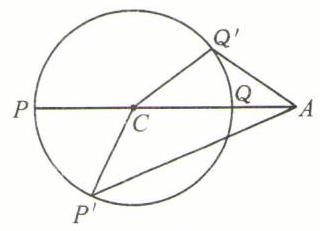
\includegraphics[width=0.2\textwidth]{bodyxb/src/bo_d20cdrf7aajc73bfmvhg_49_1130_826_320_231_0.jpg}
\end{center}


(第 34 题)

35. D 提示: 圆心到直线的距离为 $\dfrac{\left| 0 + 0 - r\right| }{\sqrt{{1}^{2} + {1}^{2}}} = \dfrac{r}{\sqrt{2}}$ ,圆的半径为 $\sqrt{r}$ ,由题意, $\dfrac{r}{\sqrt{2}} = \sqrt{r}$ ,因此 $r = 2$ .

36. (1) $x - y - 3 = 0,x + y - 3 = 0$ 提示: 圆的标准方程为 ${\left( x - 4\right) }^{2} + {\left( y - 1\right) }^{2} = 5$ ,圆心为 $C\left( {4,1}\right)$ . 一个圆里最长的弦是直径,故最长的弦所在直线为直线 ${CP} : y - 0 = \dfrac{1 - 0}{4 - 3}\left( {x - 3}\right)$ ,整理得 $x - y - 3 = 0$ . 最短的弦所在直线是过点 $P$ ,且与直线 ${CP}$ 垂直的直线 (见注释),由于 ${k}_{CP} = 1$ ,因此所求直线为 $y - 0 =  - \left( {x - 3}\right)$ ,整理得 $\vv{x} + y - 3 = 0$ . 注: 过任意圆 $C$ 内一定点 $P$ 作弦 $l$ ,若给定圆的半径为 $R$ 、弦心距为 $d$ ,则弦长为 $L = 2\sqrt{{R}^{2} - {d}^{2}}$ ,欲使 $L$ 最大,则 $d$ 应最小,可取 0, 此时弦过圆心,即为一条直径. 欲使 $L$ 最小,则 $d$ 应最大,利用直角三角形的性质可知 ${d}_{\max } = \left| {CP}\right|$ ,此时 $l\bot {CP}$ .

(2) $x + y - 4 = 0$ 提示:圆的标准方程为: ${\left( x - 2\right) }^{2} + {y}^{2} = 9$ ,圆心为 $C\left( {2,0}\right)$ ,根据垂径定理, ${CP} \bot  {AB}$ , ${k}_{AB} =  - \dfrac{1}{{k}_{CP}} =$ -1,因此直线 ${AB}$ 的方程为: $y - 1 =  - \left( {x - 3}\right)$ ,整理得 $x + y - 4 = 0$ .

(3) $\left( {-\dfrac{3}{10},\dfrac{1}{10}}\right)$ 提示: 设 $A\left( {{x}_{1},{y}_{1}}\right) ,B\left( {{x}_{2},{y}_{2}}\right)$ ,将直线方程代入曲线,整理得 ${10}{x}^{2} + {6x} - 3 = 0$ ,故 $\dfrac{{x}_{1} + {x}_{2}}{2} =  - \dfrac{3}{10}$ , $\dfrac{{y}_{1} + {y}_{2}}{2} = 3 \times  \dfrac{{x}_{1} + {x}_{2}}{2} + 1 = \dfrac{1}{10}$ (或直接代入直线方程),故弦 ${AB}$ 的中点为 $\left( {-\dfrac{3}{10},\dfrac{1}{10}}\right)$ .

37. (1) $\sqrt{14}$ 提示:方法一:圆心到直线的距离为 $\dfrac{\left| 0 - 0 - 1\right| }{\sqrt{{1}^{2} + {1}^{2}}} = \dfrac{\sqrt{2}}{2}$ ,圆半径为 2,因此所求弦长为 $2\sqrt{{2}^{2} - {\left( \dfrac{\sqrt{2}}{2}\right) }^{2}} = \sqrt{14}$ . 方法二: 将直线方程代入圆,消去 $y$ ,整理得 $2{x}^{2} - {2x} - 3 = 0$ ,因此 ${x}_{1} + {x}_{2} = 1,{x}_{1}{x}_{2} =  - \dfrac{3}{2}$ ,所求弦长为 $\sqrt{1 + {1}^{2}} \cdot  {x}_{1}$  $- {x}_{2} \mid   = \sqrt{2} \cdot  \sqrt{{\left( {x}_{1} + {x}_{2}\right) }^{2} - 4{x}_{1}{x}_{2}} = \sqrt{14}.$

(2)2 提示:圆的标准方程为: ${\left( x - a\right) }^{2} + {\left( y + a\right) }^{2} =  - {\left( a - 1\right) }^{2} + 2$ ,当且仅当 $a = 1$ 时,半径最大. 此时,圆与 $y$ 轴 ( $x =$ 0 )交点满足方程 ${\left( y + 1\right) }^{2} = 1$ ,因此 ${y}_{1} = 0,{y}_{2} =  - 2$ ,在 $y$ 轴上截得的弦长为 2 .

(3) ${\left( x - 2\right) }^{2} + {\left( y + 1\right) }^{2} = 4$ 提示: 圆心到直线的距离为 $d = \dfrac{\left| 2 + 1 - 1\right| }{\sqrt{{1}^{2} + {1}^{2}}} = \sqrt{2}$ ,圆的半径 $r$ 满足: ${r}^{2} = {d}^{2} + {\left( \dfrac{2\sqrt{2}}{2}\right) }^{2}$ ,

$\therefore r = 2,\;\therefore \;$ 圆的方程为: ${\left( x - 2\right) }^{2} + {\left( y + 1\right) }^{2} = 4$ .

(4) $\pm  \dfrac{\sqrt{3}}{3}$ 提示: 设直线方程为 $l : y - 2 = {kx}$ ,其中 $k$ 为斜率. 圆心到直线的距离为 $d = \dfrac{\left| 0 - 0 + 2\right| }{\sqrt{{k}^{2} + 1}}$ ,此外 $d$ 还满足 ${d}^{2} +$  ${\left( \dfrac{2}{2}\right) }^{2} = {r}^{2} = {2}^{2},\;\therefore \;$ 直线 $l$ 的斜率为 $k =  \pm  \dfrac{\sqrt{3}}{3}$ .

38. (1) 3 提示: 方法一: 点 $M$ 到圆心 $C$ 的距离为 $\left| {MC}\right|  = \sqrt{10}$ ,圆的半径为 $r = 1$ ,设切点为 $N$ ,则在 $\bigtriangleup {MNC}$ 中, $\angle {MNC} =$  ${90}^{ \circ  }$ ,因此 $\left| {MN}\right|  = \sqrt{{\left| MC\right| }^{2} - {r}^{2}} = 3$ . 方法二: 设切点坐标为 $N\left( {{x}_{0},{y}_{0}}\right)$ ,则切线方程为 ${x}_{0}x + {y}_{0}y = 1$ ,代入点 $M$ 的坐标,且点 $N$ 的坐标满足圆的方程, $\therefore \left\{  \begin{array}{l} {x}_{0} + 3{y}_{0} = 1, \\  {x}_{0}^{2} + {y}_{0}^{2} = 1, \end{array}\right.$ 消去 ${x}_{0}$ ,整理得 ${10}{y}_{0}^{2} - 6{y}_{0} = 0$ . 另外, $\left| {MN}\right|  =$  $\sqrt{{\left( {x}_{0} - 1\right) }^{2} + {\left( {y}_{0} - 3\right) }^{2}} = \sqrt{{10}{y}_{0}^{2} - 6{y}_{0} + 9} = \sqrt{9} = 3$ (或先解出点 $N$ 的坐标,再求 $\left| {MN}\right|$ ).

(2) ${3x} - {4y} + {25} = 0$ 提示:点 $P$ 就在圆上,因此切线方程为 $- {3x} + {4y} = {25}$ ,即 ${3x} - {4y} + {25} = 0$ .

39. C 提示: 圆的标准方程为 ${\left( x + 2\right) }^{2} + {\left( y - 2\right) }^{2} = 2$ ,注意到圆心(-2,2)恰好在直线上,因此直线被圆截得的弦为直径,长度为 $2\sqrt{2}$ .

40. $C$ 提示:圆心到直线的距离 $d = \dfrac{\left| 0 + 0 + c\right| }{\sqrt{{a}^{2} + {b}^{2}}} = \sqrt{\dfrac{{c}^{2}}{{a}^{2} + {b}^{2}}} = \dfrac{\sqrt{3}}{2},\because 0 < d < 1,\therefore$ 直线与圆相交但直线不过圆心.

41. $B$ 提示: 由题意,圆心到直线的距离等于半径,故 $d = \dfrac{\left| -ab\right| }{\sqrt{{a}^{2} + {b}^{2}}} = 1$ ,整理得 $\left( {{a}^{2} - 1}\right) \left( {{b}^{2} - 1}\right)  = 1$ .

42. $C$ 提示:方法一:圆的标准方程为 ${\left( x - 1\right) }^{2} + {y}^{2} = 4$ . 直线过定点 $A\left( {0,1}\right)$ 且斜率为 $a$ . 定点 $A$ 到圆心的距离是 $\sqrt{2}$ ,小于半径, $\therefore$ 定点 $A$ 在圆内, $\therefore$ 直线与圆必有 2 个公共点. 方法二: 将直线方程代入圆,整理得二次方程: $\left( {{a}^{2} + 1}\right) {x}^{2} +$  $\left( {{2a} - 2}\right) x - 2 = 0,\Delta  = {\left( {2a} - 2\right) }^{2} + 8\left( {{a}^{2} + 1}\right)  > 0,\;\therefore$ 直线与圆必有 2 个公共点.

43. A 提示: 圆心到直线的距离为 $d = \dfrac{\left| -{r}^{2}\right| }{\sqrt{{x}_{0}^{2} + {y}_{0}^{2}}},\because$ 点 $P$ 在圆内, $\therefore {x}_{0}^{2} + {y}_{0}^{2} < {r}^{2},\therefore d > r$ ,即直线与圆相离, 没有公共点.

44. B 提示: 对于圆上一点 $P\left( {x,y}\right) ,\dfrac{y - 2}{x - 1}$ 可以看成是点 $P$ 和点 $A\left( {1,2}\right)$ 所在直线 ${PA}$ 的斜率 (如存在),记 $\dfrac{y - 2}{x - 1} = k$ . 如图, 当直线 ${PA}$ 与圆相切且不垂直于 $x$ 轴时 (图中直线 ${l}_{2}$ ), $k$ 取得最小值. 根据圆心到直线 ${l}_{2} : {kx} - y + \left( {2 - k}\right)  = 0$ 的距离等于半径,得 $\dfrac{\left| 2 - k\right| }{\sqrt{{k}^{2} + 1}} = 1$ ,解得 $k = \dfrac{3}{4},\dfrac{y - 2}{x - 1}$ 的取值范围是 $\left\lbrack  {\dfrac{3}{4}, + \infty }\right)$ .

\begin{center}
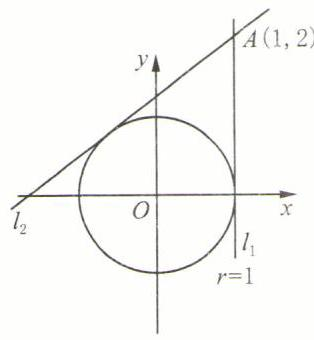
\includegraphics[width=0.2\textwidth]{bodyxb/src/bo_d20cdrf7aajc73bfmvhg_50_266_1296_314_340_0.jpg}
\end{center}


(第 44 题)

\begin{center}
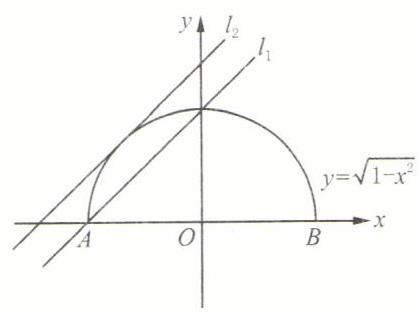
\includegraphics[width=0.3\textwidth]{bodyxb/src/bo_d20cdrf7aajc73bfmvhg_50_646_1319_419_315_0.jpg}
\end{center}


(第 45 题)

\begin{center}
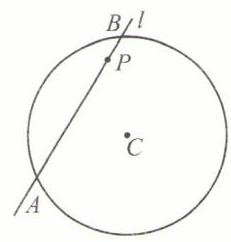
\includegraphics[width=0.2\textwidth]{bodyxb/src/bo_d20cdrf7aajc73bfmvhg_50_1124_1388_231_242_0.jpg}
\end{center}


(第 46 题)

45. $D$ 提示:如图,曲线 $y = \sqrt{1 - {x}^{2}}$ 是圆 ${x}^{2} + {y}^{2} = 1$ 在 $x$ 轴上方的部分 (含 $x$ 轴上的两个端点 $A,B$ ),直线 $l : y = x + m$ 是斜率为 1,在 $y$ 轴上的截距为 $m$ 的直线,当且仅当直线 $l$ 在过半圆的左侧端点 $A$ 的直线 ${l}_{1}$ 和与半圆相切的直线 ${l}_{2}$ 之间 (含直线 ${l}_{1}$ ,不含直线 ${l}_{2}$ )时,直线与半圆有两个不同的公共点. 直线 ${l}_{1}$ 在 $y$ 轴上的截距为 1,直线 ${l}_{2}$ 在 $y$ 轴上的截距为 $\sqrt{2}$ ,故 $m \in  \left\lbrack  {1,\sqrt{2}}\right)$ .

46. D 提示:圆的标准方程为 ${\left( x - 2\right) }^{2} + {y}^{2} = 9$ ,记圆心为 $C\left( {2,0}\right)$ ,易知点 $P\left( {1,2}\right)$ 在圆内. 大、小弓形面积之差最大时,圆心距离直线 $l$ 的距离最大(原因见注释),此时应有 $l \bot  {CP}.{k}_{CP} =  - 2$ ,故 ${k}_{l} = \dfrac{1}{2},l : y - 2 = \dfrac{1}{2}\left( {x - 1}\right)$ ,整理得 $x - {2y} + 3 =$ 0. 注:如图,过圆 $C$ 内任意一点 $P$ 的直线 $l$ ,交圆 $C$ 于 $A$ , $B$ 两点,则 ${S}_{\text{ 大弓形 }} = {S}_{\text{ 大菊形 ACB }} + {S}_{\bigtriangleup {ACB}}$ , ${S}_{\text{ 小导形 }} = {S}_{\text{ 小扇形 ACB }} -$  ${S}_{\bigtriangleup {ACB}}$ ,另外, ${S}_{\text{ 大射形 ACB }} = {S}_{\square C} - {S}_{\text{ 小扇形 ACB }}$ ,故 ${S}_{\text{ 大弓形 }} - {S}_{\text{ 小弓形 }} = {S}_{\square C} - 2 \cdot  {S}_{\text{ 小弓形 }}$ ,因此大、小弓形面积之差最大时,小弓形面积最小. 若弦对应的圆心角为 $\theta$ ,半径是 $r$ ,则小弓形的面积是 $\dfrac{{r}^{2}}{2}\left( {\theta  - \sin \theta }\right)$ . 对于函数 $f\left( \theta \right)  = \theta  - \sin \theta ,\theta  \in  \left\lbrack  {0,\pi }\right\rbrack$ .

$\because {f}^{\prime }\left( \theta \right)  - 1 - \cos \theta  > 0,\therefore y = f\left( \theta \right)$ 在 $\theta  \in  \left\lbrack  {0,\pi }\right\rbrack$ 上单调递增.

47. 如图, $a = 0$ 时, $B = \{ \left( {0,0}\right) \} ,A \cap  B = \varnothing ;a > 0$ 时, ${\left( x - a\right) }^{2} + {y}^{2} = {a}^{2}$ 表示一个圆,除了圆与 $x$ 轴的交点外,均在第一、四象限 $\left( {x > 0}\right)$ ,故只可能与 $y =  - x - 2$ 在第四象限有公共点,为使得 $A \cap  B = \varnothing$ ,则圆心到直线的距离 $d = \dfrac{\left| a + 0 + 2\right| }{\sqrt{{1}^{2} + {1}^{2}}} > a \Rightarrow  a + 2 > \sqrt{2}a$  $\Rightarrow  0 < a < 2\left( {\sqrt{2} + 1}\right) ;a < 0$ 时,类似地,有 $d = \dfrac{\left| a - 2\right| }{\sqrt{{1}^{2} + {1}^{2}}} >  - a \Rightarrow  2 - a >  - \sqrt{2}a \Rightarrow$  $- 2\left( {\sqrt{2} + 1}\right)  < a < 0$ (或根据对称性也可得到这一点). 综上, $- 2\left( {\sqrt{2} + 1}\right)  < a < 2\left( {\sqrt{2} + 1}\right)$ .

\begin{center}
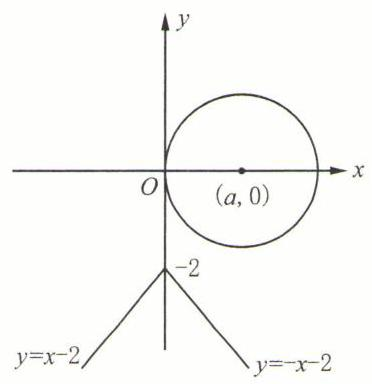
\includegraphics[width=0.3\textwidth]{bodyxb/src/bo_d20cdrf7aajc73bfmvhg_51_1087_130_372_384_0.jpg}
\end{center}


(第 47 题)

48. 当斜率不存在时,直线为 $l : x = 4$ ,与圆相离. 当斜率存在时,设直线方程为 $l : y = k(x$  $- 4)$ ,圆心到直线 $l$ 的距离为: $d = \dfrac{\left| -4k\right| }{\sqrt{{k}^{2} + 1}}$ .

(1)令 $d = r = 2\sqrt{2}$ ,解得 $k =  \pm  1$ ,因此直线 $l$ 的倾斜角 $\theta$ 为 $\dfrac{\pi }{4}$ 或 $\dfrac{3\pi }{4}$ .

(2)令 $d < r = 2\sqrt{2}$ ,解得 $- 1 < k < 1$ ,因此直线 $l$ 的倾斜角 $\theta$ 的取值范围是 $\left\lbrack  {0,\dfrac{\pi }{4}}\right)  \cup  \left( {\dfrac{3\pi }{4},\pi }\right)$ .

(3)令 $d > r = 2\sqrt{2}$ ,解得 $k <  - 1$ 或 $k > 1$ ,另外斜率不存在也满足要求,故直线 $l$ 的倾斜角 $\theta$ 的取值范围是 $\left( {\dfrac{\pi }{4},\dfrac{3\pi }{4}}\right)$ .

49. (1)由题意,设圆心坐标为 $C\left( {{3t},t}\right)$ ,圆心 $C$ 与 $y$ 轴 $\left( {x = 0}\right)$ 相切 $\Leftrightarrow  \left| {3t}\right|  = r$ ( $r$ 是半径)；圆心 $C$ 到直线 $y = x$ 的距离为 $d =$  $\dfrac{\left| 3t - t\right| }{\sqrt{{1}^{2} + {1}^{2}}} = \sqrt{2}\left| t\right|$ ,截得的弦长为 $2\sqrt{{r}^{2} - {d}^{2}} = 2\sqrt{7}\left| t\right|  = 2\sqrt{7}$ ,因此 $t =  \pm  1$ ,圆 $C$ 的方程为 ${\left( x - 3\right) }^{2} + {\left( y - 1\right) }^{2} = 9$ 或 ${\left( x + 3\right) }^{2} + {\left( y + 1\right) }^{2} = 9.$

(2)由于两点之间线段最短,故过两点且面积最小的圆,是以过这两点的线段为直径的圆. 为求圆的方程,我们只需知道圆心和直径即可. 将直线 $y =  - {2x} - 4$ 代入圆的方程,整理得 $5{x}^{2} + {26x} + {27} = 0\left( {\Delta  > 0}\right)$ ,故 ${x}_{1} + {x}_{2} =  - \dfrac{26}{5},{x}_{1}{x}_{2} =$  $\dfrac{27}{5},{y}_{1} + {y}_{2} =  - 2\left( {{x}_{1} + {x}_{2}}\right)  - 8 = \dfrac{12}{5}.\;\therefore$ 圆和直线公共点连接后,所得线段的中点为 $\left( {\dfrac{{x}_{1} + {x}_{2}}{2},\dfrac{{y}_{1} + {y}_{2}}{2}}\right)  =$  $\left( {-\dfrac{13}{5},\dfrac{6}{5}}\right)$ ,距离 (直径) 为 $\sqrt{1 + {2}^{2}}\left| {{x}_{2} - {x}_{1}}\right|  = \sqrt{5}\sqrt{{\left( {x}_{1} + {x}_{2}\right) }^{2} - 4{x}_{1}{x}_{2}} = \sqrt{\dfrac{136}{5}},\therefore$ 所求圆的方程为 ${\left( x + \dfrac{13}{5}\right) }^{2} + {\left( y - \dfrac{6}{5}\right) }^{2} = \dfrac{34}{5}.$

(3)当倾斜角 $\theta  = \dfrac{\pi }{2}$ 时,直线 $l : x = 3$ 与圆交于点 $\left( {3, \pm  \sqrt{7}}\right) ,{S}_{\bigtriangleup {AOB}} = 3\sqrt{7}$ ；当倾斜角 $\theta  \neq  \dfrac{\pi }{2}$ 时,设直线 $l : y = k\left( {x - 3}\right)$ ,圆心到直线 $l$ 的距离为 $d = \dfrac{\left| -3k\right| }{\sqrt{{k}^{2} + 1}},{S}_{\bigtriangleup {AOB}} = \dfrac{1}{2} \cdot  2\sqrt{{r}^{2} - {d}^{2}} \cdot  d = \sqrt{-{\left( {d}^{2} - \dfrac{1}{2}{r}^{2}\right) }^{2} + \dfrac{1}{4}{r}^{4}}$ ,当 ${d}^{2} - \dfrac{1}{2}{r}^{2} = 0$ 即 $k$

$=  \pm  2\sqrt{2}$ 时, ${S}_{\bigtriangleup {AOB}}$ 有最大值,为 8 (大于 $3\sqrt{7}$ ). 因此,当 $\theta  = \arctan 2\sqrt{2}$ 或 $\theta  = \pi  - \arctan 2\sqrt{2}$ 时, $\bigtriangleup  {AOB}$ 面积最大,最大值为 8. 注意:我们这里没有将 ${S}_{\bigtriangleup {AOB}}$ 最后写成关于 $k$ 的函数,这样做可以大大简化计算,但此时一定要保证能取到相应的值.

50. (1) 由题意,设所求切线方程为 ${2x} + {3y} + m = 0$ . 圆的标准方程为 ${\left( x - 1\right) }^{2} + {y}^{2} = 4$ ,圆心到直线的距离等于半径,故 $d =$  $\dfrac{\left| 2 \cdot  1 + 0 + m\right| }{\sqrt{{2}^{2} + {3}^{2}}} = 2,\;\therefore \;m =  - 2 \pm  2\sqrt{13}$ ,所求切线方程为 ${2x} + {3y} - 2 \pm  2\sqrt{13} = 0$ .

(2)圆的标准方程为 ${\left( x - 1\right) }^{2} + {y}^{2} = 4$ . 若过点(3,1)的直线 $l$ 的斜率不存在,则 $l : x = 3$ ,与圆只有一个公共点(3,0)；若过点(3,1)的直线 $l$ 斜率存在,设 $l : y - 1 = k\left( {x - 3}\right)$ ,圆心到直线 $l$ 的距离为 $d = \dfrac{\left| k - 3k + 1\right| }{\sqrt{{k}^{2} + 1}} = r = 2$ ,

$\therefore k =  - \dfrac{3}{4}$ . 综上,所求切线方程为 $x = 3$ 或 ${3x} + {4y} - {13} = 0$ .

(3)圆的标准方程为 ${\left( x - 2\right) }^{2} + {\left( y - 2\right) }^{2} = 1$ ,反射光线一定过点 $P\left( {-3,3}\right)$ 关于 $x$ 轴的对称点 ${P}^{\prime }\left( {-3, - 3}\right)$ ,且斜率存在 (否则与圆无公共点). 因此,设反射光线所在直线方程为 ${l}^{\prime } : y + 3 = {k}^{\prime }\left( {x + 3}\right)$ ,圆心到直线 ${l}^{\prime }$ 的距离为 $d =$  $\dfrac{\left| 2{k}^{\prime } - 2 + 3{k}^{\prime } - 3\right| }{\sqrt{{k}^{\prime 2} + 1}} = r = 1$ ,解得 ${k}^{\prime } = \dfrac{4}{3}$ 或 ${k}^{\prime } = \dfrac{3}{4}$ . 入射光线的斜率 $k$ 和反射光线的斜率 ${k}^{\prime }$ 满足 $k =  - {k}^{\prime },\therefore \lambda$ 射光线 $l$ 所在直线的方程为 $y - 3 =  - \dfrac{4}{3}\left( {x + 3}\right)$ 或 $y - 3 =  - \dfrac{3}{4}\left( {x + 3}\right)$ ,整理得 ${4x} + {3y} + 3 = 0$ 或 ${3x} + {4y} - 3 = 0$ .

51. (1) 由题意,设圆心 $C\left( {t, - {4t}}\right)$ . 方法一: 由圆心到直线 $x + y - 1 = 0$ 的距离等于半径 $\left| {CP}\right|$ ,得 $d = \dfrac{\left| t - 4t - 1\right| }{\sqrt{{1}^{2} + {1}^{2}}} =$  $\sqrt{{\left( t - 3\right) }^{2} + {\left( -4t + 2\right) }^{2}}$ ,解得 $t = 1$ . . . 圆心 $C\left( {1, - 4}\right)$ ,半径 $\left| {CP}\right|  = 2\sqrt{2}$ ,圆 $C$ 的方程为 ${\left( x - 1\right) }^{2} + {\left( y + 4\right) }^{2} = 8$ . 方法二: 由 ${l}_{CP}$ 与直线 $x + y - 1 = 0$ 垂直,可得 ${k}_{CP} \cdot  \left( {-1}\right)  =  - 1$ ,即 $\dfrac{-{4t} + 2}{t - 3} = 1$ ,解得 $t = 1$ ,下同方法一.

(2)关键是确定圆心. 圆心在过点 $Q\left( {4, - 1}\right)$ 且垂直于直线 $x - {6y} - {10} = 0$ 的直线 ${l}_{1}$ 上,也在线段 ${QM}$ 的垂直平分线 ${l}_{2}$ 上. ${k}_{{l}_{1}} =  - 6,\therefore {l}_{1} : y + 1 =  - 6\left( {x - 4}\right) ;{k}_{QM} = \dfrac{7}{5}$ ,线段 ${QM}$ 的中点为 $\left( {\dfrac{13}{2},\dfrac{5}{2}}\right) ,\therefore {l}_{2} : y - \dfrac{5}{2} =$  $- \dfrac{5}{7}\left( {x - \dfrac{13}{2}}\right) .{l}_{1}$ 与 ${l}_{2}$ 交于点(3,5),半径 $r = \sqrt{37},\therefore$ 圆 $C$ 的方程为 ${\left( x - 3\right) }^{2} + {\left( y - 5\right) }^{2} = {37}$ .

(3) 由题意,设圆心 $C\left( {t, - {2t}}\right)$ ,由圆心到直线 $x - y - 1 = 0$ 的距离等于半径,得 $d = \dfrac{\left| t + {2t} - 1\right| }{\sqrt{{1}^{2} + {1}^{2}}} =$  $\sqrt{{\left( t - 2\right) }^{2} + {\left( -2t + 1\right) }^{2}}$ ,解得 $t = 1$ 或 $t = 9$ ,对应圆心 $C\left( {1, - 2}\right)$ 及半径 $\sqrt{2}$ 或圆心 $C\left( {9, - {18}}\right)$ 及半径 ${13}\sqrt{2}$ ,

$\therefore$ 圆 $C$ 的方程为 ${\left( x - 1\right) }^{2} + {\left( y + 2\right) }^{2} = 2$ 或 ${\left( x - 9\right) }^{2} + {\left( y + {18}\right) }^{2} = {338}$ .

52. (1) 记圆心为 $C$ . 当 ${x}_{0} = a \pm  R$ 时, ${y}_{0} = b$ ,切线方程显然为 $x = a \pm  R$ ,满足 $\left( {{x}_{0} - a}\right) \left( {x - a}\right)  + \left( {{y}_{0} - b}\right) \left( {y - b}\right)  = {R}^{2}$ 的形式,以下提供三种方法,证明 ${x}_{0} \neq  a \pm  R$ 时 $\left( {{y}_{0} \neq  b}\right)$ ,切线方程同样满足这一形式.

方法一: 若 ${x}_{0} = a$ ,则 ${y}_{0} = b \pm  R$ ,切线方程显然为 $y = b \pm  R$ ,仍然满足 $\left( {{x}_{0} - a}\right) \left( {x - a}\right)  + \left( {{y}_{0} - b}\right) \left( {y - b}\right)  = {R}^{2}$ 的形式. 若 ${x}_{0} \neq  a$ ,则 ${k}_{CP} = \dfrac{{y}_{0} - b}{{x}_{0} - a} \neq  0$ ,切线垂直于直线 ${CP}$ ,因此切线斜率为 $- \dfrac{{x}_{0} - a}{{y}_{0} - b}$ ,切线方程为 $y - {y}_{0} =  - \dfrac{{x}_{0} - a}{{y}_{0} - b}(x$  $\left. {-{x}_{0}}\right)$ ,即 $\left( {{x}_{0} - a}\right) \left( {x - {x}_{0}}\right)  + \left( {{y}_{0} - b}\right) \left( {y - {y}_{0}}\right)  = 0$ ,稍作变形: $\left( {{x}_{0} - a}\right) \left( {x - a + a - {x}_{0}}\right)  + \left( {{y}_{0} - b}\right)  \cdot  \left( {y - b + b - {y}_{0}}\right)$  $= \left( {{x}_{0} - a}\right) \left( {x - a}\right)  + \left( {{y}_{0} - b}\right) \left( {y - b}\right)  - {\left( {x}_{0} - a\right) }^{2} - {\left( {y}_{0} - b\right) }^{2} = \left( {{x}_{0} - a}\right) \left( {x - a}\right)  + \left( {{y}_{0} - b}\right) \left( {y - b}\right)  - {R}^{2} = 0,$

$\therefore$ 切线方程为 $\left( {{x}_{0} - a}\right) \left( {x - a}\right)  + \left( {{y}_{0} - b}\right) \left( {y - b}\right)  = {R}^{2}$ .

方法二: 由于斜率存在,故设切线方程为 $y - {y}_{0} = k\left( {x - {x}_{0}}\right)$ ,由圆心到切线的距离等于半径,得 $d =$  $\dfrac{\left| ka - b + {y}_{0} - k{x}_{0}\right| }{\sqrt{{k}^{2} + 1}} = R$ ,注意到 ${\left( {x}_{0} - a\right) }^{2} + {\left( {y}_{0} - b\right) }^{2} = {R}^{2}$ ,故整理方程得 ${\left\lbrack  \left( {y}_{0} - b\right) k + \left( {x}_{0} - a\right) \right\rbrack  }^{2} = 0$ ,

故 $k =  - \dfrac{{x}_{0} - a}{{y}_{0} - b}$ ,切线方程为 $y - {y}_{0} =  - \dfrac{{x}_{0} - a}{{y}_{0} - b}\left( {x - {x}_{0}}\right)$ ,用方法一的技巧,整理得切线方程为 $\left( {{x}_{0} - a}\right) \left( {x - a}\right)  + \left( {y}_{0}\right.$  $- b)\left( {y - b}\right)  = {R}^{2}$ .

方法三:由于斜率存在,故设切线方程为 $y - {y}_{0} = k\left( {x - {x}_{0}}\right)$ ,代入圆的方程 ${\left( x - a\right) }^{2} + {\left( y - b\right) }^{2} = {R}^{2}$ ,

整理得 $\left( {1 + {k}^{2}}\right) {x}^{2} + \left( {{2kt} - {2a}}\right) x + {t}^{2} + {a}^{2} - {R}^{2} = 0$ (其中 $t =  - k{x}_{0} + {y}_{0} - b$ ). 令 $\Delta  = 4{\left( kt - a\right) }^{2} - 4\left( {1 + {k}^{2}}\right) \left( {{t}^{2} + {a}^{2} - }\right.$  $\left. {R}^{2}\right)  = 0$ ,整理得 ${\left( t + ka\right) }^{2} = \left( {1 + {k}^{2}}\right) {R}^{2}$ . 再代入 $t =  - k{x}_{0} + {y}_{0} - b$ 并注意到 ${\left( {x}_{0} - a\right) }^{2} + {\left( {y}_{0} - b\right) }^{2} = {R}^{2}$ ,进一步整理得 ${\left\lbrack  \left( {y}_{0} - b\right) k + \left( {x}_{0} - a\right) \right\rbrack  }^{2} = 0$ ,故 $k =  - \dfrac{{x}_{0} - a}{{y}_{0} - b}$ ,切线方程为 $y - {y}_{0} =  - \dfrac{{x}_{0} - a}{{y}_{0} - b}\left( {x - {x}_{0}}\right)$ ,用方法一的技巧,整理得切线方程为 $\left( {{x}_{0} - a}\right) \left( {x - a}\right)  + \left( {{y}_{0} - b}\right) \left( {y - b}\right)  = {R}^{2}$ .

(2)不难验证,点 $A$ 就在圆上,运用前一小问的结论,切线方程为 $\left( {1 - 3}\right) \left( {x - 3}\right)  + \left( {2 + 1}\right) \left( {y + 1}\right)  = {13}$ ,整理得 ${2x} - {3y} + 4$  $= 0$ .

53. (1) 设 $A,B$ 两点的坐标分别是 $A\left( {{x}_{A},{y}_{A}}\right) ,B\left( {{x}_{B},{y}_{B}}\right)$ ,根据圆的切线公式,有 ${l}_{PA} : {x}_{A}x + {y}_{A}y = {r}^{2},{l}_{PB} : {x}_{B}x + {y}_{B}y =$  ${r}^{2}$ . 代入点 $P\left( {{x}_{0},{y}_{0}}\right)$ ,有 $\left\{  \begin{array}{l} {x}_{A}{x}_{0} + {y}_{A}{y}_{0} = {r}^{2}, \\  {x}_{B}{x}_{0} + {y}_{B}{y}_{0} = {r}^{2}, \end{array}\right.$ 可见 $A,B$ 两点都满足方程 ${x}_{0}x + {y}_{0}y = {r}^{2}$ ,由于过 $A,B$ 两点的直线是唯一的,因此弦 ${AB}$ 所在直线方程就是 ${x}_{0}x + {y}_{0}y = {r}^{2}$ .

(2)运用前一小问的结论,因此弦 ${AB}$ 所在直线方程是 ${3x} - {4y} = 4$ ,即 ${3x} - {4y} - 4 = 0$ .

54. (1) 方法一:记圆的圆心为 $C$ . 点 $C$ 到直线 $l : {4x} + {3y} = 2$ 的距离为 $\dfrac{2}{5}$ ,小于圆 $C$ 的半径 2,因此直线与圆 $C$ 相交. 圆上到直线 $l$ 距离最大的点 $P$ ,一定满足 ${PC} \bot  l$ (原因见注释). 因此, ${k}_{PC} = \dfrac{3}{4}$ ,设 ${l}_{PC} : {3x} - {4y} + m = 0$ ,代入 $C\left( {0,0}\right)$ ,得 $m$  $= 0,\therefore {l}_{PC} : {3x} - {4y} = 0$ ,代入圆 $C$ 的方程,解得 ${P}_{1}\left( {-\dfrac{8}{5}, - \dfrac{6}{5}}\right) ,{P}_{2}\left( {\dfrac{8}{5},\dfrac{6}{5}}\right)$ ,点 ${P}_{1}$ 到直线 $l$ 的距离为 $\dfrac{12}{5}$ ; 点

${P}_{2}$ 到直线 $l$ 的距离为 $\dfrac{8}{5}$ ,舍去. 综上,点 $P$ 的坐标为 $P\left( {-\dfrac{8}{5}, - \dfrac{6}{5}}\right)$ . 注: 如图,圆 $C$ 和直线 $l$ 相交,直线 $m$ 是过圆心

$C$ 且平行于直线 $l$ 的直线,和圆交于 $A,B$ 两点,直线 $m$ 与直线 $l$ 的距离为 $d.P$ 是圆 $C$ 上任意一点,射线 ${CA}$ 逆时针旋转 $\theta$ 角到射线 ${CP}$ ,则点 $P$ 到直线 $l$ 的距离为 $\left| {d - r\sin \theta }\right|$ ,其最大值为 $d + r$ ,此时 $\theta  = \dfrac{3}{2}\pi$ (若 $d = 0$ ,则 $\theta  = \dfrac{1}{2}\pi$ 或 $\theta  = \dfrac{3}{2}\pi$ ),也即圆上到直线 $l$ 距离最大的点 $P$ ,一定满足 ${PC}\bot l$ . 读者可以用类似方法进一步讨论直线 $l$ 与圆 $C$ 相切或相离时,圆上到直线 $l$ 距离最大的点 $P$ 是否仍然有相同的特点.

方法二: (参数方程) 设点 $P\left( {2\cos \theta ,2\sin \theta }\right) \left( {0 \leq  \theta  < {2\pi }}\right)$ ,则点 $P$ 到直线 $l : {4x} + {3y} = 2$ 的距离为 $d =$  $\dfrac{\left| 8\cos \theta  + 6\sin \theta  - 2\right| }{5} = \dfrac{\left| {10}\sin \left( \theta  + \varphi \right)  - 2\right| }{5}\left( {\tan \varphi  = \dfrac{4}{3}}\right)$ ,当且仅当 $\sin \left( {\theta  + \varphi }\right)  =  - 1$ ,即 $\theta  = \dfrac{3}{2}\pi  - \arctan \dfrac{4}{3}$ 时,有 ${d}_{\max }$  $= \dfrac{12}{5}$ ,此时点 $P$ 的坐标为 $\left( {-\dfrac{8}{5}, - \dfrac{6}{5}}\right)$ .

\begin{center}
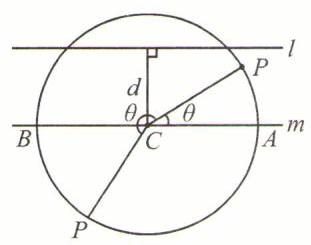
\includegraphics[width=0.2\textwidth]{bodyxb/src/bo_d20cdrf7aajc73bfmvhg_53_448_345_311_245_0.jpg}
\end{center}


[第 54(1)题]

\begin{center}
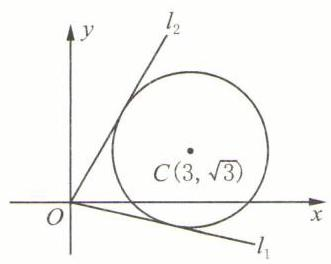
\includegraphics[width=0.2\textwidth]{bodyxb/src/bo_d20cdrf7aajc73bfmvhg_53_818_323_331_264_0.jpg}
\end{center}


[第 54(2)题]

(2)如图, $\dfrac{y}{x}$ 可以看成是 $\dfrac{y - 0}{x - 0}$ ,即过圆上的点 $P$ 与原点 $O$ 所在直线的斜率 ${k}_{PO}$ ,斜率的变化范围可以由点 $O$ 向圆引出的两条切线 ${l}_{1},{l}_{2}$ 来确定. 设直线 ${l}_{OP} : y = {kx}$ ,令圆心到直线的距离等于半径,可得 $d = \dfrac{\left| 3k - \sqrt{3}\right| }{\sqrt{{k}^{2} + 1}} = r = \sqrt{6}$ ,解得 ${k}_{1} =$  $- 2 + \sqrt{3},{k}_{2} = 2 + \sqrt{3},\;\therefore \; - 2 + \sqrt{3} \leq  \dfrac{y}{x} \leq  2 + \sqrt{3},\dfrac{y}{x}$ 的最大值为 $2 + \sqrt{3}$ .

55. 如图,曲线 $C$ 是圆 ${x}^{2} + {y}^{2} = 3$ 在 $y$ 轴右侧的部分 (含 $y$ 轴上的两个端点 $A\left( {0, - \sqrt{3}}\right)$ , $B\left( {0,\sqrt{3}}\right)$ ). 直线 $l$ 过定点 $P\left( {-1, - 3}\right)$ ,斜率为 $m$ . 定点 $P$ 在第三象限,且在端点 $A$ 下方. 在 $m$ 变化过程中,有三个关键位置: ${l}_{1}$ : 过点 $P$ 且与圆 ${x}^{2} + {y}^{2} = 3$ 在第四象限相切的直线,由圆心到直线的距离等于半径,得 $d = \dfrac{\left| m - 3\right| }{\sqrt{{m}^{2} + 1}} = \sqrt{3},m > 0$ ,解得 ${m}_{1} = \dfrac{-3 + \sqrt{21}}{2};{l}_{2}$ : 直线 ${PA}$ , 其斜率 ${m}_{2} =  - \sqrt{3} + 3;{l}_{3}$ : 直线 ${PB}$ ,其斜率 ${m}_{3} = \sqrt{3} + 3$ .

\begin{center}
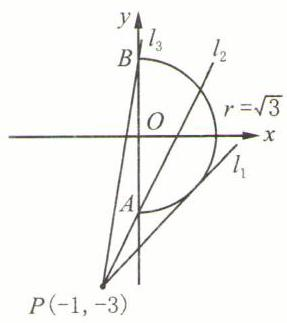
\includegraphics[width=0.2\textwidth]{bodyxb/src/bo_d20cdrf7aajc73bfmvhg_53_1166_868_287_323_0.jpg}
\end{center}


(第 55 题)

(1)当直线在从 ${l}_{2}$ 逆时针旋转到 ${l}_{3}$ 的过程中 (不含 ${l}_{2}$ ,含 ${l}_{3}$ ) 或为 ${l}_{1}$ 时, 即 $- \sqrt{3} + 3 < m \leq  \sqrt{3} + 3$ 或 $m = \dfrac{-3 + \sqrt{21}}{2}$ 时,直线 $l$ 与曲线 $C$ 只有一个公共点.

(2)当直线在从 ${l}_{1}$ 逆时针旋转到 ${l}_{2}$ 的过程中 $\left( {\text{ 不含 }{l}_{1},\text{ 含 }{l}_{2}}\right)$ ,即 $\dfrac{-3 + \sqrt{21}}{2} < m \leq   - \sqrt{3} + 3$ 时,直线 $l$ 与曲线 $C$ 有两个不同公共点.

56. (1) 实数 $x$ , $y$ 满足的方程是一个圆的方程,其标准方程为 ${\left( x - 1\right) }^{2} + {\left( y + 2\right) }^{2} = {25}$ ,记圆心坐标为 $C\left( {1, - 2}\right)$ . 方法一: $L$  $= {x}^{2} + {y}^{2}$ 可以视作是圆上任意一点 $P\left( {x,y}\right)$ 到原点的距离的平方,而原点 $O$ 在圆 $C$ 内部. 我们在本章第 34 题的注释中讨论过,圆 $C$ 上到该圆内一点 $O$ 的距离最短的点为线段 ${CO}$ 延长线与圆 $C$ 的公共点,因此 ${l}_{CO} : y =  - {2x}$ ,代入圆 $C$ 的方程,且注意到 $x < 0$ ,故 $x = 1 - \sqrt{5},{L}_{\min } = {x}^{2} + {y}^{2} = 5{x}^{2} = {30} - {10}\sqrt{5}$ ,此时 $P\left( {1 - \sqrt{5},2\sqrt{5} - 2}\right)$ . 方法二: (参数方程)将 $P\left( {x,y}\right)$ 写成 $P\left( {1 + 5\cos \theta , - 2 + 5\sin \theta }\right) \left( {0 \leq  \theta  < {2\pi }}\right)$ ,则 $L = {x}^{2} + {y}^{2} = {2x} - {4y} + {20} = {30} - {10}\left( {2\sin \theta  - \cos \theta }\right)  = {30}$  $- {10}\sqrt{5}\sin \left( {\theta  - \varphi }\right) \left( {\tan \varphi  = \dfrac{1}{2}}\right)$ . 当且仅当 $\sin \left( {\theta  - \varphi }\right)  = 1$ ,即 $\theta  = \dfrac{\pi }{2} + \arctan \dfrac{1}{2}$ 时, ${L}_{\min } = {30} - {10}\sqrt{5}$ ,此时点 $P$ 的坐标为 $\left( {1 - \sqrt{5},2\sqrt{5} - 2}\right)$ .

(2)实数 $x$ , $y$ 满足的方程是一个圆的方程,其标准方程为 ${\left( x - 1\right) }^{2} + {\left( y + 2\right) }^{2} = 5$ ,记圆心坐标为 $C\left( {1, - 2}\right)$ . 方法一: 记 $L = x - {2y}$ ,则 $l : y = \dfrac{x}{2} - \dfrac{L}{2}$ ,是斜率为 $\dfrac{1}{2}$ ,在 $y$ 轴上的截距为 $- \dfrac{L}{2}$ 的直线,现欲求 $L$ 的最大值,则 $- \dfrac{L}{2}$ 应最小. 如图,当 $l$ 与圆 $C$ 相切且切点在第四象限时, $- \dfrac{L}{2}$ 最小. 此时,圆心到直线的距离等于半径,故 $d =$  $\dfrac{\left| 1 + 2 \cdot  2 - L\right| }{\sqrt{{1}^{2} + {2}^{2}}} = r = \sqrt{5},L > 0$ ,解得 ${L}_{\max } = {10}$ ,此时点 $P$ 的坐标为 $P\left( {2, - 4}\right)$ . 方法二: 记 $L = x - {2y} = \dfrac{1}{2}\left( {{x}^{2} + {y}^{2}}\right)$ ,欲求 $L$ 的最大值,即求 ${x}^{2} + {y}^{2}$ 的最大值, ${x}^{2} + {y}^{2}$ 是点 $P\left( {x,y}\right)$ 到原点的距离的平方,原点恰好在圆 $C$ 上. 我们在本章第 34 题的注释中讨论过,圆 $C$ 上到该圆上一点 $O$ 的距离最长的点为线段 ${OC}$ 延长线与圆 $C$ 的公共点 (直径),因此将 ${l}_{CO},y =  - {2x}$ ,代入圆 $C$ 的方程,且注意到 $x >$

\begin{center}
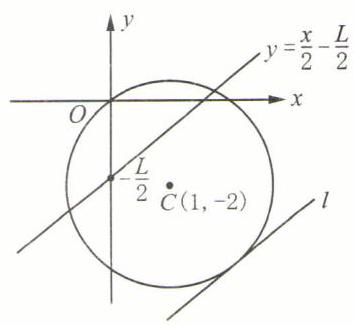
\includegraphics[width=0.3\textwidth]{bodyxb/src/bo_d20cdrf7aajc73bfmvhg_53_1102_1686_354_326_0.jpg}
\end{center}


(第 56 题)

0,故 $x = 2,{L}_{\max } = \dfrac{1}{2}\left( {{x}^{2} + {y}^{2}}\right)  = \dfrac{5}{2}{x}^{2} = {10}$ ,此时点 $P$ 坐标为 $P\left( {2, - 4}\right)$ . 方法三: 将 $P\left( {x,y}\right)$ 写成 $P\left( {1 + \sqrt{5}\cos \theta , - 2 + \sqrt{5}\sin \theta }\right) \left( {0 \leq  \theta  < {2\pi }}\right)$ ,则 $L = x - {2y} = 5 - \sqrt{5}\left( {2\sin \theta  - \cos \theta }\right)  = 5 - 5\sin \left( {\theta  - \varphi }\right) \left( {\tan \varphi  = \dfrac{1}{2}}\right)$ . 当且仅当 $\sin \left( {\theta  - \varphi }\right)  =  - 1$ ,即 $\theta  = \dfrac{3\pi }{2} + \arctan \dfrac{1}{2}$ 时, ${L}_{\max } = {10}$ ,此时点 $P$ 坐标为 $P\left( {2, - 4}\right)$ .

(3) 设动点 $P\left( {x,y}\right)$ ,则 $L = {\left| PA\right| }^{2} + {\left| PB\right| }^{2} = {\left( x + 1\right) }^{2} + {y}^{2} + {\left( x - 1\right) }^{2} + {y}^{2} = 2\left( {{x}^{2} + {y}^{2}}\right)  + 2$ , $L$ 最小时, ${x}^{2} + {y}^{2}$ 应最小. 另记圆的圆心为 $C\left( {3,4}\right)$ . 方法一: ${x}^{2} + {y}^{2}$ 是点 $P\left( {x,y}\right)$ 到原点 $O$ 的距离的平方,而原点在圆 $C$ 外. 我们在本章第 34 题的注释中讨论过,圆 $C$ 上到该圆外一点 $O$ 的距离最短的点为线段 ${OC}$ 与圆 $C$ 的公共点,因此将 ${l}_{CO} : y = \dfrac{4}{3}x$ ,代入圆 $C$ 的方程,又 $0 \leq  x \leq  3$ (在线段 ${OC}$ 上),故 $\left( {x,y}\right)  = \left( {\dfrac{9}{5},\dfrac{12}{5}}\right)$ ,此时 ${L}_{\min } = {20}$ . 方法二: (参数方程) 将 $P\left( {x,y}\right)$ 写成 $P\left( {3 + 2\cos \theta ,4 + 2\sin \theta }\right) \left( {0 \leq  \theta  < {2\pi }}\right)$ ,则 $L = 2\left( {{x}^{2} + {y}^{2}}\right)  + 2 = {60} + {32}\sin \theta  + {24}\cos \theta  = {60} + {40}\sin \left( {\theta  + \varphi }\right) \left( {\tan \varphi  = \dfrac{3}{4}}\right)$ . 当且仅当 $\sin \left( {\theta  + \varphi }\right)  =  - 1$ ,即 $\theta  = \dfrac{3\pi }{2} - \arctan \dfrac{3}{4}$ 时, ${L}_{\min } = {20}$ ,此时点 $P$ 的坐标为 $P\left( {\dfrac{9}{5},\dfrac{12}{5}}\right)$ .

57. $C$ 提示:转化为标准方程 ${\left( x + 2\right) }^{2} + {\left( y - 2\right) }^{2} = 1$ ,圆心 ${C}_{1}\left( {-2,2}\right)$ ,半径 ${r}_{1} = 1;{\left( x - 2\right) }^{2} + {\left( y - 5\right) }^{2} = {16}$ ,圆心 ${C}_{2}\left( {2,5}\right)$ , 半径 ${r}_{2} = 4$ . $\left| {{C}_{1}{C}_{2}}\right|  = 5 = {r}_{1} + {r}_{2}$ ,因此两圆外切,公切线有 3 条.

58. $B$ 提示:转化为标准方程 ${\left( x - 4\right) }^{2} + {\left( y + 3\right) }^{2} = {36}$ ,圆心 ${C}_{1}\left( {4, - 3}\right)$ ,半径 ${r}_{1} = 6;{x}^{2} + {y}^{2} = {100}$ ,圆心 ${C}_{2}\left( {0,0}\right)$ ,半径 ${r}_{2}$  $= {10}.\left| {{r}_{1} - {r}_{2}}\right|  < \left| {{C}_{1}{C}_{2}}\right|  = 5 < {r}_{1} + {r}_{2}$ ,因此两圆相交.

59. B 提示: 由于两圆的半径都是 1,因此两圆相切只能是外切,故圆心距 $\sqrt{{\left( 0 - 1\right) }^{2} + {\left( b - 2\right) }^{2}} = {r}_{1} + {r}_{2} = 2$ ,解得 $b$  $= 2 \pm  \sqrt{3}$ .

60. (1) ${a}^{2} + {b}^{2} = 4$ 提示:由题意,两圆圆心距等于两圆半径之和,即 $\sqrt{{a}^{2} + {b}^{2}} = 1 + 1$ ,整理得 ${a}^{2} + {b}^{2} = 4$ .

(2) ${\left( x - 1\right) }^{2} + {\left( y + 2\right) }^{2} = {20}$ 或 ${\left( x - 1\right) }^{2} + {\left( y + 2\right) }^{2} = {80}$ 提示:记圆 $B : {x}^{2} + {y}^{2} = {45}$ ,圆心为 $B\left( {0,0}\right) ,{r}_{B} = 3\sqrt{5}$ . 点 $A(1$ , -2) 在圆 $B$ 内部,因此圆 $A,B$ 相切只能是内切, $\therefore \left| {AB}\right|  = \sqrt{5} = \left| {{r}_{B} - {r}_{A}}\right| ,\therefore {r}_{A} = 2\sqrt{5}$ 或 ${r}_{A} = 4\sqrt{5}$ ,

$\therefore$ 圆 $A$ 的方程为 ${\left( x - 1\right) }^{2} + {\left( y + 2\right) }^{2} = {20}$ 或 ${\left( x - 1\right) }^{2} + {\left( y + 2\right) }^{2} = {80}$ .

(3) 外离 提示: 两圆半径均为 $\dfrac{1}{4}$ ,两圆圆心距为 $d = \sqrt{{\left( \sin \alpha  + \dfrac{1}{2}\right) }^{2} + {\left( 1 - 0\right) }^{2}},\alpha  \in  \left( {0,\dfrac{\pi }{2}}\right)$ 时, $d \in  \left( {\dfrac{\sqrt{5}}{2},\dfrac{\sqrt{13}}{2}}\right)$ ,可见 $d$ 总是大于两圆的半径之和 $\dfrac{1}{2}$ ,因此两圆外离.

(4) 0 或 $\pm  \sqrt{6}$ 提示:两圆圆心分别为 ${O}_{1}\left( {0,0}\right) ,{O}_{2}\left( {{2a},1}\right)$ ,半径分别为 ${r}_{1} = 3,{r}_{2} = 2,\left| {{O}_{1}{O}_{2}}\right|  = \sqrt{4{a}^{2} + 1}$ . 若两圆外切, 则 $\left| {{O}_{1}{O}_{2}}\right|  = {r}_{1} + {r}_{2} = 5$ ,解得 $a =  \pm  \sqrt{6}$ ；若两圆内切,则 $\left| {{O}_{1}{O}_{2}}\right|  = \left| {{r}_{1} - {r}_{2}}\right|  = 1$ ,解得 $a = 0$ . 综上,实数 $a = 0$ 或 $\pm  \sqrt{6}$ .

61. $B$ 提示:方法一:圆 ${O}_{1} : {\left( x + a\right) }^{2} + {\left( y + a\right) }^{2} = 1$ ,圆 ${O}_{2} : {\left( x + b\right) }^{2} + {\left( y + b\right) }^{2} = 2$ , ${O}_{1}\left( {-a, - a}\right) ,{r}_{1} = 1,{O}_{2}\left( {-b, - b}\right) ,{r}_{2} = \sqrt{2}$ . 设两圆交于 $A,B$ 两点,当线段恰好为圆 ${O}_{1}$ 的直径时,公共弦长达到最大值,即得两圆公共弦长的最大值为圆 ${O}_{1}$ 的直径 2.

\begin{center}
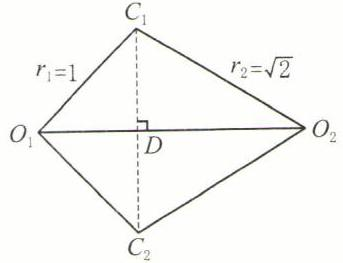
\includegraphics[width=0.2\textwidth]{bodyxb/src/bo_d20cdrf7aajc73bfmvhg_54_1155_1389_343_263_0.jpg}
\end{center}


(第 61 题)

方法二: 如图,两圆圆心分别为 ${O}_{1}\left( {-a, - a}\right) ,{O}_{2}\left( {-b, - b}\right)$ ,半径分别为 ${r}_{1} = 1,{r}_{2} =$  $\sqrt{2}$ ,可见两圆的圆心始终在直线 $y = x$ 上. 两圆的公共弦为 ${C}_{1}{C}_{2},{C}_{1}{C}_{2} \bot  {O}_{1}{O}_{2}$ 于点 $D$ . 设点 $D$ 的坐标为 $D\left( {-t, - t}\right) ,\left| {{C}_{1}D}\right|  = \left| {{C}_{2}D}\right|  = h$ ,则在 $\operatorname{Rt}\bigtriangleup D{C}_{1}{O}_{1}$ 和 $\mathrm{{Rt}}\bigtriangleup D{C}_{1}{O}_{2}$ 中应用勾股定理,可得方程组:

$\left\{  \begin{array}{l} 2{\left( t - a\right) }^{2} + {h}^{2} = 1, \\  2{\left( t - b\right) }^{2} + {h}^{2} = 2, \end{array}\right.$ 解得 $\left\{  \begin{array}{l} t = \dfrac{a + b}{2} + \dfrac{1}{4\left( {a - b}\right) }, \\  h = \sqrt{2 - 2{\left\lbrack  \dfrac{a - b}{2} + \dfrac{1}{4\left( {a - b}\right) }\right\rbrack  }^{2}}. \end{array}\right.$

记 $u = \left| {a - b}\right|$ ,则 $\left| {{O}_{1}{O}_{2}}\right|  = \sqrt{2}u$ ,由两圆相交可知: ${r}_{2} - {r}_{1} < \left| {{O}_{1}{O}_{2}}\right|  = \sqrt{2}u < {r}_{2} + {r}_{1}$ ,故 $1 - \dfrac{\sqrt{2}}{2} < u < 1 + \dfrac{\sqrt{2}}{2}$ ; 此外, $h\left( u\right)  =$  $\sqrt{2 - 2\left( {\dfrac{{u}^{2}}{4} + \dfrac{1}{{16}{u}^{2}} + \dfrac{1}{4}}\right) },h\left( u\right)  \leq  1$ ,当且仅当 $\dfrac{{u}^{2}}{4} = \dfrac{1}{{16}{u}^{2}}$ ,即 $u = \dfrac{\sqrt{2}}{2}$ 时等号成立. 因此,当 $\left| {a - b}\right|  = \dfrac{\sqrt{2}}{2}$ 时,公共弦长有最大值,最大值为 ${2h}\left( u\right)  = 2$ .

62. C 提示: 集合 $M$ 代表以 ${O}_{1}\left( {0,0}\right)$ 为圆心, ${r}_{1} = 2$ 为半径的圆内区域 (含圆周),集合 $N$ 代表以 ${O}_{2}\left( {1,1}\right)$ 为圆心, ${r}_{2} = r > 0$ 为半径的圆内区域 (含圆周). $M \cap  N = N \Rightarrow  N \subseteq  M$ ,因此两圆的关系应为内切或内含 (圆 ${O}_{2}$ 在圆 ${O}_{1}$ 内部),

$\therefore \left| {{O}_{1}{O}_{0}}\right|  = \sqrt{2} \leq  {r}_{1} - {r}_{2},\;\therefore \;0 < r \leq  2 - \sqrt{2}$ .

63. (1) ${3x} + y + 4 = 0$ 提示:两圆的圆心分别为(-2,2)和(-1, - 1),公共弦的垂直平分线过两圆的圆心,因此所求直线为 $y + 1 = \dfrac{-1 - 2}{-1 + 2}\left( {x + 1}\right)$ ,整理得 ${3x} + y + 4 = 0$ .

(2) ${5x} - {4y} = 0$ 提示:将两圆方程相减得到了两圆公共弦所在的直线方程为 ${5x} - {4y} = 0$ .

(3)10 提示:两圆的圆心分别为 ${O}_{1}\left( {5,5}\right) ,{O}_{2}\left( {-3, - 1}\right) ,\left| {{O}_{1}{O}_{2}}\right|  = {10}$ ,半径为 ${r}_{1} = {r}_{2} = 5\sqrt{2}$ ,记公共弦为 ${PQ}$ ,则四边形 ${O}_{1}P{O}_{2}Q$ 是菱形. 利用菱形对角线的平方和等于四边的平方和,可得 ${\left| {O}_{1}{O}_{2}\right| }^{2} + {\left| PQ\right| }^{2} = 4{r}_{1}^{2}$ ,

$\therefore \left| {PQ}\right|  = {10}$ .

64. $1 \leq  m \leq  {121}$ . 两圆的圆心分别为 ${O}_{1}\left( {0,0}\right) ,{O}_{2}\left( {-3,4}\right) ,\left| {{O}_{1}{O}_{2}}\right|  = 5$ ,半径为 ${r}_{1} = \sqrt{m},{r}_{2} = 6$ . 两圆有公共点,则两圆的位置关系必居外切、相交、内切三者之一,故 $\left| {{r}_{1} - {r}_{2}}\right|  \leq  \left| {{O}_{1}{O}_{2}}\right|  \leq  {r}_{1} + {r}_{2}$ ,即解不等式 $\left\{  \begin{array}{l} \left| {\sqrt{m} - 6}\right|  \leq  5, \\  5 \leq  \sqrt{m} + 6, \end{array}\right.$ ,解得 $1 \leq  m \leq  {121}$ .

65. (1) 两圆的圆心分别为 ${O}_{1}\left( {a,0}\right) ,{O}_{2}\left( {0,0}\right) ,\left| {{O}_{1}{O}_{2}}\right|  = \left| a\right|$ ,半径为 ${r}_{1} = {r}_{2} = \left| r\right|$ . 记公共弦为 ${PQ}$ ,则四边形 ${O}_{1}P{O}_{2}Q$ 是菱形,故 ${O}_{1}{O}_{2}$ 和 ${PQ}$ 互相垂直平分. 因此,所求圆的圆心是线段 ${O}_{1}{O}_{2}$ 的中点 $\left( {\dfrac{a}{2},0}\right)$ . 设所求圆的半径为 ${r}^{\prime }$ ,利用菱形对角线的平方和等于四边的平方和,可得 ${\left| {O}_{1}{O}_{2}\right| }^{2} + 4{r}^{\prime 2} = 4{r}^{2},\therefore {r}^{\prime 2} = {r}^{2} - \dfrac{{a}^{2}}{4}$ . $\therefore$ 所求圆为 ${\left( x - \dfrac{a}{2}\right) }^{2} + {y}^{2} = {r}^{2} - \dfrac{{a}^{2}}{4}$ ,整理得 ${x}^{2} + {y}^{2} - {ax} + \dfrac{{a}^{2}}{2} - {r}^{2} = 0\left( {0 < \left| a\right|  < {2r}}\right)$ .

(2)两圆的圆心分别为 ${O}_{1}\left( {-2, - 1}\right) ,{O}_{2}\left( {-1, - 1}\right) ,\left| {{O}_{1}{O}_{2}}\right|  = 1$ ,半径为 ${r}_{1} = {r}_{2} = r = 2$ . 记公共弦为 ${PQ}$ ,则四边形 ${O}_{1}P{O}_{2}Q$ 是菱形,故 ${O}_{1}{O}_{2}$ 和 ${PQ}$ 互相垂直平分. 因此,所求圆的圆心是线段 ${O}_{1}{O}_{2}$ 的中点 $\left( {-\dfrac{3}{2}, - 1}\right)$ . 设所求圆的半径为 ${r}^{\prime }$ ,利用菱形对角线的平方和等于四边的平方和,可得 ${\left| {O}_{1}{O}_{2}\right| }^{2} + 4{r}^{\prime 2} = 4{r}^{2},\;\therefore {r}^{\prime 2} = \dfrac{15}{4}.\;\therefore \;$ 所求圆为 ${\left( x + \dfrac{3}{2}\right) }^{2} + {\left( y + 1\right) }^{2} = \dfrac{15}{4}$ ,整理得 ${x}^{2} + {y}^{2} + {3x} + {2y} - \dfrac{1}{2} = 0$ .

(3)已知圆的圆心为 ${O}_{1}\left( {-1,3}\right)$ ,半径为 ${r}_{1} = \sqrt{5}$ ,由题意,所求圆的圆心 ${O}_{2}$ 必在直线 ${l}_{{O}_{1}Q} : y - 2 = \dfrac{3 - 2}{-1 - 1}\left( {x - 1}\right)$ 上；同时,圆心 ${O}_{2}$ 也在线段 ${PQ}$ 的垂直平分线 ${l}_{2} : y - \dfrac{1}{2} = 1 \cdot  \left( {x - \dfrac{5}{2}}\right)$ 上. ${l}_{{O}_{1}Q}$ 与 ${l}_{2}$ 交于点 ${O}_{2}\left( {3,1}\right)$ ,圆 ${O}_{2}$ 的半径 ${r}_{2} =$  $\left| {{O}_{2}Q}\right|  = \sqrt{5},\;\therefore$ 圆 ${O}_{2}$ 的方程为 ${\left( x - 3\right) }^{2} + {\left( y - 1\right) }^{2} = 5$ ,整理得 ${x}^{2} + {y}^{2} - {6x} - {2y} + 5 = 0$ .

(4)两圆的圆心分别为 ${O}_{1}\left( {-2,0}\right) ,{O}_{2}\left( {0,2}\right) ,\left| {{O}_{1}{O}_{2}}\right|  = 2\sqrt{2}$ ,半径为 ${r}_{1} = {r}_{2} = r = \sqrt{7}$ . 所求圆 ${O}_{3}$ 过圆 ${O}_{1},{O}_{2}$ 的公共点 (记为 $P,Q$ ),故点 ${O}_{3}$ 在直线 ${l}_{{O}_{1}{O}_{2}} : \dfrac{x}{-2} + \dfrac{y}{2} = 1$ 上 (公共弦的垂直平分线), $\therefore {l}_{{O}_{1}{O}_{2}}$ 与直线 ${2x} - y - 4 = 0$ 的交点 (6,8)即为圆心 ${O}_{3}$ 的坐标. 四边形 ${O}_{1}P{O}_{2}Q$ 是菱形,故其对角线的平方和等于四边的平方和,可得 ${\left| {O}_{1}{O}_{2}\right| }^{2} +$  ${\left| PQ\right| }^{2} = 4{r}^{2},\;\therefore \;\left| {PQ}\right|  = 2\sqrt{5}$ . 另外, ${l}_{PQ} : {4x} + {4y} = 0$ ,故圆心 ${O}_{3}$ 到 ${l}_{PQ}$ 的距离为 $d = 7\sqrt{2},\;\therefore \;$ 圆 ${O}_{3}$ 的半径 ${r}_{3} = \sqrt{{\left( \dfrac{\left| PQ\right| }{2}\right) }^{2} + {d}^{2}} = \sqrt{103},\therefore$ 圆 ${O}_{3}$ 的方程为 ${\left( x - 6\right) }^{2} + {\left( y - 8\right) }^{2} = {103}$ ,整理得 ${x}^{2} + {y}^{2} - {12x} - {16y} - 3$  $= 0$ .

66. 设圆 $D$ 的圆心为 $D\left( {0,b}\right)$ ,半径为 $r$ ; 圆 $C$ 的圆心为 $C\left( {-4,0}\right)$ ,半径为 2. 由题意 $\left| {CD}\right|  = \sqrt{{16} + {b}^{2}} = r + 2,\therefore {b}^{2} = {r}^{2}$  $+ {4r} - {12}.\vv{AM} = \left( {2\sqrt{3},b + r}\right) ,\vv{AN} = \left( {2\sqrt{3},b - r}\right) ,\;\therefore \vv{AM} \cdot  \vv{AN} = {12} + {b}^{2} - {r}^{2} = {4r},\left| \vv{AM}\right| \left| \vv{AN}\right|  = \sqrt{{12} + {\left( b + r\right) }^{2}}$

\begin{itemize}
\item $\sqrt{{12} + {\left( b - r\right) }^{2}} = \sqrt{{144} + {\left( {b}^{2} - {r}^{2}\right) }^{2} + {24}\left( {{b}^{2} + {r}^{2}}\right) } = \sqrt{{144} + {\left( 4r - {12}\right) }^{2} + {24}\left( {2{r}^{2} + {4r} - {12}}\right) } = {8r},\therefore \cos \angle {MAN}$  $= \dfrac{\vv{AM} \cdot  \vv{AN}}{\left| \vv{AM}\right| \left| \vv{AN}\right| } = \dfrac{4r}{8r} = \dfrac{1}{2}$ ,即 $\angle {MAN} = \dfrac{\pi }{3}$ ,证毕.
\end{itemize}

67. B 提示: 设圆 $P$ 的圆心为 $P\left( {x,y}\right)$ ,半径为 $r$ ,由题意,有 $\left\{  \begin{array}{l} \sqrt{{\left( x + 2\right) }^{2} + {y}^{2}} = 2 + r \\  \left| {x - 2}\right|  = r \end{array}\right.$ ,消去 $r$ ,得 $\sqrt{{\left( x + 2\right) }^{2} + {y}^{2}} = 2 +$  $\left| {x - 2}\right|$ ,注意到 $x < 2$ (否则式子左边大于 $x + 2$ 而式子右边为 $x$ ,必不成立),故 $\sqrt{{\left( x + 2\right) }^{2} + {y}^{2}} = 4 - x$ ,整理得 ${y}^{2} =  - {12}\left( {x - 1}\right)$ ,是一条抛物线. 68. B 提示:方法一:(解析法)记 $\angle {OCB} = \theta ,\angle {BCA} = \varphi ,\left| {BC}\right|  = L$ ,则 $\angle {OCA} = \angle {ABx} = \theta  + \varphi$ , $\therefore \left\{  \begin{array}{l} {x}_{A} = \left| {AC}\right| \sin \angle {OCA} = L\cos \varphi \sin \left( {\theta  + \varphi }\right) , \\  {y}_{A} = \left| {AB}\right| \sin \angle {ABx} = L\sin \varphi \sin \left( {\theta  + \varphi }\right) , \end{array}\right.$ 其中 $L,\varphi$ 为常数,而 $\theta  \in  \left\lbrack  {0,\dfrac{\pi }{2}}\right\rbrack$ 是参数,消去 $\theta$ ,可得 ${y}_{A} = {x}_{A}\tan \varphi$ ,故点 $A$ 的轨迹是 $y = x \cdot  \tan \varphi \left( {x \in  \left\lbrack  {L\cos \varphi  \cdot  \min \left( {\sin \varphi ,\cos \varphi }\right) ,L\cos \varphi }\right\rbrack  }\right)$ ,是一条线段.

方法二: (几何法) 连接 ${OA},\because \angle {COB} = \angle {CAB} = \dfrac{\pi }{2},\therefore C,O,B,A$ 四点共圆,圆心为线段 ${BC}$ 的中点,记为 $M$ .

线段 ${AB}$ 是圆 $M$ 的一条弦,因此 $\angle {BOA} = \angle {BCA}$ (同弧所对的圆周角相等),即 $\angle {BOA}$ 为一定值,因此点 $A$ 一定落在直线 $y = x \cdot  \tan \angle {BCA}$ 上. 另一方面,点 $A$ 的横坐标为 $\left| {AC}\right|  \cdot  \sin \angle {ACO},\left| {AC}\right|$ 是定值, $\angle {ACO} \in  \left\lbrack  {\angle {ACB},\dfrac{\pi }{2} + \angle {ACB}}\right\rbrack$ , 因此点 $A$ 的轨迹是一条线段.

69. (1) 设点 $C$ 的坐标 $C\left( {x,y}\right)$ ,由题意得 $\sqrt{{\left( x + 1\right) }^{2} + {\left( y - 1\right) }^{2}} = \sqrt{2}\sqrt{{\left( x + 2\right) }^{2} + {y}^{2}}$ ,整理得 ${\left( x + 3\right) }^{2} + {\left( y + 1\right) }^{2} = 4$ ,该圆与 ${l}_{AB} : y = x + 2$ 的公共点 $\left( {-3 + \sqrt{2}, - 1 + \sqrt{2}}\right) ,\left( {-3 - \sqrt{2}, - 1 - \sqrt{2}}\right)$ ,不能构成 $\bigtriangleup {ABC}$ ,故点 $C$ 的轨迹方程为 ${\left( x + 3\right) }^{2}$  $+ {\left( y + 1\right) }^{2} = 4$ ,但要除去 $\left( {-3 + \sqrt{2}, - 1 + \sqrt{2}}\right) ,\left( {-3 - \sqrt{2}, - 1 - \sqrt{2}}\right)$ 这两点.

( 2 )设点 $P$ 的坐标 $P\left( {x,y}\right)$ ,由题意得 $\sqrt{{\left( x + 1\right) }^{2} + {y}^{2}} = \dfrac{1}{2}\left| {x + 4}\right|$ ,整理得 $3{x}^{2} + 4{y}^{2} - {12} = 0$ ,即 $\dfrac{{x}^{2}}{4} + \dfrac{{y}^{2}}{3} = 1$ .

(3)设圆心坐标为 $C\left( {x,y}\right)$ ,由题意得 $\left| y\right|  = \dfrac{\left| \sqrt{3}x + y\right| }{\sqrt{{\left( \sqrt{3}\right) }^{2} + {1}^{2}}}$ ,又点 $C$ 应在第一、二象限内,故所求轨迹方程为 $y = \sqrt{3}x$  $\left( {x > 0}\right)$ 或 $y =  - \dfrac{\sqrt{3}}{3}x\left( {x < 0}\right)$ .

(4)若 $A$ 就是线段 ${BC}$ 的中点,不难看出 $\left| {OB}\right|  = 4$ , $\left| {OC}\right|  = 2$ , ${l}_{BC} : \dfrac{x}{4} + \dfrac{y}{2} = 1$ . 下面讨论 $A$ 不是线段 ${BC}$ 的中点的情况. 设点 $P$ 的坐标 $P\left( {{x}_{0},{y}_{0}}\right) \left( {{x}_{0} \neq  2,{y}_{0} \neq  1}\right.$ ,且 $\left( {{x}_{0},{y}_{0}}\right)  \neq  \left( {0,0}\right)$ ),则 ${l}_{BC} : y - 1 = \dfrac{{y}_{0} - 1}{{x}_{0} - 2}\left( {x - 2}\right)$ ,直线 ${BC}$ 与 $x$ 轴和 $y$ 轴分别交于点 $B\left( {2 - \dfrac{{x}_{0} - 2}{{y}_{0} - 1},0}\right) ,C\left( {0,1 - 2\dfrac{{y}_{0} - 1}{{x}_{0} - 2}}\right)$ ,

$\therefore \left\{  \begin{array}{l} 2{x}_{0} = 2 - \dfrac{{x}_{0} - 2}{{y}_{0} - 1} + 0, \\  2{y}_{0} = 0 + 1 - 2\dfrac{{y}_{0} - 1}{{x}_{0} - 2}, \end{array}\right.$ 简去 $\dfrac{{x}_{0} - 2}{{y}_{0} - 1}$ ,整理得 $2{x}_{0}{y}_{0} - {x}_{0} - 2{y}_{0} = 0$ ,故点 $P$ 的轨迹为 ${2xy} - x - {2y} = 0$ (除去点 $(0$ , $0))$ . 此时点(2,1)满足方程. 注:以上是 “基本法”,此外还可通过设直线 ${l}_{BC} : y - 1 = k\left( {x - 2}\right)$ (斜率 $k$ 存在且 $k \neq  0$ ), 写出 $B\left( {-\dfrac{1}{k} + 2,0}\right) ,C\left( {0,1 - {2k}}\right)$ ,消去 $k$ 得到结果.

(5) 设点 $A$ 的坐标 $A\left( {x,y}\right)$ ,则 $\vv{AB} = \left( {-5 - x, - y}\right) ,\vv{AC} = \left( {5 - x, - y}\right)$ ,由题意, $\angle {BAC} = \dfrac{\pi }{4}$ ,故: $\vv{AB} \cdot  \vv{AC} =$  $\left| \vv{AB}\right| \left| \vv{AC}\right| \cos \dfrac{\pi }{4},\;\therefore \;{x}^{2} - {25} + {y}^{2} = \dfrac{\sqrt{2}}{2}\sqrt{{\left( x + 5\right) }^{2} + {y}^{2}}\sqrt{{\left( x - 5\right) }^{2} + {y}^{2}}$ ,整理得 ${\left( {x}^{2} + {y}^{2}\right) }^{2} - {50}{x}^{2} - {150}{y}^{2} +$  ${625} = 0$ ,其中 ${x}^{2} + {y}^{2} \geq  {25}$ ,把 ${150}{y}^{2}$ 写成 ${50}{y}^{2} + {100}{y}^{2}$ ,可以进一步因式分解: ${\left( {x}^{2} + {y}^{2}\right) }^{2} - {50}\left( {{x}^{2} + {y}^{2}}\right)  + {625} -$  ${100}{y}^{2} = {\left( {x}^{2} + {y}^{2} - {25}\right) }^{2} - {\left( {10}y\right) }^{2} = \left( {{x}^{2} + {y}^{2} + {10y} - {25}}\right) \left( {{x}^{2} + {y}^{2} - {10y} - {25}}\right)  = 0$ . 另外,点 $A$ 在 $x$ 轴上方,因此 ${x}^{2} +$  ${y}^{2} + {10y} - {25} = 0$ 应舍去 (与 ${x}^{2} + {y}^{2} \geq  {25}$ 矛盾),故点 $A$ 的轨迹方程为 ${x}^{2} + {y}^{2} - {10y} - {25} = 0\left( {y > 0}\right)$ ,即 ${x}^{2} + (y -$  $5{)}^{2} = {50}\left( {y > 0}\right)$ . 注:几何上看,固定三角形的一边 ${AB}$ ,且该边对应的角 $C$ 为定值,那么顶点 $C$ 的轨迹是两条对称的圆弧 (顶角不为 ${90}^{ \circ  }$ ,不含 $A,B$ 两点) 或一个圆 (顶角为 ${90}^{ \circ  }$ ,不含 $A,B$ 两点). 这也意味着 ${\left( {x}^{2} + {y}^{2}\right) }^{2} - {50}{x}^{2} - {150}{y}^{2}$  $+ {625} = 0$ 一定可以做进一步因式分解,且如果 $f\left( {x,y}\right)  = 0$ ,那必有 $f\left( {x, - y}\right)  = 0$ .

(6) 设圆心坐标 $C\left( {x,y}\right)$ ,且半径为 $r$ . 由圆 $C$ 与 $y$ 轴相切,得 $\left| x\right|  = r$ ; 由圆 $C$ 与 ${x}^{2} + {y}^{2} = 4$ 内切,得 $\sqrt{{x}^{2} + {y}^{2}} = \left| {r - 2}\right|$ , $\therefore {y}^{2} =  - 4\left| x\right|  + 4$ . 又,题中要求与半圆 ${x}^{2} + {y}^{2} = 4\left( {x \geq  0}\right)$ 相切,故圆心的轨迹为 ${y}^{2} =  - 4\left( {x - 1}\right) \left( {0 < x \leq  1}\right)$ ,是抛物线的一段.

70. (1) 由题意,可写出 $A\left( {{2x} - 8,{2y}}\right)$ ,代入圆的方程,可得 ${\left( 2x - 8\right) }^{2} + {\left( 2y\right) }^{2} = {16}$ ,整理得 ${\left( x - 4\right) }^{2} + {y}^{2} = 4$ .

(2)设点 $R$ 的坐标 $R\left( {x,y}\right)$ ,由 $\vv{RQ} = 3 \cdot  \vv{QP}$ ,可得 $Q\left( {\dfrac{x}{4},\dfrac{y + 9}{4}}\right)$ ,代入圆的方程,得 ${\left( \dfrac{x}{4}\right) }^{2} + {\left( \dfrac{y + 9}{4}\right) }^{2} = 9$ ,整理得 ${x}^{2} +$  ${\left( y + 9\right) }^{2} = {144}$ (除去点(0,3),即定点 $P$ ).

(3)显然,当取 $Q\left( {1,0}\right)$ 时, $\angle {AOQ} = 0$ , $\angle {AOQ}$ 的角平分线为 $x$ 轴,与 ${AQ}$ 共线；当取 $Q\left( {-1,0}\right)$ 时, $\angle {AOQ} = \pi$ , $\angle {AOQ}$ 的角平分线为 $y$ 轴,点 $P$ 的坐标为(0,0). 如图,除去以上两种情况, $A,O,Q$ 三点可以形成一个三角形. 设 $\angle {AOP} =$  $\angle {POQ} = \theta ,\angle {APO} = \alpha$ ,则在 $\bigtriangleup  {AOP}$ 和 $\bigtriangleup  {POQ}$ 中使用正弦定理,得 $\dfrac{\left| PA\right| }{\sin \theta } = \dfrac{\left| OA\right| }{\sin \alpha } = \dfrac{2}{\sin \alpha }$ 和 $\dfrac{\left| PQ\right| }{\sin \theta } = \dfrac{\left| OQ\right| }{\sin \left( {\pi  - \alpha }\right) } =$  $\dfrac{1}{\sin \alpha },\;\therefore \;\left| {PA}\right|  = 2\left| {PQ}\right|$ ,即 $\vv{AQ} =  - 3 \cdot  \vv{QP}$ . 设点 $P$ 的坐标为(x, y),则 $Q\left( {\dfrac{2 - {3x}}{1 - 3},\dfrac{0 - {3y}}{1 - 3}}\right)$ ,即 $Q\left( {\dfrac{{3x} - 2}{2},\dfrac{3y}{2}}\right)$ , 代入圆的方程,得 ${\left( \dfrac{{3x} - 2}{2}\right) }^{2} + {\left( \dfrac{3y}{2}\right) }^{2} = 1$ ,整理得 ${\left( x - \dfrac{2}{3}\right) }^{2} + {y}^{2} = \dfrac{4}{9}$ (除去点 $\left( {\dfrac{4}{3},0}\right)$ ). 注: 也可通过利用 $\bigtriangleup  {AOP}$ 和 $\bigtriangleup {POQ}$ 的面积,得到 $\left| {PA}\right|  = 2\left| {PQ}\right|$ .

\begin{center}
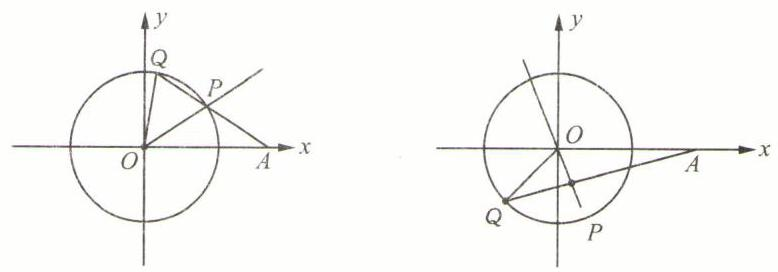
\includegraphics[width=0.6\textwidth]{bodyxb/src/bo_d20cdrf7aajc73bfmvhg_57_406_125_778_272_0.jpg}
\end{center}


[第 70(3)题]

(4)点 $C$ 与点 $A,B$ 不重合. 方法一:在 $\bigtriangleup {ABD}$ 中, $\left| {CB}\right|  = \left| {CD}\right|$ 且 $\angle {ACB} = \angle {ACD} = \dfrac{\pi }{2},\left| {AD}\right|  = \left| {AB}\right|  = 2$ . 所以, $P$ 是等腰三角形 ${ABD}$ 中线的交点,即 $P$ 是重心. 运用 70(3) 小问中的方法,可知 $\dfrac{\left| PO\right| }{\left| PD\right| } = \dfrac{1}{2}$ . 设点 $P$ 的坐标为(x, y),则 $D\left( {{3x},{3y}}\right) ,C\left( {\dfrac{{3x} + 1}{2},\dfrac{3y}{2}}\right)$ ,代入圆的方程,得 ${\left( \dfrac{{3x} + 1}{2}\right) }^{2} + {\left( \dfrac{3y}{2}\right) }^{2} = 1$ ,整理得 ${\left( x + \dfrac{1}{3}\right) }^{2} + {y}^{2} = \dfrac{4}{9}\left( {y \neq  0}\right)$ . 方法二: 记点 $C\left( {{x}_{C},{y}_{C}}\right)$ ,则 $D\left( {2{x}_{C} - 1,2{y}_{C}}\right)$ ,故 ${l}_{AC} : {y}_{C}x - \left( {{x}_{C} + 1}\right) y + {y}_{C} = 0,{l}_{OD} : 2{y}_{C}x - \left( {2{x}_{C} - 1}\right) y = 0$ ,两直线的交点为 $P\left( {\dfrac{2{x}_{C} - 1}{3},\dfrac{2{y}_{C}}{3}}\right)$ . 设点 $P$ 的坐标为(x, y),则 $C\left( {\dfrac{{3x} + 1}{2},\dfrac{3y}{2}}\right)$ ,代入圆的方程,整理得 ${\left( x + \dfrac{1}{3}\right) }^{2} + {y}^{2} =$  $\dfrac{4}{9}\left( {y \neq  0}\right)$ .

71. (1) 设点 $P$ 的坐标 $P\left( {x,y}\right)$ . 在 $\mathrm{{Rt}}\bigtriangleup {COB}$ 和 $\mathrm{{Rt}}\bigtriangleup {CAB}$ 中, ${OP}$ 和 ${AP}$ 分别是斜边 ${CB}$ 上的中线,因此有 $\left| {OP}\right|  = \left| {AP}\right|  =$  $\dfrac{1}{2}\left| {BC}\right| ,\therefore \sqrt{{x}^{2} + {y}^{2}} = \sqrt{{\left( x - a\right) }^{2} + {\left( y - b\right) }^{2}}$ ,整理得 ${2ax} + {2by} - {a}^{2} - {b}^{2} = 0$ ,是一条直线方程. 注: 满足条件的点都在直线上, 但直线上的每一点是否都满足条件呢? 答案是 “是的”, 但在 “几何法” 下可能比较难看出, 以下来说明这一点. 记点 $C\left( {0,c}\right) \left( {c \in  \mathbf{R}}\right)$ ,则 ${k}_{AC} = \dfrac{b - c}{a}$ ,由此可写出 ${l}_{AB} : a\left( {x - a}\right)  - \left( {c - b}\right) \left( {y - b}\right)  = 0$ ,与 $x$ 轴交于 $B\left( {-\dfrac{b}{a}\left( {c - b}\right)  + a,0}\right)$ . 设点 $P$ 的坐标为(x, y),则有 $\left\{  \begin{array}{l} {2x} =  - \dfrac{b}{a}\left( {c - b}\right)  + a, \\  {2y} = c, \end{array}\right.$ 整理得 ${2ax} + {2by} - {a}^{2} - {b}^{2} = 0$ . 又 $c \in$  $\mathbf{R}$ ,故直线上的每一点都能取到.

(2)如图,记弦为 ${AB}$ ,作 ${PD}\bot {AB}$ 于点 $D$ . 连接 ${PA}$ . 设点 $P$ 的坐标 $P\left( {x,y}\right)$ ,半径为 $r$ . 由圆 $P$ 与 $y$ 轴相切,知 $\left| x\right|  = r$ . 圆 $P$ 到 $x$ 轴的距离为 $d = \left| y\right|$ . 在 $\bigtriangleup {PAD}$ 中,运用勾股定理,得 ${r}^{2} - {d}^{2} = 1$ ,即 ${x}^{2} - {y}^{2} = 1$ .

\begin{center}
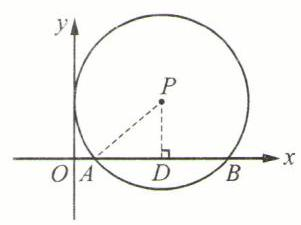
\includegraphics[width=0.2\textwidth]{bodyxb/src/bo_d20cdrf7aajc73bfmvhg_57_1144_1204_301_225_0.jpg}
\end{center}


[第 71(2)题]

(3)设点 $P$ 的坐标为(x, y),半径为 $r$ ,则圆心到两直线的距离分别为 ${d}_{1} = \dfrac{\left| 3x + y\right| }{\sqrt{10}},{d}_{2} =$  $\dfrac{\left| 3x - y\right| }{\sqrt{10}}$ . 运用几何关系: ${d}_{1}^{2} + {\left( \dfrac{8}{2}\right) }^{2} = {d}_{2}^{2} + {\left( \dfrac{4}{2}\right) }^{2} = {r}^{2}$ ,可得点 $P$ 的轨迹方程: ${xy} +$  ${10} = 0.$

(4)记圆心为 $Q$ ,设点 $P$ 的坐标为(x, y). 在 $\mathrm{{Rt}} \bigtriangleup  {APQ}$ 中运用勾股定理: ${\left| PA\right| }^{2} + {\left| PQ\right| }^{2} = {\left| AQ\right| }^{2}$ ,

$\therefore {\left( x + 3\right) }^{2} + {\left( y - 2\right) }^{2} + {\left( x - 1\right) }^{2} + {\left( y + 4\right) }^{2} = {52}$ ,整理得 ${\left( x + 1\right) }^{2} + {\left( y + 1\right) }^{2} = {13}$ (已知圆内部分).

(5)设点 $P$ 的坐标为(x, y). 在 $\mathrm{{Rt}} \bigtriangleup  {ACB}$ 中, ${CP}$ 是斜边 ${AB}$ 上的中线,因此 $\left| {PB}\right|  = \left| {PC}\right|$ .

另外,在 Rt $\bigtriangleup {OPB}$ 中运用勾股定理: ${\left| OP\right| }^{2} + {\left| PB\right| }^{2} = {\left| OB\right| }^{2},\;\therefore {\left| OP\right| }^{2} + {\left| PC\right| }^{2} = {\left| OB\right| }^{2}$ ,

$\therefore {x}^{2} + {y}^{2} + {\left( x - c\right) }^{2} + {y}^{2} = {a}^{2}$ ,整理得 ${\left( x - \dfrac{c}{2}\right) }^{2} + {y}^{2} = \dfrac{2{a}^{2} - {c}^{2}}{4}$ . 讨论: 当 $\left| c\right|  > \sqrt{2}a$ 时,点 $P$ 的轨迹不存在 (因为无法满足 $\angle {ACB} = {90}^{ \circ  }$ )；当 $\left| c\right|  = \sqrt{2}a$ 时,点 $P$ 的轨迹为一点 $\left( {\dfrac{c}{2},0}\right)$ ；当 $\left| c\right|  < \sqrt{2}a$ 时,点 $P$ 的轨迹为 ${\left( x - \dfrac{c}{2}\right) }^{2} + {y}^{2}$  $= \dfrac{2{a}^{2} - {c}^{2}}{4}$ (均在已知圆内). 注:事实上,当 $\left| c\right|  < \sqrt{2}a$ 时,圆 ${C}_{1} : {\left( x - \dfrac{c}{2}\right) }^{2} + {y}^{2} = \dfrac{2{a}^{2} - {c}^{2}}{4} = {r}_{1}^{2}$ 和圆 ${C}_{2} : {x}^{2} + {y}^{2} = {a}^{2}$  $= {r}_{2}^{2}$ 的圆心距为 $\dfrac{\left| c\right| }{2},\left| {{r}_{1} - {r}_{2}}\right|  = {r}_{2} - {r}_{1} = a - \dfrac{\sqrt{2{a}^{2} - {c}^{2}}}{2} \cdot  \dfrac{\left| c\right| }{2} < {r}_{2} - {r}_{1} \Leftrightarrow  {\left( a - \left| c\right| \right) }^{2} > 0$ ,当 $c \neq   \pm  a$ 时该不等式恒成立,因此圆 ${C}_{1}$ 内含于圆 ${C}_{2}$ .

(6)如图,连接 ${OQ}$ , ${OM}$ , ${OM}$ 与 ${AQ}$ 交于点 $F$ ；作 ${QG} \bot  {AM}$ 于点 $G$ , ${QG}$ 和 ${OM}$ 交于点 $H$ ,连接 ${AH}$ .

下证: $\left| {AH}\right|  = \left| {AO}\right| .\because {MA},{MQ}$ 均为圆 $O$ 的切线,因此 ${OA}\bot {AM},{OQ}\bot {QM}$ ,且 ${OM}$ 垂直平分 ${AQ}$ 于点 $F$ ,

$\therefore H$ 是 ${QG}$ 和 ${OM}$ 的交点,即 $\bigtriangleup {AQM}$ 的垂心.

$\therefore {QH} \bot  {AM},{AH} \bot  {QM},\therefore {OA}//{QH},{OQ}//{AH}$ ,即四边形 ${AOQH}$ 是平行四边形. 又 $\left| {OA}\right|  = \left| {OQ}\right| ,\therefore$ 四边形 ${AOQH}$ 是菱形, $\therefore \left| {AH}\right|  = \left| {AO}\right|  = 2$ ,证毕. 设点 $H$ 的坐标 $H\left( {x,y}\right)$ . 在 $\mathrm{{Rt}} \bigtriangleup  \mathrm{{HGA}}$ 中, ${\left| GA\right| }^{2} + {\left| HG\right| }^{2} = {\left| HA\right| }^{2},\therefore {x}^{2} + {\left( y - 2\right) }^{2} = 4\left( {x \neq  0}\right)$ . 注:本题用“几何法”,也较难看出满足方程的点是否均满足题意,以下说明这一点: 设 $M\left( {m,2}\right) \left( {m \neq  0}\right)$ ,则 ${l}_{OM} : y - \dfrac{m}{2}x = 0$ ; 圆 $O$ 上一点 $Q$  $\left( {{x}_{Q},{y}_{Q}}\right) \left( {{x}_{Q} \neq  0}\right)$ 的切线方程为 ${x}_{Q}x + {y}_{Q}y = 4$ ,代入 $M\left( {m,2}\right)$ ,可得 ${x}_{Q}m +$  $2{y}_{Q} = 4$ ,再代入圆 $O$ 的方程,可解得 $\left\{  {\begin{array}{l} {x}_{Q} = \dfrac{8m}{4 + {m}^{2}}, \\  {y}_{Q} = \dfrac{8 - 2{m}^{2}}{4 + {m}^{2}}. \end{array}{x}_{H} = {x}_{Q} = \dfrac{8m}{4 + {m}^{2}},{y}_{H} = }\right.$  $\dfrac{m}{2}{x}_{H} = \dfrac{4{m}^{2}}{4 + {m}^{2}}$ ,消去 $m$ ,得 ${x}^{2} + {\left( y - 2\right) }^{2} = 4.m \neq  0$ 时, $0 < \left| x\right|  \leq  2,0 < \left| y\right|  < 4$ ,可见 ${x}^{2} + {\left( y - 2\right) }^{2} = 4\left( {x \neq  0}\right)$ 上的一点确实都满足题意.

\begin{center}
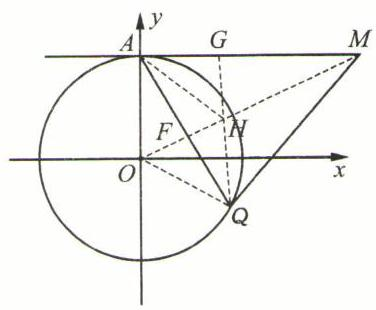
\includegraphics[width=0.3\textwidth]{bodyxb/src/bo_d20cdrf7aajc73bfmvhg_58_1116_126_376_310_0.jpg}
\end{center}


[第 71(6)题]

72. D 提示:由题意, $\sin \alpha  > 0,\cos \alpha  < 0$ . 圆心坐标为 $\left( {-\cos \alpha , - \sin \alpha }\right)$ ,其横坐标为正,纵坐标为负,故圆心在第四象限.

73. B 提示: 由题意, ${16} + m > {25} - m > 0$ ,解得 $m \in  \left( {\dfrac{9}{2},{25}}\right)$ .

74. B 提示: 椭圆在 $x$ 轴上的顶点是 $\left( {\pm 3,0}\right)$ ,圆的圆心是(a,0),半径为3,因此当 $\left| a\right|  > 6$ 时,椭圆与圆必无公共点. 当 $\left| a\right|$  $\leq  6$ 时,从图像上看,应该是有公共点的,以下严格证明:将椭圆方程变形为 ${y}^{2} = 4 - \dfrac{4{x}^{2}}{9}$ ,代入圆的方程,得 ${\left( a - x\right) }^{2} = 5$  $+ \dfrac{4}{9}{x}^{2}$ ,即 $a = x \pm  \sqrt{5 + \dfrac{4}{9}{x}^{2}}\left( {-3 \leq  x \leq  3}\right) .f\left( x\right)  = x + \sqrt{5 + \dfrac{4}{9}{x}^{2}}$ 在区间 $\left\lbrack  {0,3}\right\rbrack$ 上是严格增函数,而当 $- 3 \leq  x < 0$ 时, $f\left( x\right)  = \dfrac{5 - \dfrac{5}{9}{x}^{2}}{-x + \sqrt{5 + \dfrac{4}{9}{x}^{2}}}$ 也是严格增函数,故 $f\left( x\right)$ 的值域是 $\left\lbrack  {f\left( {-3}\right) ,f\left( 3\right) }\right\rbrack$ ,即 $\left\lbrack  {0,6}\right\rbrack$ ; 类似地,可知 $g\left( x\right)  = x -$  $\sqrt{5 + \dfrac{4}{9}{x}^{2}}\left( {-3 \leq  x \leq  3}\right)$ 的值域是 $\left\lbrack  {-6,0}\right\rbrack$ ,因此,当 $\left| a\right|  \leq  6$ 时,圆与椭圆确实都有公共点. 注:若直接联立圆与椭圆的方程,消去 $y$ ,得 $\dfrac{5}{9}{x}^{2} - {2ax} + {a}^{2} - 5 = 0\left( {}^{ * }\right)$ ,由 $\Delta  = \dfrac{16}{9}{a}^{2} + \dfrac{100}{9} > 0$ ,从而认为 $a \in  \mathbf{R}$ ,则会得到错误的答案,因为方程 (*) 不仅要有解,而且解还要满足 $- 3 \leq  x \leq  3$ ,通过解不等式,也能得到 $a \in  \left\lbrack  {-6,6}\right\rbrack$ .

75. D 提示: 由题意, $x =  \pm  c$ 与椭圆公共点的纵坐标为 $\pm  b\sqrt{1 - \dfrac{{c}^{2}}{{a}^{2}}} =  \pm  \dfrac{{b}^{2}}{a}$ ,因此所求弦长为 $\dfrac{2{b}^{2}}{a}$ .

76. $C$ 提示:椭圆焦点 ${F}_{2}\left( {c,0}\right)$ 到直线 $x = \dfrac{{a}^{2}}{c}$ 的距离为 $\dfrac{{a}^{2}}{c} - c = \dfrac{{b}^{2}}{c}$ ,由题意, $\dfrac{{b}^{2}}{c} = c,\therefore b = c$ . 记任意一焦点为 $C$ ,椭圆中心为 $O$ 短轴两端点为 $A,B$ ,则 $\angle {COA} = \angle {COB} = \dfrac{\pi }{2}$ ,又 $\left| {OA}\right|  = \left| {OB}\right|  = \left| {OC}\right|$ ,因此 $\angle {ACB} = \dfrac{\pi }{2}$ .

77. B 提示: 由题意, ${\left( m - 1\right) }^{2} > {m}^{2} > 0$ ,解得 $m < \dfrac{1}{2}$ 且 $m \neq  0$ .

78. $C$ 提示:由题意, $\dfrac{2{a}^{2}}{c} = 3 \cdot  {2c}$ , $\therefore \;e = \dfrac{c}{a} = \dfrac{\sqrt{3}}{3}$ .

79. B 提示: $\left| {AB}\right|  = \left| {A{F}_{1}}\right|  + \left| {B{F}_{1}}\right|$ ,利用椭圆的定义,可得 $\bigtriangleup {AB}{F}_{2}$ 的周长为 $C = \left| {AB}\right|  + \left| {A{F}_{2}}\right|  + \left| {B{F}_{2}}\right|  =$  $\left| {A{F}_{1}}\right|  + \left| {A{F}_{2}}\right|  + \left| {B{F}_{1}}\right|  + \left| {B{F}_{2}}\right|  = 2 \cdot  {2a} = {4a}.$

80. B

81. $D$ 提示:由题意, ${a}^{2} = \dfrac{1}{k},{b}^{2} = \dfrac{1}{3k},\;\therefore \;{c}^{2} = {a}^{2} - {b}^{2} = \dfrac{2}{3k} = {16}$ ,解得 $k = \dfrac{1}{24}$ .

82. (1) $3 < k < 5$ 且 $k \neq  4$ 提示: 将方程整理得 $\dfrac{{x}^{2}}{5 - k} + \dfrac{{y}^{2}}{k - 3} = 1$ ,由题意, $5 - k > 0$ 且 $k - 3 > 0$ 且 $5 - k \neq  k - 3$ ,

$\therefore 3 < k < 5$ 且 $k \neq  4$ .

(2) $\left( {\dfrac{\pi }{2},\dfrac{3\pi }{4}}\right)$ 提示:由题意, $- \dfrac{1}{\cos \alpha } > \dfrac{1}{\sin \alpha } > 0$ ,等价于不等式组 $\left\{  \begin{array}{l} \sin \alpha  > 0, \\  \tan \alpha  <  - 1, \end{array}\right.$ 又 $0 \leq  \alpha  < {2\pi }$ ,故 $\alpha  \in  \left( {\dfrac{\pi }{2},\dfrac{3\pi }{4}}\right)$ .

83. (1) $\dfrac{3}{5}$ 提示:由题意: ${2b} = a + c$ ,又 ${a}^{2} - {c}^{2} = {b}^{2}$ ,可得 $\left\{  {\begin{array}{l} a + c = {2b}, \\  a - c = \dfrac{b}{2}, \end{array}\therefore \left\{  {\begin{array}{l} a = \dfrac{5}{4}b, \\  c = \dfrac{3}{4}b, \end{array}\therefore \;e = \dfrac{c}{a} = \dfrac{3}{5}}\right. }\right.$ .

(2) $\sqrt{3} - 1$ 提示:记椭圆的焦点为 ${F}_{1},{F}_{2}$ ,椭圆与圆的中心都在 $O$ ,椭圆与圆的任意一个公共点为 $A$ (位于第二象限), 圆的半径为 $r$ . 由题意, $\angle {F}_{1}{OA} = \dfrac{1}{6} \cdot  {2\pi } = \dfrac{\pi }{3}$ ,因此 $\bigtriangleup {F}_{1}{OA}$ 是等边三角形,故 $c = \left| {O{F}_{1}}\right|  = \left| {A{F}_{1}}\right|  = r;\operatorname{Rt}\bigtriangleup {F}_{1}A{F}_{2}$ 中, $\angle {F}_{1}A{F}_{2} = \dfrac{\pi }{2}$ ,不难得到 $\left| {A{F}_{2}}\right|  = \sqrt{3}r.\;\therefore \;{2a} = \left| {A{F}_{1}}\right|  + \left| {A{F}_{2}}\right|  = \left( {1 + \sqrt{3}}\right) r,\;\therefore \;e = \dfrac{c}{a} = \sqrt{3} - 1$ .

3 $\sqrt{3} - 1$ 提示:由题意, $\angle P{F}_{1}{F}_{2} = {30}^{ \circ  },\angle P{F}_{2}{F}_{1} = {60}^{ \circ  },\angle {F}_{1}P{F}_{2} = {90}^{ \circ  }$ . 若 $\left| {{F}_{1}{F}_{2}}\right|  = {2c}$ ,则 ${2a} = \left| {P{F}_{1}}\right|  + \left| {P{F}_{2}}\right|  =$  $\sqrt{3}c + c,\;\therefore \;e = \dfrac{c}{a} = \sqrt{3} - 1.$

84. (1) $\dfrac{{x}^{2}}{9} + {y}^{2} = 1$ 或 $\dfrac{{x}^{2}}{9} + \dfrac{{y}^{2}}{81} = 1$ 提示: 若椭圆焦点在 $x$ 轴上,设椭圆方程为 $\dfrac{{x}^{2}}{{\left( 3b\right) }^{2}} + \dfrac{{y}^{2}}{{b}^{2}} = 1$ ,代入 $P\left( {3,0}\right)$ ,得 ${b}^{2} = 1$ ; 若椭圆焦点在 $y$ 轴上,设椭圆方程为 $\dfrac{{x}^{2}}{{b}^{2}} + \dfrac{{y}^{2}}{{\left( 3b\right) }^{2}} = 1$ ,代入 $P\left( {3,0}\right)$ ,得 ${b}^{2} = 9$ . 因此,所求椭圆方程为 $\dfrac{{x}^{2}}{9} + {y}^{2} = 1$ 或 $\dfrac{{x}^{2}}{9} + \dfrac{{y}^{2}}{81}$  $= 1$ .

(2) $\dfrac{{x}^{2}}{25} + \dfrac{{y}^{2}}{9} = 1$ 或 $\dfrac{{x}^{2}}{16} + \dfrac{{y}^{2}}{25} = 1$ 提示:直线与坐标轴的交点为:(4,0) 和 (0,3). 若(4,0)为焦点(焦点在 $x$ 轴上),则 $c = 4$ , $b = 3$ ,故 $a = \sqrt{{b}^{2} + {c}^{2}} = 5$ ,椭圆方程为 $\dfrac{{x}^{2}}{25} + \dfrac{{y}^{2}}{9} = 1$ ; 若(0,3)为焦点 (焦点在 $y$ 轴上),则 $c = 3,b = 4$ ,故 $a = \sqrt{{b}^{2} + {c}^{2}}$  $= 5$ ,椭圆方程为 $\dfrac{{x}^{2}}{16} + \dfrac{{y}^{2}}{25} = 1$ .

(3) $\dfrac{{x}^{2}}{16} + \dfrac{{y}^{2}}{7} = 1$ 或 $\dfrac{{x}^{2}}{7} + \dfrac{{y}^{2}}{16} = 1$ 提示: 由题意 $\left\{  \begin{array}{l} {2a} = 7 + 1, \\  {2c} = 7 - 1, \end{array}\right.$ 故 $\left\{  \begin{array}{l} a = 4, \\  c = 3, \end{array}\right. \therefore {b}^{2} = {a}^{2} - {c}^{2} = 7$ ,因此所求椭圆方程为 $\dfrac{{x}^{2}}{16} + \dfrac{{y}^{2}}{7} = 1$ 或 $\dfrac{{x}^{2}}{7} + \dfrac{{y}^{2}}{16} = 1$ .

(4) $\dfrac{{x}^{2}}{12} + \dfrac{{y}^{2}}{3} = 1$ 或 $\dfrac{{x}^{2}}{3} + \dfrac{{y}^{2}}{12} = 1$ 提示: 由题意 $\left\{  \begin{array}{l} a = {2b}, \\  \dfrac{{a}^{2}}{c} = 4, \\  {a}^{2} = {b}^{2} + {c}^{2}, \end{array}\right.$ 解得 $\left\{  \begin{array}{l} a = 2\sqrt{3}, \\  b = \sqrt{3}, \\  c = 3, \end{array}\right.$ 因此椭圆方程为 $\dfrac{{x}^{2}}{12} + \dfrac{{y}^{2}}{3} = 1$ 或 $\dfrac{{x}^{2}}{3} + \dfrac{{y}^{2}}{12} = 1$ .

(5) $\dfrac{{x}^{2}}{5} + \dfrac{{y}^{2}}{\dfrac{20}{9}} = 1$ 提示: 由题意 $\left\{  \begin{array}{l} e = \dfrac{c}{a} = \dfrac{\sqrt{5}}{3}, \\  \dfrac{{a}^{2}}{c} = 3, \end{array}\right.$ 解得 $\left\{  \begin{array}{l} a = \sqrt{5}, \\  c = \dfrac{5}{3}, \end{array}\right. {b}^{2} = {a}^{2} - {c}^{2} = \dfrac{20}{9}$ ,因此椭圆方程为 $\dfrac{{x}^{2}}{5} + \dfrac{{y}^{2}}{\dfrac{20}{9}} = 1$ .

(6) $\dfrac{{x}^{2}}{\dfrac{25}{4}} + \dfrac{{y}^{2}}{4} = 1$ 提示: 由题意 $\left\{  \begin{array}{l} a - c = 1, \\  \dfrac{{a}^{2}}{c} - a = \dfrac{5}{3}, \end{array}\right.$ 解得 $\left\{  \begin{array}{l} a = \dfrac{5}{2}, \\  c = \dfrac{3}{2}, \end{array}\right. {b}^{2} = {a}^{2} - {c}^{2} = 4$ ,因此椭圆方程为: $\dfrac{{x}^{2}}{\dfrac{25}{4}} + \dfrac{{y}^{2}}{4} = 1$ .

85. B 提示: $a = {10}$ ,点 $P$ 到右焦点的距离是 8 ,故点 $P$ 到左焦点的距离为 ${20} - 8 = {12}$ .

86. A 提示:椭圆的标准方程为 $\dfrac{{x}^{2}}{-b} + \dfrac{{y}^{2}}{-a} = 1$ ,由题意, $- b >  - a > 0$ ,因此焦点在 $x$ 轴上, $c = \sqrt{-b - \left( {-a}\right) } = \sqrt{a - b}$ ,故焦点坐标为 $\left( {\pm \sqrt{a - b},0}\right)$ .

87. $B$ 提示:点 $P$ 的坐标为 $\left( {-c, \pm  \dfrac{{b}^{2}}{a}}\right)$ ,因此点 $P$ 到左焦点的距离 $\left| {P{F}_{1}}\right|  = \dfrac{{b}^{2}}{a}$ . 由题意, ${\left| {F}_{1}{B}_{2}\right| }^{2} = \left| {O{F}_{1}}\right|  \cdot  \left| {{B}_{1}{B}_{2}}\right|  = c$ . ${2b}$ ；另外,在 $\mathrm{{Rt}} \bigtriangleup  {F}_{1}O{B}_{2}$ 中,由勾股定理得 ${\left| {F}_{1}{B}_{2}\right| }^{2} = {\left| O{F}_{1}\right| }^{2} + {\left| O{B}_{2}\right| }^{2} = {c}^{2} + {b}^{2},\;\therefore \;b = c,a = \sqrt{{b}^{2} + {c}^{2}} = \sqrt{2}b$ , $\therefore \dfrac{\left| P{F}_{1}\right| }{\left| O{B}_{2}\right| } = \dfrac{b}{a} = \dfrac{\sqrt{2}}{2}$ .

88. (1) 设 $P\left( {x,y}\right)$ ,椭圆的焦点为 ${F}_{1}\left( {-4,0}\right) ,{F}_{2}\left( {4,0}\right)$ ,则 $\vv{{F}_{1}P} = \left( {x + 4,y}\right) ,\vv{{F}_{2}P} = \left( {x - 4,y}\right)$ ,由题意, $\vv{{F}_{1}P} \cdot  \vv{{F}_{2}P} = {x}^{2} -$  ${16} + {y}^{2} = 0$ (注意到,这就是以 ${F}_{1}{F}_{2}$ 为直径的圆). 联立 $\left\{  \begin{array}{l} {x}^{2} + {y}^{2} = {16}, \\  \dfrac{{x}^{2}}{25} + \dfrac{{y}^{2}}{9} = 1, \end{array}\right.$ 解得点 $P$ 的坐标为 $\left( {\dfrac{5\sqrt{7}}{4},\dfrac{9}{4}}\right) ,\left( {-\dfrac{5\sqrt{7}}{4},\dfrac{9}{4}}\right)$ , $\left( {\dfrac{5\sqrt{7}}{4}, - \dfrac{9}{4}}\right) ,\left( {-\dfrac{5\sqrt{7}}{4}, - \dfrac{9}{4}}\right)$ .

(2)长轴两顶点到右焦点的距离分别为 $a + c$ 和 $a - c$ ,因此点 $P$ 到右焦点的距离为 $a$ ,设 $P\left( {x,y}\right)$ ,联立 $\left\{  \begin{array}{l} {\left( x - \sqrt{5}\right) }^{2} + {y}^{2} = 9, \\  \dfrac{{x}^{2}}{9} + \dfrac{{y}^{2}}{4} = 1, \end{array}\right.$ 可得点 $P$ 的坐标为(0,2)或(0, - 2).

89. (1) 由题意, ${2a} = {6.5} + {3.5},\;\therefore a = 5$ . 若椭圆左右焦点分别为 ${F}_{1}\left( {-c,0}\right)$ 和 ${F}_{2}\left( {c,0}\right)$ ,则 $\left\{  \begin{array}{l} \left| {P{F}_{1}}\right|  = {\left( 3 + c\right) }^{2} + {y}^{2} = {6.5}^{2}, \\  \left| {P{F}_{2}}\right|  = {\left( 3 - c\right) }^{2} + {y}^{2} = {3.5}^{2}, \end{array}\right.$ 消去 $y$ ,可得 $c = \dfrac{5}{2},\;\therefore \;{b}^{2} = {a}^{2} - {c}^{2} = \dfrac{75}{4},\;\therefore$ 椭圆方程为 $\dfrac{{x}^{2}}{25} + \dfrac{4{y}^{2}}{75} = 1$ .

(2) $a = 3\sqrt{5},b = 2\sqrt{5},c = 5$ . 设 $P\left( {x,y}\right) \left( {x,y > 0}\right)$ ,椭圆的焦点为 ${F}_{1}\left( {-5,0}\right) ,{F}_{2}\left( {5,0}\right)$ ,则 $\vv{{F}_{1}P} = \left( {x + 5,y}\right) ,\vv{{F}_{2}P} =$ (x - 5, y),由题意, $\vv{{F}_{1}P} \cdot  \vv{{F}_{2}P} = {x}^{2} - {25} + {y}^{2} = 0$ (注意到,这就是以 ${F}_{1}{F}_{2}$ 为直径的圆). 联立 $\left\{  \begin{array}{l} {x}^{2} + {y}^{2} = {25}, \\  \dfrac{{x}^{2}}{45} + \dfrac{{y}^{2}}{20} = 1, \end{array}\right.$ 解得点 $P$ 的坐标为(3,4).

90. 设定点 $A\left( {a,0}\right) \left( {a > 0}\right)$ ,则直线方程为 $l : y = x - a$ . 代入椭圆方程,整理得 $3{x}^{2} - {4ax} + 2{a}^{2} - {12} = 0,\Delta  = {144} - 8{a}^{2}$ . 直线 $l$ 被椭圆截得的弦长为 $\dfrac{\sqrt{1 + {k}_{i}^{2}}\sqrt{\Delta }}{3} = \dfrac{4}{3}\sqrt{{18} - {a}^{2}} = \dfrac{4}{3}\sqrt{14},$ 又 $a > 0,\therefore a = 2$ ,点 $A$ 的坐标为 $A\left( {2,0}\right)$ .

91. D 提示: 不妨设 $F$ 是左焦点,则 $F\left( {-c,0}\right)$ . 弦 ${PQ}$ 的斜率为 0 时, $P,Q,F$ 三点不能构成三角形,因此设 ${l}_{PQ} : x - {ky} = 0$ , 代入椭圆方程,得 ${y}^{2} = \dfrac{{a}^{2}{b}^{2}}{{a}^{2} + {b}^{2}{k}^{2}}$ . $\left| {PQ}\right|  = 2\left| {OP}\right|  = 2\sqrt{{x}_{P}^{2} + {y}_{P}^{2}} = 2\sqrt{1 + {k}^{2}}\left| {y}_{P}\right|  = 2\sqrt{1 + {k}^{2}}\dfrac{ab}{\sqrt{{a}^{2} + {b}^{2}{k}^{2}}}$ ; 点 $F$ 到直线 ${PQ}$ 的距离为 $h = \dfrac{\left| -c\right| }{\sqrt{1 + {k}^{2}}}$ . $\therefore {S}_{\bigtriangleup {PQF}} = \dfrac{1}{2}\left| {PQ}\right|  \cdot  h = \dfrac{abc}{\sqrt{{a}^{2} + {b}^{2}{k}^{2}}} \leq  \dfrac{abc}{a} = {bc}$ ,当且仅当 $k = 0$ 时等号成立. 因此, $\bigtriangleup {PQF}$ 的面积最大为 ${bc}$ ,此时弦 ${PQ}$ 即为椭圆的短轴.

92. $C$ 提示:直线过定点 $A\left( {0,1}\right)$ ,斜率为 $k.a \geq  1$ 时,点 $A$ 在椭圆上或椭圆内,因此直线与椭圆必有公共点； $0 < a < 1$ 时,取 $k = 0$ ,此时直线 $y = 1$ 与椭圆无公共点. 又焦点在 $x$ 轴上,故 ${a}^{2} < {49}$ . 综上, $1 \leq  a < 7$ .

93. D 提示: 在 $\bigtriangleup M{F}_{1}{F}_{2}$ 中,设 $\left| {M{F}_{1}}\right|  = x$ ,则 $\left| {M{F}_{2}}\right|  = {2a} - x,\alpha  \neq  0$ ,运用正弦定理: $\dfrac{x}{\sin \alpha } = \dfrac{{2a} - x}{\sin {2\alpha }} = \dfrac{2c}{\sin \left( {\pi  - {3\alpha }}\right) }$ . 由 $\dfrac{x}{\sin \alpha } =$  $\dfrac{{2a} - x}{\sin {2\alpha }}$ ,可得 $x = \dfrac{2a}{2\cos \alpha  + 1}$ ; 由 $\dfrac{x}{\sin \alpha } = \dfrac{2c}{\sin \left( {\pi  - {3\alpha }}\right) }$ ,可得 $e = \dfrac{c}{a} = \dfrac{\sin {3\alpha }}{\sin \alpha  \cdot  \left( {2\cos \alpha  + 1}\right) }$ . 其中 $\sin {3\alpha } = \sin {2\alpha }\cos \alpha  + \cos {2\alpha }\sin \alpha  =$  $\sin \alpha \left( {4{\cos }^{2}\alpha  - 1}\right)  = \sin \alpha \left( {2\cos \alpha  + 1}\right) \left( {2\cos \alpha  - 1}\right)$ ,故椭圆的离心率 $e = 2\cos \alpha  - 1$ .

94. A 提示: 在 $\mathrm{{Rt}} \bigtriangleup  M{F}_{1}{F}_{2}$ 中, $\left| {{F}_{1}{F}_{2}}\right|  = {2c},\left| {M{F}_{2}}\right|  = c$ ,则 $\left| {M{F}_{1}}\right|  = {2a} - c,\angle {F}_{1}M{F}_{2} = \dfrac{\pi }{2}$ ,运用勾股定理,得 ${\left( 2a - c\right) }^{2} +$  ${c}^{2} = {\left( 2c\right) }^{2}$ ,解得 $c = \left( {\sqrt{3} - 1}\right) a$ ,故 $e = \dfrac{c}{a} = \sqrt{3} - 1$ .

95. 由题意, $a = 3,c = \sqrt{9 - 5} = 2$ ,记椭圆右焦点 ${F}_{2}\left( {2,0}\right) .\left| {PA}\right|  + \left| {P{F}_{1}}\right|  = \left| {PA}\right|  + {2a} - \left| {P{F}_{2}}\right|  = 6 + \left| {PA}\right|  - \left| {P{F}_{2}}\right|  \leq  6 +$  $\left| {A{F}_{2}}\right|  = 6 + \sqrt{2}$ ,此时点 $P$ 是直线 $A{F}_{2}$ 与椭圆在第四象限的公共点 $P\left( {\dfrac{{18} + {15}\sqrt{2}}{14},\dfrac{{10} - {15}\sqrt{2}}{14}}\right)$ .

96. (1) 由题意, $a = 3,c = \sqrt{9 - 4} = \sqrt{5}$ ,设 $\left| {P{F}_{1}}\right|  = x$ ,则 $\left| {P{F}_{2}}\right|  = {2a} - x = 6 - x$ . 在 $\operatorname{Rt} \bigtriangleup  {F}_{1}P{F}_{2}$ 中运用勾股定理,得 ${x}^{2} +$  ${\left( 6 - x\right) }^{2} = {\left( 2\sqrt{5}\right) }^{2},{6}^{2} = {\left( x + 6 - x\right) }^{2} = {x}^{2} + {\left( 6 - x\right) }^{2} + {2x}\left( {6 - x}\right)  = {20} + {2x}\left( {6 - x}\right) ,\;\therefore \;{2x}\left( {6 - x}\right)  = {16}$ , ${S}_{\bigtriangleup {F}_{1}P{F}_{2}} = \dfrac{1}{2}x\left( {6 - x}\right)  = 4.$

(2)证明:设 $\left| {P{F}_{1}}\right|  = x$ ,则 $\left| {P{F}_{2}}\right|  = {2a} - x$ . 在 $\bigtriangleup {F}_{1}P{F}_{2}$ 中使用余弦定理,可得 ${x}^{2} + {\left( 2a - x\right) }^{2} - {2x}\left( {{2a} - x}\right) \cos \theta  =$  ${\left( 2c\right) }^{2}$ . 运用 (1) 的技巧: 代入: ${x}^{2} + {\left( 2a - x\right) }^{2} = {\left( 2a\right) }^{2} - {2x}\left( {{2a} - x}\right)$ ,得 $x\left( {{2a} - x}\right) \left( {1 + \cos \theta }\right)  = 2\left( {{a}^{2} - {c}^{2}}\right)  = 2{b}^{2}$ . 又 $0 < \theta  < \pi$ ,故 ${S}_{\bigtriangleup {F}_{1}P{F}_{2}} = \dfrac{1}{2}x\left( {{2a} - x}\right) \sin \theta  = \dfrac{\sin \theta }{1 + \cos \theta }{b}^{2} = {b}^{2}\tan \dfrac{\theta }{2}$ ,证毕.

97. (1) $\sqrt{{\left( {x}_{0} \pm  c\right) }^{2} + {y}_{0}^{2}} = \sqrt{{\left( {x}_{0} \pm  c\right) }^{2} + {b}^{2}\left( {1 - \dfrac{{x}^{2}}{{a}^{2}}}\right) } = \sqrt{\dfrac{{c}^{2}}{{a}^{2}}{x}_{0}^{2} \pm  {2c}{x}_{0} + {a}^{2}} = \sqrt{{\left( a \pm  e{x}_{0}\right) }^{2}} = a \pm  e{x}_{0}$ . 故点 $P$ 到椭圆的左、 右焦点的距离是 $a \pm  e{x}_{0}$ ,证毕.

(2)记 $\left| {P{F}_{1}}\right|  = x$ ,则 $\left| {P{F}_{2}}\right|  = {2a} - x$ . $\left| {P{F}_{1}}\right|  \cdot  \left| {P{F}_{2}}\right|  = x\left( {{2a} - x}\right)  =  - {\left( x - a\right) }^{2} + {a}^{2}$ . 根据( 1 )的结论,若点 $P$ 的横坐标是 ${x}_{0}$ ,则 $\left| {P{F}_{1}}\right|  = x = a + e{x}_{0},{x}_{0} \in  \left\lbrack  {-a,a}\right\rbrack  ,\;\therefore \;\left( {x - a}\right)  \in  \left\lbrack  {-c,c}\right\rbrack$ ,

$\therefore \left| {P{F}_{1}}\right|  \cdot  \left| {P{F}_{2}}\right|$ 的值域是 $\left\lbrack  {-{c}^{2} + {a}^{2},{a}^{2}}\right\rbrack$ ,即 $\left\lbrack  {{b}^{2},{a}^{2}}\right\rbrack$ (当点 $P$ 为椭圆的长轴端点时, $\left| {P{F}_{1}}\right|  \cdot  \left| {P{F}_{2}}\right|$ 取到最小值 ${b}^{2}$ ; 当点 $P$ 为椭圆的短轴端点时, $\left| {P{F}_{1}}\right|  \cdot  \left| {P{F}_{2}}\right|$ 取到最大值 ${a}^{2}$ ),证毕.

(3)设椭圆上三点的横坐标为 ${x}_{1},{x}_{2},{x}_{3}$ ,由(1)知:它们到椭圆的左、右焦点的距离是: $a \pm  e{x}_{1}$ , $a \pm  e{x}_{2}$ , $a \pm  e{x}_{3}$ . 充分性: 若椭圆上三点的横坐标 ${x}_{1},{x}_{2},{x}_{3}$ 成等差数列,则 $2{x}_{2} = {x}_{1} + {x}_{3}$ ,

$\therefore 2\left( {a \pm  e{x}_{2}}\right)  = \left( {a \pm  e{x}_{1}}\right)  + \left( {a \pm  e{x}_{3}}\right)$ ,即这三点的焦半径也成等差数列. 必要性: 若三点的焦半径成等差数列, 则 $2\left( {a \pm  e{x}_{2}}\right)  = \left( {a \pm  e{x}_{1}}\right)  + \left( {a \pm  e{x}_{3}}\right) ,\therefore 2{x}_{2} = {x}_{1} + {x}_{3}$ ,即这三点的横坐标也成等差数列. 证毕.

98. (1) 设 $A\left( {{x}_{1},{y}_{1}}\right) ,B\left( {{x}_{2},{y}_{2}}\right) \left( {{x}_{1} \neq  {x}_{2}}\right)$ ,则有 $4{x}_{1}^{2} + 9{y}_{1}^{2} = {36},4{x}_{2}^{2} + 9{y}_{2}^{2} = {36}$ ,两式相减,并代入 $\dfrac{{x}_{1} + {x}_{2}}{2} = 1$ 和 $\dfrac{{y}_{1} + {y}_{2}}{2} = 1$ ,

$\therefore {k}_{AB} = \dfrac{{y}_{1} - {y}_{2}}{{x}_{1} - {x}_{2}} =  - \dfrac{4}{9},\;\therefore {l}_{AB} : y - 1 =  - \dfrac{4}{9}\left( {x - 1}\right)$ ,即 ${4x} + {9y} - {13} = 0$ .

(2)将椭圆方程写为 $4{x}^{2} + {y}^{2} = 4$ . 方法一:将 $y = {2x} + m$ 代入椭圆方程,整理得 $8{x}^{2} + {4mx} + {m}^{2} - 4 = 0,\Delta  = {128} - {16}{m}^{2}$  $> 0 \Rightarrow   - 2\sqrt{2} < m < 2\sqrt{2}$ ,此时 ${x}_{1} + {x}_{2} =  - \dfrac{4m}{8} =  - \dfrac{m}{2}$ . 记所连线段的中点为 $\left( {{x}_{M},{y}_{M}}\right)$ ,则 ${x}_{M} = \dfrac{{x}_{1} + {x}_{2}}{2} =  - \dfrac{m}{4}$ ,代入 $y = {2x} + m$ ,得 ${y}_{M} = \dfrac{m}{2}$ ,消去参数 $m$ ,可得所连线段的轨迹方程为 ${2x} + y = 0\left( {-\dfrac{\sqrt{2}}{2} < x < \dfrac{\sqrt{2}}{2}}\right)$ . 方法二: (点差法) 记所连线段的两端点为 $A\left( {{x}_{1},{y}_{1}}\right) ,B\left( {{x}_{2},{y}_{2}}\right) \left( {{x}_{1} \neq  {x}_{2}}\right)$ ,所连线段的中点为 $\left( {{x}_{M},{y}_{M}}\right)$ ,则有 $4{x}_{1}^{2} + {y}_{1}^{2} = 4,4{x}_{2}^{2} + {y}_{2}^{2} = 4$ , 两式相减,并除以 ${x}_{1} - {x}_{2}$ ,得 $4\left( {{x}_{1} + {x}_{2}}\right)  + \left( {{y}_{1} + {y}_{2}}\right) \dfrac{{y}_{1} - {y}_{2}}{{x}_{1} - {x}_{2}} = 0$ . 其中, ${x}_{1} + {x}_{2} = 2{x}_{M},{y}_{1} + {y}_{2} = 2{y}_{M},\dfrac{{y}_{1} - {y}_{2}}{{x}_{1} - {x}_{2}} = 2$ , $\therefore 8{x}_{M} + 4{y}_{M} = 0,\therefore$ 所连线段的轨迹方程为 ${2x} + y = 0$ (在椭圆内的部分,即 $- \dfrac{\sqrt{2}}{2} < x < \dfrac{\sqrt{2}}{2}$ ).

(3)将椭圆方程写为 $9{x}^{2} + {25}{y}^{2} = {225}$ . 记弦的两端点为 $P\left( {{x}_{1},{y}_{1}}\right) ,Q\left( {{x}_{2},{y}_{2}}\right) \left( {{x}_{1} \neq  {x}_{2}}\right)$ ,弦的中点为 $M\left( {{x}_{M},{y}_{M}}\right)$ ,则有 $\left\{  \begin{array}{l} 9{x}_{1}^{2} + {25}{y}_{1}^{2} = {225}, \\  9{x}_{2}^{2} + {25}{y}_{2}^{2} = {225}, \end{array}\right.$ 两式相减,并除以 ${x}_{1} - {x}_{2}$ ,得 $9\left( {{x}_{1} + {x}_{2}}\right)  + {25}\left( {{y}_{1} + {y}_{2}}\right) \dfrac{{y}_{1} - {y}_{2}}{{x}_{1} - {x}_{2}} = 0$ . 其中, ${x}_{1} + {x}_{2} = 2{x}_{M},{y}_{1} + {y}_{2}$  $= 2{y}_{M},\dfrac{{y}_{1} - {y}_{2}}{{x}_{1} - {x}_{2}} = {k}_{PQ} = \dfrac{{y}_{M} - 1}{{x}_{M} - 8},$

$\therefore {18}{x}_{M} + {50}{y}_{M}\dfrac{{y}_{M} - 1}{{x}_{M} - 8} = 0$ ,整理得中点 $M$ 的轨迹方程: $9{x}^{2} + {25}{y}^{2} - {72x} - {25y} = 0$ (已知椭圆内的部分). 注:轨迹方程可整理为 $\dfrac{{\left( x - 4\right) }^{2}}{\dfrac{601}{36}} + \dfrac{{\left( y - \dfrac{1}{2}\right) }^{2}}{\dfrac{601}{100}} = 1$ ,是一个中心在 $\left( {4,\dfrac{1}{2}}\right)$ ,长轴平行于 $x$ 轴的椭圆的一部分.

99. (1) 由题意, $\left| {AB}\right|  + \left| {AC}\right|  = 2\left| {BC}\right|  = 4$ ,可见顶点 $A$ 的轨迹是一个椭圆的一部分,且 $c = 1,{2a} = 4 \Rightarrow  a = 2,\therefore {b}^{2} =$  ${a}^{2} - {c}^{2} = 3,\therefore$ 顶点 $A$ 的轨迹方程为 $\dfrac{{x}^{2}}{4} + \dfrac{{y}^{2}}{3} = 1\left( {x > 0\text{ 且 }y \neq  0}\right)$ . 注: 根据第 97(1) 题的结论, $\left| {AB}\right|  > \left| {AC}\right|  \Leftrightarrow  a +$  $e{x}_{A} > a - e{x}_{A} \Leftrightarrow  {x}_{A} > 0$ .

(2)记 ${AB},{AC}$ 的中点分别为 $D,E$ . 根据重心的性质, $\left| {GB}\right|  + \left| {GC}\right|  = \dfrac{2}{3}\left( {\left| {BE}\right|  + \left| {CD}\right| }\right)  = {20}$ ,可见重心 $G$ 的轨迹是一个椭圆 (记椭圆 1) 的一部分,且 ${c}_{1} = 8,2{a}_{1} = {20} \Rightarrow  {a}_{1} = {10},\therefore {b}_{1} = 6,\therefore$ 重心 $G$ 的轨迹方程为 $\dfrac{{x}^{2}}{100} + \dfrac{{y}^{2}}{36} = 1(y$  $\neq  0)$ . 原点 $O$ 是 ${BC}$ 边的中点,再根据重心的性质, $\vv{OA} = 3 \cdot  \vv{OG},\;\therefore \left\{  \begin{array}{l} {x}_{G} = \dfrac{{x}_{A}}{3}, \\  {y}_{G} = \dfrac{{y}_{A}}{3}, \end{array}\right.$ 代入重心 $G$ 的轨迹方程,可得顶点 $A$ 的轨迹方程为 $\dfrac{{x}^{2}}{900} + \dfrac{{y}^{2}}{324} = 1\left( {y \neq  0}\right)$ .

(3)记定圆为圆 $G$ (圆心 $G\left( {0, - 4}\right)$ ),由题意, $\left| {PG}\right|  = \left| {\left| {PF}\right|  - {10}}\right|$ . 由于定点 $F$ 在定圆 (记为圆 $G$ ) 内部,因此动圆 $P -$ 定在定圆 $G$ 的内部, $\therefore \left| {PG}\right|  = {10} - \left| {PF}\right|$ ,即 $\left| {PG}\right|  + \left| {PF}\right|  = {10},\therefore$ 点 $P$ 的轨迹是一个椭圆 (焦点在 $y$ 轴上),且 $c = 4,{2a} = {10} \Rightarrow  a = 5,\therefore {b}^{2} = {a}^{2} - {c}^{2} = 9,\therefore$ 动圆圆心 $P$ 的轨迹方程为 $\dfrac{{x}^{2}}{9} + \dfrac{{y}^{2}}{25} = 1$ .

(4)记该椭圆的另一个焦点为 $G$ ,则 $\left| {OF}\right|  + \left| {OG}\right|  = {2a} = 4$ ,其中 $\left| {OF}\right|  = 1$ , $\therefore \left| {OG}\right|  = 3$ , $\therefore$ 点 $G$ 的轨迹方程为 ${x}^{2} + {y}^{2} = 9\left( {x \neq   - 3}\right)$ . 记椭圆的中心为 $M\left( {{x}_{M},{y}_{M}}\right)$ ,它是线段 ${FG}$ 的中点,因此 $\left\{  \begin{array}{l} {x}_{G} = 2{x}_{M} - 1, \\  {y}_{G} = 2{y}_{M}, \end{array}\right.$ 代入 ${x}^{2} + {y}^{2} = 9$ ,整理得椭圆中心的轨迹方程: ${\left( x - \dfrac{1}{2}\right) }^{2} + {y}^{2} = \dfrac{9}{4}\left( {x \neq   - 1}\right)$ .

(5) 设 $C\left( {{x}_{1},\sqrt{3}{x}_{1}}\right) ,D\left( {{x}_{2}, - \sqrt{3}{x}_{2}}\right) \left( {{x}_{1},{x}_{2} > 0}\right) ,M\left( {{x}_{M},{y}_{M}}\right) ,\left\{  \begin{array}{l} 2{x}_{M} = {x}_{1} + {x}_{2}, \\  2{y}_{M} = \sqrt{3}\left( {{x}_{1} - {x}_{2}}\right) . \end{array}\right.$ 由题意, $\left| {CD}\right|  =$  $\sqrt{{\left( {x}_{1} - {x}_{2}\right) }^{2} + 3{\left( {x}_{1} + {x}_{2}\right) }^{2}} = 4\sqrt{3}$ ,即 $\sqrt{\dfrac{4}{3}{y}_{M}^{2} + {12}{x}_{M}^{2}} = 4\sqrt{3}$ ,整理得点 $M$ 的轨迹方程为 $\dfrac{{x}^{2}}{4} + \dfrac{{y}^{2}}{36} = 1$ (夹在 $\angle {AOB}$ 内的椭圆的一段弧).

(6) 设动点坐标为(x, y),则 $\dfrac{\sqrt{{x}^{2} + {\left( y - \sqrt{7}\right) }^{2}}}{\left| y - \dfrac{{16}\sqrt{7}}{7}\right| } = \dfrac{\sqrt{7}}{4}$ . 故动点轨迹方程为 $\dfrac{{x}^{2}}{9} + \dfrac{{y}^{2}}{16} = 1$ .

100. (1) 设 $B\left( {{x}_{1},{y}_{1}}\right) ,C\left( {{x}_{2},{y}_{2}}\right) \left( {{x}_{1} \neq  {x}_{2}}\right.$ ,否则 ${y}_{1} =  - {y}_{2},\bigtriangleup {ABC}$ 的重心纵坐标为 $\dfrac{\pm 4 + {y}_{1} + {y}_{2}}{3} \neq  0$ ,与已知矛盾), ${BC}$ 的中点为 $M\left( {{x}_{M},{y}_{M}}\right)$ ,则有 $\left\{  \begin{array}{l} 4{x}_{1}^{2} + 5{y}_{1}^{2} = {80}, \\  4{x}_{2}^{2} + 5{y}_{2}^{2} = {80}, \end{array}\right.$ 两式相减,并除以 ${x}_{1} - {x}_{2}$ ,得 $4\left( {{x}_{1} + {x}_{2}}\right)  + 5\left( {{y}_{1} + {y}_{2}}\right) \dfrac{{y}_{1} - {y}_{2}}{{x}_{1} - {x}_{2}} = 0\left( {}^{ * }\right)$ . 椭圆方程可整理为 $\dfrac{{x}^{2}}{20} + \dfrac{{y}^{2}}{16} = 1$ ,

$\therefore a = 2\sqrt{5},b = 4,c = 2$ ,右焦点记为 $F\left( {2,0}\right)$ . 根据重心的性质,当点 $A$ 为 $A\left( {0,4}\right)$ 时, $\vv{AM} =  - 3 \cdot  \vv{MF}$ ,运用定比分点公式,得 $M\left( {3, - 2}\right) ,\therefore {x}_{1} + {x}_{2} = 2{x}_{M} = 6,{y}_{1} + {y}_{2} = 2{y}_{M} =  - 4$ ,代入 (*) 式,得 ${k}_{BC} = \dfrac{{y}_{1} - {y}_{2}}{{x}_{1} - {x}_{2}} = \dfrac{6}{5},\therefore {l}_{BC} : y +$  $2 = \dfrac{6}{5}\left( {x - 3}\right)$ ,即 ${6x} - {5y} - {28} = 0$ ; 当点 $A$ 为 $A\left( {0, - 4}\right)$ 时,类似地,有 $M\left( {3,2}\right)$ ,此时 ${k}_{BC} =  - \dfrac{6}{5},\therefore {l}_{BC} : y - 2 =$  $- \dfrac{6}{5}\left( {x - 3}\right)$ ,即 ${6x} + {5y} - {28} = 0.$

(2)设椭圆方程为 $\dfrac{{x}^{2}}{a} + \dfrac{{y}^{2}}{b} = 1\left( {a > b > 0}\right)$ ,即 $b{x}^{2} + a{y}^{2} = {ab}$ . 另设 $A\left( {{x}_{1},{y}_{1}}\right) ,B\left( {{x}_{2},{y}_{2}}\right)$ ( $\because {AB}$ 中点与原点的连线斜率存在且不为 $0,\therefore {x}_{1} \neq   \pm  {x}_{2}$ ), ${AB}$ 的中点为 $M\left( {{x}_{M},{y}_{M}}\right)$ ,则有 $\left\{  \begin{array}{l} b{x}_{1}^{2} + a{y}_{1}^{2} = {ab}, \\  b{x}_{2}^{2} + a{y}_{2}^{2} = {ab}, \end{array}\right.$ 两式相减,并除以 $\left( {{x}_{1} + {x}_{2}}\right)$ . $\left( {{x}_{1} - {x}_{2}}\right)$ ,得 $b + a\dfrac{{y}_{1} + {y}_{2}}{{x}_{1} + {x}_{2}} \cdot  \dfrac{{y}_{1} - {y}_{2}}{{x}_{1} - {x}_{2}} = 0$ . 此外, ${k}_{AB} = \dfrac{{y}_{1} - {y}_{2}}{{x}_{1} - {x}_{2}} =  - 1$ ,而 ${k}_{OM} = \dfrac{\dfrac{{y}_{1} + {y}_{2}}{2} - 0}{\dfrac{{x}_{1} + {x}_{2}}{2} - 0} = \dfrac{{y}_{1} + {y}_{2}}{{x}_{1} + {x}_{2}} = \dfrac{\sqrt{2}}{2}$ ,

$\therefore a = \sqrt{2}b$ . 此时,椭圆方程为 ${x}^{2} + \sqrt{2}{y}^{2} = a$ . 将 $y =  - x + 1$ 代入椭圆方程,整理得 $\left( {1 + \sqrt{2}}\right) {x}^{2} - 2\sqrt{2}x + \sqrt{2} - a =$  $0,\left| {AB}\right|  = \sqrt{1 + {k}_{AB}^{2}}\dfrac{\sqrt{\Delta }}{\left| 1 + \sqrt{2}\right| } = \dfrac{\sqrt{2}}{1 + \sqrt{2}} \cdot  \sqrt{8 - 4\left( {1 + \sqrt{2}}\right) \left( {\sqrt{2} - a}\right) } = 2\sqrt{2},\;\therefore \;a = 3,$

$\therefore$ 椭圆方程为 $\dfrac{{x}^{2}}{3} + \dfrac{\sqrt{2}{y}^{2}}{3} = 1$ .

(3) 由题意, $e = \dfrac{c}{a} = \dfrac{\sqrt{2}}{2},\therefore a = \sqrt{2}c,{b}^{2} = {a}^{2} - {c}^{2} = {c}^{2} \Rightarrow  a = \sqrt{2}b = \sqrt{2}c$ ,因此椭圆方程可写为 ${x}^{2} + 2{y}^{2} = {a}^{2}$ . 代入 $y =$  $- x - 1$ ,整理得 $3{x}^{2} + {4x} + 2 - {a}^{2} = 0,{x}_{1} + {x}_{2} =  - \dfrac{4}{3},{x}_{1}{x}_{2} = \dfrac{2 - {a}^{2}}{3}$ . 由 ${OP} \bot  {OQ}$ ,可知 $\vv{OP} \cdot  \vv{OQ} = {x}_{1}{x}_{2} + {y}_{1}{y}_{2} =$ 0,其中 ${y}_{1}{y}_{2} = \left( {-{x}_{1} - 1}\right) \left( {-{x}_{2} - 1}\right)  = {x}_{1}{x}_{2} + {x}_{1} + {x}_{2} + 1,\;\therefore \;{x}_{1}{x}_{2} + {y}_{1}{y}_{2} = 2{x}_{1}{x}_{2} + \left( {{x}_{1} + {x}_{2}}\right)  + 1 = \dfrac{4 - 2{a}^{2}}{3}$  $- \dfrac{4}{3} + 1 = 0,\;\therefore \;{a}^{2} = \dfrac{3}{2}\left( {\Delta  > 0}\right) ,\;\therefore \;$ 椭圆方程为 $\dfrac{2{x}^{2}}{3} + \dfrac{4{y}^{2}}{3} = 1$ .

(4)设椭圆方程为 $\dfrac{{x}^{2}}{b} + \dfrac{{y}^{2}}{a} = 1\left( {a > b > 0}\right)$ ,即 $a{x}^{2} + b{y}^{2} = {ab}$ . 另设弦的两端点分别为 $A\left( {{x}_{1},{y}_{1}}\right) ,B\left( {{x}_{2},{y}_{2}}\right) \left( {{x}_{1} \neq  {x}_{2}}\right)$ , ${AB}$ 的中点为 $M\left( {{x}_{M},{y}_{M}}\right)$ ,则有 $a{x}_{1}^{2} + b{y}_{1}^{2} = {ab},a{x}_{2}^{2} + b{y}_{2}^{2} = {ab}$ ,两式相减,并除以 $\left( {{x}_{1} - {x}_{2}}\right)$ ,得 $a\left( {{x}_{1} + {x}_{2}}\right)  + b\left( {y}_{1}\right.$  $\left. {+{y}_{2}}\right)  \cdot  \dfrac{{y}_{1} - {y}_{2}}{{x}_{1} - {x}_{2}} = 0$ ,其中 ${x}_{1} + {x}_{2} = 2{x}_{M} = 1,{y}_{1} + {y}_{2} = 2{y}_{M} = 6{x}_{M} - 4 =  - 1,\dfrac{{y}_{1} - {y}_{2}}{{x}_{1} - {x}_{2}} = {k}_{AB} = 3,\;\therefore \;a = {3b}$ . 又 $a - b = {50},\therefore a = {75},b = {25},\therefore$ 椭圆方程为 $\dfrac{{x}^{2}}{25} + \dfrac{{y}^{2}}{75} = 1$ .

101. (1) 将直线方程代入椭圆,整理得 $\dfrac{5}{4}{x}^{2} + {2tx} + {t}^{2} - 1 = 0,\Delta  = 5 - {t}^{2}$ . 由 $\Delta  > 0$ 得 $t$ 的取值范围是 $t \in  \left( {-\sqrt{5},\sqrt{5}}\right)$ . $\left| {AB}\right|  = \sqrt{1 + {k}_{AB}^{2}} \cdot  \dfrac{\sqrt{\Delta }}{\dfrac{5}{4}} = \dfrac{4\sqrt{2}}{5}\sqrt{5 - {t}^{2}}$ ,当 $t = 0$ 时,有 ${\left| AB\right| }_{\max }$  $= \dfrac{4\sqrt{10}}{5}$ .

\begin{center}
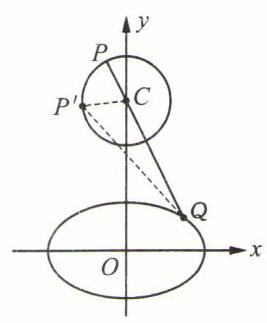
\includegraphics[width=0.2\textwidth]{bodyxb/src/bo_d20cdrf7aajc73bfmvhg_62_1283_1682_267_323_0.jpg}
\end{center}


(第 101 题)

(2)方法一:椭圆上任意一点 $A\left( {x,y}\right)$ 到点 $P$ 的距离为 $\left| {AP}\right|  = \sqrt{{x}^{2} + {\left( y - 1\right) }^{2}}$ ,代入 ${x}^{2} =$  $2\left( {1 - {y}^{2}}\right)$ ,整理得 $\left| {AP}\right|  = \sqrt{2\left( {1 - {y}^{2}}\right)  + {\left( y - 1\right) }^{2}} = \sqrt{-{\left( y + 1\right) }^{2} + 4}$ ,当 $y =  - 1$ 时,即 $A\left( {0, - 1}\right)$ 时,有 ${\left| AP\right| }_{\max } = 2$ . 方法二: (参数方程) 椭圆上任意一点 $A\left( {\sqrt{2}\cos \theta ,\sin \theta }\right) (\theta  \in$  $\lbrack 0,{2\pi }))$ 到点 $P$ 的距离为 $\left| {AP}\right|  = \sqrt{2{\cos }^{2}\theta  + {\left( \sin \theta  - 1\right) }^{2}} = \sqrt{-{\left( \sin \theta  + 1\right) }^{2} + 4}$ ,

$\therefore$ 当 $\theta  = \dfrac{3\pi }{2}$ 时,即 $A\left( {0, - 1}\right)$ 时,有 ${\left| AP\right| }_{\max } = 2$ .

(3)记圆的圆心为 $C\left( {0,4}\right)$ ,不难看出圆 $C$ 与椭圆没有公共点,且圆 $C$ 在椭圆外部. 我们先证明:当 $\left| {PQ}\right|$ 取得最大值时, 点 $P$ 必在射线 ${QC}$ 上. 如图:点 ${P}^{\prime }$ 是圆上与点 $P$ 相异的任意一点,在 $\bigtriangleup {P}^{\prime }{CQ}$ 中 (或点 ${P}^{\prime }$ 是线段 ${QC}$ 与圆 $C$ 的公共点时), $\left| {{P}^{\prime }Q}\right|  \leq  \left| {QC}\right|  + \left| {{P}^{\prime }C}\right|  = \left| {QC}\right|  + \left| {PC}\right|  = \left| {PQ}\right|$ ,证毕. 此时 ${\left| PQ\right| }_{\max } = {r}_{C} + {\left| CQ\right| }_{\max } = 1 + {\left| CQ\right| }_{\max }$ . 设 $Q\left( x\right.$ , $y)$ ,则 $\left| {CQ}\right|  = \sqrt{{x}^{2} + {\left( y - 4\right) }^{2}}$ ,代入 ${x}^{2} = 4\left( {1 - {y}^{2}}\right)$ ,整理得 $\left| {CQ}\right|  = \sqrt{-3{\left( y + \dfrac{4}{3}\right) }^{2} + \dfrac{76}{3}}.\;\because  - 1 \leq  y \leq  1$ , $\therefore$ 当 $y =  - 1$ ,有 ${\left| CQ\right| }_{\max } = 5$ ,故 $\left| {PQ}\right|$ 的最大值是 6,此时 $P\left( {0,5}\right) ,Q\left( {0, - 1}\right)$ .

102. ( 1 )由题意,将 $y = 1 - x$ 代入椭圆方程 ${x}^{2} + b{y}^{2} = \dfrac{3}{4}\left( {b > 0,b \neq  1}\right)$ ,整理得 $\left( {b + 1}\right) {x}^{2} - {2bx} + b - \dfrac{3}{4} = 0,\Delta  =  - b + 3 > 0$ , $\therefore 0 < b < 3$ 且 $b \neq  1$ .

(2)设 $A\left( {{x}_{1},{y}_{1}}\right) ,B\left( {{x}_{2},{y}_{2}}\right)$ ( $\because {AB}$ 中点与原点的连线斜率存在且不为 0, $\therefore {x}_{1} \neq   \pm  {x}_{2}$ ), $M\left( {{x}_{M},{y}_{M}}\right)$ ,则有 ${x}_{1}^{2}$  $+ b{y}_{1}^{2} = {3a},{x}_{2}^{2} + b{y}_{2}^{2} = {3a}$ ,两式相减,并除以 $\left( {{x}_{1} + {x}_{2}}\right) \left( {{x}_{1} - {x}_{2}}\right)$ ,得 $1 + b\dfrac{{y}_{1} + {y}_{2}}{{x}_{1} + {x}_{2}} \cdot  \dfrac{{y}_{1} - {y}_{2}}{{x}_{1} - {x}_{2}} = 0$ ,其中 $\dfrac{{y}_{1} + {y}_{2}}{{x}_{1} + {x}_{2}} =$  $\dfrac{2{y}_{M}}{2{x}_{M}} = \dfrac{{y}_{M} - 0}{{x}_{M} - 0} = \dfrac{1}{5},\dfrac{{y}_{1} - {y}_{2}}{{x}_{1} - {x}_{2}} = {k}_{AB} =  - 1,\therefore b = 5$ . 此时,将 $y = 1 - x$ 代入椭圆方程 ${x}^{2} + 5{y}^{2} = {3a}$ ,整理得 $6{x}^{2} -$  ${10x} + 5 - {3a} = 0,\Delta  = {72a} - {20},\left| {AB}\right|  = \sqrt{1 + {k}_{AB}^{2}} \cdot  \dfrac{\sqrt{\Delta }}{6} = \sqrt{2}\dfrac{\sqrt{{72a} - {20}}}{6} = 2\sqrt{2},\therefore a = \dfrac{41}{18},\therefore$ 椭圆的方程为 ${x}^{2} + 5{y}^{2} = \dfrac{41}{6}.$ 103. 记直线 ${AB}$ 和 ${OM}$ 的斜率分别为 ${k}_{1},{k}_{2}$ . 另设 $A\left( {{x}_{1},{y}_{1}}\right) ,B\left( {{x}_{2},{y}_{2}}\right) (\because {AB}$ 中点与原点的连线斜率存在且不为 0,

$\therefore {x}_{1} \neq   \pm  {x}_{2}$ ), $M\left( {{x}_{M},{y}_{M}}\right)$ . 又, ${b}^{2}{x}_{1}^{2} + {a}^{2}{y}_{1}^{2} = {a}^{2}{b}^{2},{b}^{2}{x}_{2}^{2} + {a}^{2}{y}_{2}^{2} = {a}^{2}{b}^{2}$ ,两式相减,并除以 $\left( {{x}_{1} + {x}_{2}}\right) \left( {{x}_{1} - {x}_{2}}\right)$ ,

得 ${b}^{2} + {a}^{2}\dfrac{{y}_{1} + {y}_{2}}{{x}_{1} + {x}_{2}} \cdot  \dfrac{{y}_{1} - {y}_{2}}{{x}_{1} - {x}_{2}} = 0$ ,其中 $\dfrac{{y}_{1} + {y}_{2}}{{x}_{1} + {x}_{2}} = \dfrac{2{y}_{M}}{2{x}_{M}} = \dfrac{{y}_{M} - 0}{{x}_{M} - 0} = {k}_{2},\dfrac{{y}_{1} - {y}_{2}}{{x}_{1} - {x}_{2}} = {k}_{AB} = 1,\;\therefore \;{b}^{2} =  - {k}_{2} \cdot  {a}^{2}$ .

(1) 由题意, $\left| \dfrac{{k}_{1} - {k}_{2}}{1 + {k}_{1}{k}_{2}}\right|  = 2$ ,其中 ${k}_{1} = 1,\therefore {k}_{2} =  - \dfrac{1}{3}$ 或 ${k}_{2} =  - 3$ . 又 $\because {b}^{2} =  - {k}_{2} \cdot  {a}^{2}$ 且 $a > b > 0$ ,

$\therefore {k}_{2} =  - 3$ (舍去), $\therefore {a}^{2} = 3{b}^{2},c = \sqrt{{a}^{2} - {b}^{2}} = \sqrt{2}b$ . 由题意, $\dfrac{{a}^{2}}{c} = \dfrac{3{b}^{2}}{\sqrt{2}b} = 1$ ,

$\therefore b = \dfrac{\sqrt{2}}{3},\;\therefore \;$ 椭圆方程为 $\dfrac{3{x}^{2}}{2} + \dfrac{9{y}^{2}}{2} = 1$ .

(2) 证法一: 由 $\tan \alpha  = \left| \dfrac{{k}_{1} - {k}_{2}}{1 + {k}_{1}{k}_{2}}\right|  = \left| \dfrac{1 - {k}_{2}}{1 + {k}_{2}}\right|  = \left| \dfrac{1 + \dfrac{{b}^{2}}{{a}^{2}}}{1 - \dfrac{{b}^{2}}{{a}^{2}}}\right|  = \left| \dfrac{{a}^{2} + {b}^{2}}{{a}^{2} - {b}^{2}}\right|  = \left| \dfrac{2{a}^{2} - {c}^{2}}{{c}^{2}}\right|  = \left| \dfrac{2 - c}{c}\right|$ ,可求得 $\dfrac{1}{2} < c < \dfrac{2}{3}(c =$

$\sqrt{{a}^{2} - {b}^{2}}$ ), $\therefore b = \sqrt{c - {c}^{2}} = \sqrt{-{\left( c - \dfrac{1}{2}\right) }^{2} + \dfrac{1}{4}} > \sqrt{-{\left( \dfrac{2}{3} - \dfrac{1}{2}\right) }^{2} + \dfrac{1}{4}} = \dfrac{\sqrt{2}}{3}$ . 又 $b < \dfrac{1}{2}$ . $\therefore \dfrac{\sqrt{2}}{3} < b < \dfrac{1}{2}$ .

证法二: 由题意, $2 < \left| \dfrac{{k}_{1} - {k}_{2}}{1 + {k}_{1}{k}_{2}}\right|  < 3$ ,其中 ${k}_{1} = 1,\therefore {k}_{2} \in  \left( {-3, - 2}\right)  \cup  \left( {-\dfrac{1}{2}, - \dfrac{1}{3}}\right)$ . 又 $\because {b}^{2} =  - {k}_{2} \cdot  {a}^{2}$ 且 $a$

$> b > 0,\;\therefore \; - {k}_{2} < 1,\;\therefore \;{k}_{2} \in  \left( {-\dfrac{1}{2}, - \dfrac{1}{3}}\right)$ . 记 $K =  - \dfrac{1}{{k}_{2}}$ ,则 $K \in  \left( {2,3}\right) ,{a}^{2} = K \cdot  {b}^{2},c = \sqrt{{a}^{2} - {b}^{2}} =$

$\sqrt{K - 1} \cdot  b$ ,直线 $x = \dfrac{{a}^{2}}{c} = \dfrac{K}{\sqrt{K - 1}} \cdot  b = 1,\therefore b = \dfrac{\sqrt{K - 1}}{K} = \sqrt{-{\left( \dfrac{1}{K} - \dfrac{1}{2}\right) }^{2} + \dfrac{1}{4}}$ ,在 $K \in  \left( {2,3}\right)$ 上单调递减, 故 $\dfrac{\sqrt{2}}{3} < b < \dfrac{1}{2}$ ,证毕.

104. (1) 设 $A\left( {{x}_{1},{y}_{1}}\right) ,B\left( {{x}_{2},{y}_{2}}\right) \left( {\because {AB}}\right.$ 不垂直于坐标轴, $\therefore {x}_{1} \neq   \pm  {x}_{2}),P\left( {{x}_{P},{y}_{P}}\right)$ . 又 ${b}^{2}{x}_{1}^{2} + {a}^{2}{y}_{1}^{2} = {a}^{2}{b}^{2},{b}^{2}{x}_{2}^{2} +$  ${a}^{2}{y}_{2}^{2} = {a}^{2}{b}^{2}$ ,两式相减,并除以 $\left( {{x}_{1} + {x}_{2}}\right) \left( {{x}_{1} - {x}_{2}}\right)$ ,得 ${b}^{2} + {a}^{2}\dfrac{{y}_{1} + {y}_{2}}{{x}_{1} + {x}_{2}} \cdot  \dfrac{{y}_{1} - {y}_{2}}{{x}_{1} - {x}_{2}} = 0$ ,其中 $\dfrac{{y}_{1} + {y}_{2}}{{x}_{1} + {x}_{2}} = \dfrac{2{y}_{P}}{2{x}_{P}} = \dfrac{{y}_{P} - 0}{{x}_{P} - 0}$  $= {k}_{OP},\dfrac{{y}_{1} - {y}_{2}}{{x}_{1} - {x}_{2}} = {k}_{AB},\therefore {k}_{AB} \cdot  {k}_{OP} =  - \dfrac{{b}^{2}}{{a}^{2}}$ ,证毕. 注:直线 ${AB}$ 需不垂直于坐标轴,否则 ${k}_{AB},{k}_{OP}$ 必有一个不存在;此外,不论椭圆的焦点在 $x$ 轴上还是 $y$ 轴上,均不影响证明过程,即结论均成立,

(2)若 $b > a > 0$ ,则短轴在 $x$ 轴上,此时 $P$ , $Q$ 就是短轴的两个顶点,因此截距之积为 $- a \cdot  a =  - {a}^{2}$ . 若 $a > b > 0$ ,则短轴在 $y$ 轴上, $B\left( {0,b}\right) ,{B}^{\prime }\left( {0, - b}\right)$ ,令 $M\left( {{x}_{0},{y}_{0}}\right) \left( {{x}_{0} \neq  0}\right)$ ,则 ${l}_{MB} : y = b = \dfrac{{y}_{0} - b}{{x}_{0}} \cdot  x,{l}_{M{B}^{\prime }} : y + b = \dfrac{{y}_{0} + b}{{x}_{0}} \cdot  x$ ,令 $y = 0$ ,

可求得 ${x}_{Q} = \dfrac{-b{x}_{0}}{{y}_{0} - b},{x}_{P} = \dfrac{b{x}_{0}}{{y}_{0} + b}$ ,

$\therefore {x}_{P} \cdot  {x}_{Q} =  - \dfrac{{b}^{2}{x}_{0}^{2}}{{y}_{0}^{2} - {b}^{2}} =  - \dfrac{{a}^{2}\left( {{b}^{2} - {y}_{0}^{2}}\right) }{{y}_{0}^{2} - {b}^{2}} = {a}^{2}$ ,为定值,证毕.

3) $l : {x}_{1}x + 2{y}_{1}y = 2,d = \dfrac{2}{\sqrt{{x}_{1}^{2} + 4{y}_{1}^{2}}} = \dfrac{2}{\sqrt{4 - {x}_{1}^{2}}}$ ,又 ${r}_{1} = a + e{x}_{1} = \sqrt{2} + \dfrac{\sqrt{2}}{2}{x}_{1},{r}_{2} = a - e{x}_{1} = \sqrt{2} - \dfrac{\sqrt{2}}{2}{x}_{1},\;\therefore \;\sqrt{{r}_{1}{r}_{2}}$  $d = \sqrt{2}$ (常数). 注:直线 $l$ 其实是椭圆在点 $A$ 处的切线. 更一般的结论是:对于椭圆 $\dfrac{{x}^{2}}{{a}^{2}} + \dfrac{{y}^{2}}{{b}^{2}} = 1$ (不妨设 $a > b > 0$ ), 过其上一点 $A\left( {{x}_{1},{y}_{1}}\right)$ 作椭圆的切线 $l$ ,沿用本题 ${r}_{1},{r}_{2},d$ 的含义,则此时 $\sqrt{{r}_{1} \cdot  {r}_{2}} \cdot  d$ 为常数 ${ab}$ .

(4) 设 $P\left( {{x}_{0},{y}_{0}}\right)$ ,则由 $\dfrac{{y}_{0}}{{x}_{0}} \cdot  \dfrac{{y}_{0}}{{x}_{0} - a} =  - 1$ 及 $\dfrac{{x}_{0}^{2}}{{a}^{2}} + \dfrac{{y}_{0}^{2}}{{b}^{2}} = 1$ ,消去 ${y}_{0}$ ,得 ${x}_{0} = \dfrac{a{b}^{2}}{{a}^{2} - {b}^{2}}$ ,又 $0 < {x}_{0} < a$ ,由此便得离心率 $e$ 的取值范围是 $\dfrac{\sqrt{2}}{2} < e < 1$ .

105. (1) 对于 $m = c\left( {P\text{ 为右顶点 }}\right) ,\angle {F}_{1}P{F}_{2} = \arccos 1 = 0$ 仍成立. 证法一: $\because {\left| P{F}_{1}\right| }^{2} + {\left| P{F}_{2}\right| }^{2} + 2\left| {P{F}_{1}}\right|  \cdot  \left| {P{F}_{2}}\right|  =$  $4{a}^{2},{\left| P{F}_{1}\right| }^{2} + {\left| P{F}_{2}\right| }^{2} - 2\left| {P{F}_{1}}\right|  \cdot  \left| {P{F}_{2}}\right|  = 4{m}^{2}$ ,两式相减,得 $\left| {P{F}_{1}}\right|  \cdot  \left| {P{F}_{2}}\right|  = {a}^{2} - {m}^{2}.\;\therefore \;\cos \angle {F}_{1}P{F}_{2} =$  $\dfrac{{\left| P{F}_{1}\right| }^{2} + {\left| P{F}_{2}\right| }^{2} - 4{c}^{2}}{2\left| {P{F}_{1}}\right|  \cdot  \left| {P{F}_{2}}\right| } = \dfrac{4{a}^{2} - 2\left( {{a}^{2} - {m}^{2}}\right)  - 4{c}^{2}}{2\left( {{a}^{2} - {m}^{2}}\right) } = \dfrac{{m}^{2} + 2{b}^{2} - {a}^{2}}{{a}^{2} - {m}^{2}}$ . 证法二:由椭圆性质, $\left| {P{F}_{1}}\right|  + \left| {P{F}_{2}}\right|  = {2a}$ ,又已知 $\left| {P{F}_{1}}\right|  - \left| {P{F}_{2}}\right|  = {2m},\therefore \left| {P{F}_{1}}\right|  = a + m,\left| {P{F}_{2}}\right|  = a - m$ ,在 $\bigtriangleup {F}_{1}P{F}_{2}\left( {0 < m < c}\right)$ 中运用余弦定理,即得 $\angle {F}_{1}P{F}_{2} = \arccos \dfrac{{m}^{2} + 2{b}^{2} - {a}^{2}}{{a}^{2} - {m}^{2}}$ . 证毕.

(2)证法一: $\because \dfrac{\left| P{F}_{1}\right| }{\sin \beta } = \dfrac{\left| P{F}_{2}\right| }{\sin \alpha } = \dfrac{2c}{\sin \left( {\alpha  + \beta }\right) },\therefore \dfrac{2a}{\sin \alpha  + \sin \beta } = \dfrac{2c}{\sin \left( {\alpha  + \beta }\right) }$ ,于是 $\dfrac{\cos \dfrac{\alpha  + \beta }{2}}{\cos \dfrac{\alpha  - \beta }{2}} = e$ ,利用合分比性质, 并化积. 得 $\dfrac{\sin \dfrac{\alpha }{2}\sin \dfrac{\beta }{2}}{\cos \dfrac{\alpha }{2}\cos \dfrac{\beta }{2}} = \dfrac{1 - e}{1 + e}$ ,即 $\tan \dfrac{\alpha }{2} \cdot  \tan \dfrac{\beta }{2} = \dfrac{1 - e}{1 + e}$ . 证法二: 证法一是从等式右侧的离心率 $e$ 出发的,我们也可以从等式左侧出发,即通过 $\tan \dfrac{\theta }{2} = \dfrac{1 - \cos \theta }{\sin \theta } = \dfrac{\sin \theta }{1 + \cos \theta }$ 进行证明. 记 $\left| {P{F}_{1}}\right|  = p,\left| {P{F}_{2}}\right|  = q$ . 在 $\bigtriangleup {F}_{1}P{F}_{2}$ 中,由正弦定理,有 $\dfrac{\sin \alpha }{\sin \beta } = \dfrac{q}{p}$ ; 由余弦定理,有 $\dfrac{1}{2}\left( {{q}^{2} + 4{c}^{2} - {p}^{2}}\right)  = {2qc}\cos \beta$ 和 $\dfrac{1}{2}\left( {{p}^{2} + 4{c}^{2} - {q}^{2}}\right)  = {2pc}\cos \alpha$ . $\tan \dfrac{\alpha }{2} \cdot  \tan \dfrac{\beta }{2} = \dfrac{\sin \alpha }{1 + \cos \alpha } \cdot  \dfrac{1 - \cos \beta }{\sin \beta } = \dfrac{{q}^{\prime }}{p} \cdot  \dfrac{1 - \cos \beta }{1 + \cos \alpha } = \dfrac{2qc}{2pc} \cdot  \dfrac{1 - \cos \beta }{1 + \cos \alpha } = \dfrac{{2qc} - \dfrac{1}{2}\left( {{q}^{2} + 4{c}^{2} - {p}^{2}}\right) }{{2pc} + \dfrac{1}{2}\left( {{p}^{2} + 4{c}^{2} - {q}^{2}}\right) } =$  $- \dfrac{{q}^{2} - {4qc} + 4{c}^{2} - {p}^{2}}{{p}^{2} + {4pc} + 4{c}^{2} - {q}^{2}} =  - \dfrac{{\left( q - 2c\right) }^{2} - {p}^{2}}{{\left( p + 2c\right) }^{2} - {q}^{2}}$ . 注意到 $p + q = {2a},\;\therefore \;\tan \dfrac{\alpha }{2} \cdot  \tan \dfrac{\beta }{2} =  - \dfrac{\left( {{2a} - {2c}}\right) \left( {q - p - {2c}}\right) }{\left( {{2a} + {2c}}\right) \left( {p - q + {2c}}\right) } =$  $\dfrac{a - c}{a + c} = \dfrac{1 - e}{1 + e}$ ,证毕.

106. (1) 由题意, $c = 2\sqrt{2},a = \dfrac{c}{e} = 3,\therefore b = 1$ . 又椭圆焦点在 $y$ 轴上, $\therefore$ 椭圆方程为 ${x}^{2} + \dfrac{{y}^{2}}{9} = 1$ .

(2) 设 $M\left( {{x}_{1},{y}_{1}}\right) ,N\left( {{x}_{2},{y}_{2}}\right)$ ( ${MN}$ 的斜率 $k$ 必存在,故 ${x}_{1} \neq  {x}_{2}$ ), ${MN}$ 的中点为 $P\left( {{x}_{P},{y}_{P}}\right)$ ,则有 $\left\{  \begin{array}{l} 9{x}_{1}^{2} + {y}_{1}^{2} = 9, \\  9{x}_{2}^{2} + {y}_{2}^{2} = 9, \end{array}\right.$ 两式相减,并除以 ${x}_{1} - {x}_{2}$ ,得 $9\left( {{x}_{1} + {x}_{2}}\right)  + \left( {{y}_{1} + {y}_{2}}\right) \dfrac{{y}_{1} - {y}_{2}}{{x}_{1} - {x}_{2}} = 0$ . 注意到: ${x}_{1} + {x}_{2} =  - \dfrac{1}{2} \times  2 =  - 1,{y}_{1} + {y}_{2} = 2{y}_{P},k =$  $\dfrac{{y}_{1} - {y}_{2}}{{x}_{1} - {x}_{2}}$ , $\therefore k = \dfrac{9}{2{y}_{P}}$ . 点 $P$ 在直线 $x =  - \dfrac{1}{2}$ 被椭圆截得的线段 (不包含两端点) 上, $\therefore  - \dfrac{3\sqrt{3}}{2} < {y}_{P} < \dfrac{3\sqrt{3}}{2}$ 且 ${y}_{P} \neq  0,\;\therefore \;\left| k\right|  > \sqrt{3},\;\therefore \;l$ 的倾斜角 $\theta$ 的范围是 $\dfrac{\pi }{3} < \theta  < \dfrac{2\pi }{3}$ 且 $\theta  \neq  \dfrac{\pi }{2}$ .

107. (1) 运用第 97(3) 题中我们曾证明过的结论,可知 $A,B,C$ 三点的横坐标也成等差数列,因此 ${x}_{1} + {x}_{3} = 8$ .

(2)设线段 ${AC}$ 的中点为 $M\left( {{x}_{M},{y}_{M}}\right)$ . 将 $A,C$ 两点的坐标代入椭圆方程,运用点差法,易得

$9\left( {{x}_{1} + {x}_{3}}\right) \left( {{x}_{1} - {x}_{3}}\right)  + {25}\left( {{y}_{1} + {y}_{3}}\right) \left( {{y}_{1} - {y}_{3}}\right)  = 0$ . 另外, ${x}_{1} + {x}_{3} = 8 = 2{x}_{M},{y}_{1} + {y}_{3} = 2{y}_{M}$ ,

$\therefore {36}\left( {{x}_{1} - {x}_{3}}\right)  + {25}{y}_{M}\left( {{y}_{1} - {y}_{0}}\right)  = 0$ . 又 ${y}_{1} \neq  {y}_{0}$ . 否则 $A,C$ 或为同一点,或 ${x}_{1} + {x}_{3} = 0$ ,均与题意不符. 线段 ${AB}$

的垂直平分线 $l$ 过点 $M$ ,且斜率为 $k =  - \dfrac{{x}_{1} - {x}_{3}}{{y}_{1} - {y}_{3}} = \dfrac{{25}{y}_{M}}{36},\;\therefore \;l : y - {y}_{M} = k\left( {x - 4}\right)$ ,即 $y = k\left( {x - \dfrac{64}{25}}\right)$ ,过定点 $\left( {\dfrac{64}{25},0}\right)$ ,证毕.

108. (1) 方法一:直线 ${AC},{BD}$ 的方程分别为 $y = x\tan \theta$ 和 $y =  - x\tan \theta$ ,代入椭圆方程,不难求得 $A\left( {-{x}_{0}, - {y}_{0}}\right)$ , $C\left( {x}_{0}\right.$ , $\left. {y}_{0}\right) ,D\left( {-{x}_{0},{y}_{0}}\right) ,B\left( {{x}_{0}, - {y}_{0}}\right)$ ,其中 ${x}_{0} = \dfrac{ab}{\sqrt{{b}^{2} + {a}^{2}{\tan }^{2}\theta }},{y}_{0} = \dfrac{{ab}\tan \theta }{\sqrt{{b}^{2} + {a}^{2}{\tan }^{2}\theta }}$ ,

$\therefore \left| {AC}\right|  = \left| {BD}\right| ,\therefore$ 四边形 ${ABCD}$ 是矩形, $\therefore S = 2{x}_{0} \cdot  2{y}_{0} = \dfrac{4{a}^{2}{b}^{2}\tan \theta }{{b}^{2} + {a}^{2}{\tan }^{2}\theta }$ . 方法二: 对于椭圆上一点 $P$ ,令 $\rho  = \left| {OP}\right|$ . 射线 ${OP}$ 与 $x$ 轴正向所成的角为 $\theta$ . 则 $P$ 的坐标为 $\left( {\rho \cos \theta ,\rho \sin \theta }\right)$ . 代入椭圆方程得 $\dfrac{{\cos }^{2}\theta }{{a}^{2}} + \dfrac{{\sin }^{2}\theta }{{b}^{2}} =$  $\dfrac{1}{{\rho }^{2}}$ ,分别代入 $\theta ,\pi  - \theta ,\theta  + \pi ,{2\pi } - \theta$ ,可得 $\left| {OC}\right|  = \left| {OD}\right|  = \left| {OA}\right|  = \left| {OB}\right|  = {\rho }_{0}$ ,其中 ${\rho }_{0}^{2} = \dfrac{{a}^{2}{b}^{2}}{{b}^{2}{\cos }^{2}\theta  + {a}^{2}{\sin }^{2}\theta }$ ,

$\therefore \left| {AC}\right|  = \left| {BD}\right| ,\therefore$ 四边形 ${ABCD}$ 是矩形, $\therefore S = 2{\rho }_{0}\cos \theta  \cdot  2{\rho }_{0}\sin \theta  = \dfrac{4{a}^{2}{b}^{2}\tan \theta }{{b}^{2} + {a}^{2}{\tan }^{2}\theta }$ .

(2) 由 $S = \dfrac{4{a}^{2}{b}^{2}}{{a}^{2}\tan \theta  + \dfrac{{b}^{2}}{\tan \theta }} \leq  \dfrac{4{a}^{2}{b}^{2}}{2\sqrt{{a}^{2}\tan \theta  \cdot  \dfrac{{b}^{2}}{\tan \theta }}} = {2ab}$ ,得当 $\tan \theta  = \dfrac{b}{a}$ 时, ${S}_{\text{ 最大值 }} = {2ab}$ .

(3) $\because S = \dfrac{4{a}^{2}{b}^{2}}{{a}^{2}\tan \theta  + \dfrac{{b}^{2}}{\tan \theta }}$ ,当 $a > b$ 时, $\tan \theta  = \dfrac{b}{a} \in  \left( {0,1}\right) ,\therefore {S}_{\text{ 最大值 }} = {2ab}$ ; 当 $a < b$ 时, $f\left( \theta \right)  = {a}^{2}\tan \theta  + \dfrac{{b}^{2}}{\tan \theta }$ 在

$\left( {0,\dfrac{\pi }{4}}\right\rbrack$ 上是严格减函数, $\therefore S\left( \theta \right)$ 在 $\left( {0,\dfrac{\pi }{4}}\right\rbrack$ 上是严格增函数, $\therefore {S}_{\text{ 最大值 }} = \dfrac{4{a}^{2}{b}^{2}}{{a}^{2} + {b}^{2}}$ .

结论: ${S}_{\text{ 最大值 }} = \left\{  \begin{array}{l} {2ab}\left( {a > b > 0,\theta  = \arctan \dfrac{b}{a}}\right) , \\  \dfrac{4{a}^{2}{b}^{2}}{{a}^{2} + {b}^{2}}\left( {b > a > 0,\theta  = \dfrac{\pi }{4}}\right) . \end{array}\right.$

109. D 提示: 将方程改写为 $\dfrac{{x}^{2}}{\dfrac{b}{a}} - \dfrac{{y}^{2}}{\dfrac{b}{a}} = 1$ ,由题意, $\dfrac{b}{a} < 0$ ,可以看出,方程表示的是焦点在 $y$ 轴上的双曲线.

110. B 提示: 将方程改写为 $\dfrac{{y}^{2}}{-\dfrac{2}{k}} - \dfrac{{x}^{2}}{-\dfrac{4}{k}} = 1,{a}^{2} =  - \dfrac{2}{k},{b}^{2} =  - \dfrac{4}{k},{c}^{2} = {a}^{2} + {b}^{2} =  - \dfrac{6}{k}$ . 又, ${a}^{2} = c$ ,可解得 $k =  - \dfrac{2}{3}$ .

111. D 提示: 以已知双曲线的虚轴为实轴,实轴为虚轴的双曲线,叫做原双曲线的共轭双曲线. 例如,已知双曲线为 $\dfrac{{x}^{2}}{{a}^{2}} - \dfrac{{y}^{2}}{{b}^{2}}$  $= 1$ ,其顶点为 $\left( {\pm a,0}\right)$ ,焦点为 $\left( {\pm c,0}\right)$ ,渐近线为 $\dfrac{{x}^{2}}{{a}^{2}} - \dfrac{{y}^{2}}{{b}^{2}} = 0$ ,即 $y =  \pm  \dfrac{b}{a}x$ ; 则共轭双曲线为 $\dfrac{{y}^{2}}{{b}^{2}} - \dfrac{{x}^{2}}{{a}^{2}} = 1$ ,其顶点为 $\left( {0, \pm  b}\right)$ ,焦点为 $\left( {0, \pm  c}\right)$ ,渐近线为 $\dfrac{{y}^{2}}{{b}^{2}} - \dfrac{{x}^{2}}{{a}^{2}} = 0$ ,即 $y =  \pm  \dfrac{b}{a}x$ ,可见只有渐近线是相同的.

112. C 提示: 由题意,设双曲线方程为 $\dfrac{{x}^{2}}{{a}^{2}} - \dfrac{{y}^{2}}{{b}^{2}} = 1\left( {a > 0,b > 0}\right)$ ,且 $\left\{  \begin{array}{l} \dfrac{b}{a} = \dfrac{2}{3}, \\  {c}^{2} = {a}^{2} + {b}^{2} = 9, \end{array}\right.$ 解得 $\left\{  \begin{array}{l} {a}^{2} = \dfrac{81}{13}, \\  {b}^{2} = \dfrac{36}{13}, \end{array}\right.$ 因此双曲线方程为 $\dfrac{{13}{x}^{2}}{81} - \dfrac{{13}{y}^{2}}{36} = 1.$

113. A 提示: 设所求双曲线方程为 ${x}^{2} - 2{y}^{2} = \lambda$ ,代入点(2, - 2),可得 $\lambda  =  - 4,\therefore$ 所求双曲线方程为 $- \dfrac{{x}^{2}}{4} + \dfrac{{y}^{2}}{2} = 1$ .

114. B 提示: 由题意, $d = 2 \cdot  \dfrac{{a}^{2}}{c} = c,\;\therefore \;e = \dfrac{c}{a} = \sqrt{2}$ .

115. A 提示: 不难看出,曲线 $\dfrac{{x}^{2}}{{17} - k} + \dfrac{{y}^{2}}{8 - k} = 1$ 表示的是焦点在 $x$ 轴上的双曲线, ${c}^{2} = \left( {{17} - k}\right)  + \left( {k - 8}\right)  = 9,\therefore$ 焦距 ${2c} = 6$ ; 而 $\dfrac{{x}^{2}}{8} + \dfrac{{y}^{2}}{17} = 1$ 表示的是焦点在 $y$ 轴上的椭圆, ${c}^{2} = {17} - 8 = 9,\therefore$ 焦距 ${2c} = 6$ . 因此,两者焦距相同. 此外,由于两条曲线的焦点分别在 $x$ 轴和 $y$ 轴上,因此焦点必不相同; 椭圆没有渐近线; 所有双曲线的离心率都大于 1,而所有椭圆的离心率都小于 1 , 可知离心率必不相同.

116. C 提示: 山题意, $E\left( {-a,0}\right) ,M\left( {0,b}\right) ,F\left( {c,0}\right) ,\therefore \vv{ME} = \left( {-a, - b}\right) ,\vv{MF} = \left( {c, - b}\right) ,\vv{ME} \cdot  \vv{MF} =  - {ac} + {b}^{2} - {c}^{2} -$

${a}^{2} - {ac} = {a}^{2}\left( {{e}^{2} - 1 - e}\right)$ ,代入 $e = \dfrac{\sqrt{5} + 1}{2}$ ,可得 $\vv{ME} \cdot  \vv{MF} = 0$ , $\therefore \angle {EMF} = {90}^{ \circ  }$ (也可由余弦定理得到相同结果).

117. (1) $- \dfrac{{x}^{2}}{20} + \dfrac{{y}^{2}}{5} = 1$ 或 $\dfrac{{x}^{2}}{20} - \dfrac{{y}^{2}}{5} = 1$ 提示: 由题意,设双曲线方程为 $\dfrac{{x}^{2}}{4} - {y}^{2} = \lambda$ . 当焦点在 $x$ 轴上时, $\lambda  > 0$ ,此时有 ${4\lambda } + \lambda$  $= {c}^{2} = {25},\therefore \lambda  = 5,\therefore$ 双曲线方程为 $\dfrac{{x}^{2}}{20} - \dfrac{{y}^{2}}{5} = 1$ ; 当焦点在 $y$ 轴上时, $\lambda  < 0$ ,此时有 $- \lambda  - {4\lambda } = {c}^{2} = {25}$ ,

$\therefore \lambda  =  - 5,\;\therefore$ 双曲线方程为 $- \dfrac{{x}^{2}}{20} + \dfrac{{y}^{2}}{5} = 1$ .

(2) $\dfrac{{x}^{2}}{36} - \dfrac{{y}^{2}}{12} = 1$ 提示:对于椭圆,有 ${a}^{2} = {64},{b}^{2} = {16},\therefore {c}^{2} = {a}^{2} - {b}^{2} = {48}$ ,焦点为 $\left( {\pm c,0}\right)$ . 设所求双曲线方程为 $\dfrac{{x}^{2}}{3}$  $- {y}^{2} = \lambda \left( {\lambda  > 0}\right)$ ,则 ${c}^{2} = {3\lambda } + \lambda  = {48},\therefore \lambda  = {12},\therefore$ 所求双曲线方程为 $\dfrac{{x}^{2}}{36} - \dfrac{{y}^{2}}{12} = 1$ .

(3) $- \dfrac{{x}^{2}}{8} + \dfrac{9{y}^{2}}{32} = 1$ 提示: 设所求双曲线方程为 $4{x}^{2} - 9{y}^{2} = \lambda \left( {\lambda  \neq  0}\right)$ ,代入点(1,2),可得 $\lambda  =  - {32},\therefore$ 所求双曲线方程为 $- \dfrac{{x}^{2}}{8} + \dfrac{9{y}^{2}}{32} = 1$ .

118. (1) ${k\pi } + \dfrac{\pi }{2} < \theta  < {k\pi } + \pi \left( {k \in  \mathbf{Z}}\right)$ 提示:由题意,解不等式: $\sin \theta  \cdot  \cos \theta  < 0 \Leftrightarrow  \sin {2\theta } < 0$ ,其解集为 ${k\pi } + \dfrac{\pi }{2} < \theta  < {k\pi } + \pi \left( {k \in  \mathbf{Z}}\right)$ . (2) $- 2 < m < 2$ 或 $m > 5$ 提示:由题意, $\left( {\left| m\right|  - 2}\right) \left( {5 - m}\right)  < 0$ ,等价于 $\left\{  \begin{array}{l} \left| m\right|  - 2 < 0, \\  5 - m > 0 \end{array}\right.$ 或 $\left\{  \begin{array}{l} \left| m\right|  - 2 > 0, \\  5 - m < 0 \end{array}\right.$ (或者根据 $m \geq  0$ 和 $m < 0$ 解两个二次不等式),解得 $- 2 < m < 2$ 或 $m > 5$ .

(3) $b < m < a\left( {\pm \sqrt{a - b},0}\right)$ 提示:由题意,解不等式 $\left( {a - m}\right) \left( {b - m}\right)  < 0$ ,又 $a > b > 0,\therefore m$ 的取值范围为 $b < m$  $< a$ . 此时曲线方程可改写为 $\dfrac{{x}^{2}}{a - m} - \dfrac{{y}^{2}}{m - b} = 1$ ,是焦点在 $x$ 轴上的双曲线,且 ${c}^{2} = \left( {a - m}\right)  + \left( {m - b}\right)  = a - b$ ,

$\therefore$ 焦点坐标是 $\left( {\pm \sqrt{a - b},0}\right)$ .

(4) $k = 0$ 或 $k =  \pm  3\;k <  - 3$ 或 $k > 3 - 3 < k < 3$ 且 $k \neq  0$ 提示:若曲线 $C$ 表示直线,则 ${x}^{2} \cdot  {y}^{2}$ 的二次项不能同时存在, 故 ${k}^{2}\left( {{k}^{2} - 9}\right)  = 0$ ,解得 $k = 0$ 或 $k =  \pm  3$ ,均满足要求. 当 ${k}^{2}\left( {{k}^{2} - 9}\right)  \neq  0$ 时,曲线 $C$ 可写为 $\dfrac{{x}^{2}}{{k}^{2} - 9} + \dfrac{{y}^{2}}{{k}^{2}} = 1$ . 若曲线 $C$ 表示椭圆,则 $\left\{  \begin{array}{l} {k}^{2} - 9 > 0, \\  {k}^{2} > 0, \\  {k}^{2} - 9 \neq  {k}^{2}, \end{array}\right.$ 解得 $k <  - 3$ 或 $k > 3$ . 若曲线 $C$ 表示双曲线,则 ${k}^{2}\left( {{k}^{2} - 9}\right)  < 0$ ,解得 $- 3 < k < 3$ 且 $k \neq  0$ .

119. (1) arctan $2\sqrt{2}$ 提示:由题意, $a = 2,b = 2\sqrt{2}$ ,渐近线为: $y =  \pm  \dfrac{b}{a}x =  \pm  \sqrt{2}x$ ,记两条渐近线的斜率为 ${k}_{1} = \sqrt{2},{k}_{2} =$  $- \sqrt{2}$ ,则两渐近线的夹角 $\theta$ 的正切为 $\tan \theta  = \left| \dfrac{{k}_{1} - {k}_{2}}{1 + {k}_{1}{k}_{2}}\right|  = 2\sqrt{2},\therefore \theta  = \arctan 2\sqrt{2}$ .

(2) $\dfrac{2\sqrt{3}}{3}$ 提示:设原双曲线的实半轴长 $a = k$ ,则半焦距长 $c = {ea} = {2k}$ ,虚半轴长 $b = \sqrt{{c}^{2} - {a}^{2}} = \sqrt{3}k$ ；根据共轭双曲线的定义,其实半轴长是原双曲线的虚半轴长,虚半轴长是原双曲线的实半轴长,故半焦距不变, $\therefore$ 共轭双曲线的离心率 ${e}^{\prime } = \dfrac{2k}{\sqrt{3}k} = \dfrac{2\sqrt{3}}{3}$ .

(3) $- \dfrac{3}{32}$ 提示:双曲线的焦点在 $x$ 轴上,故将双曲线改写为 $\dfrac{{x}^{2}}{-\dfrac{1}{k}} - \dfrac{{y}^{2}}{-\dfrac{1}{2k}} = 1,\;\therefore \;{c}^{2} =  - \dfrac{1}{k} - \dfrac{1}{2k} = {\left( -4\right) }^{2}$ ,

$\therefore k =  - \dfrac{3}{32}$ .

(4) $\dfrac{5}{4}$ 或 $\dfrac{5}{3}$ 提示: 双曲线方程可以写为 $9{x}^{2} - {16}{y}^{2} = \lambda$ . 当 $\lambda  > 0$ 时,双曲线焦点在 $x$ 轴上,此时 ${a}^{2} = \dfrac{\lambda }{9},{b}^{2} = \dfrac{\lambda }{16},{c}^{2} =$  ${a}^{2} + {b}^{2} = \dfrac{25\lambda }{144},\;\therefore \;e = \dfrac{c}{a} = \sqrt{\dfrac{25}{16}} = \dfrac{5}{4}$ ; 当 $\lambda  < 0$ 时,双曲线焦点在 $y$ 轴上,此时 ${a}^{2} =  - \dfrac{\lambda }{16},{b}^{2} =  - \dfrac{\lambda }{9},{c}^{2} = {a}^{2} + {b}^{2}$  $=  - \dfrac{25\lambda }{144},\;\therefore \;e = \dfrac{c}{a} = \sqrt{\dfrac{25}{9}} = \dfrac{5}{3}.$

120. A 提示: 由题意,解不等式 $\left( {2 - m}\right) \left( {\left| m\right|  - 3}\right)  < 0$ ,等价于 $\left\{  \begin{array}{l} 2 - m > 0, \\  \left| m\right|  - 3 < 0 \end{array}\right.$ 或 $\left\{  \begin{array}{l} 2 - m < 0, \\  \left| m\right|  - 3 > 0 \end{array}\right.$ (或者根据 $m \geq  0$ 和 $m < 0$ 解两个二次不等式). 解得 $- 3 < m < 2$ 或 $m > 3$ .

121. D 提示: 由题意,设双曲线方程为 ${25}{y}^{2} - {144}{x}^{2} = \lambda \left( {\lambda  > 0}\right)$ . 此时, ${a}^{2} = \dfrac{\lambda }{25},{b}^{2} = \dfrac{\lambda }{144},{c}^{2} = {a}^{2} + {b}^{2} = \dfrac{169}{{25} \times  {144}}\lambda$ ,

$\therefore \dfrac{{a}^{2}}{c} = \dfrac{\dfrac{\lambda }{25}}{\dfrac{13}{5 \times  {12}}\sqrt{\lambda }} = \dfrac{144}{13}$ ,解得 $\lambda  = {3600}.\;\therefore$ 双曲线方程为 $- \dfrac{{x}^{2}}{25} + \dfrac{{y}^{2}}{144} = 1$ .

122. B 提示: 由题意, $a = 8$ ,点 $P$ 到左焦点的距离为 ${14} + {16} = {30}$ .

123. D 提示: 由题意,双曲线的渐近线为 $y =  \pm  \dfrac{5}{4}x$ ,记 ${k}_{1} = \dfrac{5}{4},{k}_{2} =  - \dfrac{5}{4}$ ,则两条渐近线的夹角 $\theta$ 的正切是 $\left| \dfrac{{k}_{1} - {k}_{2}}{1 + {k}_{1}{k}_{2}}\right|  =$  $\dfrac{40}{9}$ ,故 $\theta  = \arctan \dfrac{40}{9}$ . 注:选项 (C) $2\arctan \dfrac{5}{4}$ 是错误的,因为它是一个钝角 ( $\arctan \dfrac{5}{4} > \arctan 1 = \dfrac{\pi }{4}$ ),而 $\pi  - 2\arctan \dfrac{5}{4}$ 则是正确的,且可以证明 $\pi  - 2\arctan \dfrac{5}{4} = \arctan \dfrac{40}{9}$ .

124. (1) 由题意, $2\lg {2y} = \lg \left( {x - 2}\right)  + \lg {16x},\therefore 4{y}^{2} = {16x}\left( {x - 2}\right) \left( {x > 2,y > 0}\right)$ ,整理得 ${\left( x - 1\right) }^{2} - \dfrac{{y}^{2}}{4} = 1\left( {x > 2,y > 0}\right)$ ,是中心在(1,0),原点在 $x$ 轴上的双曲线的一部分.

(2)由题意,椭圆的右焦点为 $\left( {\sqrt{{169} - {144}},0}\right)$ ,即(5,0),记为点 $C$ ；双曲线的渐近线是 $y =  \pm  \dfrac{4}{3}x$ . 点 $C$ 到双曲线的两条渐近线的距离均为 $\dfrac{\left| \dfrac{4}{3} \times  5\right| }{\sqrt{1 + {\left( \pm \dfrac{4}{3}\right) }^{2}}} = 4$ ,即圆 $C$ 的半径, $\therefore$ 圆 $C$ 的方程为 ${\left( x - 5\right) }^{2} + {y}^{2} = {16}$ .

(3)双曲线的焦点为 $\left( {\pm \sqrt{\dfrac{1}{4} + \dfrac{3}{4}},0}\right)$ ,即(±1,0). 设椭圆方程为 $\dfrac{{x}^{2}}{{a}^{2}} + \dfrac{{y}^{2}}{{a}^{2} - 1} = 1\left( {a > 1}\right)$ ,代入直线 $y = x + 3$ ,整理得 $\left( {2{a}^{2} - 1}\right) {x}^{2} + 6{a}^{2}x + {a}^{2}\left( {{10} - {a}^{2}}\right)  = 0,\Delta  = 8{a}^{2}\left( {{a}^{2} - 1}\right) \left( {{a}^{2} - 5}\right)  \geq  0,\;\therefore \;{a}^{2} \geq  5$ ,长轴最短时, ${a}^{2} = 5,\;\therefore$ 椭圆方程为 $\dfrac{{x}^{2}}{5} + \dfrac{{y}^{2}}{4} = 1$ .

125. (1) 双曲线的左焦点是 $F\left( {-\sqrt{\dfrac{3}{4} + \dfrac{1}{4}},0}\right)$ ,即 $F\left( {-1,0}\right)$ . 所求直线的斜率存在,设为 $k$ ,由题意: $\left| \dfrac{k - 2}{1 + {2k}}\right|  = \tan \dfrac{\pi }{4} =$ 1,解得 $k =  - 3$ 或 $k = \dfrac{1}{3}$ ,故所求直线方程为 ${3x} + y + 3 = 0$ 或 $x - {3y} + 1 = 0$ .

(2)将 $y = {3x} + 3$ 代入双曲线方程,整理得 $5{x}^{2} + {18x} + {13} = 0$ ,

故所求线段长为 $\sqrt{1 + {k}^{2}}\dfrac{\sqrt{\Delta }}{5} = \sqrt{1 + {3}^{2}}\dfrac{\sqrt{{18}^{2} - 4 \times  5 \times  {13}}}{5} = \dfrac{8}{5}\sqrt{10}$ .

(3) $a = 3,b = 4,c = 5$ ,双曲线的右焦点为(5,0). 直线 ${AB}$ 的方程为 $y = x - 5$ ,代入双曲线,整理得 $7{x}^{2} + {90x} - {369} = 0$ , 故所求弦长为 $\left| {AB}\right|  = \sqrt{1 + {k}^{2}}\dfrac{\sqrt{\Delta }}{7} = \sqrt{1 + {1}^{2}}\dfrac{\sqrt{{90}^{2} + 4 \times  7 \times  {369}}}{7} = \dfrac{192}{7}$ ; 又 ${x}_{M} = \dfrac{{x}_{1} + {x}_{2}}{2} =  - \dfrac{45}{7}$ ,

$\therefore {y}_{M} = {x}_{M} - 5 =  - \dfrac{80}{7},\therefore \left| {MF}\right|  = \sqrt{{\left( -\dfrac{45}{7} - 5\right) }^{2} + {\left( -\dfrac{80}{7}\right) }^{2}} = \dfrac{80}{7}\sqrt{2}$ . 注: 在学习过圆锥曲线的统一极坐标方程后,可以有更快的解法:双曲线对应的极坐标方程为: $\rho  = \dfrac{ep}{1 - e\cos \theta }$ ,不妨设 $A,B$ 两点的极坐标为 $A\left( {{\rho }_{1},\dfrac{\pi }{4}}\right)$ , $B\left( {{\rho }_{2},\dfrac{5\pi }{4}}\right)$ ,不难看出 ${\rho }_{1} < 0 < {\rho }_{2}$ ,即 $A,B$ 两点分别在双曲线的两支上,

$\therefore \left| {AB}\right|  = \left| {{\rho }_{1} + {\rho }_{2}}\right|  = \left| {\dfrac{ep}{1 - e\cos \dfrac{\pi }{4}} + \dfrac{ep}{1 - e\cos \dfrac{5\pi }{4}}}\right|  = \dfrac{2ep}{\left| 1 - \dfrac{1}{2}{e}^{2}\right| },\left| {MF}\right|  = {\rho }_{2} + \dfrac{1}{2}\left| {AB}\right|  = \dfrac{{\rho }_{2} - {\rho }_{1}}{2} = \dfrac{\sqrt{2}{e}^{2}p}{{e}^{2} - 2}$ .

其中 $e = \dfrac{c}{a} = \dfrac{5}{3},p = \dfrac{{b}^{2}}{c} = \dfrac{16}{5},\;\therefore \;\left| {AB}\right|  = \dfrac{192}{7},\left| {MF}\right|  = \dfrac{80}{7}\sqrt{2}$ .

126. $C$ 提示: 不妨设双曲线方程为 $\dfrac{{x}^{2}}{{a}^{2}} - \dfrac{{y}^{2}}{{b}^{2}} = 1,{F}_{1}\left( {-c,0}\right) ,{F}_{2}\left( {c,0}\right)$ . 由双曲线关于坐标轴的对称性可知: $\operatorname{Rt}\bigtriangleup {F}_{1}{F}_{2}P$ 中, $\angle P{F}_{1}{F}_{2} = \dfrac{\pi }{4},\angle {F}_{1}{F}_{2}P = \dfrac{\pi }{2},\therefore \left| {{F}_{2}P}\right|  = \left| {{F}_{2}{F}_{1}}\right|  = {2c}$ ,即双曲线过点 $\left( {c,{2c}}\right) ,\therefore \dfrac{{c}^{2}}{{a}^{2}} - \dfrac{4{c}^{2}}{{b}^{2}} = 1$ ,注意到 $\dfrac{{c}^{2}}{{a}^{2}} - 1$  $= \dfrac{{b}^{2}}{{a}^{2}}$ , $\therefore {2ac} = {b}^{2} = {c}^{2} - {a}^{2}$ . 再代入 $c = {ea}$ ,可得方程 ${e}^{2} - {2e} - 1 = 0,e > 1$ , $\therefore e = \sqrt{2} + 1$ .

127. D 提示:将直线方程代入双曲线,整理得 $\left( {1 - {k}^{2}}\right) {x}^{2} - {4kx} - {10} = 0$ ,由题意,该方程有两个不同的正实根,故列出不等式

组 $\left\{  \begin{array}{l} 1 - {k}^{2} \neq  0, \\  \Delta  = {16}{k}^{2} + {40}\left( {1 - {k}^{2}}\right)  > 0, \\  {x}_{1} + {x}_{2} = \dfrac{4k}{1 - {k}^{2}} > 0,\;\text{ 解得 }k \in  \left( {-\dfrac{\sqrt{15}}{3}, - 1}\right) . \\  {x}_{1}{x}_{2} = \dfrac{-{10}}{1 - {k}^{2}} > 0, \end{array}\right.$

128. B 提示:方法一:将直线方程代入双曲线,整理得 $- \dfrac{1}{9}\left( {-{7x} + \dfrac{49}{4}}\right)  = 1$ ,解得 $x = \dfrac{85}{28}$ ,对应地, $y =  - \dfrac{13}{84}$ ,因此本题中,直线与双曲线只有一个公共点. 方法二: 双曲线的焦点在 $x$ 轴上,右支与 $x$ 轴的交点为(3,0),渐近线为 $y =  \pm  \dfrac{1}{3}x$ . 直线 $y$  $= \dfrac{1}{3}\left( {x - \dfrac{7}{2}}\right)$ 过点 $\left( {\dfrac{7}{2},0}\right)$ (在点 $A$ 右侧),且与双曲线的一条渐近线 $y = \dfrac{1}{3}x$ 平行,因此直线与双曲线右支在第四象限有一个公共点, 而与双曲线左支无公共点.

129. D 提示: 由题意, $\tan \theta  = \dfrac{b}{a}$ . 将 $x = c$ (或 $x =  - c$ ) 代入双曲线方程,得 $y =  \pm  \dfrac{{b}^{2}}{a}$ ,故所求弦长为 $\dfrac{2{b}^{2}}{a} = {2b} \cdot  \tan \theta$ .

130. C 提示: 方法一: 由题意,轨迹上的任意一点(x, y)满足: $\dfrac{\sqrt{{\left( x - 5\right) }^{2} + {y}^{2}}}{\left| x - \dfrac{16}{5}\right| } = \dfrac{5}{4}$ ,整理得 $\dfrac{{x}^{2}}{16} - \dfrac{{y}^{2}}{9} = 1$ .

* 方法二:由于定直线垂直于 $x$ 轴,定点在 $x$ 轴上, $\dfrac{5}{4} > 1$ , $\therefore$ 动点的轨迹是焦点在 $x$ 轴上的双曲线；又,定点到定

直线的距离为 $\dfrac{9}{5},\therefore \left\{  {\begin{array}{l} e = \dfrac{c}{a} = \dfrac{5}{4}, \\  c = \dfrac{{a}^{2}}{c} = \dfrac{{b}^{2}}{c} = \dfrac{9}{5}, \\  {c}^{2} = {a}^{2} + {b}^{2}, \end{array}\text{ 解得 }\left\{  \begin{array}{l} a = 4, \\  b = 3,\text{ 又根据定直线在定点左侧,可知定点 }A\text{ 恰为双曲线的右焦点, } \\  c = 5, \end{array}\right. }\right.$

$\therefore$ 双曲线方程为 $\dfrac{{x}^{2}}{16} - \dfrac{{y}^{2}}{9} = 1$ . 注: 根据定点 $A\left( {5,0}\right)$ ,直接得出 $c = 5$ ,或根据定直线 $l : x = \dfrac{16}{5}$ ,直接得出 $\dfrac{{a}^{2}}{c} = \dfrac{16}{5}$ ,都是用错误的方法得到正确的结果, 因为题干没有说明双曲线的中心在原点.

131. C 提示: 记圆 ${x}^{2} + {y}^{2} = 1$ 的圆心为 $A\left( {0,0}\right)$ ,半径为 1 ; 圆 ${x}^{2} + {y}^{2} - {8x} + 7 = 0$ 的圆心为 $B\left( {4,0}\right)$ ,半径为 3,两圆外切于点 $D\left( {1,0}\right)$ . 设动圆的圆心为 $P\left( {x,y}\right)$ . 圆 $P$ 与圆 $A$ 或圆 $B$ 的相切有三类: 外切、内切 (圆 $P$ 包含圆 $A$ 或圆 $B$ )、内切 (圆 $A$ 或圆 $B$ 包含圆 $P)$ ,共计 $3 \times  3 = 9$ (种)情况,如下表:

\begin{center}
\adjustbox{width=\textwidth}{
\begin{tabular}{|c|c|c|c|c|}
\hline
\multicolumn{2}{|c|}{\phantom{X}} & 与圆 $B$ 外切 & \multicolumn{2}{|c|}{与圆 $B$ 内切} \\
\cline{3-5}
\multicolumn{2}{|c|}{\phantom{X}} & $\left| {PB}\right|  = r + 3$ & $\left| {PB}\right|  = r - 3$ & $\left| {PB}\right|  = 3 - r$ \\
\cline{1-5}
与圆 $A$ 外切 & $\left| {PA}\right|  = r + 1$ & $\left| {PA}\right|  - \left| {PB}\right|  =  - 2$ & $\left| {PA}\right|  - \left| {PB}\right|  = 4$ & $\left| {PA}\right|  + \left| {PB}\right|  = 4$ \\
\cline{1-5}
\multirow{2}{*}{与圆 $A$ 内切} & $\left| {PA}\right|  = r - 1$ & $\left| {PA}\right|  - \left| {PB}\right|  =  - 4$ & $\left| {PA}\right|  - \left| {PB}\right|  = 2$ & $\left| {PA}\right|  + \left| {PB}\right|  = 2$ \\
\cline{2-5}
 & $\left| {PA}\right|  = 1 - r$ & $\left| {PA}\right|  + \left| {PB}\right|  = 4$ & $\left| {PA}\right|  + \left| {PB}\right|  =  - 2$ & $\left| {PA}\right|  - \left| {PB}\right|  =  - 2$ \\
\cline{1-5}
\hline
\end{tabular}
}
\end{center}

9 种情况最后归结为关于 $\left| {PA}\right|$ 和 $\left| {PB}\right|$ 的 3 种可能关系: $\text{ ① }\left| \right| {PA}\left| -\right| {PB}\left| \right|  = 2$ ,点 $P$ 的轨迹 ${C}_{1}$ 是双曲线,其中心在 ( 2 , $0),{2a} = 2,{2c} = \left| {AB}\right|  = 4,\therefore {C}_{1} : {\left( x - 2\right) }^{2} - \dfrac{{y}^{2}}{3} = 1;$ ② $\left| \right| {PA}\left| \pm \right| {PB}\left| \right|  = 4$ ,但这并不代表椭圆或双曲线,根据三角不等式,事实上此时点 $P$ 在直线 ${AB}$ 上,点 $P$ 的轨迹 ${C}_{2} : y = 0$ ; ③ $\left| {PA}\right|  + \left| {PB}\right|  = 2$ ,根据三角不等式, $\left| {PA}\right|  + \left| {PB}\right|  \geq$  $\left| {AB}\right|  = 4$ ,因此不存在这样的点 $P$ . 因此圆心 $P$ 的轨迹是一条双曲线和一条直线,但要去掉 $A,B,D$ 三点,具体情况见下表:

\begin{center}
\adjustbox{width=\textwidth}{
\begin{tabular}{|c|c|c|c|c|}
\hline
\multicolumn{2}{|c|}{\phantom{X}} & 与圆 $B$ 外切 & \multicolumn{2}{|c|}{与圆 $B$ 内切} \\
\cline{3-5}
\multicolumn{2}{|c|}{\phantom{X}} & $\left| {PB}\right|  = r + 3$ & $\left| {PB}\right|  = r - 3$ & $\left| {PB}\right|  = 3 - r$ \\
\cline{1-5}
与圆 $A$ 外切 & $\left| {PA}\right|  = r + 1$ & ${C}_{1}$ 左支 去掉点 $D\left( {1,0}\right)$ & ${C}_{2}\left( {x > 4}\right)$ & ${C}_{2}\left( {1 < x < 4}\right)$ \\
\cline{1-5}
\multirow{2}{*}{与圆 $A$ 内切} & $\left| {PA}\right|  = r - 1$ & ${C}_{2}\left( {x < 0}\right)$ & ${C}_{1}$ 右支 & 不存在 \\
\cline{2-5}
 & $\left| {PA}\right|  = 1 - r$ & ${C}_{2}\left( {0 < x < 1}\right)$ & 不存在 & 不存在 \\
\cline{1-5}
\hline
\end{tabular}
}
\end{center}

132. $B$ 提示:由题意, $F\left( {-\sqrt{2},0}\right)$ . 方法一:双曲线在第三象限的表达式是 $y =  - \sqrt{{x}^{2} - 1}$  $\left( {x <  - 1}\right) ,\therefore k = \dfrac{y - 0}{x + \sqrt{2}} = \dfrac{-\sqrt{{x}^{2} - 1}}{x + \sqrt{2}}$ . 当 $- \sqrt{2} < x <  - 1$ 时, $k$ 是单调递增的,此时 $k \in  \left( {-\infty ,0}\right)$ ; 当 $x <  - \sqrt{2}$ 时, $k = \dfrac{\sqrt{{x}^{2} - 1}}{-\left( {x + \sqrt{2}}\right) }$ . 令 $t =  - \left( {x + \sqrt{2}}\right)$ ,则 $k = \dfrac{\sqrt{{\left( -t - \sqrt{2}\right) }^{2} - 1}}{t} = \sqrt{{\left( \dfrac{1}{t} + \sqrt{2}\right) }^{2} - 1}\left( {t > 0}\right)$ ,不难看出此时 $k$ 在 $t > 0$ 上单调递减,故 $k \in  \left( {1, + \infty }\right)$ . 综上, $k < 0$ 或 $k > 1$ . 方法二: (结合图形) 如图,不难直接看出最终的结论,下面给出证明: 记 ${y}_{1} = k\left( {x + \sqrt{2}}\right) ,{y}_{2} =  - \sqrt{{x}^{2} - 1}\left( {x <  - 1}\right) ,g\left( x\right)  = {y}_{1} -$  ${y}_{2}$ ,将 $k$ 分几种情况讨论: ① $k < 0$ ,此时 $g\left( x\right)$ 在区间 $\left\lbrack  {-\sqrt{2}, - 1}\right\rbrack$ 上单调递减,且 $g\left( {-\sqrt{2}}\right)  > 0 > g\left( {-1}\right)$ ,因此,对任意的 $k < 0$ ,总能找到一个点 $P$ ,且其横坐标在区间 $\left( {-\sqrt{2}, - 1}\right)$ 上,使得 ${PF}$ 的斜率为 $k;\text{ ② }k = 0$ ,显然,直线与双曲线在第三象限没有公共点； $\text{ ③ }k > 1$ ,此时 ${y}_{1} = k\left( {x + \sqrt{2}}\right)$ 与渐近线 $y = x$ 有交点 $P\left( {{x}_{P},{y}_{P}}\right)$ , 其中 ${x}_{P} = \dfrac{\sqrt{2}k}{1 - k} <  - \sqrt{2}$ ,根据渐近线的性质, $g\left( {x}_{P}\right)  < 0$ ,又 $g\left( {-\sqrt{2}}\right)  = 1 > 0$ ,故对任意的 $k > 1$ ,总能找到一点 $P$ ,且其横坐标在区间 $\left( {{x}_{P}, - \sqrt{2}}\right)$ 上,使得 ${PF}$ 的斜率为 $k;{40} < k \leq  1$ ,记渐近线 ${y}_{3} = x$ ,则 $g\left( x\right)  = {y}_{1} - {y}_{3} + {y}_{3} - {y}_{2}$ ,在区间 $( - \infty , - 1\rbrack$ 上, ${y}_{1} - {y}_{3}$ 单调递减 (或为定值),根据渐近线的性质, ${y}_{3} - {y}_{2}$ 严格单调递减, $\therefore g\left( x\right)$ 在区间 $( - \infty$ , 一1]上单调递减, $\therefore g\left( x\right)  \geq  g\left( {-1}\right)  > 0$ ,因此 $g\left( x\right)  = 0$ 在区间 $( - \infty , - 1\rbrack$ 上无解,即此时直线与双曲线在第三象限没有公共点. 综上, $k < 0$ 或 $k > 1$ . 注: 方法一相当于遍历了双曲线在第三象限的每一点,得到了 $k$ 的取值范围,同时得到了 $k$ 的单调性. 方法二相当于遍历了 $k$ 在 $\mathbf{R}$ 上的所有可能,但这一方法只能告诉我们对于特定的 $k$ ,能不能找到这样的点 $P$ 与之对应 (存在性). 因此即使我们知道了 $k < 0$ 或 $k > 1$ 满足条件,也必须说明 $0 \leq  k \leq  1$ 时找不到这样的点 $P$ . 另外,方法二也不能保证点 $P$ 的唯一性,以及讨论 $k$ 变化的趋势.

\begin{center}
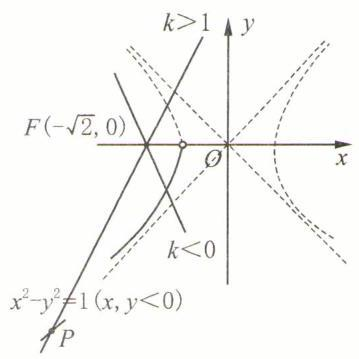
\includegraphics[width=0.3\textwidth]{bodyxb/src/bo_d20cdrf7aajc73bfmvhg_69_1080_128_359_359_0.jpg}
\end{center}


(第 132 题)

133. D 提示: $y = \sqrt{\left| 1 - {x}^{2}\right| }$ 的定义域是 $\mathbf{R}$ ,据此可知选项 $\vv{a},\vv{b},\mathbf{C}$ 均错误; 根据 ${x}^{2}$ 的不同取值,原方程可整理为 ${x}^{2} + {y}^{2} = 1$  $\left( {y \geq  0\text{ ,半圆 }}\right)$ 和 ${x}^{2} - {y}^{2} = 1\left( {y \geq  0\text{ ,双曲线的上半部 }}\right)$ ,因此 D 符合题意.

134. $C$ 提示: 由题意,方程 ${mx} - y + n = 0$ 代表斜率为 $m$ ,在 $y$ 轴上的截距为 $n$ 的直线; 方程 $n{x}^{2} + m{y}^{2} = {mn}$ 代表二次曲线 $\dfrac{{x}^{2}}{m} + \dfrac{{y}^{2}}{n} = 1$ ,如下表可知,只有选项 $C$ 正确.

\begin{center}
\adjustbox{width=\textwidth}{
\begin{tabular}{|c|c|c|}
\hline
\phantom{X} & 直线 & 二次曲线 \\
\cline{1-3}
(A) & $m > 0,n < 0$ & $m > n > 0$ \\
\cline{1-3}
(B) & $m < 0,n > 0$ & $n > m > 0$ \\
\cline{1-3}
(C) & $m > 0,n < 0$ & $m > 0 > n$ \\
\cline{1-3}
(D) & $m > 0,n > 0$ & $n > 0 > m$ \\
\cline{1-3}
\hline
\end{tabular}
}
\end{center}

注: 选项 (C) 暗示直线和双曲线在第四象限有一个公共点,这还要求 $- n > {m}^{\dfrac{3}{2}}$ ,读者可以自行验证这一点.

135. A 提示: 由椭圆和双曲线的性质: ${\left( \left| P{F}_{1}\right|  + \left| P{F}_{2}\right| \right) }^{2} = {\left( 2\sqrt{m}\right) }^{2},{\left( \left| P{F}_{1}\right|  - \left| P{F}_{2}\right| \right) }^{2} = {\left( 2\sqrt{a}\right) }^{2}$ ,两式相减并除以 4,可得 $\left| {P{F}_{1}}\right|  \cdot  \left| {P{F}_{2}}\right|  = m - a$ .

136. A 提示: 曲线 ${\left( x - 1\right) }^{2} + {y}^{2} = 1$ 代表圆心 $C\left( {1,0}\right)$ ,半径为 1 的圆,且完全处于 $x \geq  0$ 的区域. 当 $a = 0$ 时, ${x}^{2} - {y}^{2} = {a}^{2} = 0$ 表示两条直线 $y =  \pm  x$ ,与圆 $C$ 有三个公共点:(0,0)和 $\left( {1, \pm  1}\right)$ . 当 $a \neq  0$ 时, ${x}^{2} - {y}^{2} = {a}^{2}$ 表示焦点在 $x$ 轴上的双曲线, 它与圆 $C$ 的公共点只可能处在双曲线的右支,且如果存在一个公共点(x, y),那(x, - y)也一定是一个公共点. 现已知公共点有奇数个,则必有公共点的纵坐标是 0,代入圆 $C$ 和双曲线方程,得 $\left\{  {\begin{array}{l} {x}^{2} = {a}^{2}, \\  {\left( x - 1\right) }^{2} = 1, \end{array}a \neq  0,\therefore a =  \pm  2}\right.$ ,此时圆 $C$ 和双曲线只有 1 个公共点(2,0),不合题意. 综上 $a = 0$ 是唯一解. 注:当 $a \neq  0$ 时,也可将圆 $C$ 和双曲线方程联立,消去 ${y}^{2}$ ,得到 $2{x}^{2} - {2x} - {a}^{2} = 0$ ,其 $\Delta  > 0$ ,两根之和为正( 1 ),两根之积为负 $\left( {-\dfrac{{a}^{2}}{2}}\right)$ ,可见只有一个正根,故圆 $C$ 和双曲线最多只有 2 个公共点, 不合题意.

137. (1) 证法一: 可设这条渐近线为 $y = \dfrac{b}{a}x$ ,于是得 $P\left( {\dfrac{{a}^{2}}{c},\dfrac{ab}{c}}\right)$ ,再证 ${k}_{PF} \cdot  {k}_{OP} =  - 1$ . 证法二: 一般结论对直线 $x =  \pm  \dfrac{{a}^{2}}{c}$ 和 $F\left( {\pm c,0}\right)$ 都成立. 由于渐近线均过原点 $O$ ,只需证明 $\vv{FP} \cdot  \vv{OP} = 0$ . 记点 $P$ 的坐标 $P\left( {{x}_{P},{y}_{P}}\right) ,F\left( {\pm c,0}\right)$ ,则 $\vv{FP} =$  $\left( {{x}_{P} \mp  c,{y}_{P}}\right) ,\vv{OP} = \left( {{x}_{P},{y}_{P}}\right) ,\;\therefore \vv{FP} \cdot  \vv{OP} = {x}_{P}^{2} \mp  c{x}_{P} + {y}_{P}^{2}$ ,其中 $\mp  c{x}_{P} = \left( {\mp c}\right)  \cdot  \left( {\pm \dfrac{{a}^{2}}{c}}\right)  =  - {a}^{2}$ ,由渐近线方

程可知 ${y}_{P}^{2} = \dfrac{{b}^{2}}{{a}^{2}} \cdot  {x}_{P}^{2},\therefore \vv{FP} \cdot  \vv{OP} = \left( {1 + \dfrac{{b}^{2}}{{a}^{2}}}\right) {x}_{P}^{2} - {a}^{2} = \dfrac{{c}^{2}}{{a}^{2}} \cdot  \dfrac{{a}^{4}}{{c}^{2}} - {a}^{2} = 0$ ,点 $P$ 在四个象限的四种可能均证毕.

(2)方法一: $\left| {PF}\right|  = \left| {OF}\right|  \cdot  \sin \angle {POF} = b$ . 方法二:在(1)中,我们已知 $\vv{FP} \cdot  \vv{OP} = {x}_{P}^{2} - c{x}_{P} + {y}_{P}^{2} = {x}_{P}^{2} + {y}_{P}^{2} - {a}^{2} = 0$ , $\therefore {\left| OP\right| }^{2} = {x}_{P}^{2} + {y}_{P}^{2} = {a}^{2}$ ,又 ${\left| OF\right| }^{2} = {c}^{2}$ ,运用勾股定理得 $\left| {PF}\right|  = \sqrt{{\left| OF\right| }^{2} - {\left| OP\right| }^{2}} = b$ .

138. 方法一: 令 $\angle {F}_{1}P{F}_{2} = \theta ,\left| {P{F}_{1}}\right|  = m,\left| {P{F}_{2}}\right|  = n$ ,则由余弦定理可得 ${mn} = \dfrac{6}{1 - \cos \theta }$ ,又由 ${S}_{\bigtriangleup {F}_{1}P{F}_{2}} = \dfrac{1}{2}m \cdot  n\sin \theta  = 3\sqrt{3}$ , 于是 $\dfrac{\sin \theta }{1 - \cos \theta } = \sqrt{3}$ ,得 $\theta  = \dfrac{\pi }{3}$ . 需注意,余弦定理得到的方程 ${m}^{2} + {n}^{2} - {2mn}\cos \theta  = {\left( 2c\right) }^{2} = {32}$ 中, ${m}^{2} + {n}^{2}$ 可以由 ${\left( m - n\right) }^{2}$  $= {\left( 2a\right) }^{2}$ 的展开式表达为: ${m}^{2} + {n}^{2} = {20} + {2mn}$ ; 另外,解三角方程时,可使用 $\dfrac{\sin \theta }{1 - \cos \theta } = \cot \dfrac{\theta }{2}$ 方便求解. 方法二: 仍然记 $\angle {F}_{1}P{F}_{2} = \theta ,\left| {P{F}_{1}}\right|  = m,\left| {P{F}_{2}}\right|  = n$ . 设点 $P$ 的坐标为 $P\left( {{x}_{P},{y}_{P}}\right) ,\left| {{F}_{1}{F}_{2}}\right|  = {2c} = 2\sqrt{5 + 3} = 4\sqrt{2},\therefore {S}_{\bigtriangleup {F}_{1}P{F}_{2}} =$  $\dfrac{1}{2}\left| {{F}_{1}{F}_{2}}\right|  \cdot  \left| {y}_{P}\right| ,\;\therefore \left| {y}_{P}\right|  = \dfrac{3}{4}\sqrt{6}\left( {{y}_{P}^{2} = \dfrac{27}{8}}\right)$ ,代入双曲线方程,得 ${x}_{P}^{2} = \dfrac{85}{8}$ . 在 $\bigtriangleup {F}_{1}P{F}_{2}$ 中使用余弦定理,得 ${m}^{2} +$  ${n}^{2} - {2mn}\cos \theta  = {\left( 2c\right) }^{2} = {32}$ ,用 ${\left( m - n\right) }^{2} = {\left( 2a\right) }^{2}$ 的展开式消去 ${mn}$ ,得 $\cos \theta  = \dfrac{{32} - \left( {{m}^{2} + {n}^{2}}\right) }{{20} - \left( {{m}^{2} + {n}^{2}}\right) }$ . 而 ${m}^{2} + {n}^{2} = {\left( {x}_{P} + c\right) }^{2} + {y}_{P}^{2}$  $+ {\left( {x}_{P} - c\right) }^{2} + {y}_{P}^{2} = 2\left( {{x}_{P}^{2} + {y}_{P}^{2} + {c}^{2}}\right)  = {44},\;\therefore \;\cos \theta  = \dfrac{1}{2},\theta  = \dfrac{\pi }{3}$ .

*139. 记 $\left| {P{F}_{1}}\right|  = {t}_{1},\left| {P{F}_{2}}\right|  = {t}_{2}$ ,并假设双曲线左半支上存在点 $P$ ,使 ${t}_{1}^{2} = d{t}_{2}$ ,则由 $\dfrac{{t}_{1}}{d} = e$ ,得 ${t}_{2} = e{t}_{1}$ ,结合 ${t}_{2} - {t}_{1} = {2a}$ ,得 ${t}_{1}$  $= \dfrac{2a}{e - 1},{t}_{2} = \dfrac{2ea}{e - 1}$ . 再利用 ${t}_{1} + {t}_{2} \geq  {2c}$ ,求得 $1 < e \leq  1 + \sqrt{2}$ ,这与已知 “ $e > 1 + \sqrt{2}$ ” 相矛盾, $\;\therefore$ 满足条件的点 $P$ 不存在.

140. (1) 椭圆的焦点是 $\left( {0, \pm  \sqrt{5}}\right) ,{PQ}$ 边的中点是原点 $O\left( {0,0}\right)$ . 记重心为 $G\left( {x,y}\right)$ ,则由重心的性质, $\vv{OM} = \vv{3OG}$ ,得 $M({3x}$ , ${3y})$ ,代入双曲线方程,整理得 $\dfrac{9{x}^{2}}{25} - {y}^{2} = 1$ .

(2)若直线斜率不存在,不难看出 $M\left( {2,0}\right)$ ,以下求解直线斜率 $k$ 存在的情况. 方法一:设 $P\left( {{x}_{1},{y}_{1}}\right) ,Q\left( {{x}_{1},{y}_{2}}\right)$ ,直线方程为 $y - 1 = k\left( {x - 2}\right)$ ,代入 $2{x}^{2} - {y}^{2} = 2$ ,整理得 $\left( {2 - {k}^{2}}\right) {x}^{2} + {2k}\left( {{2k} - 1}\right) x - \left( {4{k}^{2} - {4k} + 3}\right)  = 0,{k}^{2} \neq  2$ 时 $\Delta  = 8\left( {3{k}^{2}}\right.$  $- {4k} + 4)$ 恒大于 0,此时 ${x}_{M} = \dfrac{{x}_{1} + {x}_{2}}{2} = \dfrac{k\left( {{2k} - 1}\right) }{{k}^{2} - 2},{y}_{M} = k\left( {{x}_{M} - 2}\right)  + 1 = \dfrac{2\left( {{2k} - 1}\right) }{{k}^{2} - 2}$ . 记 $x = {x}_{M},y = {y}_{M}$ .

$\therefore {ky} = {2x},\;\therefore k\left( {x - 2}\right) y = \left( {y - 1}\right) y = {2x}\left( {x - 2}\right)$ ,整理得 $C : 2{x}^{2} - {y}^{2} - {4x} + y = 0$

方法二: (点差法) 设 $P\left( {{x}_{1},{y}_{1}}\right) ,Q\left( {{x}_{2},{y}_{2}}\right) \left( {{x}_{1} \neq  {x}_{2}}\right) ,M\left( {x,y}\right)$ . 将 $P,Q$ 代入双曲线方程,得 $2{x}_{1}^{2} - {y}_{1}^{2} = 2,2{x}_{2}^{2} - {y}_{2}^{2}$  $= 2$ ,两式相减并除以 $\left( {{x}_{1} - {x}_{2}}\right)$ ,得 $2\left( {{x}_{1} + {x}_{2}}\right)  - \left( {{y}_{1} + {y}_{2}}\right) \dfrac{{y}_{1} - {y}_{2}}{{x}_{1} - {x}_{2}} = 0$ ,代入 ${x}_{1} + {x}_{2} = {2x},{y}_{1} + {y}_{2} = {2y},\dfrac{{y}_{1} - {y}_{2}}{{x}_{1} - {x}_{2}} =$  $\dfrac{y - 1}{x - 2}$ ,整理得 $C : 2{x}^{2} - {y}^{2} - {4x} + y = 0$ ,注意到 $M\left( {2,0}\right)$ 也满足方程. 最后,我们来说明轨迹 $C$ 上的每一点都能被取到. 设轨迹 $C$ 上的任意一点 $\left( {{x}_{0},{y}_{0}}\right)$ ,直线 ${PQ}$ 的方程为 $l : \left( {{y}_{0} - 1}\right) \left( {x - 2}\right)  - \left( {{x}_{0} - 2}\right) \left( {y - 1}\right)  = 0$ ,我们只需证明直线 ${PQ}$ 与原双曲线总有两个不同公共点即可. ①当 ${x}_{0} = 2$ 时, ${y}_{0} = 0\left( {l : x = 2}\right)$ 或 ${y}_{0} = 1$ (点 $A$ 和点 $M$ 重合,由 $2\left( {x}_{1}\right.$  $\left. {+{x}_{2}}\right)  - \left( {{y}_{1} + {y}_{2}}\right) \dfrac{{y}_{1} - {y}_{2}}{{x}_{1} - {x}_{2}} = 0$ ,可求得 $\left. {\dfrac{{y}_{1} - {y}_{2}}{{x}_{1} - {x}_{2}} = 4,l : {4x} - y - 7 = 0}\right)$ ,不难验证与原双曲线有两个不同公共点; ②当 ${x}_{0} = 0$ 时, ${y}_{0} = 0\left( {l : y = \dfrac{1}{2}x}\right)$ 或 ${y}_{0} = 1\left( {l : y = 1}\right)$ ,不难验证与原双曲线有两个不同公共点; ③ 当 ${x}_{0} \neq  0,2$ 时, $l : y - 1$  $= \dfrac{{y}_{0} - 1}{{x}_{0} - 2}\left( {x - 2}\right)  = \dfrac{2{x}_{0}}{{y}_{0}}\left( {x - 2}\right)$ ,令 $t = \dfrac{2{x}_{0}}{{y}_{0}}\left( {{t}^{2} \neq  2}\right.$ ,否则 ${y}_{0} =  \pm  \sqrt{2}{x}_{0}$ ,结合曲线 $C$ 可知, ${y}_{0} = {x}_{0} = 0$ ,与 ${x}_{0} \neq  0,2$ 矛盾),则 $l : y = t\left( {x - 2}\right)  + 1$ 代入 $2{x}^{2} - {y}^{2} = 2$ ,整理得 $\left( {2 - {t}^{2}}\right) {x}^{2} + {2t}\left( {{2t} - 1}\right) x - \left( {4{t}^{2} - {4t} + 3}\right)  = 0$ ,该二次方程的 $\Delta  =$  $8\left( {3{t}^{2} - {4t} + 4}\right)$ 恒大于 0, $\therefore$ 直线 $l$ 与原双曲线有两个不同的公共点. 综上,所求轨迹方程为 $C : 2{x}^{2} - {y}^{2} - {4x} +$  $y = 0$ . 注:判断方程上哪些点是符合要求的,是求解轨迹时必需的步骤.

(3)设 $R$ 是 $\bigtriangleup  {ABC}$ 的外接圆半径,由题意, ${2R}\sin B - {2R}\sin C = \dfrac{1}{2} \cdot  {2R}\sin A$ ,根据正弦定理,有 $\left| {AC}\right|  - \left| {AB}\right|  = \dfrac{1}{2}$ . $\left| {BC}\right|  = 6$ ,可见顶点 $A$ 在焦点为 $\left( {\pm {6.0}}\right)$ 的双曲线 $\dfrac{{x}^{2}}{{a}^{2}} - \dfrac{{y}^{2}}{{b}^{2}} = 1$ 的左支上,其中 $a = \dfrac{6}{2} = 3,b = \sqrt{{6}^{2} - {3}^{2}} = 3\sqrt{3}$ ,

$\therefore$ 顶点 $A$ 的轨迹为 $\dfrac{{x}^{2}}{9} - \dfrac{{y}^{2}}{27} = 1\left( {x < 0\text{ 且 }x \neq   - 3}\right)$ .

(4)两圆的圆心分别为 $A\left( {-5,0}\right) ,B\left( {5,0}\right)$ ,半径分别为 ${r}_{1} = 7,{r}_{2} = 1$ . 设动圆 $P$ 的半径为 $R$ ,由题意, $\left| {PA}\right|  = R + {r}_{1} =$  $R + 7,\left| {PB}\right|  = R + {r}_{2} = R + 1,\therefore \left| {PA}\right|  - \left| {PB}\right|  = 6,\therefore$ 点 $P$ 在焦点为 $\left( {\pm 5,0}\right)$ 的双曲线 $\dfrac{{x}^{2}}{{a}^{2}} - \dfrac{{y}^{2}}{{b}^{2}} = 1$ 的右支

上,其中 $a = \dfrac{6}{2} = 3,b = \sqrt{{5}^{2} - {3}^{2}} = 4,\therefore$ 动点 $P$ 的轨迹方程为 $\dfrac{{x}^{2}}{9} - \dfrac{{y}^{2}}{16} = 1\left( {x > 0}\right)$

(5)设双曲线的另一个焦点是 ${F}^{\prime }$ ,则 $\left| {O{F}^{\prime }}\right|  - \left| {OF}\right| \left| { = {2a} = 4\text{ ，其中 }}\right| {OF} \mid   = 4$ , $\therefore \left| {O{F}^{\prime }}\right|  = 0$ (舍)或 $\left| {O{F}^{\prime }}\right|  = 8$ . 此时 ${F}^{\prime }$ 在圆 ${x}^{2} + {y}^{2} = {64}$ 上,需特别考察 $O,F,{F}^{\prime }$ 三点共线的情况 (即 $y = 0$ ). 当 ${F}^{\prime }\left( {-8,0}\right)$ 时,双曲线存在,为 $\dfrac{{\left( x + 2\right) }^{2}}{4}$  $- \dfrac{{y}^{2}}{32} = 1$ ; 当 ${F}^{\prime }\left( {8,0}\right)$ 时,双曲线不存在. 双曲线中心,即线段 $F{F}^{\prime }$ 的中点,记为 $M\left( {x,y}\right)$ ,且有 $\left\{  \begin{array}{l} {x}_{{F}^{\prime }} = {2x} - 4, \\  {y}_{{F}^{\prime }} = {2y}, \end{array}\right.$ 代入 ${x}^{2} + {y}^{2} = {64}$ ,整理得 ${\left( x - 2\right) }^{2} + {y}^{2} = {16}\left( {x \neq  6}\right)$ .

(6) 设 $P\left( {t,t}\right) \left( {t > 0}\right) ,\because \angle {POQ} = \dfrac{\pi }{2},\therefore {S}_{\bigtriangleup {POQ}} = \dfrac{1}{2}\left| {OP}\right|  \cdot  \left| {OQ}\right|  = \dfrac{\sqrt{2}}{2}t \cdot  \left| {OQ}\right|  = 1$ ,

$\therefore \left| {OQ}\right|  = \dfrac{\sqrt{2}}{t},\;\therefore Q\left( {\dfrac{1}{t}, - \dfrac{1}{t}}\right)$ . 线段 ${PQ}$ 的中点 $M\left( {x,y}\right)$ 满足 $\left\{  \begin{array}{l} x = \dfrac{1}{2}\left( {t + \dfrac{1}{t}}\right) , \\  y = \dfrac{1}{2}\left( {t - \dfrac{1}{t}}\right) , \end{array}\right.$

$\therefore \left\{  \begin{array}{l} x + y = t, \\  x - y = \dfrac{1}{t}, \end{array}\right.$ 消去 $t$ ,得 ${x}^{2} - {y}^{2} = 1\left( {x > 0\text{ 或更严格地, }x \geq  1}\right)$ .

141. (1) 设弦的两端点为 $B\left( {{x}_{1},{y}_{1}}\right) ,C\left( {{x}_{2},{y}_{2}}\right) \left( {{x}_{1} \neq  {x}_{2}}\right.$ ,否则弦的中点的纵坐标为 0 ),代入双曲线方程,得 ${x}_{1}^{2} - 4{y}_{1}^{2} = {16}$ , ${x}_{2}^{2} - 4{y}_{2}^{2} = {16}$ ,两式相减,并除以 $\left( {{x}_{1} - {x}_{2}}\right)$ ,得 $\left( {{x}_{1} + {x}_{2}}\right)  - 4\left( {{y}_{1} + {y}_{2}}\right) \dfrac{{y}_{1} - {y}_{2}}{{x}_{1} - {x}_{2}} = 0$ ,代入 ${x}_{1} + {x}_{2} = 2{x}_{A} = 2,{y}_{1} + {y}_{2} =$  $2{y}_{A} = 2$ ,得 ${k}_{AB} = \dfrac{{y}_{1} - {y}_{2}}{{x}_{1} - {x}_{2}} = \dfrac{1}{4}$ ,故弦所在直线方程为 ${l}_{BC} : y - 1 = \dfrac{1}{4}\left( {x - 1}\right)$ ,即 ${l}_{BC} : x - {4y} + 3 = 0$ (可以验证直线 ${BC}$ 与双曲线有两个不同的公共点).

(2)设 $M\left( {{x}_{1},{y}_{1}}\right) ,N\left( {{x}_{2},{y}_{2}}\right) \left( {{x}_{1} \neq  {x}_{2}}\right.$ ,否则弦的中点的纵坐标为 0 ),代入双曲线方程,得 ${x}_{1}^{2} - 2{y}_{1}^{2} = 8,{x}_{2}^{2} - 2{y}_{2}^{2} = 8$ ,两式相减,并除以 $\left( {{x}_{1} - {x}_{2}}\right)$ ,得 $\left( {{x}_{1} + {x}_{2}}\right)  - 2\left( {{y}_{1} + {y}_{2}}\right) \dfrac{{y}_{1} - {y}_{2}}{{x}_{1} - {x}_{2}} = 0$ ,代入 ${x}_{1} + {x}_{2} = 2{x}_{P} =  - 4,{y}_{1} + {y}_{2} = 2{y}_{P} = 4$ ,得 ${k}_{MN} = \dfrac{{y}_{1} - {y}_{2}}{{x}_{1} - {x}_{2}} =  - \dfrac{1}{2}$ ,故弦所在直线方程为 ${l}_{MN} : y - 2 =  - \dfrac{1}{2}\left( {x + 2}\right)$ ,即 ${l}_{MN} : x + {2y} - 2 = 0$ . 再代入双曲线方程,消去 $y$ ,得 ${x}^{2} + {4x} - {20} = 0$ , $\therefore \;\left| {MN}\right|  = \sqrt{1 + {k}_{MN}^{2}}\dfrac{\sqrt{\Delta }}{1} = \sqrt{1 + \dfrac{1}{4}}\sqrt{{4}^{2} + 4 \times  1 \times  {20}} = 2\sqrt{30}$ .

(3)若存在,设 $C\left( {{x}_{1},{y}_{1}}\right) ,D\left( {{x}_{2},{y}_{2}}\right) \left( {{x}_{1} \neq  {x}_{2}}\right.$ ,否则弦的中点的纵坐标为 0 ),代入双曲线方程,得 $2{x}_{1}^{2} - {y}_{1}^{2} = 2,2{x}_{2}^{2} - {y}_{2}^{2}$  $= 2$ ,两式相减,并除以 $\left( {{x}_{1} - {x}_{2}}\right)$ ,得 $2\left( {{x}_{1} + {x}_{2}}\right)  - \left( {{y}_{1} + {y}_{2}}\right) \dfrac{{y}_{1} - {y}_{2}}{{x}_{1} - {x}_{2}} = 0$ ,代入 ${x}_{1} + {x}_{2} = 2{x}_{N} = 2,{y}_{1} + {y}_{2} = 2{y}_{N} = 2$ , 得 ${k}_{CD} = \dfrac{{y}_{1} - {y}_{2}}{{x}_{1} - {x}_{2}} = 2$ ,故弦所在直线方程为 ${l}_{CD} : y - 1 = 2\left( {x - 1}\right)$ ,即 ${l}_{CD} : {2x} - y - 1 = 0$ . 再代入双曲线方程,消去 $y$ , 得 $2{x}^{2} - {4x} + 3 = 0,\Delta  =  - 8 < 0$ ,可见不存在满足题意的直线.

142. 将直线方程代入双曲线,并消去 $y$ ,整理得 ${x}^{2} - {2bx} - \left( {{b}^{2} + 2}\right)  = 0,\Delta  = 8\left( {{b}^{2} + 1}\right)  > 0$ . 方法一: 设 $A\left( {{x}_{1},{y}_{1}}\right) ,B\left( {{x}_{2},{y}_{2}}\right)$ , 则由条件可得 ${x}_{1} + {x}_{2} = {2b},{x}_{1}{x}_{2} =  - {b}^{2} - 2,{y}_{1}{y}_{2} =  - {x}_{1}{x}_{2}$ ,得 $b =  \pm  2$ . 需注意, ${y}_{1}{y}_{2} =  - {x}_{1}{x}_{2}$ 是利用了直径对应的圆周角为 ${90}^{ \circ  }$ ,故 $\vv{OA} \cdot  \vv{OB} = {x}_{1}{x}_{2} + {y}_{1}{y}_{2} = 0$ . 另外, ${y}_{1}{y}_{2} = \left( {{x}_{1} + b}\right) \left( {{x}_{2} + b}\right)  = {x}_{1}{x}_{2} + b\left( {{x}_{1} + {x}_{2}}\right)  + {b}^{2}$ . 方法二: 以 ${AB}$ 为直径的圆的圆心 $C\left( {{x}_{C},{y}_{C}}\right)$ 满足: ${x}_{C} = \dfrac{{x}_{1} + {x}_{2}}{2} = b,{y}_{C} = {x}_{C} + b = {2b};{2r} = \left| {AB}\right|  = \sqrt{1 + {k}_{AB}^{2}}\dfrac{\sqrt{\Delta }}{1} = \sqrt{2}\sqrt{8\left( {{b}^{2} + 1}\right) } =$  $4\sqrt{{b}^{2} + 1},$

$\therefore$ 圆 $C$ 的方程为 ${\left( x - b\right) }^{2} + {\left( y - 2b\right) }^{2} = 4\left( {{b}^{2} + 1}\right)$ ,代入点(0,0),解得 $b =  \pm  2$ .

143. (1) 设椭圆和双曲线的方程分别为 $\dfrac{{x}^{2}}{{a}_{1}^{2}} + \dfrac{{y}^{2}}{{b}_{1}^{2}} = 1$ 和 $\dfrac{{x}^{2}}{{a}_{2}^{2}} - \dfrac{{y}^{2}}{{b}_{2}^{2}} = 1$ . 由题意得 ${c}_{1} = {c}_{2} = c = \sqrt{13}$ ,又, $\left\{  \begin{array}{l} {a}_{1} - {a}_{2} = 4, \\  \dfrac{{e}_{1}}{{e}_{2}} = \dfrac{\dfrac{{c}_{1}}{{a}_{2}}}{\dfrac{{e}_{2}}{{a}_{2}}} = \dfrac{3}{7}, \end{array}\right.$ 解得 $\left\{  {\begin{array}{l} {a}_{1} = 7, \\  {a}_{2} = 3. \end{array}{b}_{1} = \sqrt{{a}_{1}^{2} - {c}_{1}^{2}} = 6,{b}_{2} = \sqrt{{c}_{2}^{2} - {a}_{2}^{2}} = 2,\;\therefore }\right.$ 椭圆方程为 $\dfrac{{x}^{2}}{49} + \dfrac{{y}^{2}}{36} = 1$ ,双曲线方程为 $\dfrac{{x}^{2}}{9} - \dfrac{{y}^{2}}{4} = 1$ .

(2)不妨假设 $\left| {P{F}_{1}}\right|  > \left| {P{F}_{2}}\right|$ ,则有 $\left\{  {\begin{array}{l} \left| {P{F}_{1}}\right|  + \left| {P{F}_{2}}\right|  = 2{a}_{1} \\  \left| {P{F}_{1}}\right|  - \left| {P{F}_{2}}\right|  = 2{a}_{2}, \end{array}\;\therefore \left\{  {\begin{array}{l} \left| {P{F}_{1}}\right|  = {a}_{1} + {a}_{2}, \\  \left| {P{F}_{2}}\right|  = {a}_{1} - {a}_{2}, \end{array}\text{ 由余弦定理得 }\cos \angle {F}_{1}P{F}_{2} = }\right. }\right.$  $\dfrac{{\left| P{F}_{1}\right| }^{2} + {\left| P{F}_{2}\right| }^{2} - {\left| {F}_{1}{F}_{2}\right| }^{2}}{2\left| {P{F}_{1}}\right| \left| {P{F}_{2}}\right| } = \dfrac{{a}_{1}^{2} + {a}_{2}^{2} - 2{c}^{2}}{{a}_{1}^{2} - {a}_{2}^{2}} = \dfrac{4}{5}.$

144. (1) 不妨假设 $\left| {P{F}_{1}}\right|  > \left| {P{F}_{2}}\right|$ ,由题意得 $\left\{  {\begin{array}{l} \left| {P{F}_{1}}\right|  + \left| {P{F}_{2}}\right|  = {2a}, \\  \left| {P{F}_{1}}\right|  - \left| {P{F}_{2}}\right|  = {2m}, \end{array}\;\therefore \;\left\{  {\begin{array}{l} \left| {P{F}_{1}}\right|  = a + m, \\  \left| {P{F}_{2}}\right|  = a - m, \end{array}\;\therefore \;\left| {P{F}_{1}}\right|  \cdot  \left| {P{F}_{2}}\right|  = {a}^{2}}\right. }\right.$  $- {m}^{2}$ .

(2)方法一:记 $\left| {P{F}_{1}}\right|  = p$ , $\left| {P{F}_{2}}\right|  = q$ ,利用余弦定理,可得 ${2pq}\left( {1 + \cos \alpha }\right)  = 4{b}^{2}$ , ${2pq}\left( {1 - \cos \alpha }\right)  = 4{n}^{2}$ ,相除便得. 注意, 在证明中,还需用到 ${\left( p + q\right) }^{2} = 4{a}^{2}$ 和 ${\left( p - q\right) }^{2} = 4{m}^{2}$ 来消去 ${p}^{2} + {q}^{2}$ . 方法二: 记 $\angle {F}_{1}P{F}_{2} = \alpha$ ,记 $\left| {{F}_{1}{F}_{2}}\right|  = {2c}$ ,则由余弦定理得 $\cos \alpha  = \dfrac{{\left| P{F}_{1}\right| }^{2} + {\left| P{F}_{2}\right| }^{2} - {\left| {F}_{1}{F}_{2}\right| }^{2}}{2\left| {P{F}_{1}}\right| \left| {P{F}_{2}}\right| } = \dfrac{{a}^{2} + {m}^{2} - 2{c}^{2}}{{a}^{2} - {m}^{2}},1 + \cos \alpha  = \dfrac{2{b}^{2}}{{a}^{2} - {m}^{2}},1 - \cos \alpha  = \dfrac{2{n}^{2}}{{a}^{2} - {m}^{2}}$ ,又 $\alpha$  $\in  \left( {0,\pi }\right) ,$

$\therefore \tan \dfrac{\alpha }{2} = \sqrt{\dfrac{1 - \cos \alpha }{1 + \cos \alpha }} = \dfrac{n}{b},\;\therefore \angle {F}_{1}P{F}_{2} = 2\arctan \dfrac{n}{b}$ ,证毕. 注:注: ${a}^{2} - {b}^{2} = {c}^{2} = {m}^{2} + {n}^{2}$ .

(3) 方法一:将上两式相乘,得 ${p}^{2} \cdot  {q}^{2}{\sin }^{2}\alpha  = 4{b}^{2} \cdot  {n}^{2},\;\therefore S = \dfrac{1}{2}{pq}\sin \alpha  = {bn}$ . 方法二:由 (1) (2) 可得 $\sin \alpha  =$  $\dfrac{2\tan \dfrac{\alpha }{2}}{1 + {\tan }^{2}\dfrac{\alpha }{2}} = \dfrac{2\dfrac{n}{b}}{1 + \dfrac{{n}^{2}}{{b}^{2}}} = \dfrac{2nb}{{b}^{2} + {n}^{2}},\;\therefore \;{S}_{\bigtriangleup {F}_{1}P{F}_{2}} = \dfrac{1}{2}\left| {P{F}_{1}}\right| \left| {P{F}_{2}}\right| \sin \alpha  = \left( {{a}^{2} - {m}^{2}}\right) \dfrac{nb}{{b}^{2} + {n}^{2}}$ ,注意到 ${a}^{2} - {b}^{2} = {c}^{2} = {m}^{2}$  $+ {n}^{2},\;\therefore \;{a}^{2} - {m}^{2} = {b}^{2} + {n}^{2},\;\therefore \;{S}_{\bigtriangleup {F}_{1}P{F}_{2}} = {bn}.$

方法三:由(1)(2),我们注意到 $\bigtriangleup {F}_{1}P{F}_{2}$ 的三边长为 $a + m,a - m,{2c}$ ,因此可使用海伦公式: $p = a + c,{S}_{\bigtriangleup {F}_{1}P{F}_{2}} =$  $\sqrt{p\left( {p - \left| {P{F}_{1}}\right| }\right) \left( {p - \left| {P{F}_{2}}\right| }\right) \left( {p - \left| {{F}_{1}{F}_{2}}\right| }\right) } = \sqrt{\left( {a + c}\right) \left( {c - m}\right) \left( {c + m}\right) \left( {a - c}\right) } = {bn}.$

45. 不妨设 ${F}_{1}\left( {c,0}\right)$ 是双曲线的右焦点. 证法一:①若直线 ${AB}$ 的斜率为 0,即 ${l}_{AB} : y = 0$ ,不难看出,以线段 ${AB}$ 为直径的圆的圆心是 $C\left( {0,0}\right)$ ,半径为 $a$ ,即 $\odot  C : {x}^{2} + {y}^{2} = {a}^{2}$ ,圆心到直线 $x = \dfrac{{a}^{2}}{c}$ 的距离是 $d = \dfrac{{a}^{2}}{c} < a$ ,故圆 $C$ 与直线 $x = \dfrac{{a}^{2}}{c}$ 相交, $\overset{⏜}{MN}$ 的度数为 $2\arccos \dfrac{d}{a} = 2\arccos \dfrac{1}{e}$ . ②若直线 ${AB}$ 的斜率不为 0 或斜率不存在,设 ${l}_{AB} : {ky} = x - c$  $\left( {k \neq   \pm  \dfrac{a}{b}}\right.$ ,否则直线与双曲线只有一个公共点),代入双曲线方程 ${b}^{2}{x}^{2} - {a}^{2}{y}^{2} = {a}^{2}{b}^{2}$ ,消去 $x$ ,整理得 $\left( {{b}^{2}{k}^{2} - {a}^{2}}\right) {y}^{2} +$  $2{b}^{2}{cky} + {b}^{4} = 0,\Delta  = 4{b}^{4}{c}^{2}{k}^{2} - 4{b}^{4}\left( {{b}^{2}{k}^{2} - {a}^{2}}\right)  = 4{a}^{2}{b}^{4}\left( {{k}^{2} + 1}\right)  > 0$ ,因此直线 ${AB}$ 和双曲线总是有两个公共点. 设线段

${AB}$ 的中点 $C\left( {{x}_{C},{y}_{C}}\right)$ ,根据韦达定理,有 ${y}_{C} = \dfrac{{b}^{2}{ck}}{{a}^{2} - {b}^{2}{k}^{2}}$ ,从而 ${x}_{C} = k{y}_{C} + c = \dfrac{{a}^{2}c}{{a}^{2} - {b}^{2}{k}^{2}}$ ,以线段 ${AB}$ 为直径的圆 $C$ ,其半

径 ${r}_{C} = \dfrac{1}{2}\left| {AB}\right|  = \dfrac{1}{2}\sqrt{1 + {k}^{2}}\dfrac{\sqrt{\Delta }}{\left| {b}^{2}{k}^{2} - {a}^{2}\right| } = \dfrac{a{b}^{2}\left( {1 + {k}^{2}}\right) }{\left| {b}^{2}{k}^{2} - {a}^{2}\right| }$ . 圆 $C$ 到直线 $x = \dfrac{{a}^{2}}{c}$ 的距离为 $d = \left| {\dfrac{{a}^{2}c}{{a}^{2} - {b}^{2}{k}^{2}} - \dfrac{{a}^{2}}{c}}\right|  = \dfrac{a}{c}$ . $\dfrac{a{b}^{2}\left( {1 + {k}^{2}}\right) }{\left| {b}^{2}{k}^{2} - {a}^{2}\right| } = \dfrac{{r}_{C}}{e}$ ( $e$ 是离心率), $\because e > 1,\therefore d < {r}_{C}$ ,故圆 $C$ 与直线 $x = \dfrac{{a}^{2}}{c}$ 相交, $\overset{⏜}{MN}$ 的度数为 $2\arccos \dfrac{d}{{r}_{C}} = 2\arccos \dfrac{1}{e}$ .

综上, $\overset{⏜}{MN}$ 的度数为定值 $2\arccos \dfrac{1}{e}$ ,证毕. 证法二: 记 $A\left( {{x}_{1},{y}_{1}}\right) ,B\left( {{x}_{2},{y}_{2}}\right)$ ,线段 ${AB}$ 的中点为 $C\left( {{x}_{C},{y}_{C}}\right) ,e$ 是双曲线的离心率. 以线段 ${AB}$ 的中点为圆心的圆 $C$ ,圆心到直线 $x = \dfrac{{a}^{2}}{c}$ 的距离为 $d = \left| {{x}_{C} - \dfrac{{a}^{2}}{c}}\right|  = \left| {\dfrac{{x}_{1} + {x}_{2}}{2} - \dfrac{{a}^{2}}{c}}\right|  =$  $\dfrac{1}{2}\left| {\left( {{x}_{1} - \dfrac{{a}^{2}}{c}}\right)  + \left( {{x}_{2} - \dfrac{{a}^{2}}{c}}\right) }\right|$ . $A,B$ 两点有两种情况: ① 都在双曲线的同一支 (这里是右支),此时 $d =$  $\dfrac{1}{2}\left| {\left( {{x}_{1} - \dfrac{{a}^{2}}{c}}\right)  + \left( {{x}_{2} - \dfrac{{a}^{2}}{c}}\right) }\right|  = \dfrac{1}{2}\left| {\dfrac{\left| CA\right| }{e} + \dfrac{\left| CB\right| }{e}}\right|  = \dfrac{\left| AB\right| }{2} \cdot  \dfrac{1}{e} = \dfrac{{r}_{C}}{e}$ ; ② 分属双曲线的两支,此时 $d =$  $\dfrac{1}{2}\left| {\left( {{x}_{1} - \dfrac{{a}^{2}}{c}}\right)  + \left( {{x}_{2} - \dfrac{{a}^{2}}{c}}\right) }\right|  = \dfrac{1}{2}\left| {\dfrac{\left| CA\right| }{e} - \dfrac{\left| CB\right| }{e}}\right|  = \dfrac{\left| AB\right| }{2} \cdot  \dfrac{1}{e} = \dfrac{{r}_{C}}{e}$ . 因此,对于两种情况,均有 $\dfrac{d}{{r}_{C}} = \dfrac{1}{e} < 1$ ,

$\therefore$ 圆 $C$ 与准线相交, $\overset{⏜}{MN}$ 的度数恒为 $2\arccos \dfrac{d}{{r}_{C}} = 2\arccos \dfrac{1}{e}$ ,证毕. 注:证法一无需区分 $A,B$ 两点是在双曲线的同支还是异支, 可以使用统一的解析法; 证法二利用双曲线的几何性质, 大大简化了计算.

146. D 提示:由题意,圆心到定直线 $l$ 的距离 $=$ 半径 $=$ 圆心到定点 $A$ 的距离,因此圆心的轨迹是抛物线.

147. B 提示: 抛物线焦点到准线的距离是 $p$ ,由题意, ${2p} = {10},\therefore p = 5$ .

148. D 提示: 由题意,设抛物线方程为 ${y}^{2} = {2px}$ ,其焦点为 $\left( {\dfrac{p}{2},0}\right)$ ,代入直线方程,得 $p =  - {11},\therefore$ 抛物线方程为 ${y}^{2} =$  $- {22x}$ .

149. $C$ 提示: 将抛物线方程写为 ${y}^{2} = \dfrac{1}{a}x$ ,因此焦点坐标为 $\left( {\dfrac{1}{4a},0}\right)$ . 注: 选项 $D$ 是错误的,即使通过分类讨论求解,则当 $a <$ 0 时,焦点在 $x$ 轴负半轴上,对比 ${y}^{2} =  - {2px}\left( {p > 0}\right)$ 及 ${y}^{2} = \dfrac{1}{a}x$ ,可知 $p =  - \dfrac{1}{2a}$ ,焦点仍为 $\left( {\dfrac{1}{4a},0}\right)$ .

150. D 提示: 将抛物线方程写为 ${x}^{2} = \dfrac{1}{4}y$ ,准线方程为 $y =  - \dfrac{1}{16}$ .

151. C 提示: 设点 $P$ 的坐标为 $P\left( {x,y}\right)$ ,并记点 $P$ 到直线 $x + 5 = 0$ 的距离为 $d = \left| {x + 5}\right|$ . 方法一: 先说明点 $P$ 必在定直线右侧. 由题意, $d = \left| {PF}\right|  + 1,\therefore d \geq  1,\therefore x \leq   - 6$ 或 $x \geq   - 4$ . 若 $x \leq   - 6$ ,则 $\left| {PF}\right|  > d$ ,不合题意, $\therefore x \geq   - 4$ . 此时, $d = \left| {x + 5}\right|  = x + 5,\;\therefore x + 4 = \left| {PF}\right|$ ,即点 $P$ 到点 $F\left( {4,0}\right)$ 的距离等于点 $P$ 到直线 $x =  - 4$ 的距离,不难看出点 $P$ 的轨迹是顶点在原点,对称轴为 $x$ 轴,焦点为 $F\left( {4,0}\right)$ 的抛物线,其方程为 ${y}^{2} = {16x}$ . 方法二:由题意,直接列出方程: $\sqrt{{\left( x - 4\right) }^{2} + {y}^{2}} = \left| {x + 5}\right|  - 1$ ,若 $x + 5 \leq  0$ ,整理得 ${y}^{2} = {20}\left( {x + 1}\right)$ ,方程无解; 若 $x + 5 > 0$ ,整理得 ${y}^{2} = {16x}(x \geq  0$ , 满足 $x + 5 > 0),\therefore$ 所求轨迹方程为 ${y}^{2} = {16x}$ . 注:方法一的完整讨论必须排除点 $P$ 出现在定直线左侧的情形,以保证不漏解.

152 (1) ${y}^{2} =  - \dfrac{9}{2}x$ 或 ${x}^{2} = \dfrac{4}{3}y$ 提示: 若焦点在 $x$ 轴上,设所求方程为 ${y}^{2} = {2px}$ ,代入点(-2,3),得 $p =  - \dfrac{9}{4}$ , $\therefore {y}^{2} =  - \dfrac{9}{2}x$ ; 若焦点在 $y$ 轴上,设所求方程为 ${x}^{2} = {2py}$ ,类似地,有 ${x}^{2} = \dfrac{4}{3}y$ .

(2) ${y}^{2} =  \pm  {6x}$ 提示:设所求方程为 ${y}^{2} = {2px}$ ,代入通径所在直线方程 $x = \dfrac{p}{2}$ ,得 $y =  \pm  p$ , $\therefore$ 通径长 $2\left| p\right|  = 6$ , $\therefore p =  \pm  3$ ,所求方程为 ${y}^{2} =  \pm  {6x}$ .

(3) ${y}^{2} =  \pm  4\sqrt{2}x$ 提示:设所求方程为 ${y}^{2} = {2px}$ ,由 (2) 知通径长为 $2\left| p\right| ,\therefore {S}_{ \bigtriangleup  } = \dfrac{1}{2} \cdot  \left| \dfrac{p}{2}\right|  \cdot  2\left| p\right|  = \dfrac{{p}^{2}}{2} = 4$ ,

$\therefore p =  \pm  2\sqrt{2}$ ,所求方程为 ${y}^{2} =  \pm  4\sqrt{2}x$ .

(4) $\dfrac{{x}^{2}}{2} + {y}^{2} = 1$ 提示:抛物线的焦点为(1,0),椭圆焦点在 $x$ 轴上,且 $c = 1,b = \dfrac{2}{2} = 1,\therefore a = \sqrt{{b}^{2} + {c}^{2}} = \sqrt{2}$ ,

$\therefore$ 所求椭圆方程为 $\dfrac{{x}^{2}}{2} + {y}^{2} = 1$ .

153. 本题需要反复使用的是抛物线的重要性质:抛物线上的点到焦点的距离等于到准线的距离.

(1) $P\left( {{18}, \pm  {12}}\right)$ 提示:抛物线的准线为 $x =  - 2$ ,由抛物线的性质,点 $P$ 的横坐标为 18 ,代入 ${y}^{2} = {8x}$ ,求得 $P\left( {{18}, \pm  {12}}\right)$ .

(2) ${3a} \pm  2\sqrt{3}a$ 提示: $x \geq  0$ ,抛物线的准线为 $x =  - a$ ,由抛物线的性质, $m =  - a + {4a} = {3a}$ ,代入 ${y}^{2} = {4ax}$ ,求得 $n$  $=  \pm  2\sqrt{3}a$ .

(3) 13 提示:由对称性,不妨假设 $P$ 在 $x$ 轴上方. 将 $y = {12}$ 代入抛物线方程,得 $x = 9$ . 抛物线的准线为 $x =  - 4$ ,由抛物线的性质, $\left| {PF}\right|  = 9 - \left( {-4}\right)  = {13}$ .

(4) $\pm  2\sqrt{6}\;{x}^{2} =  - {8y}$ 提示: 由题意,设抛物线方程为 ${x}^{2} =  - {2py}\left( {p > 0}\right)$ ,准线为 $y = \dfrac{p}{2}$ ,由抛物线的性质, $\left| {\dfrac{p}{2} - \left( {-3}\right) }\right|  = 5,\;\therefore p = 4$ ,抛物线方程为 ${x}^{2} =  - {8y}$ . 代入 $y =  - 3$ ,得 $m =  \pm  2\sqrt{6}$ .

154. (1) 4 提示: 由抛物线的性质: $\left| {AB}\right|  = \left| {AF}\right|  + \left| {BF}\right|  = \left( {{x}_{1} + \dfrac{p}{2}}\right)  + \left( {{x}_{2} + \dfrac{p}{2}}\right)  = 3 + p = 3 + 1 = 4(F$ 是抛物线的焦点).

(2) $\dfrac{100}{3}$ 提示:已知曲线是焦点在 $x$ 轴上的椭圆,可得抛物线方程为 ${y}^{2} = \dfrac{100}{3}x,\therefore \left| {AB}\right|  = \dfrac{100}{3}$ .

(3) ${12}\sqrt{3}{p}^{2}$ 提示:正三角形的另两个顶点一定对称地分布在 $x$ 轴两侧(见注释),故将 $y = x \cdot  \tan \dfrac{\pi }{6}$ 代入 ${y}^{2} = {2px}$ , 得 $\left( {x,y}\right)  = \left( {{6p},2\sqrt{3}p}\right)$ 或 $\left( {x,y}\right)  = \left( {0,0}\right)$ (舍去),故正三角形的边长为 $a = 4\sqrt{3}p$ ,面积为 $S = \dfrac{\sqrt{3}}{4}{a}^{2} = {12}\sqrt{3}{p}^{2}$ . 注: 抛物线 ${y}^{2} = {2px}$ 上一点(x, y)到原点的距离为 $d = \sqrt{{x}^{2} + {y}^{2}} = \sqrt{{x}^{2} + {2px}} = \sqrt{{\left( x + p\right) }^{2} - {p}^{2}},d$ 在区间 $\lbrack 0, + \infty )$ 上是严格增函数. 因此,如果能够形成正三角形,则另两个顶点应对称地分布在抛物线对称轴的两侧.

(4) ${4p}$ 提示: 将 $y =  - \dfrac{p}{2}$ 代入 ${y}^{2} = {2px}$ ,得 $A\left( {\dfrac{p}{8}, - \dfrac{p}{2}}\right)$ ,又由 $C\left( {p,0}\right)$ ,得 ${l}_{AB} : y = \dfrac{4}{7}\left( {x - p}\right)$ ,再代入 ${y}^{2} = {2px}$ ,消去 $x$ ,整理得 $2{y}^{2} - {7py} - 4{p}^{2} = \left( {y + \dfrac{p}{2}}\right) \left( {{2y} - {8p}}\right)  = 0$ ,可见点 $B$ 的纵坐标为 ${4p}$ .

155. (1) 设抛物线方程为 ${y}^{2} = {2px}$ ,代入 $y = {2x} + 1$ ,消去 $y$ ,整理得 $4{x}^{2} + \left( {4 - {2p}}\right) x + 1 = 0,\Delta  = 4{p}^{2} - {16p},\therefore$ 弦长为 $\sqrt{1 + {2}^{2}} \cdot  \dfrac{\sqrt{4{p}^{2} - {16p}}}{4} = \sqrt{15}$ ,解得 $p = 6$ 或 $p =  - 2$ ,故所求抛物线方程为 ${y}^{2} = {12x}$ 或 ${y}^{2} =  - {4x}$ .

(2)将直线方程代入抛物线,消去 $y$ ,整理得 ${h}^{2}{x}^{2} - \left( {{4h} + 8}\right) x + 4 = 0$ ,注意到 $h \neq  0$ (否则不可能有 $A,B$ 两点),因此 $\Delta  =$  ${64}\left( {k + 1}\right) ,\dfrac{{x}_{1} + {x}_{2}}{2} = \dfrac{{2k} + 4}{{k}^{2}} = 2$ ,解得 $k = 2$ 或 $k =  - 1\left( {\Delta  = 0\text{ ,舍去 }}\right) ,\left| {AB}\right|  = \sqrt{1 + {k}^{2}} \cdot  \dfrac{\sqrt{\Delta }}{{k}^{2}} = \sqrt{1 + {k}^{2}} \cdot  \dfrac{8\sqrt{k + 1}}{{k}^{2}}$ , 当 $k = 2$ 时, $\left| {AB}\right|  = 2\sqrt{15}$ .

156. (1) 将直线方程代入抛物线,消去 $y$ ,整理得 $4{x}^{2} + \left( {{4b} - 4}\right) x + {b}^{2} = 0,\Delta  = {16}\left( {1 - {2b}}\right) ,\therefore \left| {AB}\right|  = \sqrt{1 + {2}^{2}}$ . $\dfrac{4\sqrt{1 - {2b}}}{4} = 3\sqrt{5}$ ,解得 $b =  - 4$ . 设 $P\left( {t,0}\right)$ ,则点 $P$ 到直线 ${AB}$ 的距离为 $h = \dfrac{\left| 2t - 0 + b\right| }{\sqrt{5}}$ ,又 $S = \dfrac{1}{2} \cdot  \left| {AB}\right|  \cdot  h =$  ${39},\;\therefore \;\left| {{2t} - 4}\right|  = {26},\;\therefore \;P\left( {{15},0}\right)$ 或 $P\left( {-{11},0}\right)$ .

(2) $\theta  \neq  0,\theta  \in  \left( {0,\pi }\right)$ . 方法一:①若 $\theta  = \dfrac{\pi }{2}$ ,则焦点弦所在直线方程为 $x = \dfrac{p}{2}$ ,代入抛物线方程,得 $y =  \pm  p$ ,故 $\left| {AB}\right|  = {2p}$  $= \dfrac{2p}{{\sin }^{2}\dfrac{\pi }{2}}$ . ②若 $\theta  \neq  \dfrac{\pi }{2}$ ,则焦点弦所在直线方程为 $y = \left( {x - \dfrac{p}{2}}\right)  \cdot  \tan \theta$ ,代入抛物线方程,消去 $y$ ,得 ${x}^{2} -$  $\left( {p + \dfrac{2p}{{\tan }^{2}\theta }}\right) x + \dfrac{{p}^{2}}{4} = 0$ ,不难验证 $\Delta  > 0,\;\therefore \;{x}_{1} + {x}_{2} = p + \dfrac{2p}{{\tan }^{2}\theta }$ ,由抛物线的性质, $\left| {AB}\right|  = \left( {{x}_{1} + \dfrac{p}{2}}\right)  +$  $\left( {{x}_{2} + \dfrac{p}{2}}\right)  = {2p} \cdot  \left( {1 + \dfrac{1}{{\tan }^{2}\theta }}\right)  = \dfrac{2p}{{\sin }^{2}\theta }$ (也可由弦长公式计算得到). 证毕. 方法二: 学过圆锥曲线的统一极坐标方程后,可以用极坐标系快速求解: 以抛物线焦点 $F$ 为极点, $\vv{OF}$ 方向 (点 $O$ 是原点) 为极轴,此时抛物线的极坐标方程为 $\rho  = \dfrac{p}{1 - \cos \varphi }$ ,代入 $\varphi  = \theta$ 和 $\varphi  = \theta  + \pi$ ,则 $\left| {AB}\right|  = \dfrac{p}{1 - \cos \theta } + \dfrac{p}{1 - \cos \left( {\theta  + \pi }\right) } = \dfrac{2p}{1 - {\cos }^{2}\theta } = \dfrac{2p}{{\sin }^{2}\theta }$ ,证毕.

(3)运用 (2) 中的结论,有 $\dfrac{4}{{\sin }^{2}\theta } = 5,\therefore \tan \theta  =  \pm  \sqrt{\dfrac{{\sin }^{2}\theta }{1 - {\sin }^{2}\theta }} =  \pm  2$ . 焦点坐标为 $\left( {1,0}\right) ,\therefore$ 焦点弦所在直线方程为 $y =  \pm  2\left( {x - 1}\right)$ ,即 ${2x} \pm  y - 2 = 0$ .

157. B 提示: 记 $P\left( {{x}_{1},{y}_{1}}\right) ,Q\left( {{x}_{2},{y}_{2}}\right) \left( {{x}_{1} \neq  {x}_{2}}\right.$ ,否则 ${y}_{0} = 0$ 与条件不符),则有 ${y}_{1}^{2} = {2p}{x}_{1},{y}_{2}^{2} = {2p}{x}_{2}$ ,两式相减并除以 $\left( {{x}_{1} - {x}_{2}}\right) \left( {{y}_{1} + {y}_{2}}\right)$ ,得 $\dfrac{{y}_{1} - {y}_{2}}{{x}_{1} - {x}_{2}} = \dfrac{2p}{{y}_{1} + {y}_{2}}$ ,其中 ${y}_{1} + {y}_{2} = 2{y}_{0},\;\therefore \;{k}_{PQ} = \dfrac{p}{{y}_{0}}$ .

158. $C$ 提示:抛物线的焦点为(1,0),因此 ${x}_{1} \neq  {x}_{2}$ (否则应有 ${x}_{1} + {x}_{2} = 2$ ). 设直线 ${AB}$ 的方程为 $y = k\left( {x - 1}\right) \left( {k \neq  0}\right)$ . 方法一: 将直线方程代入抛物线,消去 $y$ ,整理得 ${k}^{2}{x}^{2} - \left( {2{k}^{2} + 4}\right) x + {k}^{2} = 0,\Delta  = {16}\left( {{k}^{2} + 1}\right)  > 0,{x}_{1} + {x}_{2} = \dfrac{2{k}^{2} + 4}{{k}^{2}} = 6$ ,解得 $k$  $=  \pm  1$ . 方法二: $k = \dfrac{{y}_{1} - {y}_{2}}{{x}_{1} - {x}_{2}}$ ,代入 ${y}_{1}^{2} = 4{x}_{1},{y}_{2}^{2} = 4{x}_{2}$ ,得 $k = \dfrac{4}{{y}_{1} + {y}_{2}} = \dfrac{4}{k\left( {{x}_{1} + {x}_{2} - 2}\right) } = \dfrac{4}{4k}$ ,解得 $k =  \pm  1$ .

159. B 提示: ${x}_{1}{x}_{2} \neq  0,{y}_{1}{y}_{2} \neq  0.\dfrac{{y}_{1}{y}_{2}}{{x}_{1}{x}_{2}} = \dfrac{4{p}^{2}{y}_{1}{y}_{2}}{{y}_{1}^{2}{y}_{2}^{2}} = \dfrac{4{p}^{2}}{{y}_{1}{y}_{2}}$ . 焦点弦 ${AB}$ 可以表达为 ${ky} = x - \dfrac{p}{2}$ 的形式 (包含了垂直于 $x$ 轴的情况),代入 ${y}^{2} = {2px}$ ,消去 $x$ ,整理得 ${y}^{2} - {2pky} - {p}^{2} = 0.\;\therefore {y}_{1}{y}_{2} =  - {p}^{2}$ ,

$\therefore \dfrac{{y}_{1}{y}_{2}}{{x}_{1}{x}_{2}} = \dfrac{4{p}^{2}}{{y}_{1}{y}_{2}} =  - 4$ .

160. B 提示: 设圆 $M$ 的圆心为 $M\left( {p,q}\right)$ ,半径为 $r$ . 由题意 $\left\{  \begin{array}{l} \left| p\right|  = \left| {q + 1}\right|  = r, \\  q = \dfrac{1}{4}{p}^{2}, \end{array}\right.$ 解得 $\left\{  \begin{array}{l} p =  \pm  2, \\  q = 1, \\  r = 2, \end{array}\right.$ 故圆 $M$ 的标准方程为 ${\left( x \pm  2\right) }^{2}$  $+ {\left( y - 1\right) }^{2} = 4$ ,其一般方程为 ${x}^{2} + {y}^{2} \pm  {4x} - {2y} + 1 = 0$ .

161. $C$ 提示: 将直线方程代入抛物线方程,消去 $y$ ,整理得 $a{x}^{2} - {kx} - b = 0,\Delta  > 0$ 时,有 ${x}_{1} + {x}_{2} = \dfrac{k}{a},{x}_{1}{x}_{2} =  - \dfrac{b}{a},{x}_{3}$ 的坐标满足 $k{x}_{3} + b = 0,\therefore a\left( {{x}_{1} + {x}_{2}}\right) {x}_{3} - a{x}_{1}{x}_{2} = 0$ . 又 $a > 0,\therefore {x}_{1}{x}_{2} = {x}_{2}{x}_{3} + {x}_{3}{x}_{1}$ (包含了 $k = 0$ 的情况).

162. D 提示: 记 ${y}_{1} = \sqrt{\left| 2 - x\right| },{y}_{2} = {kx}$ . ① 当 $x \leq  2$ 时, ${y}_{1} = \sqrt{2 - x}$ 在区间 $( - \infty ,2\rbrack$ 上是严格减函数, ${y}_{2} = {kx}$ 在区间 $( - \infty ,2\rbrack$ 上是严格增函数,令 $g\left( x\right)  = {y}_{2} - {y}_{1}$ ,则 $g\left( x\right)$ 在区间 $( - \infty ,2\rbrack$ 上是严格增函数. 又 $g\left( 0\right)  =  - \sqrt{2} < 0,g\left( 2\right)  = {2k}$  $> 0$ ,故方程 $\sqrt{\left| 2 - x\right| } = {kx}$ 在区间 $\left( {-\infty ,2}\right)$ 上有 1 个解. ②当 $x \geq  2$ 时, ${y}_{1} = \sqrt{x - 2}$ ,此时方程为 $\sqrt{x - 2} = {kx}$ ,等价于 $x$  $- 2 = {k}^{2}{x}^{2}\left( {x \geq  2}\right)$ . 令 $h\left( x\right)  = {k}^{2}{x}^{2} - x + 2 = {k}^{2}{\left( x - \dfrac{1}{2{k}^{2}}\right) }^{2} + 2 - \dfrac{1}{4{k}^{2}},\;\because 0 < k < \dfrac{1}{3},\;\therefore \;\dfrac{1}{2{k}^{2}} > \dfrac{9}{2} > 2$ ,

$\therefore h\left( \dfrac{1}{2{k}^{2}}\right)  = 2 - \dfrac{1}{4{k}^{2}} <  - \dfrac{1}{4} < 0$ . 又 $h\left( 2\right)  = h\left( {\dfrac{1}{{k}^{2}} - 2}\right)  = 4{k}^{2} > 0$ ,根据二次函数的性质,可知方程 $\sqrt{\left| 2 - x\right| } = {kx}$ 在区间 $\left( {2,\dfrac{1}{2{k}^{2}}}\right)$ 和 $\left( {\dfrac{1}{2{k}^{2}},\dfrac{1}{{k}^{2}} - 2}\right)$ 上还各有 1 解. 综上,方程 $\sqrt{\left| 2 - x\right| } = {kx}\left( {0 < k < \dfrac{1}{3}}\right)$ 的实数解个数为 3 个.

163. $C$ 提示: 平移后直线上的任意点(x, y),平移前为 $\left( {x + 1,y + 2}\right)$ ,代入直线 $l$ 的方程,得 ${l}^{\prime } : x - {2y} + \left( {b - 3}\right)  = 0$ ,即移后的直线. 将 ${l}^{\prime }$ 代入 ${y}^{2} = {4x}$ ,消去 $x$ ,得 ${y}^{2} - {8y} + 4\left( {b - 3}\right)  = 0$ ,由题意, $\Delta  = {64} - {16}\left( {b - 3}\right)  = 0$ , $\therefore b = 7$ .

164. $C$ 提示: 原抛物线顶点为(0,0),其关于直线 $l : x + y - 2 = 0$ 对称的点设为 $A\left( {p,q}\right) \left( {p \neq  0}\right)$ ,则有 $\left\{  {\begin{array}{l} \dfrac{0 + p}{2} + \dfrac{0 + q}{2} - 2 = 0, \\  \dfrac{q - 0}{p - 0} = 1, \end{array}\text{ 解得 }\left\{  {\begin{array}{l} p = 2, \\  q = 2, \end{array}\therefore \;\text{ 新的顶点坐标为 }A\left( {2,2}\right) .}\right. }\right.$

165. $C$ 提示: 记抛物线上任意一点的坐标为 $A\left( {{p}^{2},p}\right)$ ,则点 $A$ 到直线 $x - {2y} + 4 = 0$ 的距离为 $d = \dfrac{\left| {p}^{2} - 2p + 4\right| }{\sqrt{5}} =$  $\dfrac{\left| {\left( p - 1\right) }^{2} + 3\right| }{\sqrt{5}} \geq  \dfrac{3}{5}\sqrt{5}$ ,故 $p = 1$ 时, $A\left( {1,1}\right)$ 到直线的距离最小,为 $\dfrac{3}{5}\sqrt{5}$ .

166. $C$ 提示: 根据抛物线的性质, $4 + \dfrac{p}{2} = 5,\therefore p = 2$ . 故抛物线为 ${y}^{2} = {4x}$ ,代入 $M\left( {4,y}\right)$ ,得 $\left| y\right|  = 4$ . 又焦点 $F\left( {1,0}\right)$ ,

$\therefore \;{S}_{\bigtriangleup {OFM}} = \dfrac{1}{2} \cdot  \left| {OF}\right|  \cdot  \left| y\right|  = 2$ .

167. $C$ 提示: 如图,不难验证点 $M$ 在抛物线外侧. 抛物线的焦点为 $F\left( {\dfrac{1}{2},0}\right)$ ,由抛物线的性质, ${d}_{1} + {d}_{2} = \left| {PM}\right|  + \left| {PF}\right|  \geq$  $\left| {MF}\right|$ ,当等号成立时, $P$ 是直线 ${MF}$ 和抛物线 ${y}^{2} = {2x}$ 在第一象限的公共点. 将 ${l}_{MF} : y = \dfrac{4}{3}\left( {x - \dfrac{1}{2}}\right)$ 代入抛物线方程, 消去 $x$ ,得 $2{y}^{2} - {3y} - 2 = 0$ ,又 $y > 0$ , $\therefore y = 2$ , $\therefore P\left( {2,2}\right)$ .

\begin{center}
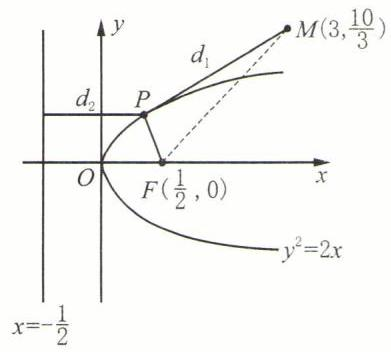
\includegraphics[width=0.3\textwidth]{bodyxb/src/bo_d20cdrf7aajc73bfmvhg_75_328_795_391_352_0.jpg}
\end{center}


(第 167 题)

\begin{center}
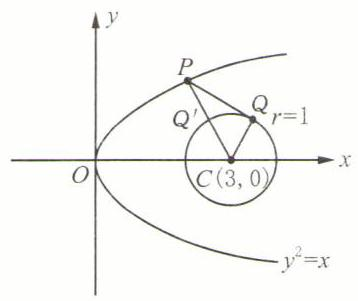
\includegraphics[width=0.3\textwidth]{bodyxb/src/bo_d20cdrf7aajc73bfmvhg_75_828_844_358_301_0.jpg}
\end{center}


(第 168 题)

168. D 提示: 将抛物线方程代入圆的方程,消去 $y$ ,整理得 ${x}^{2} - {5x} + 8 = 0,\Delta  =  - 7 < 0$ ,可见圆在抛物线内. 如图,记圆的圆心为 $C\left( {3,0}\right)$ ,其半径为 $r = 1$ ,线段 ${CP}$ 与圆 $C$ 交于点 ${Q}^{\prime }.\;\because \left| {CP}\right|  - \left| {CQ}\right|  \leq  \left| {QP}\right| ,\therefore \left| {PQ}\right|$ 最小时,点 $Q$ 一定

与点 ${Q}^{\prime }$ 重合. 设 $P\left( {{t}^{2},t}\right)$ ,则 $\left| {P{Q}^{\prime }}\right|  = \left| {PC}\right|  - r = \sqrt{{\left( {t}^{2} - 3\right) }^{2} + {\left( t - 0\right) }^{2}} - 1 = \sqrt{{\left( {t}^{2} - \dfrac{5}{2}\right) }^{2} + \dfrac{11}{4}} - 1,\therefore$ 当 ${t}^{2} =$  $\dfrac{5}{2}$ ,即 $P\left( {\dfrac{5}{2}, \pm  \dfrac{\sqrt{10}}{2}}\right)$ 时, ${\left| P{Q}^{\prime }\right| }_{\min } = \dfrac{1}{2}\left( {\sqrt{11} - 2}\right)$ .

169. (1) ${x}^{2} =  - {16y}$ 提示: 圆心到定点 $F\left( {0, - 4}\right)$ 和定直线 $l : y = 4$ 的距离均为圆的半径,可见圆心轨迹是一条抛物线,其对称轴是过点 $A$ 且垂直于 $l$ 的直线,即 $x$ 轴,故顶点恰为原点. $\therefore \dfrac{p}{2} = 4$ ,所求轨迹方程为 ${x}^{2} =  - {2py} =  - {16y}$ .

(2) $y = 0\left( {x < 0}\right)$ 或 ${y}^{2} = {8x}\left( {x > 0}\right)$ 提示: 设圆心 $A\left( {x,y}\right)$ ,半径为 ${r}_{1}$ . 圆 ${x}^{2} + {y}^{2} - {4x} = 0$ 的圆心为 $B\left( {2,0}\right)$ ,半径为 ${r}_{2}$

$= 2$ . 由题意: $\left\{  {\begin{array}{l} \left| x\right|  = {r}_{1} > 0, \\  \left| {AB}\right|  = \sqrt{{\left( x - 2\right) }^{2} + {y}^{2}} = {r}_{1} + {r}_{2}, \end{array}\;\therefore \;\sqrt{{\left( x - 2\right) }^{2} + {y}^{2}} = \left| x\right|  + 2}\right.$ ,整理得 ${y}^{2} = 4\left( {x + \left| x\right| }\right) ,x \neq  0$ ; 若 $x < 0$ ,则 $y = 0$ ; 若 $x > 0$ ,则 ${y}^{2} = {8x}.\;\therefore$ 所求圆心轨迹方程为 $y = 0\left( {x < 0}\right)$ 或 ${y}^{2} = {8x}\left( {x > 0}\right)$ .

170. (1) ${4x} + y + 3 = 0$ 提示: 设弦的两端分别为 $A\left( {{x}_{1},{y}_{1}}\right) ,B\left( {{x}_{2},{y}_{2}}\right) \left( {{x}_{1} \neq  {x}_{2}}\right.$ ,否则点 $P$ 纵坐标应为 0 ),则 ${y}_{1}^{2} =  - 8{x}_{1}$ , ${y}_{2}^{2} =  - 8{x}_{2}$ ,两式相减,并除以 $\left( {{x}_{1} - {x}_{2}}\right)$ ,得 $\left( {{y}_{1} + {y}_{2}}\right) \dfrac{{y}_{1} - {y}_{2}}{{x}_{1} - {x}_{2}} =  - 8$ ,代入 ${y}_{1} + {y}_{2} = 2,\therefore {k}_{AB} =  - 4,\therefore {l}_{AB}$ : $y - 1 =  - 4\left( {x + 1}\right)$ ,即 ${l}_{AB} : {4x} + y + 3 = 0$ (可以验证该直线确实与抛物线有两个不同公共点).

(2) ${y}^{2} = x + 2$ (在已知抛物线内的部分) 提示: 不难看出,弦 ${AB}$ 的斜率存在,且不为 0 . 记弦 ${AB}$ 的中点为 $C\left( {{x}_{C},{y}_{C}}\right)$ . 方法一: 设 ${l}_{AB} : y = k\left( {x + 2}\right)$ ,代入 ${y}^{2} = {2x}$ ,消去 $y$ ,整理得 ${k}^{2}{x}^{2} + \left( {4{k}^{2} - 2}\right) x + 4{k}^{2} = 0,\Delta  > 0 \Rightarrow  0 < \left| k\right|  < \dfrac{1}{2}$ ,

$\therefore {x}_{1} + {x}_{2} = \dfrac{2}{{k}^{2}} - 4,\therefore \left\{  \begin{array}{l} {x}_{C} = \dfrac{1}{{k}^{2}} - 2, \\  {y}_{C} = \dfrac{1}{k}, \end{array}\right.$ 消去 $k$ ,整理得 ${y}^{2} = x + 2\left( {x > 2\text{ ,即在已知抛物线内的部分 }}\right)$ .

方法二: (点差法) 设弦的两端分别为 $A\left( {{x}_{1},{y}_{1}}\right) ,B\left( {{x}_{2},{y}_{2}}\right) \left( {{x}_{1} \neq  {x}_{2}}\right.$ ,否则弦 ${AB}$ 不可能过(-2,0),则 ${y}_{1}^{2} = 2{x}_{1}$ ,

${y}_{2}^{2} = 2{x}_{2}$ ,两式相减,并除以 $\left( {{x}_{1} - {x}_{2}}\right)$ ,得 $\left( {{y}_{1} + {y}_{2}}\right) \dfrac{{y}_{1} - {y}_{2}}{{x}_{1} - {x}_{2}} = 2$ ,其中 ${y}_{1} + {y}_{2} = 2{y}_{C}$ ,

$\therefore {y}_{C} \cdot  {k}_{AB} = 1$ . 又 ${k}_{AB} = \dfrac{{y}_{C} - 0}{{x}_{C} + 2}$ ,代入 ${y}_{C} \cdot  {k}_{AB} = 1$ ,整理得轨迹方程 ${y}^{2} = x + 2$ (在已知抛物线内的部分).

(3) $x = \dfrac{1}{2}\left( {y > \dfrac{1}{2}}\right.$ ,即在已知抛物线内的部分 $)$ 提示: 设弦的两端分别为 $A\left( {{x}_{1},{y}_{1}}\right) ,B\left( {{x}_{2},{y}_{2}}\right) \left( {{x}_{1} \neq  {x}_{2}}\right.$ ,否则 ${AB}$ 斜率不存在),则 ${y}_{1} = 2{x}_{1}^{2},{y}_{2} = 2{x}_{2}^{2}$ ,两式相减,并除以 $\left( {{x}_{1} - {x}_{2}}\right)$ 得 $\dfrac{{y}_{1} - {y}_{2}}{{x}_{1} - {x}_{2}} = 2\left( {{x}_{1} + {x}_{2}}\right)$ ,代入 $\dfrac{{y}_{1} - {y}_{2}}{{x}_{1} - {x}_{2}} = 2$ ,

$\therefore {x}_{1} + {x}_{2} = 1$ ,可见中点的横坐标始终为 $\dfrac{1}{2},\therefore$ 所求轨迹为 $x = \dfrac{1}{2}\left( {y > \dfrac{1}{2}}\right.$ ,即在已知抛物线内的部分).

171. (1) 由题意,不妨设抛物线为 ${y}^{2} = {2px}\left( {p > 0}\right)$ ,其焦点为 $F\left( {\dfrac{p}{2},0}\right)$ ,淮线为 $x =  - \dfrac{p}{2}$ ,则 ${A}_{1}\left( {-\dfrac{p}{2},{y}_{A}}\right)$ , ${B}_{1}\left( {-\dfrac{p}{2},{y}_{B}}\right) ,\;\therefore \;\vv{F{A}_{1}} = \left( {p, - {y}_{A}}\right) ,\vv{F{B}_{1}} = \left( {p, - {y}_{B}}\right)$ . 直线 ${AB}$ 的斜率不为 0,故设 ${l}_{AB} : {ky} = x - \dfrac{p}{2}$ ,代入 ${y}^{2}$  $= {2px}$ ,消去 $x$ ,整理得 ${y}^{2} - {2pky} - {p}^{2} = 0,\Delta  > 0,\therefore {y}_{A} \cdot  {y}_{B} =  - {p}^{2},\therefore \vv{F{A}_{1}} \cdot  \vv{F{B}_{1}} = {p}^{2} + {y}_{A} \cdot  {y}_{B} = 0$ , $\therefore \angle {A}_{1}F{B}_{1} = {90}^{ \circ  }$ ,证毕.

(2)将直线方程代入抛物线方程,消去 $x$ ,整理得 ${y}^{2} + {4y} - {12} = 0\left( {\Delta  > 0}\right) ,\therefore {y}_{P} \cdot  {y}_{Q} =  - {12}.\vv{OP} \cdot  \vv{OQ} = {x}_{P} \cdot  {x}_{Q} +$  ${y}_{P} \cdot  {y}_{Q} = \dfrac{{\left( {y}_{P} \cdot  {y}_{Q}\right) }^{2}}{12} + {y}_{P} \cdot  {y}_{Q} = 0,\;\therefore \angle {POQ} = {90}^{ \circ  }$ ,证毕.

(3)弦 ${P}_{1}{P}_{2}$ 所在直线的斜率不为 0,设 $M\left( {m,0}\right) \left( {m > 0}\right)$ 及 ${l}_{{P}_{1}{P}_{2}} : {ky} = x - m$ ,代入 ${y}^{2} = {2px}$ ,消去 $x$ ,得 ${y}^{2} - {2pky} -$  $2{p}_{m} = 0\left( {\Delta  > 0}\right) ,\;\therefore \;{y}_{{P}_{1}} + {y}_{{P}_{2}} = 2{p}_{k},{y}_{{P}_{1}} \cdot  {y}_{{P}_{2}} =  - 2{p}_{m},\;\therefore \;{x}_{{P}_{1}} \cdot  {x}_{{P}_{2}} = \left( {k{y}_{{P}_{1}} + m}\right) \left( {k{y}_{{P}_{2}} + m}\right)  = {m}^{2}.$  $\angle {P}_{1}O{P}_{2} = {90}^{ \circ  } \Leftrightarrow  \vv{O{P}_{1}} \cdot  \vv{O{P}_{2}} = {x}_{{P}_{1}} \cdot  {x}_{{P}_{2}} + {y}_{{P}_{1}} \cdot  {y}_{{P}_{2}} = 0$ ,

$\therefore m = {2p}$ ,即存在一点 $M\left( {{2p},0}\right)$ 满足题意,证毕.

172. (1) 设 $B,\left( {\dfrac{{y}_{1}^{2}}{2p},{y}_{1}}\right) ,C\left( {\dfrac{{y}_{1}^{2}}{2p}, - {y}_{1}}\right) ,A\left( {\dfrac{{y}_{2}^{2}}{2p},{y}_{2}}\right) \left( {{y}_{2} \neq   \pm  {y}_{1}}\right)$ ,则 ${l}_{AB} : y - {y}_{2} = \dfrac{2p}{{y}_{1} + {y}_{2}}\left( {x - \dfrac{{y}_{2}^{2}}{2p}}\right)$ ,与 $x$ 轴交于 $D\left( {-\dfrac{{y}_{1}{y}_{2}}{2p},0}\right) ;{l}_{AC} : y - {y}_{2} = \dfrac{2p}{{y}_{2} - {y}_{1}}\left( {x - \dfrac{{y}_{2}^{2}}{2p}}\right)$ ,与 $x$ 轴交于 $E\left( {\dfrac{{y}_{1}{y}_{2}}{2p},0}\right) ,\therefore \vv{OD} =  - \vv{OE}$ ,即抛物线顶点平分线段 ${DE}$ ,证毕.

(2) ${x}_{i} = \dfrac{{y}_{i}^{2}}{2p}\left( {i = 1,2,3}\right) ,\;\therefore \;\left| {CM}\right|  = \left| {\dfrac{{x}_{1} + {x}_{2}}{2} - {x}_{3}}\right|  = \dfrac{1}{2p}\left| {\dfrac{{y}_{1}^{2} + {y}_{2}^{2}}{2} - {y}_{3}^{2}}\right|  = \dfrac{1}{2p}\left| {\dfrac{{y}_{1}^{2} + {y}_{2}^{2}}{2} - {\left( \dfrac{{y}_{1} + {y}_{2}}{2}\right) }^{2}}\right|  =$  $\dfrac{1}{8p}{\left( {y}_{1} - {y}_{2}\right) }^{2} \cdot  {S}_{\bigtriangleup {ABC}} = {S}_{\bigtriangleup {CMB}} + {S}_{\bigtriangleup {CMA}} = \dfrac{1}{2}\left| {CM}\right| \left| {{y}_{1} - {y}_{2}}\right|  = \dfrac{1}{16p}{\left| {y}_{1} - {y}_{2}\right| }^{3}$ ,证毕.

(3) 设 $B\left( {{x}_{0},{y}_{0}}\right)$ . 当 $M$ 的坐标是 $M\left( {\dfrac{p}{2},\dfrac{p}{2}}\right)$ 时,利用 $\vv{BA} =  - \dfrac{4}{3}\vv{AM}$ ,得 $A\left( {{2p} - 3{x}_{0},{2p} - 3{y}_{0}}\right)$ ,由 ${\left( 2p - 3{y}_{0}\right) }^{2} =$  ${2p}\left( {{2p} - 3{x}_{0}}\right)$ 求得 ${x}_{0} = 0,{y}_{0} = 0$ ,于是直线 ${AB}$ 的方程为 $x - y = 0,\left| {AB}\right|  = 2\sqrt{2}p$ . 当 $M$ 的坐标是 $M\left( {\dfrac{p}{2}, - \dfrac{p}{2}}\right)$ 时,直线 ${AB}$ 的方程为 $x + y = 0,\left| {AB}\right|  = 2\sqrt{2}p$ 不变.

(4) 直线 ${PQ}$ 的斜率存在,设为 $k$ 且 $k \neq  0$ . 记 $P\left( {{x}_{1},{y}_{1}}\right) ,Q\left( {{x}_{2},{y}_{2}}\right) \left( {{x}_{1} \neq  {x}_{2}}\right) ,{PQ}$ 的中点为 $C\left( {{x}_{C},{y}_{C}}\right)$ . 则 ${y}_{1}^{2} = {2p}{x}_{1}$ , ${y}_{2}^{2} = {2p}{x}_{2}$ ,两式相减,并除以 $\left( {{x}_{1} - {x}_{2}}\right)$ ,得 $\left( {{y}_{1} + {y}_{2}}\right) \dfrac{{y}_{1} - {y}_{2}}{{x}_{1} - {x}_{2}} = {2p}$ ,代入 ${y}_{1} + {y}_{2} = 2{y}_{C}$ 和 $\dfrac{{y}_{1} - {y}_{2}}{{x}_{1} - {x}_{2}} = k$ ,得 ${y}_{C} = \dfrac{p}{k}$ . 线段 ${PQ}$ 的垂直平分线为 $y - {y}_{C} =  - \dfrac{1}{k}\left( {x - {x}_{C}}\right)$ ,与 $x$ 轴交于 $R\left( {k{y}_{C} + {x}_{C},0}\right)$ ,即 $R\left( {p + {x}_{C},0}\right)$ ,

$\therefore \left| {FR}\right|  = {x}_{C} + \dfrac{p}{2}$ . 另一方面,由双曲线的性质, $\left| {PQ}\right|  = \left| {FP}\right|  + \left| {FQ}\right|  = \left( {{x}_{1} + \dfrac{p}{2}}\right)  + \left( {{x}_{2} + \dfrac{p}{2}}\right)  = 2{x}_{C} + p$ ,

$\therefore \left| {FR}\right|  = \dfrac{1}{2}\left| {PQ}\right|$ ,证毕.

(5) 方法一: (标点法) 设 $A\left( {{x}_{1},\dfrac{{x}_{1}^{2}}{2p}}\right) ,B\left( {{x}_{2},\dfrac{{x}_{2}^{2}}{2p}}\right)$ ,则由 ${OA}\bot {OB}$ 得 ${x}_{1}{x}_{2} =  - 4{p}^{2},{\left| OA\right| }^{2} = \dfrac{{x}_{1}^{2}}{4{p}^{2}}\left( {{x}_{1}^{2} + 4{p}^{2}}\right) ,{\left| OB\right| }^{2} =$  $\dfrac{{x}_{2}^{2}}{4{p}^{2}}\left( {{x}_{2}^{2} + 4{p}^{2}}\right)$ ,于是 $S = \dfrac{1}{2}\left| {OA}\right|$ . $\left| {OB}\right|  = \dfrac{\left| {x}_{1}{x}_{2}\right| }{8{p}^{2}}\sqrt{\left( {{x}_{1}^{2} + 4{p}^{2}}\right) \left( {{x}_{2}^{2} + 4{p}^{2}}\right) } = \dfrac{1}{2}\sqrt{{32}{p}^{4} + 4{p}^{2}\left( {{x}_{1}^{2} + {x}_{2}^{2}}\right) } \geq$  $\dfrac{1}{2}\sqrt{{32}{p}^{4} + 8{p}^{2}\left| {{x}_{1}{x}_{2}}\right| } = 4{p}^{2}.\;\therefore$ 当 $\left| {x}_{1}\right|  = \left| {x}_{2}\right|$ ,即 $A\left( {{2p},{2p}}\right) ,B\left( {-{2p},{2p}}\right)$ 时, ${S}_{\text{ 最小值 }} = 4{p}^{2}$ .

方法二: ${OA}$ , ${OB}$ 的斜率都存在,且不为 0 . 设 ${l}_{OA} : y = {kx}\left( {k > 0}\right)$ ,代入 ${x}^{2} = {2py}$ ,可得 $A\left( {{2pk},{2p}{k}^{2}}\right)$ ,故 $\left| {OA}\right|  =$  ${2pk}\sqrt{1 + {k}^{2}}$ ; 用 $- \dfrac{1}{k}$ 代替 $k$ ,得 $\left| {OB}\right|  = {2p}\dfrac{1}{k}\sqrt{1 + \dfrac{1}{{k}^{2}}}.\;\therefore \;{S}_{\bigtriangleup {AOB}} = \dfrac{1}{2}\left| {OA}\right| \left| {OB}\right|  = 2{p}^{2}\sqrt{{k}^{2} + \dfrac{1}{{k}^{2}} + 2} \geq$

$2{p}^{2}\sqrt{2\sqrt{{k}^{2} \cdot  \dfrac{1}{{k}^{2}}} + 2} = 4{p}^{2}$ ,当且仅当 ${k}^{2} = \dfrac{1}{{k}^{2}}\left( {k > 0}\right)$ ,即 $k = 1$ 时等号成立,此时 $A\left( {{2p},{2p}}\right)$ , $B\left( {-{2p},{2p}}\right)$ .

方法三:(极坐标) 以 $O$ 为极点,射线 ${Ox}$ 为极轴建立的极坐标系中,抛物线的极坐标方程为 $\rho  = \dfrac{{2p}\sin \theta }{{\cos }^{2}\theta }$  $\left( {\theta  \in  \left\lbrack  {0,\dfrac{\pi }{2}}\right)  \cup  \left( {\dfrac{\pi }{2},\pi }\right\rbrack  }\right)$ ,设 $\angle {AOx} = \varphi \left( {\varphi  \in  \left( {0,\dfrac{\pi }{2}}\right) }\right)$ ,则 $\angle {BOx} = \varphi  + \dfrac{\pi }{2}$ ,代入极坐标方程,得 $\left| {OA}\right|  = \dfrac{{2p}\sin \varphi }{{\cos }^{2}\varphi }$ , $\left| {OB}\right|  = \dfrac{{2p}\cos \varphi }{{\sin }^{2}\varphi },\;\therefore \;{S}_{\bigtriangleup {AOB}} = \dfrac{1}{2}\left| {OA}\right| \left| {OB}\right|  = \dfrac{2{p}^{2}}{\sin \varphi \cos \varphi } = \dfrac{4{p}^{2}}{\sin {2\varphi }} \geq  4{p}^{2}$ ,等号当且仅当 $\varphi  = \dfrac{\pi }{4}$ 时成立,此时 $A\left( {{2p},{2p}}\right) ,B\left( {-{2p},{2p}}\right)$ .

(6)由题意,设直线 ${AB}$ 的方程为 $y = x + b$ ,代入 ${y}^{2} = {8x}$ ,消去 $x$ ,得 ${y}^{2} - {8y} + {8b} = 0,\Delta  = {64} - {32b}$ , $\therefore \left| {AB}\right|  =$  $\sqrt{2}\left| {{y}_{1} - {y}_{2}}\right|  = \sqrt{2}\sqrt{\Delta } = 8\sqrt{2 - b} = 8\sqrt{5},\therefore b =  - 3,{l}_{AB} : x - y - 3 = 0$ . 焦点坐标为 $F\left( {2,0}\right)$ ,到 ${l}_{AB}$ 的距离为 $h$  $= \dfrac{\left| 2 - 0 - 3\right| }{\sqrt{2}} = \dfrac{\sqrt{2}}{2},\;\therefore \;{S}_{\bigtriangleup {FAB}} = \dfrac{1}{2}\left| {AB}\right|  \cdot  h = 2\sqrt{10}.{S}_{\bigtriangleup {FAB}} = \dfrac{1}{2}\left| {FA}\right| \left| {FB}\right| \sin \angle {AFB}$ ,由抛物线的性质,其中 $\left| {FA}\right| \left| {FB}\right|  = \left( {{x}_{A} + \dfrac{p}{2}}\right) \left( {{x}_{B} + \dfrac{p}{2}}\right)  = \left( {{x}_{A} + 2}\right) \left( {{x}_{B} + 2}\right)  = \left( {{y}_{A} + 5}\right) \left( {{y}_{B} + 5}\right)  = {y}_{A}{y}_{B} + 5\left( {{y}_{A} + {y}_{B}}\right)  + {25}$ ,由韦达定理, ${y}_{A} + {y}_{B} = 8,{y}_{A}{y}_{B} = {8b} =  - {24}$ ,

$\therefore \left| {FA}\right| \left| {FB}\right|  = {41},\;\therefore \;\sin \angle {AFB} = \dfrac{4\sqrt{10}}{41}$ .

173. (1) 由题意,设 ${l}_{CD} : y = x + t$ ,则平行直线 ${AB},{CD}$ 间的距离为 $\dfrac{\left| 4 - t\right| }{\sqrt{2}}$ ,即为正方形的边长. 另一方面,将 ${l}_{CD} : y = x + t$ 代入 ${y}^{2} = x$ ,消去 $y$ ,整理得 ${x}^{2} + \left( {{2t} - 1}\right) x + {t}^{2} = 0,\Delta  = 1 - {4t}$ ,弦长 $\left| {CD}\right|  = \sqrt{1 + {k}_{CD}^{2}} \cdot  \sqrt{\Delta } = \sqrt{2} \cdot  \sqrt{1 - {4t}} =$  $\dfrac{\left| 4 - t\right| }{\sqrt{2}}$ ,由关于 $t$ 的方程解得 $t =  - 2$ 或 $t =  - 6\left( {\Delta \text{ 均大于 0 }}\right)$ ,对应的正方形的边长为 $3\sqrt{2}$ 或 $5\sqrt{2}$ .

(2)方法一:将 ${MN}$ 的方程 $y = x + m$ 代入 ${y}^{2} = {4x}$ ,得 $\left| {MN}\right|  = 4\sqrt{2} \cdot  \sqrt{1 - m}$ ,点 $P$ 到 ${MN}$ 的距离 $d = \dfrac{\left| m + {11}\right| }{\sqrt{2}},S =$  $2\sqrt{1 - m}\left| {m + {11}}\right|$ ,再利用不等式性质得最大值 32. 方法二:设直线 ${MN}$ 与 $x$ 轴交于点 $T\left( {t,0}\right) \left( {0 < t < {11}}\right)$ ,则 ${l}_{MN}$ : $y = x - t$ ,代入 ${y}^{2} = {4x}$ ,消去 $x$ ,得: ${y}^{2} - {4y} - {4t} = 0,\;\therefore \;\left| {{y}_{M} - {y}_{N}}\right|  = \sqrt{\Delta } = 4\sqrt{t + 1}.{S}_{\bigtriangleup {PMN}} = {S}_{\bigtriangleup {TPM}} + {S}_{\bigtriangleup {TPN}}$  $= \dfrac{1}{2}\left| {TP}\right| \left| {{y}_{M} - {y}_{N}}\right|  = 2 \cdot  \left( {{11} - t}\right)  \cdot  \sqrt{t + 1} = 4 \cdot  \sqrt{\dfrac{{11} - t}{2}} \cdot  \sqrt{\dfrac{{11} - t}{2}} \cdot  \sqrt{t + 1}$ ,利用不等式 ${abc} \leq$  ${\left( \dfrac{{a}^{2} + {b}^{2} + {c}^{2}}{3}\right) }^{\dfrac{3}{2}}\left( {a,b,c > 0}\right)$ ,得 ${S}_{\bigtriangleup {PMN}} \leq  4 \cdot  {\left( \dfrac{12}{3}\right) }^{\dfrac{3}{2}} = {32}$ ,当且仅当 $\dfrac{{11} - t}{2} = t + 1$ ,即 $t = 3,{l}_{MN} : x - y - 3 = 0$ 时等号成立.

174. (1) 记弦 ${PQ}$ 的中点为 $M\left( {{x}_{M},{y}_{M}}\right)$ 由题意,弦 ${PQ}$ 的斜率为 1 . 方法一: 设 ${l}_{PQ} : y = x + b$ ,代入 ${y}^{2} = x$ ,消去 $y$ ,整理得 ${x}^{2}$  $+ \left( {{2b} - 1}\right) x + {b}^{2} = 0,\Delta  = 1 - {4b},{x}_{M} = \dfrac{{x}_{1} + {x}_{2}}{2} = \dfrac{1}{2} - b,{y}_{M} = {x}_{M} + b = \dfrac{1}{2}$ . 将 $M\left( {\dfrac{1}{2} - b,\dfrac{1}{2}}\right)$ 代入 $x + y - 2 = 0$ ,得 $b =  - 1\left( {\Delta  > 0}\right)$ . 故 $\left| {PQ}\right|  = \sqrt{1 + {k}_{PQ}^{2}}\sqrt{\Delta } = \sqrt{2}\sqrt{1 - {4b}} = \sqrt{10}$ ,点 $O$ 到 ${l}_{PQ} : x - y - 1 = 0$ 的距离为 $h = \dfrac{1}{\sqrt{2}}$ ,

$\therefore {S}_{\bigtriangleup {OPQ}} = \dfrac{1}{2}\left| {PQ}\right|  \cdot  h = \dfrac{\sqrt{5}}{2}$ . 方法二: (点差法) 设 $P\left( {{x}_{1},{y}_{1}}\right) ,Q\left( {{x}_{2},{y}_{2}}\right)$ ,则有 ${y}_{1}^{2} = {x}_{1},{y}_{2}^{2} = {x}_{2}$ ,两式相减得 $\left( {y}_{1}\right.$  $\left. {+{y}_{2}}\right)  \cdot  \left( {{y}_{1} - {y}_{2}}\right)  = {x}_{1} - {x}_{2}$ ,其中 $\dfrac{{y}_{1} - {y}_{2}}{{x}_{1} - {x}_{2}} = 1,\;\therefore \;{y}_{M} = \dfrac{{y}_{1} + {y}_{2}}{2} = \dfrac{1}{2}$ ,代入 $x + y - 2 = 0$ ,得 $M\left( {\dfrac{3}{2},\dfrac{1}{2}}\right)$ ,

$\therefore {l}_{PQ} : y - \dfrac{1}{2} = x - \dfrac{3}{2}$ ,即 ${l}_{PQ} : x - y - 1 = 0.{PQ}$ 与 $x$ 轴交于 $R\left( {1,0}\right)$ ,故 $\left| {OR}\right|  = 1$ ; 将 ${l}_{PQ} : x - y - 1 = 0$ 代入 ${y}^{2}$  $= x$ ,消去 $x$ ,得 ${y}^{2} - y - 1 = 0,\Delta  = 5 > 0,\therefore \left| {{y}_{1} - {y}_{2}}\right|  = \sqrt{\Delta } = \sqrt{5},\therefore {S}_{\bigtriangleup {OPQ}} = {S}_{\bigtriangleup {ORP}} + {S}_{\bigtriangleup {ORQ}} = \dfrac{1}{2}\left| {OR}\right|$ . $\left| {{y}_{1} - {y}_{2}}\right|  = \dfrac{\sqrt{5}}{2}.$

(2)显然, $k \neq  0$ . 记 $A\left( {{x}_{1},{y}_{1}}\right) ,B\left( {{x}_{2},{y}_{2}}\right) ,{AB}$ 的中点为 $M\left( {{x}_{M},{y}_{M}}\right)$ . 由 ${y}_{1}^{2} = {x}_{1},{y}_{2}^{2} = {x}_{2}$ ,两式相减可得 $\left( {{y}_{1} + {y}_{2}}\right) \left( {{y}_{1} - }\right.$  $\left. {y}_{2}\right)  = {x}_{1} - {x}_{2},\dfrac{{y}_{1} - {y}_{2}}{{x}_{1} - {x}_{2}} =  - \dfrac{1}{k},\;\therefore \;{y}_{1} + {y}_{2} =  - k,\;\therefore \;{y}_{M} =  - \dfrac{k}{2}$ ,代入 $y - 1 = k\left( {x - 1}\right)$ ,得 $M\left( {\dfrac{1}{2} - \dfrac{1}{k}, - \dfrac{k}{2}}\right)$ . 方法一:由点 $M$ 在抛物线内,得 ${\left( -\dfrac{k}{2}\right) }^{2} < \dfrac{1}{2} - \dfrac{1}{k} \Leftrightarrow  {k}^{2} < 2 - \dfrac{4}{k}$ ,两边乘以 ${k}^{2}$ (注意不是 $k$ ),整

理得 $k\left( {k + 2}\right) \left( {{k}^{2} - {2k} + 2}\right)  < 0$ ,注意到 ${k}^{2} - {2k} + 2 > 0,\therefore  - 2 < k < 0$ . 方法二: ${x}_{M} = \dfrac{{x}_{1} + {x}_{2}}{2} = \dfrac{{y}_{1}^{2} + {y}_{2}^{2}}{2} =$  $\dfrac{{\left( {y}_{1} + {y}_{2}\right) }^{2} - 2{y}_{1}{y}_{2}}{2}$ ,可求得 ${y}_{1}{y}_{2} = \dfrac{1}{2}\left( {{k}^{2} - 1 + \dfrac{2}{k}}\right) ,\therefore {y}_{1},{y}_{2}$ 是方程 ${t}^{2} + {kt} + \dfrac{1}{2}\left( {{k}^{2} - 1 + \dfrac{2}{k}}\right)  = 0$ 的两个实根,由 $\Delta  > 0$ 可以得到 ${k}^{2} < 2 - \dfrac{4}{k}$ ,与方法一的不等式相同, $\therefore  - 2 < k < 0$ .

175. (1) 由题意, $\left| {PA}\right|  = \sqrt{{\left( x - a\right) }^{2} + {y}^{2}} = \sqrt{{x}^{2} - {2ax} + {a}^{2} + {2x}} = \sqrt{{\left\lbrack  x - \left( a - 1\right) \right\rbrack  }^{2} + \left( {{2a} - 1}\right) }$ . 根据二次函数的性质,当 $a$  $- 1 > 0$ ,即 $a > 1$ 时, ${\left| PA\right| }_{\min } = \sqrt{{2a} - 1}$ ,此时 $P\left( {a - 1, \pm  \sqrt{2\left( {a - 1}\right) }}\right)$ ; 当 $a - 1 \leq  0$ ,即 $a \leq  1$ 时, ${\left| PA\right| }_{\min } =$  $\sqrt{{\left\lbrack  0 - \left( a - 1\right) \right\rbrack  }^{2} + \left( {{2a} - 1}\right) } = \left| a\right|$ ,此时 $P\left( {0,0}\right) .\;\therefore \;f\left( a\right)  = \left\{  \begin{array}{l} \left| a\right| ,a \leq  1, \\  \sqrt{{2a} - 1},a > 1. \end{array}\right.$

(2)分段讨论. ①当 $\dfrac{1}{3} \leq  a \leq  1$ 时, $f\left( a\right)  = \left| a\right|  = a$ 是严格增函数,故 $f{\left( a\right) }_{\max } = f\left( 1\right)  = 1,f{\left( a\right) }_{\min } = f\left( \dfrac{1}{3}\right)  = \dfrac{1}{3}$ ；②当 1 $< a \leq  5$ 时, $f\left( a\right)  = \sqrt{{2a} - 1}$ 是严格增函数,故 $f{\left( a\right) }_{\max } = f\left( 5\right)  = 3,f{\left( a\right) }_{\min }$ 不存在,但 $f\left( a\right)  > \sqrt{2 - 1} = 1$ . 综上,当 $\dfrac{1}{3} \leq  a \leq  5$ 时, $f{\left( a\right) }_{\max } = f\left( 5\right)  = 3;f{\left( a\right) }_{\min } = f\left( \dfrac{1}{3}\right)  = \dfrac{1}{3}$ .

176. (1) 由题意, ${F}_{2}\left( {1,0}\right)$ ,故椭圆的焦点在 $x$ 轴上,且有 $c = \sqrt{9 - m} = 1,\therefore m = 8$ .

(2) ${F}_{1}\left( {-1,0}\right)$ ,又记 $\left| {P{F}_{1}}\right|  = q$ , $\left| {P{F}_{2}}\right|  = r$ , $\left| {{F}_{1}{F}_{2}}\right|  = s = {2c}$ ,将抛物线方程代入椭圆 $\dfrac{{x}^{2}}{9} + \dfrac{{y}^{2}}{8} = 1$ ,整理得 $2{x}^{2} + {9x} - {18}$  $= 0,x > 0,\therefore {x}_{P} = \dfrac{3}{2}$ . 由抛物线的性质, $r = {x}_{P} + \dfrac{p}{2} = \dfrac{5}{2}$ ,由椭圆的性质, $q + r = 6,\therefore q = \dfrac{7}{2}$ . 方法一: (根据射影求解) 点 $P$ 在 $x$ 轴上的射影是 ${P}^{\prime }\left( {\dfrac{3}{2},0}\right)$ ,在 ${F}_{1}{F}_{2}$ 的延长线上, $\therefore \beta$ 是钝角. 又 $\left| {{F}_{1}{P}^{\prime }}\right|  = \dfrac{5}{2}$ , $\left| {{F}_{2}{P}^{\prime }}\right|  = \dfrac{1}{2},\;\therefore \;\cos \alpha  = \dfrac{\left| {F}_{1}{P}^{\prime }\right| }{\left| {F}_{1}P\right| } = \dfrac{\dfrac{5}{2}}{q} = \dfrac{5}{7},\cos \beta  =  - \dfrac{\left| {F}_{2}{P}^{\prime }\right| }{\left| {F}_{2}P\right| } =  - \dfrac{\dfrac{1}{2}}{r} =  - \dfrac{1}{5},\;\therefore \;\cos \alpha  \cdot  \cos \beta  =  - \dfrac{1}{7}$ . 方法二: (根据余弦定理) $\cos \alpha  = \dfrac{{q}^{2} + {s}^{2} - {r}^{2}}{2qs} = \dfrac{{s}^{2} + {2a}\left( {q - r}\right) }{2qs},\cos \beta  = \dfrac{{r}^{2} + {s}^{2} - {q}^{2}}{2rs} = \dfrac{{s}^{2} - {2a}\left( {q - r}\right) }{2rs},\;\therefore \;\cos \alpha  \cdot  \cos \beta  =$  $\dfrac{{s}^{4} - 4{a}^{2}{\left( q - r\right) }^{2}}{4{s}^{2}{qr}} = \dfrac{4{c}^{4} - {a}^{2}{\left( q - r\right) }^{2}}{4{c}^{2}{qr}}$ . 代入 $c = 1,a = 3,q = \dfrac{7}{2},r = \dfrac{5}{2}$ ,得 $\cos \alpha  \cdot  \cos \beta  =  - \dfrac{1}{7}$ .

(3) 方法一:根据(2)方法一中所得的 $\cos \alpha  = \dfrac{5}{7}$ ,可得 $\sin \alpha  = \dfrac{2\sqrt{6}}{7},\therefore {S}_{\bigtriangleup P{F}_{1}{F}_{2}} = \dfrac{1}{2}\left| {P{F}_{1}}\right| \left| {{F}_{1}{F}_{2}}\right| \sin \alpha  = {cq}\sin \alpha  = \sqrt{6}$ (也可通过 $\cos \beta$ 求解). 方法二:不难求得 $\left| {y}_{P}\right|  = \sqrt{6}$ ,

$\therefore {S}_{\bigtriangleup P{F}_{1}{F}_{2}} = \dfrac{1}{2}\left| {{F}_{1}{F}_{2}}\right| \left| {y}_{P}\right|  = c \cdot  \left| {y}_{P}\right|  = \sqrt{6}$ . 方法三: (海伦公式) 我们注意到, $\bigtriangleup P{F}_{1}{F}_{2}$ 的三边长 $q = \dfrac{7}{2},r =$  $\dfrac{5}{2},s = 2$ ,故使用海伦公式: ${S}_{\bigtriangleup P{F}_{1}{F}_{2}} = \sqrt{t\left( {t - q}\right) \left( {t - r}\right) \left( {t - s}\right) } = \sqrt{6}$ ,其中 $t = \dfrac{q + r + s}{2} = 4$ .

177. (1) 记 $P\left( {{x}_{1},{y}_{1}}\right) ,Q\left( {{x}_{2},{y}_{2}}\right) \left( {{x}_{1},{x}_{2} \neq  0}\right)$ . 方法一: 由 $\vv{OP}\bot \vv{OQ} \Leftrightarrow  \vv{OP} \cdot  \vv{OQ} = 0,\;\therefore {x}_{1}{x}_{2} + {y}_{1}{y}_{2} = {x}_{1}{x}_{2} + {x}_{1}^{2}{x}_{2}^{2} = 0$ , $\therefore {x}_{2} =  - \dfrac{1}{{x}_{1}}$ . 由 $\vv{OR} = \vv{OP} + \vv{OQ}$ ,可知 $\left\{  {\begin{array}{l} {x}_{R} = {x}_{1} - \dfrac{1}{{x}_{1}}, \\  {y}_{R} = {y}_{1} + {y}_{2} = {x}_{1}^{2} + \dfrac{1}{{x}_{1}^{2}}, \end{array}\left( {{x}_{1} \neq  0}\right) }\right.$ 消去 ${x}_{1},\therefore$ 点 $R$ 的轨迹方程为 $y =$  ${x}^{2} + 2$ . 方法二: 易知, ${OP},{OQ}$ 的斜率均存在,且不为 0 . 设 ${l}_{OP} : y = {kx}\left( {k \neq  0}\right)$ ,则 ${l}_{OQ} : y =  - \dfrac{1}{k}x$ ,分别代入 $y = {x}^{2}$ , 可得 $P\left( {k,{k}^{2}}\right)$ 和 $Q\left( {-\dfrac{1}{k},\dfrac{1}{{k}^{2}}}\right)$ . 由 $\vv{OR} = \vv{OP} + \vv{OQ}$ ,可知 $\left\{  {\begin{array}{l} {x}_{R} = k - \dfrac{1}{k}, \\  {y}_{R} = {k}^{2} + \dfrac{1}{{k}^{2}} \end{array}\left( {k \neq  0}\right) }\right.$ ,消去 $k,\therefore$ 点 $R$ 的轨迹方程为 $y$  $= {x}^{2} + 2$ .

(2) $O{P}_{1}$ 和 $O{P}_{2}$ 的斜率均存在,且不为 0 . 方法一；设 ${l}_{O{P}_{1}} : y = {kx}\left( {k \neq  0}\right)$ ,则 ${l}_{O{P}_{2}} : y =  - \dfrac{1}{k}x$ ,分别代入 ${y}^{2} = {2px}$ ,可得 ${P}_{1}\left( {\dfrac{2p}{{k}^{2}},\dfrac{2p}{k}}\right)$ 和 ${P}_{2}\left( {{2p}{k}^{2}, - {2pk}}\right)$ ,于是以 $O{P}_{1}$ 和 $O{P}_{2}$ 为直径的圆的方程分别为 ${x}^{2} + {y}^{2} - \dfrac{2p}{{k}^{2}}x - \dfrac{2p}{k}y = 0$ 和 ${x}^{2} +$  ${y}^{2} - {2p}{k}^{2}x + {2pky} = 0$ ,两方程相减,得 ${OP}$ 所在直线方程为 $y = \dfrac{{k}^{2} - \dfrac{1}{{k}^{2}}}{k + \dfrac{1}{k}}x = \left( {k - \dfrac{1}{k}}\right) x = {tx}\left( {t = k - \dfrac{1}{k} \in  \mathbf{R}}\right)$ ,代入

以 $O{P}_{1}$ (或 $O{P}_{2}$ )为直径的圆的方程,注意到 $P\left( {{x}_{P},{y}_{P}}\right)  \neq  \left( {0,0}\right)$ ,

$\therefore \left\{  \begin{array}{l} {x}_{P} = \dfrac{2pt}{1 + {t}^{2}}, \\  {y}_{P} = \dfrac{2pt}{1 + {t}^{2}}, \end{array}\right.$ 消去 $t$ ,即得点 $P$ 的轨迹是一个圆: ${\left( x - p\right) }^{2} + {y}^{2} = {p}^{2}$ ,即 ${x}^{2} + {y}^{2} - {2px} = 0(x \neq  0$ ,在已知抛物线内的部分). 方法二: 设 ${P}_{1}\left( {{x}_{1},{y}_{1}}\right) ,{P}_{2}\left( {{x}_{2},{y}_{2}}\right) \left( {{x}_{1},{x}_{2},{y}_{1},{y}_{2} \neq  0,{y}_{1} \neq  {y}_{2}}\right)$ ,由 $\vv{OP} \bot  \vv{OQ} \Leftrightarrow  \vv{OP} \cdot  \vv{OQ} = 0$ ,

$\therefore {x}_{1}{x}_{2} + {y}_{1}{y}_{2} = \dfrac{{y}_{1}^{2}{y}_{2}^{2}}{4{p}^{2}} + {y}_{1}{y}_{2} = 0,\therefore {y}_{1}{y}_{2} =  - 4{p}^{2}$ . 以 $O{P}_{1}$ 和 $O{P}_{2}$ 为直径的圆的方程分别为 ${x}^{2} + {y}^{2} - {x}_{1}x$  $- {y}_{1}y = 0$ 和 ${x}^{2} + {y}^{2} - {x}_{2}x - {y}_{2}y = 0$ ,两方程相减,得 ${OP}$ 所在直线方程为 $\left( {{x}_{2} - {x}_{1}}\right) x + \left( {{y}_{2} - {y}_{1}}\right) y = 0$ ,即 $y =$  $- \dfrac{{x}_{2} - {x}_{1}}{{y}_{2} - {y}_{1}}x =  - \dfrac{{y}_{1} + {y}_{2}}{2p}x = \operatorname{tr}\left( {t =  - \dfrac{{y}_{1} + {y}_{2}}{2p} = \dfrac{2p}{{y}_{1}} - \dfrac{{y}_{1}}{2p} \in  \mathbf{R}}\right)$ ,再代入以 $O{P}_{1}$ (或 $O{P}_{2}$ )为直径的圆方程,注意到 $P\left( {{x}_{P},{y}_{P}}\right)  \neq  \left( {0,0}\right) ,\;\therefore \;{x}_{P} = \dfrac{{x}_{1} + {y}_{1}t}{1 + {t}^{2}} = \dfrac{\dfrac{{y}_{1}^{2}}{2p} - {y}_{1}\dfrac{{y}_{1} + {y}_{2}}{2p}}{1 + {t}^{2}} = \dfrac{-{y}_{1}{y}_{2}}{{2p}\left( {1 + {t}^{2}}\right) } = \dfrac{2p}{1 + {t}^{2}}$ ,代入 $t = \dfrac{{y}_{P}}{{x}_{P}}$ ,整理得 ${x}^{2} + {y}^{2} -$  ${2px} = 0$ (已知抛物线内的部分).

178. (1) $\left| {AB}\right|  = 4$ ,由题意, $\left| {PA}\right|  + \left| {PB}\right|  = {10} - \left| {AB}\right|  = 6$ ,故动点 $P$ 位于焦点在 $x$ 轴的椭圆 $\dfrac{{x}^{2}}{{a}^{2}} + \dfrac{{y}^{2}}{{b}^{2}} = 1$ 上,且 $A,B,P$ 三点不共线. 又 $a = \dfrac{6}{2} = 3,c = \dfrac{4}{2} = 2,b = \sqrt{{a}^{2} - {c}^{2}} = \sqrt{5},\therefore$ 点 $P$ 的轨迹为 $\dfrac{{x}^{2}}{9} + \dfrac{{y}^{2}}{5} = 1\left( {y \neq  0}\right)$ .

(2)由题意, $\left| {PA}\right|  = {r}_{P} + {r}_{C} = \left| {PB}\right|  + 1,\therefore \left| {PA}\right|  - \left| {PB}\right|  = 1$ ,故动点 $P$ 位于焦点在 $x$ 轴的双曲线 $\dfrac{{x}^{2}}{{a}^{2}} - \dfrac{{y}^{2}}{{b}^{2}} = 1$ 的右支上,又 $a = \dfrac{1}{2},c = \dfrac{4}{2} = 2,b = \sqrt{{c}^{2} - {a}^{2}} = \dfrac{\sqrt{15}}{2},\therefore$ 点 $P$ 的轨迹为 $4{x}^{2} - \dfrac{4{y}^{2}}{15} = 1\left( {x \geq  \dfrac{1}{2}}\right)$ .

(3) 设 $P\left( {x,y}\right)$ ,圆 $P$ 的半径为 $r$ . 由题意, $\left\{  \begin{array}{l} \left| {PA}\right|  = \sqrt{{\left( x + 2\right) }^{2} + {y}^{2}} = r + {r}_{C} = r + 1, \\  r = \left| {x - 1}\right| , \end{array}\right.$

$\therefore \sqrt{{\left( x + 2\right) }^{2} + {y}^{2}} = \left| {x - 1}\right|  + 1$ ,两边平方,整理得 ${y}^{2} = 2\left| {x - 1}\right|  - {6x} - 2$ . 若 $x > 1$ ,此时 ${y}^{2} =  - 4\left( {x + 1}\right)  < 0$ ,没有满足条件的点; $\therefore x \leq  1$ ,此时 ${y}^{2} =  - {8x}$ . 综上,点 $P$ 的轨迹是抛物线 ${y}^{2} =  - {8x}$ .

179. $\dfrac{7 - \sqrt{17}}{2}$ . 将抛物线方程代入圆的方程,消去 $x$ ,整理得 ${x}^{2} + \left( {p - 4}\right) x + 1 = 0$ ,该方程需有两个不同的正实根,

$\therefore \left\{  {\begin{array}{l} \Delta  = {p}^{2} - {8p} + {12} > 0, \\  {x}_{1} + {x}_{2} = 4 - p > 0, \\  {x}_{1}{x}_{2} = 1 > 0, \end{array}\therefore \;0 < p < 2}\right.$ . 又, ${x}_{M} = \dfrac{{x}_{1} + {x}_{2}}{2} = \dfrac{4 - p}{2},{y}_{M} = \dfrac{{y}_{1} + {y}_{2}}{2} = \dfrac{\sqrt{p}}{2}\left( {\sqrt{{x}_{1}} + \sqrt{{x}_{2}}}\right)  = \dfrac{\sqrt{p}}{2}$ . $\sqrt{{x}_{1} + {x}_{2} + 2\sqrt{{x}_{1}{x}_{2}}} = \dfrac{\sqrt{p\left( {6 - p}\right) }}{2}$ . 将 $\left( {{x}_{M},{y}_{M}}\right)$ 代入 $y = x$ ,整理得: ${p}^{2} - {7p} + 8 = 0$ ,注意到 $0 < p < 2$ , $\therefore \;p = \dfrac{7 - \sqrt{17}}{2}$ .

180. 若(x, y)是抛物线和椭圆的一个公共点,那么(-x, y)也一定是两条曲线的公共点. 现已知抛物线和椭圆的公共点个数为 3 个 (奇数个), 故至少有一个公共点的横坐标是 0 . 对于椭圆, 该点为 $\left( {0, \pm  b}\right)$ ；但对于抛物线,该点是唯一的,即顶点 $A\left( {0,m}\right)$ . 结合抛物线 $y = {x}^{2} + m$ (开口向上) 经过椭圆在 $x$ 轴上的两个焦点,可知: 横坐标是 0 的公共点是唯一的,故 $b =  - m,m$  $< 0$ . 两条曲线的相对位置如图所示. 将焦点 $\left( {\pm c,0}\right)$ 代入抛物线,得 ${c}^{2} =  - m,\;\therefore \;{a}^{2} = {b}^{2}$  $+ {c}^{2} = {m}^{2} - m,\therefore$ 椭圆方程为 $\dfrac{{x}^{2}}{{m}^{2} - m} + \dfrac{{y}^{2}}{{m}^{2}} = 1$ ,代入 $y = {x}^{2} + m$ ,消去 $x$ ,整理得(m - 1) ${y}^{2} + {my} - {m}^{3} = 0$ 解得 ${y}_{1} = m,{y}_{2} = \dfrac{{m}^{2}}{1 - m}\left( {{y}_{2} < b}\right.$ 必成立 $),\therefore \left| {{y}_{2} - {y}_{1}}\right|  = \dfrac{2{m}^{2} - m}{1 - m}$ ,

\begin{center}
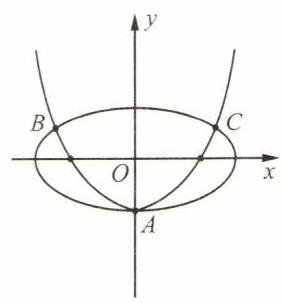
\includegraphics[width=0.2\textwidth]{bodyxb/src/bo_d20cdrf7aajc73bfmvhg_79_1155_1515_284_303_0.jpg}
\end{center}


(第 180 题)

$\therefore$ 抛物线与椭圆在 $x$ 轴上方的公共点为 $B\left( {-{x}_{2},{y}_{2}}\right)$ 和 $C\left( {{x}_{2},{y}_{2}}\right)$ ,其中 ${x}_{2} =$  $\sqrt{\dfrac{2{m}^{2} - m}{1 - m}} \cdot  {S}_{\bigtriangleup {ABC}} = \dfrac{1}{2}\left| {BC}\right|  \cdot  \left| {{y}_{2} - {y}_{1}}\right|  = {x}_{2} \cdot  \left| {{y}_{2} - {y}_{1}}\right|  = {\left( \dfrac{2{m}^{2} - m}{1 - m}\right) }^{\dfrac{3}{2}} = 1$ ,结合 $m <$ 0 ,

$\therefore m =  - \dfrac{\sqrt{2}}{2},\;\therefore a = \sqrt{{m}^{2} - m} = \dfrac{1}{2}\sqrt{2 + 2\sqrt{2}},b =  - m = \dfrac{\sqrt{2}}{2}$ .

181. A 提示: 作平移变换 $\left\{  \begin{array}{l} {x}^{\prime } = x + 2, \\  {y}^{\prime } = y - 1, \end{array}\right.$ 则在坐标系 ${x}^{\prime }{O}^{\prime }{y}^{\prime }$ 中抛物线方程为 ${x}^{\prime 2} =  - 4{y}^{\prime }$ ,其准线为 ${y}^{\prime } = 1$ ,则在坐标系 ${xOy}$ 中准线为 $y = 2$ . 注:在坐标系 ${x}^{\prime }{O}^{\prime }{y}^{\prime }$ 中求得准线方程后,还要还原到坐标系 ${xOy}$ 中.

182. $C$ 提示: 作平移变换 $\left\{  \begin{array}{l} {x}^{\prime } = x - 2, \\  {y}^{\prime } = y - 3, \end{array}\right.$ 则在坐标系 ${x}^{\prime }{O}^{\prime }{y}^{\prime }$ 中椭圆方程为 $\dfrac{{x}^{\prime 2}}{k} + \dfrac{{y}^{\prime 2}}{8} = 1$ ,其准线为 ${y}^{\prime } =  - 4$ (椭圆焦点的连线平行于 $y$ 轴), $\therefore  - \dfrac{{a}^{2}}{c} =  - \dfrac{8}{\sqrt{8 - k}} =  - 4,\therefore k = 4$ .

183. D 提示: $k \neq  1$ ,否则方程为抛物线. 对方程配平方,得 ${x}^{2} + \left( {k - 1}\right) {\left\lbrack  y - \dfrac{3k}{2\left( {k - 1}\right) }\right\rbrack  }^{2} = \dfrac{k\left( {k + 8}\right) }{4\left( {k - 1}\right) }$ . 记 $u = \dfrac{k\left( {k + 8}\right) }{4\left( {k - 1}\right) }$ ,若 $u$  $= 0$ ,方程退化为两条直线; 若 $u \neq  0$ ,此时方程进一步简化为 $\dfrac{{x}^{2}}{u} + \dfrac{{\left\lbrack  y - \dfrac{3k}{2\left( {k - 1}\right) }\right\rbrack  }^{2}}{\dfrac{\mu }{k - 1}} = 1$ ,当 $\left\{  \begin{array}{l} k \neq  1, \\  u = \dfrac{k\left( {k + 8}\right) }{4\left( {k - 1}\right) } \neq  0, \\  u \cdot  \dfrac{u}{k - 1} < 0 \end{array}\right.$ 时,即 $k \in$  $\left( {-\infty , - 8}\right)  \cup  \left( {-8,0}\right)  \cup  \left( {0,1}\right)$ 时,原方程表示双曲线.

184. $C$ 提示: 对双曲线配平方,得 ${y}^{2} - \dfrac{{\left( x + 1\right) }^{2}}{9} = 1$ ,作平移变换 $\left\{  \begin{array}{l} {x}^{\prime } = x + 1, \\  {y}^{\prime } = y, \end{array}\right.$ 则有 ${y}^{\prime 2} - \dfrac{{x}^{\prime 2}}{9} = 1$ ,在坐标系 ${x}^{\prime }{O}^{\prime }{y}^{\prime }$ 中渐近线为 ${y}^{\prime } =  \pm  \dfrac{1}{3}{x}^{\prime }$ ,则在坐标系 ${xOy}$ 中渐近线为 $y =  \pm  \dfrac{1}{3}\left( {x + 1}\right)$ .

185. $C$ 提示: 将曲线写作 $\dfrac{{\left( x + 1\right) }^{2}}{5} - \dfrac{{\left( y - 2\right) }^{2}}{7} = 1$ ,是中心在(-1,2),焦点连线平行于 $x$ 轴的双曲线. 又 ${a}^{2} = 5,{b}^{2} = 7,c =$  $\sqrt{{a}^{2} + {b}^{2}} = 2\sqrt{3},\;\therefore \;e = \dfrac{c}{a} = \dfrac{2\sqrt{3}}{\sqrt{5}} = \dfrac{2\sqrt{15}}{5}.$

186. D 提示:由题意,抛物线对称轴平行于 $y$ 轴,且开口向下. 抛物线的顶点为 $\left( {-3,\dfrac{5 + 7}{2}}\right)$ ,即(-3,6)；焦点到准线的距离为 $p = 2,\therefore$ 所求抛物线方程为 ${\left( x + 3\right) }^{2} =  - 4\left( {y - 6}\right)$ .

187. B 提示: 由题意,抛物线的方程可以设为 ${\left( x + 1\right) }^{2} =  - {2p}\left( {y - 3}\right) \left( {p > 0}\right)$ . 又 $p = 2 \cdot  \dfrac{{a}^{2}}{c} = 2 \cdot  \dfrac{25}{\sqrt{{25} - 9}} = \dfrac{25}{2},\therefore$ 抛物线的方程为 ${\left( x + 1\right) }^{2} =  - {25}\left( {y - 3}\right)$ .

188. D 提示: 抛物线 ${y}^{2} = {2px}$ 的焦点为 $\left( {\dfrac{p}{2},0}\right)$ . 对于抛物线 ${y}^{2} = {2q}\left( {x - h}\right)$ ,作坐标平移 $\left\{  \begin{array}{l} {x}^{\prime } = x - h, \\  {y}^{\prime } = y, \end{array}\right.$ 则在坐标系 ${x}^{\prime }{O}^{\prime }{y}^{\prime }$ 中有 ${y}^{\prime 2} = {2q}{x}^{\prime }$ ,焦点为 $\left( {\dfrac{q}{2},0}\right)$ ,故在坐标系 ${xOy}$ 中焦点为 $\left( {\dfrac{q}{2} + h,0}\right)$ . 由题意, $\dfrac{q}{2} + h = \dfrac{p}{2},\therefore {2h} = p - q$ .

189. $B$ 提示: 双曲线的中心为线段 ${PQ}$ 的中点 (2,2). 作坐标平移 $\left\{  \begin{array}{l} {x}^{\prime } = x - 2, \\  {y}^{\prime } = y - 2, \end{array}\right.$ 则在坐标系 ${x}^{\prime }{O}^{\prime }{y}^{\prime }$ 中, $P,Q$ 的新坐标为 ${P}^{\prime }\left( {0, - 3}\right) ,{Q}^{\prime }\left( {0,3}\right)$ ,故双曲线的焦点在 ${y}^{\prime }$ 轴上,设双曲线方程为 $\dfrac{{y}^{\prime 2}}{{a}^{2}} - \dfrac{{x}^{\prime 2}}{{b}^{2}} = 1$ ,则 $a = 3,c = {ae} = 9,\therefore$ 双曲线的准线为 ${y}^{\prime } =  \pm  \dfrac{{a}^{2}}{c} =  \pm  1$ ,回到坐标系 ${xOy}$ 中,双曲线的准线方程为 $y = 1$ 和 $y = 3$ .

190. B 提示: 由题意,双曲线的中心为 $\left( {2,\dfrac{-1 + 5}{2}}\right)$ ,即 (2,2),代入渐近线,得 $m = 2$ . 作坐标平移 $\left\{  \begin{array}{l} {x}^{\prime } = x - 2, \\  {y}^{\prime } = y - 2, \end{array}\right.$ 则在 ${x}^{\prime }{O}^{\prime }{y}^{\prime }$ 中双曲线的顶点为(0, - 3)和(0,3),又由渐近线 $3{x}^{\prime } - 4{y}^{\prime } = 0$ ,可设双曲线为 $\dfrac{{x}^{\prime 2}}{16} - \dfrac{{y}^{\prime 2}}{9} = \lambda$ ,代入(0,3)(或(0, - 3)),得 $\lambda$  $=  - 1$ ,即 $\dfrac{{y}^{\prime 2}}{9} - \dfrac{{x}^{\prime 2}}{16} = 1$ ,其中 $a = 3,c = \sqrt{9 + {16}} = 5,\therefore$ 准线为 ${y}^{\prime } =  \pm  \dfrac{{a}^{2}}{c} =  \pm  \dfrac{9}{5}$ ,在 ${xOy}$ 中准线为 $y = 2 \pm  \dfrac{9}{5}$ . 注: 事实上,由于坐标平移不会改变渐近线的斜率,因此不必求出 $m = 2$ ,也能得到在 ${x}^{\prime }O{y}^{\prime }$ 中渐近线一定是 $3{x}^{\prime } - 4{y}^{\prime } = 0$ 的形式,继而设双曲线为 $\dfrac{{x}^{\prime 2}}{16} - \dfrac{{y}^{\prime 2}}{9} = \lambda$ ,得到结果.

191. B 提示: 设(x, y)在原抛物线 $C$ 关于原点对称的曲线 ${C}^{\prime }$ 上,则(-x, - y)必在曲线 $C$ 上,故 ${C}^{\prime } : {\left( -x - 1\right) }^{2} =$  $4\left( {-y + 1}\right)$ ,整理得 ${C}^{\prime } : {\left( x + 1\right) }^{2} =  - 4\left( {y - 1}\right)$ ,这是顶点在(-1,1)(第二象限),开口向下的抛物线,只有选项 $B$ 同时满足这两个特征. 此外,易求得曲线 ${C}^{\prime }$ 与 $x$ 轴交于点(-3,0)和(1,0),选项 $B$ 也能满足这一要求.

192. (1) $\dfrac{6}{5}$ 提示: 椭圆配平方后得 $\dfrac{{\left( x + 1\right) }^{2}}{9} + \dfrac{{\left( y - 2\right) }^{2}}{4} = 1$ ,中心(-1,2)到直线的距离为 $d = \dfrac{\left| -1 \times  3 + 2 \times  4 + 1\right| }{\sqrt{{3}^{2} + {4}^{2}}} = \dfrac{6}{5}$ . (2)(5, - 6)提示:由题意,在 ${xOy}$ 中椭圆中心为(5, - 3),又设焦点为 ${F}_{1}\left( {t,0}\right)$ . 作坐标平移 $\left\{  {\begin{array}{l} {x}^{\prime } = x - 5, \\  {y}^{\prime } = y + 3, \end{array}{x}^{\prime }{O}^{\prime }{y}^{\prime }}\right.$ 中焦点为 ${F}_{1}^{\prime }\left( {t - 5,3}\right)$ ,显然 $t = 5 = 0$ (焦点在 ${x}^{\prime }$ 轴上),故另一焦点为 ${F}_{2}^{\prime }\left( {0, - 3}\right)$ ,在 ${xOy}$ 中为 ${F}_{2}\left( {5, - 6}\right)$ .

(3)2 提示: 配平方后得双曲线: ${\left( x + 1\right) }^{2} - \dfrac{{\left( y - 1\right) }^{2}}{3} = 1,a = 1,c = \sqrt{{a}^{2} + {b}^{2}} = 2$ ,故 $e = \dfrac{c}{a} = 2$ .

(4) $\left( {-4,1 \pm  3\sqrt{2}}\right)$ 提示: 配平方后得 $\dfrac{{\left( y - 1\right) }^{2}}{9} - \dfrac{{\left( x + 4\right) }^{2}}{9} = 1,c = \sqrt{9 + 9} = 3\sqrt{2}$ . 作坐标平移 $\left\{  \begin{array}{l} {x}^{\prime } = x + 4, \\  {y}^{\prime } = y - 1, \end{array}\right.$ 则在 ${x}^{\prime }{O}^{\prime }{y}^{\prime }$ 中焦点为 $\left( {0, \pm  3\sqrt{2}}\right)$ ,故在 ${xOy}$ 中焦点为 $\left( {-4,1 \pm  3\sqrt{2}}\right)$ .

(5)(-2,2)提示: 由题意,在 ${xOy}$ 中双曲线的中心为(-1,2),又设焦点为 ${F}_{1}\left( {0,t}\right)$ ,作坐标平移 $\left\{  {\begin{array}{l} {x}^{\prime } = x + 1, \\  {y}^{\prime } = y - 2, \end{array}{x}^{\prime }{O}^{\prime }{y}^{\prime }}\right.$ 中焦点为 ${F}^{\prime }{}_{1}\left( {1,t - 2}\right)$ ,显然 $t - 2 = 0$ (焦点在 ${x}^{\prime }$ 轴上),故另一焦点为 ${F}^{\prime }{}_{2}\left( {-1,0}\right)$ ,在 ${xOy}$ 中为 ${F}_{2}\left( {-2,2}\right)$ .

(6) ${3x} - {2y} - 1 = 0$ 和 ${3x} + {2y} - 5 = 0$ 提示: 配平方后得 $\dfrac{{\left( x - 1\right) }^{2}}{4} - \dfrac{{\left( y - 1\right) }^{2}}{9} = 1$ ,中心在(1,1). 方法一: 作坐标平移 $\left\{  \begin{array}{l} {x}^{\prime } = x - 1, \\  {y}^{\prime } = y - 1, \end{array}\right.$ 则在 ${x}^{\prime }{O}^{\prime }{y}^{\prime }$ 中渐近线方程为 ${y}^{\prime } =  \pm  \dfrac{3}{2}{x}^{\prime }$ ,故在 ${xOy}$ 中渐近线方程为 $y - 1 =  \pm  \dfrac{3}{2}\left( {x - 1}\right)$ ,即 ${3x} - {2y}$  $- 1 = 0$ 和 ${3x} + {2y} - 5 = 0$ . 方法二: 渐近线方程过双曲线中心,且斜率为 $\pm  \dfrac{3}{2}$ ,由此直接得出在 ${xOy}$ 中渐近线方程应为 $y - 1 =  \pm  \dfrac{3}{2}\left( {x - 1}\right)$ ,即 ${3x} - {2y} - 1 = 0$ 和 ${3x} + {2y} - 5 = 0$ .

(7)3 提示: 作坐标平移 $\left\{  \begin{array}{l} {x}^{\prime } = x - 1, \\  {y}^{\prime } = y - 2, \end{array}\right.$ 则在 ${x}^{\prime }{O}^{\prime }{y}^{\prime }$ 中圆锥曲线为 $\dfrac{{x}^{\prime 2}}{4} + \dfrac{{y}^{\prime 2}}{m} = 1$ ,准线为 ${x}^{\prime } = 4$ . ①若 $0 < m < 4$ ,此时圆锥曲线是焦点在 ${x}^{\prime }$ 轴上的椭圆,且 $\dfrac{{a}^{2}}{c} = \dfrac{4}{\sqrt{{a}^{2} - {b}^{2}}} = \dfrac{4}{\sqrt{4 - m}} = 4$ ,解得 $m = 3$ ; ②若 $m < 0$ ,此时圆锥曲线是焦点在 ${x}^{\prime }$ 轴上的双曲线,且 $\dfrac{{a}^{2}}{c} = \dfrac{4}{\sqrt{{a}^{2} + {b}^{2}}} = \dfrac{4}{\sqrt{4 - m}} = 4$ ,解得 $m = 3 > 0$ ,舍去 (事实上,由双曲线准线必与顶点的连线段有交点, 也可以知道 $m < 0$ 是无解的). 综上, $m = 3$ .

8)(1,0)提示:作坐标平移: $\left\{  \begin{array}{l} {x}^{\prime } = x + 1, \\  {y}^{\prime } = y, \end{array}\right.$ 则在 ${x}^{\prime }{0}^{\prime }{y}^{\prime }$ 中抛物线为 ${y}^{\prime 2} = a{x}^{\prime }$ ,准线方程为 ${x}^{\prime } =  - 2$ ,故焦点为 ${F}^{\prime }\left( {2,0}\right)$ , 在 ${xOy}$ 中为 $F\left( {1,0}\right)$ .

(9) $\left( {1,1 \pm  2\sqrt{2}}\right)$ 提示: 作坐标平移: $\left\{  \begin{array}{l} {x}^{\prime } = x, \\  {y}^{\prime } = y - 1. \end{array}\right.$ 则在 ${x}^{\prime }{O}^{\prime }{y}^{\prime }$ 中抛物线为 ${y}^{\prime 2} = 8{x}^{\prime }$ ,顶点为 ${O}^{\prime }\left( {0,0}\right)$ ,焦点为 ${F}^{\prime }\left( {2,0}\right)$ . 由题意及抛物线的性质,可知点 $P$ 到顶点的距离等于到焦点的距离,故点 $P$ 在顶点和焦点的垂直平分线上,在 ${x}^{\prime }{O}^{\prime }{y}^{\prime }$ 中该垂直平分线为 ${x}^{\prime } = 1,\therefore {P}^{\prime }\left( {1, \pm  2\sqrt{2}}\right)$ ,在 ${xOy}$ 中为 $P\left( {1,1 \pm  2\sqrt{2}}\right)$ .

193. (1) 由题意,椭圆中心为 $\left( {0,\dfrac{-1 + 3}{2}}\right)$ ,即(0,1),故 $c = 2$ ; 椭圆焦点连线平行于 $y$ 轴,故设椭圆为 $\dfrac{{x}^{2}}{{b}^{2}} + \dfrac{{\left( y - 1\right) }^{2}}{{a}^{2}} = 1$ ,由题意 $\left\{  {\begin{array}{l} {a}^{2} - {b}^{2} = {c}^{2} = 4, \\  \dfrac{{2}^{2}}{{b}^{2}} + \dfrac{{0}^{2}}{{a}^{2}} = 1, \end{array}\therefore \left\{  {\begin{array}{l} {a}^{2} = 8, \\  {b}^{2} = 4, \end{array}\text{ 椭圆方程为 }\dfrac{{x}^{2}}{4} + \dfrac{{\left( y - 1\right) }^{2}}{8} = 1.}\right. }\right.$

(2)作坐标平移: $\left\{  \begin{array}{l} {x}^{\prime } = x - 1, \\  {y}^{\prime } = y + 2, \end{array}\right.$ 则在 ${x}^{\prime }{O}^{\prime }{y}^{\prime }$ 中左焦点为 $\left( {-4,0}\right) ,\therefore c = 4,\dfrac{{a}^{2}}{c} = \dfrac{25}{4} \Rightarrow  {a}^{2} = {25},{b}^{2} = {a}^{2} - {c}^{2} = 9$ ,椭圆方程为 $\dfrac{{x}^{\prime 2}}{25} + \dfrac{{y}^{\prime 2}}{9} = 1$ . 椭圆在 ${xOy}$ 中的方程为 $\dfrac{{\left( x - 1\right) }^{2}}{25} + \dfrac{{\left( y + 2\right) }^{2}}{9} = 1$ . 注:也可不作坐标平移. 左焦点到中心的距离为 $c = 4$ . 相应地,右焦点为(5, - 2),其到右准线的距离为 $\left| {5 - \dfrac{29}{4}}\right|  = \dfrac{9}{4} = \dfrac{{b}^{2}}{c}$ ,求得 ${b}^{2} = 9$ ,进而 ${a}^{2} = {25}$ ,最终得到椭圆方程.

(3) 易知 ${x}_{0} =  - 5$ . 椭圆 $C : {x}^{2} + 5{y}^{2} = 5$ 的左准线为 $x =  - \dfrac{{a}^{2}}{c} =  - \dfrac{5}{\sqrt{5 - 1}} =  - \dfrac{5}{2}$ ,该直线到所求椭圆 ${C}^{\prime }$ 中心 (-5, - 4)的距离为 $\dfrac{{a}^{\prime 2}}{{c}^{\prime }} = \dfrac{5}{2}$ ,又已知 ${c}^{\prime } = \dfrac{4}{2} = 2,\therefore {a}^{\prime 2} = 5,{b}^{\prime 2} = \sqrt{5 - 4} = 1$ ,所求椭圆准线垂直于 $x$ 轴,

$\therefore$ 所求椭圆为 ${C}^{\prime } : \dfrac{{\left( x + 5\right) }^{2}}{5} + {\left( y + 4\right) }^{2} = 1$ .

(4)设(x, y)是所求椭圆上的任意一点,则(-4 - x,2 - y)在原椭圆 $\dfrac{{\left( x - 1\right) }^{2}}{16} + \dfrac{{\left( y - 2\right) }^{2}}{9} = 1$ 上,代入整理得所求椭圆方程 $\dfrac{{\left( x + 5\right) }^{2}}{16} + \dfrac{{y}^{2}}{9} = 1$ .

194. (1) 由题意,焦点到准线的距离是 $\dfrac{5}{3},\therefore \left\{  \begin{array}{l} \dfrac{{b}^{2}}{c} = \dfrac{5}{3}, \\  e = \dfrac{c}{a} = \dfrac{3}{2}, \\  {c}^{2} = {a}^{2} + {b}^{2}, \end{array}\right.$ 解得 $\left\{  \begin{array}{l} a = 2, \\  b = \sqrt{5}, \\  c = 3. \end{array}\right.$ 由已知焦点和准线的位置,可知双曲线的中心为 $\left( {2, - 2 + c}\right)$ ,即(2,1). 又所求双曲线焦点连线平行于 $y$ 轴, $\therefore$ 所求双曲线为 $\dfrac{{\left( y - 1\right) }^{2}}{4} - \dfrac{{\left( x - 2\right) }^{2}}{5} = 1$ .

(2)作坐标平移 $\left\{  \begin{array}{l} {x}^{\prime } = x - 5, \\  {y}^{\prime } = y - 6, \end{array}\right.$ 则在 ${x}^{\prime }{O}^{\prime }{y}^{\prime }$ 中一个顶点为(2,0),一个焦点为 ${F}^{\prime }\left( {-4,0}\right)$ ,由此可知 $a = 2,c = 4,\therefore {b}^{2} =$  ${c}^{2} - {a}^{2} = {12}$ . 又焦点在 ${x}^{\prime }$ 轴上,故双曲线方程为 $\dfrac{{x}^{\prime 2}}{4} - \dfrac{{y}^{\prime 2}}{12} = 1$ ,在 ${xOy}$ 中的方程为 $\dfrac{{\left( x - 5\right) }^{2}}{4} - \dfrac{{\left( y - 6\right) }^{2}}{12} = 1$ .

(3)两条渐近线的交点(2,1)即为双曲线的中心,且由渐近线的斜率为 $\pm  \dfrac{3}{4}$ ,结合准线方程平行于 $x$ 轴,可设双曲线方程为 $- \dfrac{{\left( x - 2\right) }^{2}}{16} + \dfrac{{\left( y - 1\right) }^{2}}{9} = \lambda \left( {\lambda  > 0}\right)$ . 双曲线准线到中心的距离为 $\dfrac{9}{5} = \dfrac{{a}^{2}}{c} = \dfrac{{a}^{2}}{\sqrt{{a}^{2} + {b}^{2}}} = \dfrac{9\lambda }{5\sqrt{\lambda }} \Rightarrow  \lambda  = 1,\;\therefore \;$ 所求双曲线方程为 $- \dfrac{{\left( x - 2\right) }^{2}}{16} + \dfrac{{\left( y - 1\right) }^{2}}{9} = 1$ .

195. (1) 焦点到准线的距离为 $p = 3$ . 从焦点和准线的相对位置,可知抛物线开口向下,且中心为 $\left( {-2,3 + \dfrac{p}{2}}\right)$ ,即 $\left( {-2,\dfrac{9}{2}}\right) ,\;\therefore \;$ 所求抛物线为 ${\left( x + 2\right) }^{2} =  - 6\left( {y - \dfrac{9}{2}}\right)$ .

(2)若抛物线对称轴平行于 $x$ 轴,则设所求方程为 ${\left( y - 2\right) }^{2} = {2p}\left( {x - 1}\right)$ ,代入(4,5),得 ${2p} = 3$ ；若抛物线对称轴平行于 $y$ 轴,则设所求方程为 ${\left( x - 1\right) }^{2} = {2p}\left( {y - 2}\right)$ ,代入(4,5),得 ${2p} = 3$ . $\therefore$ 所求抛物线方程为 ${\left( y - 2\right) }^{2} = 3\left( {x - 1}\right)$ 或 ${\left( x - 1\right) }^{2} = 3\left( {y - 2}\right) .$

(3) 原曲线整理得 ${\left( y + 2\right) }^{2} = 4\left( {x - 1}\right)$ ,作坐标平移 $\left\{  \begin{array}{l} {x}^{\prime } = x - 1, \\  {y}^{\prime } = y + 2, \end{array}\right.$ 则在 ${x}^{\prime }{O}^{\prime }{y}^{\prime }$ 中,原抛物线为 ${y}^{\prime 2} = 4{x}^{\prime }$ ,顶点为(0,0),焦点为(1,0)；所求抛物线开口向左,焦点到准线距离与原抛物线相同, $\therefore {y}^{\prime 2} =  - 4\left( {{x}^{\prime } - 1}\right)$ ,在 ${xOy}$ 中为 ${\left( y + 2\right) }^{2}$  $=  - 4\left( {x - 2}\right)$ .

(4)若准线在焦点之上,则准线为 $y = b + p$ ,则抛物线开口向下,且顶点为 $\left( {a,b + \dfrac{p}{2}}\right)$ ,方程为 ${\left( x - a\right) }^{2} =$  $- {2p}\left\lbrack  {y - \left( {b + \dfrac{p}{2}}\right) }\right\rbrack$ ; 类似地,若准线在焦点之下,则抛物线开口向上,且顶点为 $\left( {a,b - \dfrac{p}{2}}\right)$ ,方程为 ${\left( x - a\right) }^{2} =$  ${2p}\left\lbrack  {y - \left( {b - \dfrac{p}{2}}\right) }\right\rbrack$ .

196. D 提示:方法一:(定义法)设点(x, y)在轨迹上,由题意, $\left| x\right|  = \sqrt{{\left( x - 2\right) }^{2} + {y}^{2}}$ ,整理得 ${y}^{2} = 4\left( {x - 1}\right)$ . 方法二:(坐标平移) 首先,轨迹上的点都在 $x \geq  1$ 的区域. 作坐标平移 $\left\{  \begin{array}{l} {x}^{\prime } = x - 1, \\  {y}^{\prime } = y, \end{array}\right.$ 在 ${x}^{\prime }{O}^{\prime }{y}^{\prime }$ 中,轨迹上的点到 ${x}^{\prime } =  - 1$ 和点 ${A}^{\prime }\left( {1,0}\right)$ 距离相等,故轨迹方程为 ${y}^{\prime 2} = 4{x}^{\prime }$ ,在 ${xOy}$ 中为 ${y}^{2} = 4\left( {x - 1}\right)$ . 注: 方法二要找准顶点,同时不要漏解 (即排除 $x < 1$ 的可能性).

197. A 提示: $k \neq  1$ (否则两条曲线无公共点). 联立两条曲线方程,并消去 $y$ . 得 ${x}^{2} - \left( {k - 1}\right) x + 1 = 0\left( {}^{ * }\right)$ ,特别注意到,如果方程有解,那么 ${x}_{1} + {x}_{2} = k - 1,{x}_{1}{x}_{2} = 1$ 意味着方程有两个非零、同号的实根,且都满足 ${y}^{2} = \left( {k - 1}\right) x$ 所要求的 $x$ 的取值范围. 又如果 $A\left( {x,y}\right)$ 是曲线的一个公共点,而 $x \neq  0 \Rightarrow  y \neq  0$ ,那 ${A}^{\prime }\left( {x, - y}\right)$ 一定是曲线的另一个公共点. 现已知两曲线有且只有两个不同公共点,因此方程 (*) 的 $\Delta  = 0,\;\therefore \;k =  - 1$ 或 $k = 3$ .

198. $C$ 提示: 联立椭圆、抛物线方程. 消去 $x$ ,得 $\dfrac{1 - y}{4} + {y}^{2} = 1$ ,解得 ${y}_{1} = 1,{y}_{2} =  - \dfrac{3}{4},{y}_{1} = 1$ 时,两曲线有 1 个公共点 $( - 1$ , 1) ${y}_{2} =  - \dfrac{3}{4}$ 时,两曲线有 2 个公共点 $\left( {-1 \pm  \dfrac{\sqrt{7}}{2}, - \dfrac{3}{4}}\right)$ ,合计有 3 个不同的公共点.

199. $C$ 提示:方法一:将两曲线方程联立,消去 $x$ ,得关于 $y$ 的方程 ${y}^{2} + \left( {8 - {2a}}\right) y + {a}^{2} - 4 = 0$ ,只需在 $y \geq  0$ 有实根即可. 令 $f\left( y\right)  = {\left\lbrack  y - \left( a - 4\right) \right\rbrack  }^{2} + \left( {{8a} - {20}}\right)$ ,由于 $\Delta  \geq  0 \Rightarrow  a \leq  \dfrac{5}{2}$ ,故 $f\left( y\right)$ 的对称轴 $y = a - 4 < 0$ ,只需 $f\left( 0\right)  = {a}^{2} - 4 \leq  0$ ,即 $- 2 \leq$  $a \leq  2$ 时,即可保证在 $y \geq  0$ 有实根. 方法二: (参数方程法) 本题可以运用参数方程更快地求解: 集合 $M$ 代表椭圆 ${x}^{2} +$  $\dfrac{{\left( y - a\right) }^{2}}{4} = 1$ 上的点的集合,将点表示为 $\left\{  {\begin{array}{l} x = \cos \theta , \\  y = a + 2\sin \theta , \end{array}\left( {\theta \text{ 是参数, }\theta  \in  \lbrack 0,{2\pi })}\right) \text{ ,代入 }y = \dfrac{1}{2}{x}^{2}}\right.$ ,得 $a + 2\sin \theta  = \dfrac{1}{2}{\cos }^{2}\theta  =$  $\dfrac{1}{2}\left( {1 - {\sin }^{2}\theta }\right) ,\;\therefore a =  - \dfrac{1}{2}{\left( \sin \theta  + 2\right) }^{2} + \dfrac{5}{2}$ ,不难看出当 $\theta  \in  \lbrack 0,{2\pi })$ 时, $a$ 的值域为 $\left\lbrack  {-2,2}\right\rbrack$ .

200. B 提示: 方法一: 作坐标平移: $\left\{  \begin{array}{l} {x}^{\prime } = x - 2, \\  {y}^{\prime } = y + 1, \end{array}\right.$ 则在 ${x}^{\prime }{O}^{\prime }{y}^{\prime }$ 中抛物线方程为 ${y}^{\prime 2} = 8{x}^{\prime }$ ,其焦点为 ${F}^{\prime }\left( {2,0}\right)$ ,准线为 ${x}^{\prime } =  - 2$ , 故在 ${xOy}$ 中焦点为 $F\left( {4, - 1}\right)$ ,准线为 $x = 0\left( {y\text{ 轴 }}\right)$ . 由抛物线的性质,圆 $P$ 到 $y$ 轴 (准线) 的距离都等于 $\left| {PF}\right|$ ,故焦点 $F$ 总在动圆 $P$ 上,故动圆过定点 $F\left( {4, - 1}\right)$ . 方法二: 考察点 $P$ 在抛物线上任意两个不同位置时的情况,设圆心为 $P\left( {x}_{i}\right.$ , $\left. {y}_{i}\right) \left( {i = 1,2,{y}_{1} \neq  {y}_{2}}\right)$ . 圆 $P$ 的方程为 ${\left( x - {x}_{i}\right) }^{2} + {\left( y - {y}_{i}\right) }^{2} = {\left| {x}_{i}\right| }^{2}$ ,即 ${x}^{2} + {y}^{2} - 2{x}_{i}x - 2{y}_{i}y + {y}_{i}^{2} = 0$ ,故有公共弦 $2\left( {{x}_{2} - {x}_{1}}\right) x + 2\left( {{y}_{2} - {y}_{1}}\right) y + \left( {{y}_{1}^{2} - {y}_{2}^{2}}\right)  = 0$ . 又 $P\left( {{x}_{i},{y}_{i}}\right)$ 满足 ${\left( {y}_{i} + 1\right) }^{2} = 8\left( {{x}_{i} - 2}\right)$ ,运用点差法,可得 $\left( {{y}_{1} + {y}_{2} + 2}\right) \left( {y}_{2}\right.$  $\left. {-{y}_{1}}\right)  = 8\left( {{x}_{2} - {x}_{1}}\right)$ ,代入公共弦方程,注意到 ${y}_{1} \neq  {y}_{2},\;\therefore \;\dfrac{1}{4}\left( {{y}_{1} + {y}_{2} + 2}\right) x + {2y} - \left( {{y}_{1} + {y}_{2}}\right)  = 0$ ,稍作变形: $\left( {\dfrac{1}{4}x - 1}\right) \left( {{y}_{1} + {y}_{2}}\right)  + \left( {\dfrac{1}{2}x + {2y}}\right)  = 0$ ,故对于任意的 ${y}_{1},{y}_{2}$ ,当 $\left( {x,y}\right)  = \left( {4, - 1}\right)$ 时,都能使得该等式成立,即公共弦 (或动圆 $P$ )过定点(4, - 1). 注:相比方法一,方法二给出了普遍情况下的证明方法,且方法二也证明了这样的定点是唯一的.

201. 方法一:(标点法) 设 $P\left( {{x}_{0},{y}_{0}}\right) ,Q\left( {-{y}_{0}, - {x}_{0}}\right)$ 是曲线 $y = a{x}^{2} - 1$ 上关于 $x + y = 0$ 的两个对称点,则 ${y}_{0} = a{x}_{0}^{2} - 1,{x}_{0} =$  $- a{y}_{0}^{2} + 1$ ,两式相加,又 ${x}_{0} + {y}_{0} \neq  0$ ,得 ${y}_{0} = {x}_{0} - \dfrac{1}{a}$ ,代入 ${y}_{0} = a{x}_{0}^{2} - 1$ ,并由 $\Delta  > 0$ ,得 $a$ 的取值范围是 $a > \dfrac{3}{4}$ . 方法二: (点差法) 设抛物线上两点 $A\left( {{x}_{1},{y}_{1}}\right) ,B\left( {{x}_{2},{y}_{2}}\right) \left( {{x}_{1} \neq  {x}_{2}}\right)$ 关于直线 $x + y = 0$ 对称,线段 ${AB}$ 的中点为 $M\left( {{x}_{M},{y}_{M}}\right)$ ,则由 ${y}_{1} = a{x}_{1}^{2} - 1,{y}_{2} = a{x}_{2}^{2} - 1$ ,两式相减,并除以 $\left( {{x}_{1} - {x}_{2}}\right)$ ,得 $a\left( {{x}_{1} + {x}_{2}}\right)  = \dfrac{{y}_{2} - {y}_{1}}{{x}_{2} - {x}_{1}} = {k}_{AB} = 1$ ,

$\therefore {x}_{1} + {x}_{2} = \dfrac{1}{a},{x}_{M} = \dfrac{{x}_{1} + {x}_{2}}{2} = \dfrac{1}{2a}$ ,代入 $x + y = 0$ 得 ${y}_{M} =  - \dfrac{1}{2a}$ . 又 ${y}_{1} + {y}_{2} = 2{y}_{M} =  - \dfrac{1}{a} = a\left( {{x}_{1}^{2} + {x}_{2}^{2}}\right)  - 2 = a\lbrack ({x}_{1} +$  $\left. {{\left. {x}_{2}\right) }^{2} - 2{x}_{1}{x}_{2}}\right\rbrack   - 2,\;\therefore \;{x}_{1}{x}_{2} = \dfrac{1}{{a}^{2}} - \dfrac{1}{a}$ . 因此 ${x}_{1},{x}_{2}$ 可以视作方程 ${t}^{2} - \dfrac{1}{a}t + \left( {\dfrac{1}{{a}^{2}} - \dfrac{1}{a}}\right)  = 0$ 的两个实根,故 $\Delta  = \dfrac{1}{{a}^{2}} -$  $4\left( {\dfrac{1}{{a}^{2}} - \dfrac{1}{a}}\right)  > 0$ ,解得 $a > \dfrac{3}{4}$ .

202. 可设 ${AB} : y = {kx},{CD} : y =  - \dfrac{1}{k}x\left( {k \neq  0}\right)$ ,则可得 $\left| {AB}\right|  = \dfrac{{4p}\left( {1 + {k}^{2}}\right) }{{k}^{2}},\left| {CD}\right|  = {4p}\left( {{k}^{2} + 1}\right)$ ,于是当 $k =  \pm  1$ 时, $\left| {AB}\right|  +$  $\left| {CD}\right|$ 的最小值为 ${16p}$ .

203. (1) 联立抛物线和椭圆方程,消去 $x$ ,得 $4{y}^{2} + y - 2 = 0$ . 该方程的两根 $\dfrac{-1 \pm  \sqrt{33}}{8}$ 都大于 -2,可知抛物线有 4 个不同公共点 $\left( {\pm {x}_{1},{y}_{1}}\right) ,\left( {\pm {x}_{2},{y}_{2}}\right)$ ,其中 ${y}_{i} = {x}_{i}^{2} - 2(i$  $= 1,2)$ . 证毕.

\begin{center}
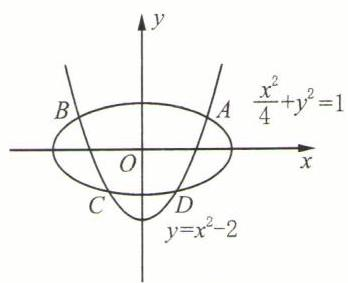
\includegraphics[width=0.2\textwidth]{bodyxb/src/bo_d20cdrf7aajc73bfmvhg_83_1095_1147_348_283_0.jpg}
\end{center}


(第 203 题)

(2)证法一:我们记四个公共点为 $A\left( {{x}_{2},{y}_{2}}\right) ,B\left( {-{x}_{2},{y}_{2}}\right) ,C\left( {-{x}_{1},{y}_{1}}\right) ,D\left( {{x}_{1},{y}_{1}}\right)$ . 设线段 ${BC}$ 的垂直平分线 $l$ 与 $y$ 轴交于点 $M\left( {0,m}\right)$ ,由于 $y$ 轴也是线段 ${AB},{CD}$ 的垂直平分线,故 $\left| {MA}\right|  = \left| {MB}\right|  = \left| {MC}\right|  = \left| {MD}\right|  = r$ ,即四个公共点都在以点 $M$ 为圆心, $r$ 为半径的圆上. 由 $\left| {MB}\right|  = \left| {MC}\right|$ ,得 ${x}_{2}^{2} + {\left( {y}_{2} - m\right) }^{2} = {x}_{1}^{2} + \left( {y}_{1}\right.$  ${\left. -m\right) }^{2}$ ,代入 ${y}_{i} = {x}_{i}^{2} - 2\left( {i = 1,2}\right)$ ,并注意到 ${y}_{1} \neq  {y}_{2}$ ,整理得 $m = \dfrac{1}{2} + \dfrac{1}{2}\left( {{y}_{1} + {y}_{2}}\right)  = \dfrac{1}{2} + \dfrac{1}{2} \cdot  \left( {-\dfrac{1}{4}}\right)  = \dfrac{3}{8}$ ,故 ${r}^{2}$  $= {\left| MB\right| }^{2} = {x}_{2}^{2} + {\left( {y}_{2} - m\right) }^{2} = \dfrac{1}{4}\left( {4{y}_{2}^{2} + {y}_{2}}\right)  + 2 + \dfrac{9}{64} = \dfrac{2}{4} + \dfrac{137}{64} = \dfrac{169}{64}$ ,所求圆为 ${x}^{2} + {\left( y - \dfrac{3}{8}\right) }^{2} = \dfrac{169}{64}$ . 证毕. 证法二: 曲线 $\lambda \left( {{x}^{2} - y - 2}\right)  + \mu \left( {{x}^{2} + 4{y}^{2} - 4}\right)  = 0\left( {\lambda  \cdot  \mu  \neq  0}\right)$ 经过四个公共点,其中 ${x}^{2}$ 的系数为 $\left( {\lambda  + \mu }\right) ,{y}^{2}$ 的系数为 ${4\mu }$ ,令 $\dfrac{\lambda  + \mu }{4\mu } = 1 \Rightarrow  \lambda  = {3\mu }$ ,得 $4{x}^{2} + 4{y}^{2} - {3y} - {10} = 0$ ,故四个公共点同圆. 证毕.

204. (1) 到 $x$ 轴及到点(0,1)距离相等的点在 $\left| y\right|  = \sqrt{{x}^{2} + {\left( y - 1\right) }^{2}}$ 上,即抛物线 ${x}^{2} = 2\left( {y - \dfrac{1}{2}}\right)$ 上. 另外,若(x, y)是两条曲线的一个公共点,那么(-x, y)也一定是一个公共点. 现已知公共点的个数为 2 个,则只有一个 $y \in  D(D =$  $\left( {\dfrac{1}{2}, + \infty }\right)$ )同时满足两条曲线的方程. 方法一: 将抛物线方程代入椭圆,消去 $x$ ,整理得 ${y}^{2} + \left( {4 - {2a}}\right) y + {a}^{2} - 4 =$ 0,记 $f\left( y\right)  = {y}^{2} + \left( {4 + {2a}}\right) y + {a}^{2} - 4$ 方程 $f\left( y\right)  = 0$ 有解,则 $\Delta  = {32} - {16a} \geq  0,\therefore a \leq  2$ . 故 $f\left( y\right)$ 的对称轴在纵坐标轴左侧 (含纵坐标轴),顶点在横坐标轴下方 (或横坐标轴上), $f\left( \dfrac{1}{2}\right)  < 0$ 时能确保 $f\left( y\right)  = 0$ 在 $y > \dfrac{1}{2}$ 时有唯一解. 又 $D \neq  \varnothing$ ,解得, $a$ 的取值范围为 $\dfrac{1}{2} - \sqrt{2} < a < \dfrac{1}{2} + \sqrt{2}$ . 方法二: (参数方程) 将椭圆写成参数方程形式: $\left\{  {\begin{array}{l} x = \cos \theta , \\  y = a + \sqrt{2}\sin \theta , \end{array}\left( {\theta \text{ 为参数, }\theta  \in  \lbrack 0,{2\pi })}\right) }\right.$ . 代入 ${x}^{2} = 2\left( {y - \dfrac{1}{2}}\right)$ ,整理得 $a =  - \dfrac{1}{2}{\left( \sin \theta  + \sqrt{2}\right) }^{2} + 2$ ,当 $\dfrac{1}{2} - \sqrt{2} < a < \dfrac{1}{2}$

$+ \sqrt{2}$ 时,每一个 $a$ 都唯一对应一个 $\sin \theta  \neq   \pm  1$ ,故 $\cos \theta  \neq  0$ ,椭圆和抛物线恰有两个不同的公共点.

(2)方法一:消去 $x$ 得 $4{y}^{2} + y - \left( {m + 4}\right)  = 0$ ,则由 $\left\{  \begin{array}{l} \Delta  > 0, \\  {y}_{1} > m, \\  {y}_{2} > m, \end{array}\right.$ 得 $- \dfrac{65}{16} < m <  - 1$ . 注意 ${y}_{1} > m$ 和 ${y}_{2} > m$ 可以转化为 $\dfrac{-1 - \sqrt{\Delta }}{8} > m$ 来求解. 方法二: (参数方程) 将椭圆写成参数方程形式 $\left\{  {\begin{array}{l} x = 2\cos \theta , \\  y = \sin \theta , \end{array}\left( {\theta \text{ 为参数, }\theta  \in  \lbrack 0,{2\pi })}\right) }\right.$ . 代入 ${x}^{2} = y - m$ ,整理得 $m = 4{\left( \sin \theta  + \dfrac{1}{8}\right) }^{2} - \dfrac{65}{16}$ ,如图,当 $- \dfrac{65}{16} < m <  - 1$ 时,每一个 $m$ 都对应两个不同的 $\sin \theta  \neq   \pm  1$ ,故椭圆和抛物线恰有四个不同的公共点.

\begin{center}
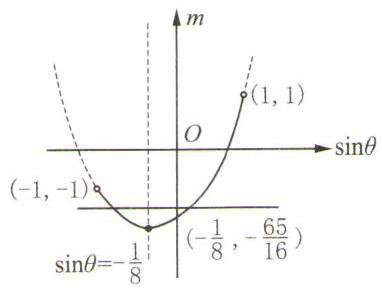
\includegraphics[width=0.3\textwidth]{bodyxb/src/bo_d20cdrf7aajc73bfmvhg_84_1144_178_382_291_0.jpg}
\end{center}


(第 204 题)

205. (1) 可得 $A\left( {1,3}\right) ,B\left( {-4, - {12}}\right)$ ,设抛物线上点 $P\left( {{x}_{0},4 - {x}_{0}^{2}}\right)$ 到 ${AB}$ 的距离为 $d$ ,则 $d = \dfrac{\left| 3{x}_{0} - 4 + {x}_{0}^{2}\right| }{\sqrt{10}}$ . 由 $- 4 \leq  {x}_{0} \leq  1$ , 得 $d = \dfrac{-{\left( {x}_{0} + \dfrac{3}{2}\right) }^{2} + \dfrac{25}{4}}{\sqrt{10}}$ . $\therefore$ 当 $P\left( {-\dfrac{3}{2},\dfrac{7}{4}}\right)$ 时, ${d}_{\max } = \dfrac{25}{4\sqrt{10}}$ . (2)由 $\left\{  \begin{array}{l} y = {3x} + b, \\  y = 4 - {x}^{2} \end{array}\right.$ 消去 $y$ 得 ${x}^{2} + {3x} + b - 4 = 0$ ,于是可得 ${CD}$ 中点 $Q$ 的横坐标 ${x}_{Q} =  - \dfrac{3}{2}$ . 注: 关于这一问,我们证明一个更一般的情形:抛物线平行弦的中点在同一直线上. 证明: 不妨设抛物线为 ${x}^{2} = {2py}\left( {p > 0}\right)$ ,此时平行弦所在的直线斜率一定存在,设直线方程为 $y = {kx} + b$ ,代入抛物线方程,消去 $y$ ,整理得 ${x}^{2} - {2pkx} - {2pb} = 0,\Delta  = {4p}\left( {p{k}^{2} + }\right.$  ${2b})$ ,当 $b >  - \dfrac{p{k}^{2}}{2}$ 时, $\Delta  > 0$ . 此时, $\dfrac{{x}_{1} + {x}_{2}}{2} = {pk}$ ,故平行弦的中点都在定直线 $x = {pk}$ 上. 证毕.

206. (1) 方法一: 设 $A\left( {{x}_{1},{y}_{1}}\right) ,B\left( {{x}_{2},{y}_{2}}\right)$ ,则由 ${AF}\bot {BF}$ ,得 $\dfrac{{y}_{1}}{{x}_{1} - 2} \cdot  \dfrac{{y}_{2}}{{x}_{2} - 2} =  - 1$ ,

即 ${y}_{1}{y}_{2} =  - \left\lbrack  {{x}_{1}{x}_{2} - 2\left( {{x}_{1} + {x}_{2}}\right)  + 4}\right\rbrack$ ,再将 $l : y = {kx}\left( {k \neq  0}\right)$ 代入曲线方程得 ${k}^{2}{x}^{2} - {4x} + 4 = 0$ ,

$\therefore \left\{  \begin{array}{l} {x}_{1} + {x}_{2} = \dfrac{4}{{k}^{2}}, \\  {x}_{1}{x}_{2} = \dfrac{4}{{k}^{2}}. \end{array}\right.$ 又可求得 ${y}_{1}{y}_{2} = 4$ ,由此得 $k =  \pm  \dfrac{\sqrt{2}}{2},\therefore$ 直线 $l$ 的方程为 $y =  \pm  \dfrac{\sqrt{2}}{2}x$ ;

注: ${y}_{1}^{2}{y}_{2}^{2} = {16}\left( {{x}_{1} - 1}\right) \left( {{x}_{2} - 1}\right)  = {16}\left( {{x}_{1}{x}_{2} - {x}_{1} - {x}_{2} + 1}\right)  = {16}$ ,又 ${y}_{1}{y}_{2} > 0,\;\therefore \;{y}_{1}{y}_{2} = 4$ . 方法二: 设 $A\left( {{x}_{1},{y}_{1}}\right)$ , $B\left( {{x}_{2},{y}_{2}}\right) \left( {{x}_{1} > 1,{x}_{2} > 1}\right)$ ,线段 ${AB}$ 的中点为 $M\left( {{x}_{M},{y}_{M}}\right)$ ,线段 ${AB}$ 所在直线斜率存在,设为 $y = {kx}\left( {k \neq  0}\right)$ . 注意到 $y$ 轴恰好是抛物线的准线,故 $\left| {FA}\right|  = {x}_{1},\left| {FB}\right|  = {x}_{2}.\bigtriangleup {AFB}$ 中, $\angle {AFB} = {90}^{ \circ  }$ ,运用勾股定理: ${x}_{1}^{2} + {x}_{2}^{2} =$  ${\left| AB\right| }^{2} = {\left( {x}_{2} - {x}_{1}\right) }^{2} + {\left( {y}_{2} - {y}_{1}\right) }^{2}$ ,整理得 $2{x}_{1}{x}_{2} = {\left( {y}_{1} - {y}_{2}\right) }^{2}$ . 运用点差法, $\left( {{y}_{1} + {y}_{2}}\right) \left( {{y}_{1} - {y}_{2}}\right)  = 4\left( {{x}_{1} - {x}_{2}}\right)$ ,其中 ${y}_{1} + {y}_{2} = 2{y}_{M} = {2k}{x}_{M} = k\left( {{x}_{1} + {x}_{2}}\right) ,\;\therefore \;2{x}_{1}{x}_{2} = {\left( {y}_{1} - {y}_{2}\right) }^{2} = {\left\lbrack  \dfrac{4\left( {{x}_{1} - {x}_{2}}\right) }{k\left( {{x}_{1} + {x}_{2}}\right) }\right\rbrack  }^{2}$ (*). 将 $y = {kx}$ 代入 ${y}^{2} = 4(x -$ 1),消去 $y$ ,整理得 ${k}^{2}{x}^{2} - {4x} + 4 = 0\left( {\Delta  = {16}\left( {1 - {k}^{2}}\right) }\right)$ ,故 ${x}_{1} + {x}_{2} = \dfrac{4}{{k}^{2}},{x}_{1}{x}_{2} = \dfrac{4}{{k}^{2}},{\left( {x}_{1} - {x}_{2}\right) }^{2} = {\left( {x}_{1} + {x}_{2}\right) }^{2} - 4{x}_{1}{x}_{2}$  $= \dfrac{16}{{k}^{4}} - \dfrac{16}{{k}^{2}}$ ,代入 $\left( {}^{ * }\right)$ 式,整理得 $\dfrac{8}{{k}^{2}} = \dfrac{16}{{k}^{2}} - {16}$ ,故 $k =  \pm  \dfrac{\sqrt{2}}{2}\left( {\Delta  > 0}\right)$ ,故直线 $l : y =  \pm  \dfrac{\sqrt{2}}{2}x$ .

(2) $\left| {AB}\right|  = \sqrt{1 + {k}^{2}} \cdot  \left| {{x}_{1} - {x}_{2}}\right|  = \dfrac{4}{{k}^{2}}\sqrt{1 - {k}^{4}} = 4\sqrt{3}$ .

207. (1) 记重心坐标为 $G\left( {x,y}\right)$ ,椭圆中心为 $M\left( {2, - 1}\right) .A,B$ 两点在抛物线下方,故 $A,B,C$ 三点总能形成三角形. 由三角形重心的性质, $\vv{GC} =  - \dfrac{2}{3}\vv{CM}$ ,使用定比分点公式,求得点 $C\left( {{3x} - 4,{3y} + 2}\right)$ 在抛物线上,故有 ${3y} + 2 = {\left( 3x - 4\right) }^{2}$ , 整理得 ${\left( x - \dfrac{4}{3}\right) }^{2} = \dfrac{1}{3}\left( {y + \dfrac{2}{3}}\right)$ .

(2)记已知圆的圆心分别为 $A\left( {0,0}\right) ,B\left( {r,0}\right)$ ；半径分别为 ${r}_{1} = {2r},{r}_{2} = r$ ,动圆半径为 $R$ . 由题意: $\left| {MA}\right|  = \left| {R - {r}_{1}}\right|$ , $\left| {MB}\right|  = R + {r}_{2}$ . ① 若 $\left| {MA}\right|  = \left| {R - {r}_{1}}\right|  = R - {r}_{1}$ ,则有 $\left| {MB}\right|  - \left| {MA}\right|  = {r}_{1} + {r}_{2} = {3r}$ ,另一方面, $\left| {MB}\right|  -$  $\left| {MA}\right|  \leq  \left| {AB}\right|  = r$ ,故这样的点 $M$ 不存在. ②若 $\left| {MA}\right|  = \left| {R - {r}_{1}}\right|  = {r}_{1} - R$ ,则有 $\left| {MA}\right|  + \left| {MB}\right|  = {r}_{1} + {r}_{2} = {3r}$ ,

点 $M$ 在以线段 ${AB}$ 的中点 $\left( {\dfrac{r}{2},0}\right)$ 为中心,焦点在 $x$ 轴上的椭圆上,且有 ${2a} = {3r},{2c} = \left| {AB}\right|  = r,\therefore {b}^{2} = {a}^{2} - {c}^{2} =$  $2{r}^{2}$ ,故所求轨迹方程为 $\dfrac{4{\left( x - \dfrac{r}{2}\right) }^{2}}{9{r}^{2}} + \dfrac{{y}^{2}}{2{r}^{2}} = 1\left( {x \neq  {2r}}\right)$ .

(3)记已知圆的圆心分别为 $A\left( {0,0}\right) ,B\left( {4,0}\right)$ ；半径分别为 ${r}_{1} = 1,{r}_{2} = 3$ ,动圆半径为 $R.\left| {MA}\right|  = \left| {R - {r}_{1}}\right| ,\left| {MB}\right|  = R -$  ${r}_{2}$ . 由题意 $R > 3$ ,此时 $\left| {MA}\right|  - \left| {MB}\right|  = \left( {R - {r}_{1}}\right)  - \left( {R - {r}_{2}}\right)  = 2$ ,故点 $M$ 在以线段 ${AB}$ 的中点(2,0)为中心,焦点在 $x$ 轴上的双曲线 (右支) 上,且有 ${2a} = 2,{2c} = \left| {AB}\right|  = 4,\therefore {b}^{2} = {c}^{2} - {a}^{2} = 3$ ,故所求轨迹方程为 ${\left( x - 2\right) }^{2} - \dfrac{{y}^{2}}{3}$  $= 1\left( {x \geq  3}\right)$ .

(4) 记已知圆的圆心为 $A\left( {-2,0}\right)$ ; 半径为 $r = 2$ ,动圆圆心为 $M\left( {x,y}\right)$ ,半径为 $R$ . 由题意得 $\left\{  \begin{array}{l} \left| {MA}\right|  = \sqrt{{\left( x + 2\right) }^{2} + {y}^{2}} = R + r = R + 2, \\  \left| {x - 2}\right|  = R. \end{array}\right.$ ①若 $x \geq  2$ ,整理可得 ${y}^{2} =  - 4\left( {x + 1}\right)$ ,不存在这样的点 $M$ . ②若 $x < 2$ , 整理可得 ${y}^{2} =  - {12}\left( {x - 1}\right)$ ,此即动圆圆心 $M$ 的轨迹方程,轨迹是顶点为(1,0),开口向左的抛物线.

(5)记 $A\left( {-5,{12}}\right) ,B\left( {9,{12}}\right)$ . 由椭圆的性质, $\left| {AO}\right|  + \left| {AF}\right|  = \left| {BO}\right|  + \left| {BF}\right|$ 均为长轴长,其中 $\left| {AO}\right|  = {13},\left| {BO}\right|  =$  ${15},\therefore \left| {AF}\right|  - \left| {BF}\right|  = 2$ . 因此,点 $F$ 在以线段 ${AB}$ 的中点(2,12)为中心,焦点连线平行于 $x$ 轴的双曲线 (右支)上,且 ${2a} = 2,{2c} = \left| {AB}\right|  = {14},\therefore {b}^{2} = {c}^{2} - {a}^{2} = {48}$ ,故所求轨迹方程为 ${\left( x - 2\right) }^{2} - \dfrac{{\left( y - {12}\right) }^{2}}{48} = 1$ (右支).

208. 不妨设点 $C$ 在点 $B$ 上方,则设 $B\left( {0,b}\right) ,C\left( {0,b + {2a}}\right) \left( {b \geq  0}\right)$ ,圆心 $M$ 在线段 ${BC}$ 的垂直平分线上,故可设为 $M\left( {m,a + b}\right)$ . 由 $\left| {MB}\right|  = \left| {MA}\right|$ ,可得 $\sqrt{{m}^{2} + {a}^{2}} = \sqrt{{\left( m - 3\right) }^{2} + {\left( a + b\right) }^{2}}$ , 解得 $m = \dfrac{{b}^{2} + {2ab} + 9}{6}$ . 故 $\left\{  \begin{array}{l} {x}_{M} = \dfrac{{b}^{2} + {2ab} + 9}{6}, \\  {y}_{M} = a + b, \end{array}\right.$ ( $b$ 是参数, $b \geq  0$ ),将 $b = {y}_{M} - a$ 代入 ${x}_{M}$ ,整理得 ${y}^{2} = 6\left( {x + \dfrac{{a}^{2} - 9}{6}}\right) \left( {y \geq  a}\right)$ ,是以 $\left( {\dfrac{9 - {a}^{2}}{6},0}\right)$ 为顶点, $x$ 轴为对称轴,开口向右的抛物线上满足 $y \geq  a$ 的部分 (如图).

\begin{center}
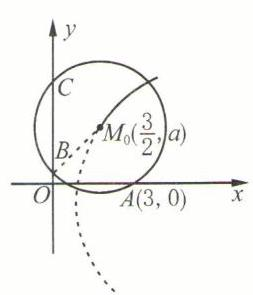
\includegraphics[width=0.2\textwidth]{bodyxb/src/bo_d20cdrf7aajc73bfmvhg_85_1161_649_253_295_0.jpg}
\end{center}


(第 208 题)

209. (1) 设 $P\left( {x,y}\right) \left( {y > 0}\right)$ ,则焦点 $F\left( {x,{2y}}\right)$ ,于是由 ${\left( x - 0\right) }^{2} + {\left( 2y - 2\right) }^{2} = 4$ ,得轨迹方程为 $\dfrac{{x}^{2}}{4}$  $+ {\left( y - 1\right) }^{2} = 1\left( {y > 0}\right)$ .

\begin{center}
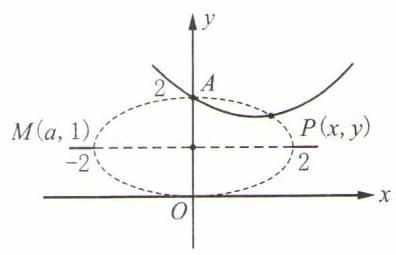
\includegraphics[width=0.3\textwidth]{bodyxb/src/bo_d20cdrf7aajc73bfmvhg_85_1044_1019_396_255_0.jpg}
\end{center}


(第 209 题)

(2)方法一:设过 $M\left( {a,1}\right)$ 的直线为 $y - 1 = k\left( {x - a}\right)$ ,与椭圆 $C$ 联立消 $y$ ,得 $\left( {4{k}^{2} + }\right.$ 1) ${x}^{2} - 8{k}^{2}{ax} + 4{k}^{2}{a}^{2} - 4 = 0$ ,其 $\Delta  = {16}\left\lbrack  {{k}^{2}\left( {4 - {a}^{2}}\right)  + 1}\right\rbrack$ ,于是 “过 $M$ 存在一对同时与 $C$ 有公共点且互相垂直的直线”的充要条件是 “关于 $k$ 的不等式组 $\left\{  \begin{array}{l} {k}^{2}\left( {4 - {a}^{2}}\right)  + 1 \geq  0, \\  \dfrac{1}{{k}^{2}}\left( {4 - {a}^{2}}\right)  + 1 \geq  0 \end{array}\right.$ 有解”,由此得 $\left\{  \begin{array}{l} {k}^{2} \leq  \dfrac{1}{{a}^{2} - 4}, \\  {k}^{2} \geq  {a}^{2} - 4, \end{array}\right.$ 求得 $2 < \left| a\right|  \leq  \sqrt{5}$ . 方法二: 作坐标平移 $\left\{  \begin{array}{l} {x}^{\prime } = x, \\  {y}^{\prime } = y - 1, \end{array}\right.$ 在 ${x}^{\prime }{O}^{\prime }{y}^{\prime }$ 中,曲线 $C$ 为 ${C}^{\prime } : \dfrac{{x}^{\prime 2}}{4} + {y}^{\prime 2} = 1\left( {{y}^{\prime } >  - 1}\right)$ ,点 ${M}^{\prime }\left( {a,0}\right)$ 不在线段 ${y}^{\prime } = 0\left( {-2 \leq  {x}^{\prime } \leq  2}\right.$ ,即椭圆 ${C}^{\prime }$ 的长轴) 上. 过点 ${M}^{\prime }\left( {a,0}\right)$ 向椭圆引切线,切点为 ${Q}^{\prime }\left( {\dfrac{4}{a},\sqrt{1 - \dfrac{4}{{a}^{2}}}}\right) ,{R}^{\prime }\left( {\dfrac{4}{a}, - \sqrt{1 - \dfrac{4}{{a}^{2}}}}\right)$ ,故 $\angle {Q}^{\prime }{M}^{\prime }{R}^{\prime } = 2\arctan \dfrac{1}{\sqrt{{a}^{2} - 4}}$ ,可见 $\left| a\right|  > 2$ 时, $\angle {Q}^{\prime }{M}^{\prime }{R}^{\prime }$ 随着 $\left| a\right|$ 的增大而减小. 由题意, $\angle {Q}^{\prime }{M}^{\prime }{R}^{\prime } \geq  \dfrac{\pi }{2}$ ,故 $\dfrac{1}{\sqrt{{a}^{2} - 4}} \geq  1,\;\therefore \;2 < \left| a\right|  \leq  \sqrt{5}$ .

210. (1) 由题意, $\left\{  \begin{array}{l} 2 \cdot  {2a} = {2b} + {2c}, \\  {c}^{2} = {a}^{2} + {b}^{2}, \end{array}\right.$ 解得 $\left\{  \begin{array}{l} a = {4k}, \\  b = {3k},\left( {k > 0,k \in  \mathbf{R}}\right) \text{ . 由双曲线的第二定义,点 }M\text{ 到右焦点 }P\left( {x,y}\right) \text{ 的距离和点 } \\  c = {5k} \end{array}\right.$  $M$ 到右准线的距离之比为 $e = \dfrac{c}{a} = \dfrac{5}{4}$ ,即 $\dfrac{\sqrt{{\left( x - 2\right) }^{2} + {\left( y - 3\right) }^{2}}}{2} = \dfrac{5}{4}$ ,整理得点 $P$ 的轨迹为 ${\left( x - 2\right) }^{2} + {\left( y - 3\right) }^{2}$  $= \dfrac{25}{4}$ ( $x > 0$ ,因为双曲线的右焦点在右准线的右侧).

(2)由于点 $M\left( {1,0}\right)$ 在准线 $x + 2 = 0$ 右侧,故该准线是左准线. 由 $e = \dfrac{c}{a} = \dfrac{1}{2}$ ,设 $\left\{  {\begin{array}{l} a = {2k}, \\  b = \sqrt{3}k, \\  c = k \end{array}\left( {k > 0,k \in  \mathbf{R}}\right) }\right.$ . 由椭圆的第二定义,点 $M$ 到左焦点 $F\left( {x,y}\right)$ 的距离和点 $M$ 到左准线的距离之比为 $e = \dfrac{1}{2}$ ,即 $\dfrac{\sqrt{{\left( x - 1\right) }^{2} + {y}^{2}}}{3} = \dfrac{1}{2}$ ,整理得左焦点 $F$ 的轨迹为 $C : {\left( x - 1\right) }^{2} + {y}^{2} = \dfrac{9}{4}$ ,是以点 $M$ 为圆心,半径为 $\dfrac{3}{2}$ 的圆. 左焦点到左准线的距离为 $p = \dfrac{{b}^{2}}{c} = {3k} = \dfrac{3}{2}a$ , 故欲使得长轴长最大. 需使得左焦点到左准线的距离最大,轨迹 $C$ 上到 $x + 2 = 0$ 的距离最大的点是 $F\left( {\dfrac{5}{2},0}\right)$ ,此

时 $p = \dfrac{3}{2}a = \dfrac{9}{2}$ ,故求得 $\left\{  \begin{array}{l} a = 3, \\  b = \dfrac{3\sqrt{3}}{2}, \\  c = \dfrac{3}{2}, \end{array}\right.$ 椭圆中心为 $\left( {\dfrac{5}{2} + c,0}\right)$ ,即 (4,0) ,此时椭圆方程为 $\dfrac{{\left( x - 4\right) }^{2}}{9} + \dfrac{4{y}^{2}}{27} = 1$ .

211. (1) 设中心 ${O}^{\prime }\left( {x,y}\right)$ ,右顶点 $P\left( {{x}_{1},{y}_{1}}\right)$ ,则将 $\left\{  \begin{array}{l} {x}_{1} = x + 2, \\  {y}_{1} = y, \end{array}\right.$ 代入 ${y}_{1}^{2} = {x}_{1} - 1 \geq  0$ ,中心 ${O}^{\prime }$ 的轨迹方程是 ${y}^{2} = x + 1( - 1 \leq$  $x < 0)$ ,它表示顶点在(-1,0),焦点为 $\left( {-\dfrac{3}{4},0}\right)$ 的抛物线的一部分 $\left( {-1 \leq  x < 0}\right)$ .

(2)可设双曲线为 $\dfrac{{\left( x - {x}_{0}\right) }^{2}}{4} - \dfrac{{\left( y - {y}_{0}\right) }^{2}}{{b}^{2}} = 1$ ,则 ${x}_{0} =  - \dfrac{4}{c}$ ,代入 ${y}_{0}^{2} = {x}_{0} + 1$ ,得 ${y}_{0}^{2} = 1 - \dfrac{4}{c} \geq  0$ ,于是 ${c}_{\text{ 最小值 }} = 4$ , ${e}_{\text{ 最小值 }} =$ 2,双曲线方程为 $\dfrac{{\left( x + 1\right) }^{2}}{4} - \dfrac{{y}^{2}}{12} = 1$ . 注:①双曲线中心 $\left( {{x}_{0},{y}_{0}}\right)$ 到右准线 $x = 0$ 的距离是 $- {x}_{0} = \dfrac{{a}^{2}}{c} = \dfrac{4}{c}$ ,故有 ${x}_{0} =$  $- \dfrac{4}{c}$ . ②也可通过 $- 1 \leq  {x}_{0} < 0$ ,直接得到 $c \geq  4$ ,进而求解.

212. 方法一:由 $\dfrac{\sqrt{6}}{3} < e < 1$ ,得 $0 < \alpha  < \dfrac{\pi }{6}$ . 将 $B\left( {\sin \alpha ,\sin \alpha }\right)$ 代入抛物线 ${y}^{2} =  - 4\left( {m - 1}\right) \left( {x - m}\right)$ ,

得 ${\sin }^{2}\alpha  + 4\left( {m - 1}\right) \sin \alpha  - {4m}\left( {m - 1}\right)  = 0$ . 设 $f\left( t\right)  = {t}^{2} + 4\left( {m - 1}\right) t - {4m}\left( {m - 1}\right)$ . 由 $m > 1$ ,得 $f\left( 0\right)  < 0$ .

又 $\because f\left( t\right)$ 图像顶点的横坐标小于 0, $\therefore f\left( \dfrac{1}{2}\right)  > 0$ ,由此可得 $1 < m < \dfrac{3 + \sqrt{2}}{4}$ .

方法二: 在得到 $\alpha  \in  \left( {0,\dfrac{\pi }{6}}\right)$ ,及 $B\left( {\sin \alpha ,\sin \alpha }\right)$ 后,由抛物线的性质,点 $B$ 到抛物线准线的距离等于 $\left| {AB}\right|  =$  $\sqrt{{\left( 1 - \sin \alpha \right) }^{2} + {\sin }^{2}\alpha }$ ,故准线方程为 $x = \left| {AB}\right|  + {x}_{B}$ ,从而 $m = \dfrac{\left| {AB}\right|  + {x}_{B} + {x}_{A}}{2} = \dfrac{1 + \sin \alpha  + \sqrt{2{\sin }^{2}\alpha  - 2\sin \alpha  + 1}}{2}$ . 令 $u$  $= \sin \alpha  - \dfrac{1}{2} \in  \left( {-\dfrac{1}{2},0}\right)$ ,则 $m = \dfrac{1}{4}\left( {3 + {2u} + \sqrt{2}\sqrt{4{u}^{2} + 1}}\right)$ ; 再令 ${2u} = \tan \theta  \in  \left( {-1,0}\right)$ (即 $\theta  \in  \left( {-\dfrac{\pi }{4},0}\right)$ ),得 $m =$  $\dfrac{1}{4}\left( {3 + \tan \theta  + \dfrac{\sqrt{2}}{\cos \theta }}\right)  = \dfrac{1}{4}\left( {3 + \dfrac{\sin \theta  - \left( {-\sqrt{2}}\right) }{\cos \theta  - 0}}\right)$ ,将 $f\left( \theta \right)  = \dfrac{\sin \theta  - \left( {-\sqrt{2}}\right) }{\cos \theta  - 0}$ 视作单位圆上的点 $\left( {\cos \theta ,\sin \theta }\right) (\theta  \in$  $\left( {-\dfrac{\pi }{4},0}\right)$ ) 和定点 $\left( {0, - \sqrt{2}}\right)$ 连线的斜率,不难看出 $f\left( \theta \right)$ 在 $\theta  \in  \left( {-\dfrac{\pi }{4},0}\right)$ 上单调递增,故 $m$ 的值域是 $\left( {\dfrac{1}{4}\left( {3 + f\left( \dfrac{\pi }{4}\right) }\right) ,\dfrac{1}{4}\left( {3 + f\left( 0\right) }\right) }\right)$ ,即 $1 < m < \dfrac{3 + \sqrt{2}}{4}.$

213. 方法一:渐近线为 $\dfrac{\sqrt{{a}^{2} - 1}}{a}x \pm  y = 0$ ,故由 $\dfrac{\sqrt{3}}{2} \leq  \dfrac{\sqrt{{a}^{2} - 1}}{a} \leq  \dfrac{2\sqrt{2}}{3}$ ,得 $2 \leq  a \leq  3$ ,然后求得 $B\left( {a,a}\right) ,A\left( {0,1}\right)$ . 设 $P\left( {0,m}\right) (m$  $> 1)$ ,则抛物线方程为 ${x}^{2} =  - 4\left( {m - 1}\right) \left( {y - m}\right)$ . 将(a, a)代入,可得 $m = \dfrac{a + 1}{2} + \dfrac{1}{2}\sqrt{2{\left( a - \dfrac{1}{2}\right) }^{2} + \dfrac{1}{2}}$ . 又 $\dfrac{a + 1}{2}$ 及 $\dfrac{1}{2}\sqrt{2{\left( a - \dfrac{1}{2}\right) }^{2} + \dfrac{1}{2}}$ 在 $2 \leq  a \leq  3$ 上都是严格递增, $\therefore {m}_{\text{ 最小值 }} = \dfrac{3 + \sqrt{5}}{2},{m}_{\text{ 最大值 }} = \dfrac{4 + \sqrt{13}}{2}$ . $\therefore$ 抛物线顶点 $P$ 的纵坐标的取值范围是 $\dfrac{3 + \sqrt{5}}{2} \leq  y \leq  \dfrac{4 + \sqrt{13}}{2}$ .

方法二:在得到 $A\left( {0,1}\right)$ 和 $B\left( {a,a}\right)$ 后,无需解二次方程,便可直接写出点 $P\left( {0,m}\right)$ 的坐标:根据抛物线的性质,点 $B$ 到抛物线准线的距离等于 $\left| {AB}\right|$ ,故抛物线的准线为 $y = \left| {AB}\right|  + {y}_{B}$ . 点 $P$ 的横坐标是 $\left| {AB}\right|  + {y}_{B}$ 与点 $A$ 横坐标的平均值,即 $m = \dfrac{\left| {AB}\right|  + {y}_{B} + {y}_{A}}{2} = \dfrac{a + 1}{2} + \dfrac{1}{2}\sqrt{{a}^{2} + {\left( a - 1\right) }^{2}} = \dfrac{a + 1}{2} + \dfrac{1}{2}\sqrt{2{\left( a - \dfrac{1}{2}\right) }^{2} + \dfrac{1}{2}}$ ,余下略.

214. 方法一: (数形结合) 如图, ${y}_{1} = \sqrt{1 - {x}^{2}}$ 代表的是单位圆 ${x}^{2} + {y}^{2} = 1$ 在 $x$ 轴以上的部分 (包含两个端点 $B\left( {-1,0}\right)$ 和 $C\left( {1,0}\right)$ ); ${y}_{2} = {mx} + 1$ 是过定点 $A\left( {0,1}\right)$ ,斜率为 $m$ 的直线. 显然,不论 $m$ 取何值,均有 $x = 1$ 这个解,根据题意,半圆与直线的公共点除点 $A$ 以外无其他公共点. 讨论: ① $m = 0$ ,即图中 ${l}_{1}$ ,此时直线与半圆相切,符合题意. ② $m$  $> 0$ ,即图中 ${l}_{2}$ 的位置,当 $m > {k}_{AB} = 1$ 时,直线与半圆只有一个公共点. ③ $m < 0$ ,即图中 ${l}_{3}$ 的位置,当 $m < {k}_{AC} =  - 1$ 时,直线与半圆只有一个公共点. 综上, $m <  - 1$ 或 $m =$ 0 或 $m > 1$ . 方法二: (解方程) 将 $\sqrt{1 - {x}^{2}} = {mx} + 1$ 两边平方,整理得 $\left( {{m}^{2} + 1}\right) {x}^{2} +$

\begin{center}
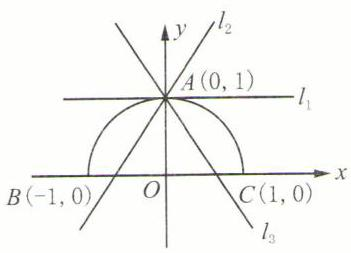
\includegraphics[width=0.3\textwidth]{bodyxb/src/bo_d20cdrf7aajc73bfmvhg_86_1186_1804_351_253_0.jpg}
\end{center}


(第 214 题)

${2mx} = 0,\therefore {x}_{1} = 0,{x}_{2} =  - \dfrac{2m}{{m}^{2} + 1}$ . 显然, ${x}_{1} = 0$ 是原方程的一个解,为使得 ${x}_{1} = 0$ 是唯一解,有以下两种情形: $\text{ ① }{x}_{2}$  $= {x}_{1} = 0$ ,此时 $m = 0$ ; ② 解 ${x}_{2} =  - \dfrac{2m}{{m}^{2} + 1}$ 不符合,即 $m{x}_{2} + 1 < 0 \Leftrightarrow  {m}^{2} > 1,\therefore m <  - 1$ 或 $m > 1$ . 综上, $m <  - 1$ 或 $m =$ 0 或 $m > 1$ . 方法三:(三角函数)令 $x = \sin \theta \left( {\theta  \in  D,D = \left\lbrack  {-\dfrac{\pi }{2},\dfrac{\pi }{2}}\right\rbrack  }\right.$ ),由题意,三角方程 $\cos \theta  = m\sin \theta  + 1$ 在 $\theta  \in  D$ 时有且只有一个解. 由于 $\theta  = 0$ 满足该方程,故 $\theta$ 在 $D$ 上没有非零解,此时 $m = \dfrac{\cos \theta  - 1}{\sin \theta } =  - \tan \dfrac{\theta }{2}$ ,当 $\theta  \in  D$ 且 $\theta  \neq  0$ 时的值域是 $\left\lbrack  {-1,0)\bigcup (0,1}\right\rbrack$ ,因此 $m <  - 1$ 或 $m = 0$ 或 $m > 1$ 时,原方程有且只有一个实数解.

215. (1) 方法一:记圆心 $C\left( {4,3}\right) ,A\left( {6, - 2}\right) ,B\left( {-6, - 3}\right)$ ,则 ${u}_{\text{ 最大值 }} = {\left( \left| AC\right|  + 2\right) }^{2} = {\left( 2 + \sqrt{29}\right) }^{2} = {33} + 4\sqrt{29},{u}_{\text{ 最小值 }} =$  ${\left( \sqrt{29} - 2\right) }^{2} = {33} - 4\sqrt{29}$ ,关于 $v$ ,等式改写为 ${vx} - y + {6v} - 3 = 0$ . 圆心 $C$ 到该直线的距离不大于半径故 $\dfrac{\left| 4v - 3 + 6v - 3\right| }{\sqrt{{v}^{2} + 1}} \leq  2$ . 得 $\dfrac{{15} - \sqrt{33}}{24} \leq  v \leq  \dfrac{{15} + \sqrt{33}}{24}$ ,得 ${v}_{\max } = \dfrac{{15} + \sqrt{33}}{24},{v}_{\min } = \dfrac{{15} - \sqrt{33}}{24}$ . 方法二: (参数方程) 关于 $u$ 的取值范围,还可以使用参数方程求解. 令 $\left\{  {\begin{array}{l} x = 4 + 2\cos \theta , \\  y = 3 + 2\sin \theta  \end{array}\left( \theta \right. }\right.$ 定参数, $\left. {\theta  \in  \lbrack 0,{2\pi })}\right)$ ,则 $u = {\left( 2\cos \theta  - 2\right) }^{2} + {\left( 2\sin \theta  + 5\right) }^{2}$  $= {33} + 4\sqrt{29}\sin \left( {\theta  - \varphi }\right) \left( {\tan \varphi  = \dfrac{2}{5}}\right)$ ,故 ${u}_{\max } = {33} + 4\sqrt{29},{u}_{\min } = {33} - 4\sqrt{29}$ .

(2)令 ${\log }_{a}x = m,{\log }_{a}y = n$ ,则由题意,(m, n)满足 ${\left( m - 1\right) }^{2} + {\left( n - 1\right) }^{2} = 4$ ,即在圆心为 $C\left( {1,1}\right)$ ,半径为 2 的圆上. ${\log }_{a}\left( {xy}\right)  = m + n$ .

\begin{center}
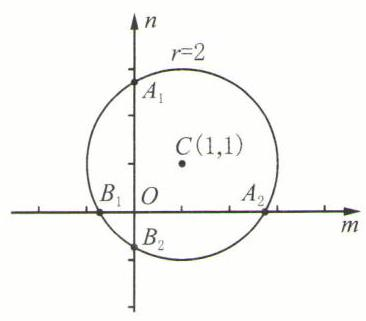
\includegraphics[width=0.3\textwidth]{bodyxb/src/bo_d20cdrf7aajc73bfmvhg_87_1067_788_366_321_0.jpg}
\end{center}


[第 215(2)题]

方法一: (数形结合) 令 $L = m + n$ ,则 $n =  - m + L$ ,是斜率为 -1,截距为 $L$ 的直线. 如图,圆 $C$ 与 $x$ 轴正、负半轴分别交于点 ${A}_{2}\left( {1 + \sqrt{3},0}\right) ,{B}_{1}\left( {1 - \sqrt{3},0}\right)$ ,与 $y$ 轴正、负半轴分别交于点 ${A}_{1}\left( {0,1 + \sqrt{3}}\right) ,{B}_{2}\left( {0,1 - \sqrt{3}}\right)$ ,且 ${k}_{{A}_{1}{A}_{2}} = {k}_{{B}_{1}{B}_{2}} =  - 1$ . 直线 $n =  - m + L$ 与圆 $C$ 相切时,有 $\dfrac{\left| 1 + 1 - L\right| }{\sqrt{2}} = 2$ ,此时 $L = 2 \pm  2\sqrt{2}$ . ①当 $a >$ 1 时, $m \geq  0,n \geq  0$ ,点(m, n)位于圆 $C$ 在第一象限的圆弧部分 (包含两个端点), 直线 $n =  - m + L$ 自直线 ${A}_{1}{A}_{2}$ 开始,向上平移直至与圆 $C$ 相切,故 $1 + \sqrt{3} \leq$  ${\log }_{a}\left( {xy}\right)  \leq  2 + 2\sqrt{2}$ . ②当 $0 < a < 1$ 时, $m \leq  0,n \leq  0$ ,点(m, n)位于圆 $C$ 在第三象限的圆弧部分 (包含两个端点),直线 $n =  - m + L$ 自直线 ${B}_{1}{B}_{2}$ 开始,向下平移直至与圆 $C$ 相切,故 $2 - 2\sqrt{2} \leq  {\log }_{a}\left( {xy}\right)  \leq  1 - \sqrt{3}$ .

方法二: (参数方程) 令 $\left\{  \begin{array}{l} m = 1 + 2\cos \theta , \\  n = 1 + 2\sin \theta  \end{array}\right.$ ( $\theta$ 是参数, $\theta  \in  \lbrack  - \pi ,\pi )$ ), ${\log }_{a}\left( {xy}\right)  = m + n = 2\left( {\sin \theta  + \cos \theta }\right)  + 2 =$  $2\sqrt{2}\sin \left( {\theta  + \dfrac{\pi }{4}}\right)  + 2$ . ①当 $a > 1$ 时, $\left\{  \begin{array}{l} m = 1 + 2\cos \theta  \geq  0, \\  n = 1 + 2\sin \theta  \geq  0, \end{array}\right.$ 解得 $\theta  \in  \left\lbrack  {-\dfrac{\pi }{6},\dfrac{2\pi }{3}}\right\rbrack$ ,故 $\theta  + \dfrac{\pi }{4} \in  \left\lbrack  {\dfrac{\pi }{12},\dfrac{11\pi }{12}}\right\rbrack  ,{\log }_{a}\left( {xy}\right)$ 在 $\theta  + \dfrac{\pi }{4}$  $= \dfrac{\pi }{12}$ 或 $\theta  + \dfrac{\pi }{4} = \dfrac{11\pi }{12}$ 时取得最小值,在 $\theta  + \dfrac{\pi }{4} = \dfrac{\pi }{2}$ 时取得最大值,故 $1 + \sqrt{3} \leq  {\log }_{a}\left( {xy}\right)  \leq  2 + 2\sqrt{2}$ .

②当 $0 < a < 1$ 时, $\left\{  \begin{array}{l} m = 1 + 2\cos \theta  \leq  0, \\  n = 1 + 2\sin \theta  \leq  0, \end{array}\right.$ 解得 $\theta  \in  \left\lbrack  {-\dfrac{5\pi }{6}, - \dfrac{2\pi }{3}}\right\rbrack$ ,故 $\theta  + \dfrac{\pi }{4} \in  \left\lbrack  {-\dfrac{7\pi }{12}, - \dfrac{5\pi }{12}}\right\rbrack  ,{\log }_{a}\left( {xy}\right)$ 在 $\theta  + \dfrac{\pi }{4} =  - \dfrac{\pi }{2}$ 时取得最小值,在 $\theta  + \dfrac{\pi }{4} =  - \dfrac{7\pi }{12}$ 或 $\theta  + \dfrac{\pi }{4} =  - \dfrac{5\pi }{12}$ 时取得最大值,故 $2 - 2\sqrt{2} \leq  {\log }_{a}\left( {xy}\right)  \leq  1 - \sqrt{3}$ . 注: 方法二的关键是通过三角函数不等式确定 $\theta$ 的范围. 另外,取 $\theta  \in  \lbrack  - \pi ,\pi )$ 而不是 $\theta  \in  \lbrack 0,{2\pi })$ 可使得三角函数不等式的解落在一个闭区间上,而不是多个闭区间的并集.

(3) 方法一: (运用三角形内切圆的几何性质) 设 $P\left( {{x}_{0},{y}_{0}}\right)$ ,内心 $Q\left( {x,y}\right)$ ,则 $\left\{  \begin{array}{l} {x}_{0}^{2} + {y}_{0}^{2} = {a}^{2}, \\  {x}_{0} + {y}_{0} = a + {2y}, \\  x + y = {x}_{0}\left( {x,y,{x}_{0},{y}_{0}\text{ 均非负 }}\right) , \end{array}\right.$ 消去 ${x}_{0},{y}_{0}$ ,得 $x + y + \sqrt{{a}^{2} - {\left( x + y\right) }^{2}} = a + {2y}$ ,整理得 ${x}^{2} + {y}^{2} - {ax} + {ay} = 0$ ,即 ${\left( x - \dfrac{a}{2}\right) }^{2} + {\left( y + \dfrac{a}{2}\right) }^{2} = \dfrac{{a}^{2}}{2}$ (已知扇形内的部分),所求曲线长为 $\dfrac{\sqrt{2}}{4}{\pi a}$ . 方法二: (解析法) 设 ${l}_{OQ} : y = {kx}\left( {0 < k < 1}\right)$ ,由二倍角公式, ${l}_{OP} : y = \dfrac{2k}{1 - {k}^{2}}x$ ,代入 ${x}^{2} + {y}^{2} = {a}^{2}$ ,求得 ${OP}$ 与弧 ${AB}$ 的公共点 $P\left( {m,\dfrac{2k}{1 - {k}^{2}}m}\right)$ ,其中 $m = \dfrac{1 - {k}^{2}}{1 + {k}^{2}} \cdot  a$ ,故 $H\left( {m,0}\right) .{l}_{HQ} : y =$  $- \left( {x - m}\right)$ ,直线 ${OQ},{HQ}$ 交于点 $Q\left( {\dfrac{m}{1 + k},\dfrac{km}{1 + k}}\right)$ ,代入 $m$ ,得点 $Q$ 的横坐标 ${x}_{Q} = \dfrac{1 - k}{1 + {k}^{2}} \cdot  a$ ,注意到 $k = \dfrac{{y}_{Q}}{{x}_{Q}}$ ,代入

${x}_{Q}$ 的表达式后消去 $k$ ,整理得内心 $Q$ 的轨迹: ${x}^{2} + {y}^{2} - {ax} + {ay} = 0$ (即已知扇形内的部分),是以 $\left( {\dfrac{a}{2}, - \dfrac{a}{2}}\right)$ 为圆心, $\dfrac{\sqrt{2}}{2}a$ 为半径的圆上,从点 $O$ 到点 $A$ 的劣弧 $\overset{⏜}{OA}$ (不含点 $O$ 和点 $A$ ),对应的圆心角为 $\dfrac{\pi }{2}$ ,故弧长为 $\dfrac{1}{4} \cdot  {2\pi }\dfrac{\sqrt{2}}{2}a =$  $\dfrac{\sqrt{2}}{4}{\pi a}$

216. 方法一: 设 $A\left( {{x}_{1},{y}_{1}}\right) ,B\left( {{x}_{2},{y}_{2}}\right) ,Q\left( {x,y}\right)$ ,则 $\left\{  \begin{array}{l} {x}_{1}^{2} + {y}_{1}^{2} = {r}^{2}, \\  {x}_{2}^{2} + {y}_{2}^{2} = {r}^{2}, \\  {\left( x - a\right) }^{2} + {\left( y - b\right) }^{2} = {\left( {x}_{1} - {x}_{2}\right) }^{2} + {\left( {y}_{1} - {y}_{2}\right) }^{2}, \\  {x}_{1} + {x}_{2} = a + x, \\  {y}_{1} + {y}_{2} = b + y. \end{array}\right.$

由前三式,得 ${x}^{2} + {y}^{2} - {2ax} - {2by} + {a}^{2} + {b}^{2} = 2{r}^{2} - 2{x}_{1}{x}_{2} - 2{y}_{1}{y}_{2}$ ,后两式平方并相加,得 $2{r}^{2} + 2{x}_{1}{x}_{2} + 2{y}_{1}{y}_{2} = {a}^{2} + {b}^{2}$  $+ {x}^{2} + {y}^{2} + {2ax} + {2by}$ ,消去 ${x}_{1},{x}_{2},{y}_{1},{y}_{2}$ ,得 ${x}^{2} + {y}^{2} - {2ax} - {2by} + {a}^{2} + {b}^{2} = 2{r}^{2} - {2ax} - {2by} - {a}^{2} - {b}^{2} - {x}^{2} - {y}^{2} + 2{r}^{2}$ , $\therefore {x}^{2} + {y}^{2} = 2{r}^{2} - \left( {{a}^{2} + {b}^{2}}\right)$ . 注:方程组中 5 条方程的含义分别为:① 点 $A$ 在圆上,② 点 $B$ 在圆上,③ ${\left| PQ\right| }^{2} =$  ${\left| AB\right| }^{2}$ ,由矩形对角线的中点重合,故有④ ${x}_{1} + {x}_{2} = a + x$ 和⑤ ${y}_{1} + {y}_{2} = b + y$ . 方法二:设 $A\left( {r\cos \theta ,r\sin \theta }\right) ,B(r\cos \varphi$ , $r\sin \varphi )$ . 则 $\vv{PA} = \left( {r\cos \theta  - a,r\sin \theta  - b}\right) ,\vv{PB} = \left( {r\cos \varphi  - a,r\sin \varphi  - b}\right) ,\vv{OQ} = \vv{OP} + \vv{PA} + \vv{PB}$ ,

$\therefore \left\{  \begin{array}{l} {x}_{Q} = r\left( {\cos \theta  + \cos \varphi }\right)  - a, \\  {y}_{Q} = r\left( {\sin \theta  + \sin \varphi }\right)  - b. \end{array}\right.$ 又 $\vv{PA} \cdot  \vv{PB} = 0 \Rightarrow  {r}^{2}\left( {\cos \theta \cos \varphi  + \sin \theta \sin \varphi }\right)  - {ar}\left( {\cos \theta  + \cos \varphi }\right)  - {br}\left( {\sin \theta  + \sin \varphi }\right)  + {a}^{2} + {b}^{2}$  $= 0$ ,代入 $\cos \theta \cos \varphi  + \sin \theta \sin \varphi  = \dfrac{{\left( {x}_{Q} + a\right) }^{2}}{2{r}^{2}} + \dfrac{{\left( {y}_{Q} + b\right) }^{2}}{2{r}^{2}} - 1,\cos \theta  + \cos \varphi  = \dfrac{{x}_{Q} + a}{r},\sin \theta  + \sin \varphi  = \dfrac{{y}_{Q} + b}{r}$ ,整理得顶点 $Q$ 的轨迹方程: ${x}^{2} + {y}^{2} = 2{r}^{2} - \left( {{a}^{2} + {b}^{2}}\right)$ . 注: 方法一需要有较高的消参技巧,而方法二则是通过合理的标点法和三角恒等式 ${\sin }^{2}\alpha  + {\cos }^{2}\alpha  = 1$ ,达到消参的目的.

217. 方法一:线段 ${AB}$ 所在直线为 $l : y - 1 = \dfrac{2}{3}\left( {x + 1}\right)$ ,即 $l : y = \dfrac{2}{3}x + \dfrac{5}{3}$ ,代入 ${x}^{2} + \dfrac{{y}^{2}}{2} = {a}^{2}$ ,整理得: ${22}{x}^{2} + {20x} + ({25} -$  $\left. {{18}{a}^{2}}\right)  = 0,{18}{a}^{2} = {22}{x}^{2} + {20x} + {25} = {22}{\left( x + \dfrac{5}{11}\right) }^{2} + \dfrac{225}{11}$ . 当 $- 1 \leq  x \leq  2$ 时, ${22}{\left( x + \dfrac{5}{11}\right) }^{2} + \dfrac{225}{11} \in  \left\lbrack  {\dfrac{225}{11},{153}}\right\rbrack$ ,则 $a \in$  $\left\lbrack  {\dfrac{5\sqrt{22}}{22},\dfrac{\sqrt{34}}{2}}\right\rbrack$ 时,方程有解. 因此当 $0 < a < \dfrac{5\sqrt{22}}{22}$ 或 $a > \dfrac{\sqrt{34}}{2}$ 时椭圆与线段 ${AB}$ 没有公共点.

218. $A\left( {-r,0}\right) ,B\left( {r,0}\right)$ ,大圆上的任意一点 $\left( {{x}_{0},{y}_{0}}\right) \left( {{y}_{0} \neq  0}\right)$ 处的切线方程为 $l : {x}_{0}x + {y}_{0}y = {a}^{2}$ . 由抛物线的性质,并注意到 $r < a,\left| {x}_{0}\right|  \leq  a,\;\therefore \;\left| {FA}\right|  = \dfrac{\left| -r{x}_{0} - {a}^{2}\right| }{\sqrt{{x}_{0}^{2} + {y}_{0}^{2}}} = \dfrac{{a}^{2} + r{x}_{0}}{a},\left| {FB}\right|  = \dfrac{\left| r{x}_{0} - {a}^{2}\right| }{\sqrt{{x}_{0}^{2} + {y}_{0}^{2}}} = \dfrac{{a}^{2} - r{x}_{0}}{a},\;\therefore \;\left| {FA}\right|  + \left| {FB}\right|  =$ 2a. 可见点 $F$ 在以点 $A$ 、点 $B$ 为焦点,长轴长 ${2a}$ 的椭圆上,即轨迹方程为 $\dfrac{{x}^{2}}{{a}^{2}} + \dfrac{{y}^{2}}{{a}^{2} - {r}^{2}} = 1\left( {y \neq  0}\right)$ . 方法二: (几何法) 点 $A,O,B$ 在大圆切线 $l$ 上的射影分别记为点 ${A}^{\prime },{O}^{\prime },{B}^{\prime }$ . 当 $l//x$ 轴时,易知 $\left| {A{A}^{\prime }}\right|  + \left| {B{B}^{\prime }}\right|  = 2\left| {O{O}^{\prime }}\right|$ ; 当 $l/x$ 轴或 $y$ 轴时,四边形 ${AB}{B}^{\prime }{A}^{\prime }$ 是梯形, $O{O}^{\prime }$ 是它的中位线,故 $\left| {A{A}^{\prime }}\right|  + \left| {B{B}^{\prime }}\right|  = 2\left| {O{O}^{\prime }}\right|$ . 由抛物线的性质, $\left| {AF}\right|  = \left| {A{A}^{\prime }}\right|$ , $\left| {BF}\right|  = \left| {B{B}^{\prime }}\right| ,$

$\therefore \left| {FA}\right|  + \left| {FB}\right|  = 2\left| {O{O}^{\prime }}\right|  = {2a}$ . 由椭圆的定义,得到焦点 $F$ 的轨迹方程为 $\dfrac{{x}^{2}}{{a}^{2}} + \dfrac{{y}^{2}}{{a}^{2} - {r}^{2}} = 1\left( {y \neq  0}\right)$ .

219. 方法一: (几何法) 记点 $M\left( {x,y}\right)$ ,其在直线 $x = 3$ 上的射影为 ${M}^{\prime }$ . 由外心的性质,可知: 点 $O,A,B$ 三点在以点 $M$ 为圆心, $\left| {MO}\right|$ 为半径的圆上,由圆心角和圆周角的关系,可知: $\angle {BMA} = 2\angle {BOA} = \dfrac{2}{3}\pi$ ,故 $\mathrm{{Rt}}\bigtriangleup M{M}^{\prime }A$ 中, $\angle M{M}^{\prime }A = \dfrac{\pi }{2}$ , $\angle {AM}{M}^{\prime } = \dfrac{\pi }{3},\;\therefore \;\left| {M{M}^{\prime }}\right|  = \dfrac{1}{2}\left| {MA}\right|  = \dfrac{1}{2}\left| {MO}\right|$ . 故 $\left| {x - 3}\right|  = \dfrac{1}{2}\sqrt{{x}^{2} + {y}^{2}}$ ,整理得 $3{x}^{2} - {y}^{2} - {24x} + {36} = 0(x <$ 3),即 $\dfrac{{\left( x - 4\right) }^{2}}{4} - \dfrac{{y}^{2}}{12} = 1\left( {x < 3}\right)$ . 方法二: 设 $A\left( {3,a}\right) ,B\left( {3,b}\right) ,M\left( {x,y}\right)$ . 由外心的定义,可知点 $M$ 在线段 ${AB}$ 的垂直平分线上,故 $y = \dfrac{a + b}{2}$ . 又由 $\left| {MO}\right|  = \left| {MA}\right|$ ,得 ${x}^{2} + {y}^{2} = {\left( x - 3\right) }^{2} + {\left( \dfrac{b - a}{2}\right) }^{2}\left( \cdot \right)$ . 在 $\bigtriangleup  {AOB}$ 中,运用正弦定理,得 $\left| {AB}\right|  = {2R}\sin \angle {BOA}$ ,其中 $\left| {AB}\right|  = \left| {b - a}\right|$ ,外接圆半径 $R = \left| {MO}\right|  = \sqrt{{x}^{2} + {y}^{2}}$ , $\therefore \dfrac{\left| b - a\right| }{2} = \dfrac{\sqrt{3}}{2}\sqrt{{x}^{2} + {y}^{2}}$ ,代入 $\left( {}^{ * }\right)$ ,整理得 $3{x}^{2} - {y}^{2} - {24x} + {36} = 0\left( {x < 3}\right)$ ,即 $\dfrac{{\left( x - 4\right) }^{2}}{4} - \dfrac{{y}^{2}}{12} = 1\left( {x < 3}\right)$ .

220. 定圆是以点 $M\left( {c,0}\right)$ 为圆心, ${2r}$ 为半径的圆. 动点 $P\left( {x,y}\right)$ 和圆的相对位置决定了它们之间的最短距离,讨论如下: ① 点 $P$ 在圆 $M$ 内时, $\left| {PF}\right|  = {2r} - \left| {PM}\right|$ ,即 $\left| {PF}\right|  + \left| {PM}\right|  = {2r}$ ,注意到 $\left| {PF}\right|  + \left| {PM}\right|  \geq  \left| {FM}\right|  = {2c}$ ,故只有当 $c \leq  r$

时才有这样的点 $P$ 存在; ②点 $P$ 在圆 $M$ 上时,显然 $\left| {PF}\right|  = 0$ ,点 $P$ 和点 $F$ 重合,只有 $c = r$ 时. 这样的点 $P$ 才存在; ③ 点 $P$ 在圆 $M$ 外时, $\left| {PF}\right|  = \left| {PM}\right|  - {2r}$ ,即 $\left| {PM}\right|  - \left| {PF}\right|  = {2r}$ ,注意到 $\left| {PM}\right|  - \left| {PF}\right|  \leq  \left| {FM}\right|  = {2c}$ ,故只有当 $r \leq  c$ 时才有这样的点 $P$ 存在. 接下来,根据定点 $F$ 和定圆 $M$ 的相对位置讨论点 $P$ 的轨迹；(1) 定点 $F$ 在定圆 $M$ 内 $\left( {0 \leq  c < }\right.$  $r$ ),此时点 $P$ 只可能在圆 $M$ 内 (情况①) 时才有轨迹: $\dfrac{{x}^{2}}{{r}^{2}} + \dfrac{{y}^{2}}{{r}^{2} - {c}^{2}} = 1\left( {c \neq  0\text{ 时为椭圆, }c = 0\text{ 时为圆); (2) 定点 }F\text{ 在定圆 }}\right)$  $M$ 外 $\left( {0 < r < c}\right)$ ,此时点 $P$ 只可能在圆 $M$ 外 (情况③) 时才有轨迹: $\dfrac{{x}^{2}}{{r}^{2}} - \dfrac{{y}^{2}}{{c}^{2} - {r}^{2}} = 1\left( {x < 0\text{ ,即双曲线左支); (3) 定点 }F}\right)$ 在定圆 $M$ 上 $\left( {c = r}\right)$ ,对于情况①,动点 $P$ 位于线段 ${MF}$ 上 (含点 $M$ ,不含点 $F$ ),即 $y = 0\left( {-c < x \leq  c}\right)$ ; 对于情况②,动点 $P$ 位于点 $F$ ,即 $y = 0\left( {x =  - c}\right)$ ; 对于情况③,动点 $P$ 位于线段 ${MF}$ 的延长线上 (不含点 $F$ ),即 $y = 0\left( {x <  - c}\right)$ ,综合这三种情况得动点 $P$ 的轨迹: $y = 0\left( {x \leq  c}\right.$ ,即 $x$ 轴在点 $M$ 左侧的射线,含点 $M)$ .

221. 证明: 点 $M,N$ 到定点 $A$ 的距离等于到定直线 $l$ 的距离,可知点 $M,N$ 均在以点 $A$ 为焦点,直线 $l$ 为准线的抛物线上. 以 ${AT}$ 中点 $O$ 为原点,直线 ${AB}$ 为 $x$ 轴,建立平面直角坐标系,如图. 易知抛物线方程为 ${y}^{2} = {4ax}$ ,半圆的圆心为 $\left( {a + R,0}\right)$ ,故半圆方程为 ${\left( x - a - R\right) }^{2} + {y}^{2} = {R}^{2}\left( {y \geq  0}\right)$ . 将抛物线方程代入半圆方程,消去 $y$ ,得 ${x}^{2} + 2\left( {a - R}\right) x$  $+ {a}^{2} + {2aR} = 0,\Delta  = {4R}\left( {R - {4a}}\right)  > 0,{x}_{1} + {x}_{2} = 2\left( {R - a}\right)  > 0,{x}_{1}{x}_{2} = {a}^{2} + {2aR} > 0$ ,

\begin{center}
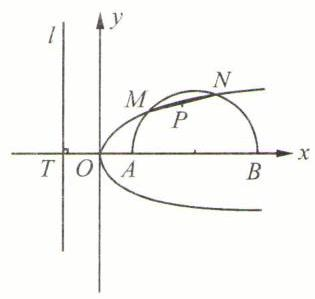
\includegraphics[width=0.2\textwidth]{bodyxb/src/bo_d20cdrf7aajc73bfmvhg_89_1120_519_315_299_0.jpg}
\end{center}


(第 221 题)

$\therefore$ 方程有两个不同的正实根, $\therefore$ 此时点 $M,N$ 存在. 设线段 ${MN}$ 的中点 $P$ 到直线 $l$ 的距离为 ${d}_{3}$ ,则 ${d}_{1} + {d}_{2} = 2{d}_{3}$ . 又点 $P$ 的横坐标为 $\dfrac{{x}_{1} + {x}_{2}}{2} = R - a$ ,故 $\left| {AM}\right|  + \left| {AN}\right|  =$  ${d}_{1} + {d}_{2} = 2\left( {R - a + a}\right)  = {2R}$ . 证毕.

222. 证明:分析:直线与抛物线仅有一个公共点有两种情形:第一,直线与抛物线的对称轴平行

(或重合)；第二,直线与抛物线相切. 在本题中, ${PQ}$ 不能取直径(原因见注释①),此时,被 ${PQ}$ 平分的弦(线段 ${AB}$ )的斜率在不断变化,故至多只有一条被平分的弦与抛物线的对称轴平行 (或重合),而其他则都与抛物线相切. 现设定弦 ${l}_{PQ}$ : $x = a$ ,及其上动点 $M\left( {a,t}\right) \left( {a,t \neq  0,a \neq  0\text{ 的原因请参见注释① };t \neq  0\text{ ，否则 }{AB}\text{ 会与 }{PQ}\text{ 重合). 由垂径定理， }{OM}\bot {AB}\text{ . }}\right)$ 此时 ${l}_{AB} : y - t =  - \dfrac{a}{t}\left( {x - a}\right)$ ,整理得 ${ax} + {ty} - \left( {{a}^{2} + {t}^{2}}\right)  = 0$ . 方法一: (由对称性证存在性) 由于弦 ${PQ}$ 关于 $x$ 轴对称, 故我们猜测抛物线也关于 $x$ 轴对称,即可以写成 ${y}^{2} = m\left( {x - {x}_{0}}\right)$ 的形式. 代入 ${l}_{AB}$ 并消去 $x$ ,得 $\dfrac{a{y}^{2}}{m} + {ty} -$  $\left( {{a}^{2} + {t}^{2} - a{x}_{0}}\right)  = 0$ ,二次项系数 $\dfrac{a}{m} \neq  0$ ,故需使得 $\Delta  = \left( {1 + \dfrac{4a}{m}}\right) {t}^{2} + \dfrac{4{a}^{2}}{m}\left( {a - {x}_{0}}\right)  = 0$ 对任意 $t$ 成立, $\therefore \left\{  \begin{array}{l} 1 + \dfrac{4a}{m} = 0, \\  \dfrac{4{a}^{2}}{m}\left( {a - {x}_{0}}\right)  = 0, \end{array}\right.$ 即 $\left\{  \begin{array}{l} {x}_{0} = a, \\  m =  - {4a}. \end{array}\right.$ 故所有直线都与 ${y}^{2} =  - {4a}\left( {x - a}\right)$ 仅有一个公共点 (相切),存在性得证. 这是顶点在 (a,0),焦点为原点的抛物线. 方法二: (由抛物线的性质同时证明存在性和惟一性) 方法一没有告诉我们所求得的抛物线是不是惟一的. 特别是那些对称轴与坐标轴不平行的抛物线. 为简化计算, 我们使用一个结论: 抛物线焦点在它的任意切线上的射影,必在该抛物线顶点处的切线上. (证明见注释 ②) 设抛物线的焦点为 $F\left( {{x}_{0},{y}_{0}}\right)$ ,在直线 ${AB}$ 上的射影是 ${F}^{\prime }$ . 过焦点 $F$ ,垂直于 ${AB}$ 的直线方程为 ${l}_{F{F}^{\prime }} : y - {y}_{0} = \dfrac{t}{a}\left( {x - {x}_{0}}\right)$ ,与 ${l}_{AB} : y - t =  - \dfrac{a}{t}\left( {x - a}\right)$ 的交点是 ${F}^{\prime }\left( {a + \dfrac{t{x}_{0} - a{y}_{0}}{{t}^{2} + {a}^{2}}}\right.$ , $t$ , $\left. {t - \dfrac{t{x}_{0} - a{y}_{0}}{{t}^{2} + {a}^{2}} \cdot  a}\right)$ ,令 $t = {ka}$ ,可得 ${F}^{\prime }\left( {a + \dfrac{k{x}_{0} - {y}_{0}}{{k}^{2} + 1} \cdot  k,{ka} - \dfrac{k{x}_{0} - {y}_{0}}{{k}^{2} + 1}}\right)$ . 根据分析,并运用以上结论,可知当 $t$ 变化时, 至多除了 1 个 $t$ (或 $k$ ) 对应的 ${F}^{\prime }$ 以外,其他 ${F}^{\prime }$ 均在同一条直线上,设直线为 ${Ax} + {By} + C = 0(A$ 和 $B$ 不能同时为 0 ),代入 ${F}^{\prime }$ 的坐标,整理得 ${aB} \cdot  {k}^{3} + \left\lbrack  {A\left( {a + {x}_{0}}\right)  + C}\right\rbrack   \cdot  {k}^{2} + \left( {-A{y}_{0} + {aB} - {x}_{0}B}\right)  \cdot  k + \left( {{Aa} + B{y}_{0} + C}\right)  = 0$ ,因此 $\left\{  {\begin{array}{l} {aB} = 0, \\  A\left( {a + {x}_{0}}\right)  + C = 0, \\   - A{y}_{0} + {aB} - {x}_{0}B = 0, \\  {Aa} + B{y}_{0} + C = 0, \end{array}\text{ 解得 }\left\{  {\begin{array}{l} {x}_{0} = 0, \\  {y}_{0} = 0, \\  B = 0 \\  {Aa} + C = 0. \end{array}\text{ 因此,如果存在这样的抛物线,那一定以 }\left( {0,0}\right) }\right. }\right.$ 为焦点, $x = a$ 为过顶点的切线,故对称轴必为 $x$ 轴,方程必为 ${y}^{2} =  - {4a}\left( {x - a}\right)$ ,且不难验证 (或由方法一),此时不论点 $M$ 处在什么位置,都有直线 ${AB}$ 与 ${y}^{2} =  - {4a}\left( {x - a}\right)$ 相切. 因此,存在惟一的抛物线 ${y}^{2} =  - {4a}\left( {x - a}\right)$ 满足题意,证毕. 存在性和惟一性均得证. 注: ① 若 $a = 0$ ,即定弦为圆的直径,此时任意过圆心的弦 (不与 $x = 0$ 重合) 都满足条件,所有这些弦几乎 (除了 $x = 0$ 但 $y \neq  0$ ) 充满了整个 ${xOy}$ 平面,因此不存在抛物线满足题意. ②结论的证明: 不妨设抛物线为 ${x}^{2} = {2py}$ ,在抛物线上一点 $S\left( {{x}_{S},{y}_{S}}\right)$ 处,切线斜率是 $\dfrac{{x}_{S}}{\rho }$ (可设直线斜率为 $k$ ,代入抛物线后令 $\Delta  = 0$ 求解),进而得到切线方程 $y - {y}_{S} =$  $\dfrac{{x}_{S}}{p}\left( {x - {x}_{S}}\right)$ ,即 ${x}_{S}x = p\left( {y + {y}_{S}}\right)$ . 抛物线在顶点处的切线是 $y = 0$ . 当切点是(0,0)时,结论成立; 当 ${x}_{S} \neq  0$ 时,切点不为 (0,0),自抛物线焦点向切线 ${x}_{S}x = p\left( {y + {y}_{S}}\right)$ 所引垂线的方程为 $y - \dfrac{p}{2} =  - \dfrac{p}{{x}_{S}} \cdot  x$ ,联立切线、垂线方程可得焦点在切线上的射影是 ${S}^{\prime }\left( {\dfrac{p{y}_{s}}{{x}_{s}},0}\right)$ ,在顶点处的切线 $y = 0$ 上,证毕. ③ 关于方法二的解题思路:抛物线的焦点、顶点、准线中,任意知道两者,就能确定抛物线. 在本题中,我们几乎没有关于焦点、顶点、准线的任何信息,但知道动直线 ${AB}$ 几乎总与抛物线相切. 因此, 以抛物线的切线为媒介, 寻找焦点、顶点、准线之间的关系, 便是自然而然的想法. 因为不难从方法一得到的抛物线看出: ${OM} \bot  {AB}$ 于点 $M$ ,即焦点在切线 ${AB}$ 上的射影,都在直线 ${PQ}$ 上这一特点,所以我们可以猜想这一结论.

